\documentclass[11pt,twoside,openright,spanish]{report}
\usepackage[utf8]{inputenc}
\usepackage[spanish,es-tabla,mexico]{babel}
\usepackage{UNAMThesis}
\usepackage{titlesec, blindtext, color}
\usepackage{amsmath}
\usepackage{amsfonts}
\usepackage{fancyhdr}   
\usepackage{tensor}
\usepackage{multirow} 
\usepackage{tabu}
\usepackage[style]{fncychap}
\usepackage{makeidx}
\usepackage{emptypage}
\usepackage{floatrow}
\usepackage{mathrsfs}
\usepackage[font=footnotesize,labelfont=bf]{caption} % Pie de figura
\usepackage{tabulary}
\usepackage[top=0.8in]{geometry} % Margen superior más adecuado
\usepackage{makeidx}
\usepackage{verbatim}
\usepackage{float} % Permite poner las imágenes en donde queramos
\usepackage{amssymb}
\usepackage{subfig}
\usepackage{layout}
\usepackage{calligra} 
\usepackage[dvipsnames,table,xcdraw]{xcolor}
\usepackage{graphicx} % Nos permite utilizar imágenes.
\usepackage{graphics}
\usepackage{caption}
\usepackage{mwe}
\usepackage{hyperref}
\usepackage{framed}
\usepackage{leftidx}
\usepackage{dsfont}
\usepackage{mathtools}
\usepackage{enumerate}
\usepackage{chngcntr} % Para no resetear notas de pie de página
\usepackage{setspace}
\usepackage{epstopdf}
\usepackage{setspace}
\usepackage{booktabs}
\usepackage{url}
\usepackage{calc}  
\usepackage{calrsfs}
\usepackage{enumitem}
\usepackage[T1]{fontenc}
\usepackage[bitstream-charter]{mathdesign}
\usepackage{etoolbox}
% code listing settings
\usepackage{listings}
\usepackage{wrapfig,lipsum,booktabs}
\usepackage[customcolors,shade]{hf-tikz}
\usepackage[authoryear,round]{natbib}

\DeclareFloatVCode{myrowsep}{\vskip 4ex}

\newcounter{bibcount}
\makeatletter
\patchcmd{\@lbibitem}{\item[}{\item[\hfil\stepcounter{bibcount}{\thebibcount.}}{}{}
\setlength{\bibhang}{2\parindent}
\renewcommand\NAT@bibsetup%
[1]{\setlength{\leftmargin}{\bibhang}\setlength{\itemindent}{-\parindent}%
	\setlength{\itemsep}{\bibsep}\setlength{\parsep}{\z@}}
\makeatother


\bibliographystyle{apalike2mod}

\hfsetbordercolor{blue}

\captionsetup[table]{position=bottom}

\lstset{
	language=Fortran,
	basicstyle=\ttfamily\tiny,
	aboveskip={1.0\baselineskip},
	belowskip={1.0\baselineskip},
	columns=fixed,
	extendedchars=true,
	breaklines=true,
	tabsize=3,
	prebreak=\raisebox{0ex}[0ex][0ex]{\ensuremath{\hookleftarrow}},
	frame=lines,
	showtabs=false,
	showspaces=false,
	showstringspaces=false,
	keywordstyle=\color[rgb]{0.57,0.36,0.51},
	commentstyle=\color[rgb]{0.36,0.54,0.66},
	stringstyle=\color[rgb]{0.59,0.29,0},
	numberstyle=\scriptsize,
	stepnumber=1,
	numbersep=10pt,
	captionpos=t,
	escapeinside={\%*}{*)}
}


\apptocmd{\thebibliography}{\csname cleardoublepage phantomsection\endcsname\addcontentsline{toc} {chapter}{Bibliografía}}{}{}

\makeatletter
\patchcmd{\ttlh@hang}{\parindent\z@}{\parindent\z@\leavevmode}{}{}
\patchcmd{\ttlh@hang}{\noindent}{}{}{}
\makeatother

\numberwithin{equation}{chapter}
\numberwithin{figure}{chapter}
\numberwithin{table}{chapter}
\counterwithout{footnote}{chapter}

\renewcommand{\arraystretch}{1.2}

%Interlineado
\renewcommand{\baselinestretch}{1.5}

\setlength{\headheight}{15pt} 

\logounam{images/Escudo-UNAM}
\logoinstitute{images/Escudo-IBT}
\pagenumbering{roman}
\flushbottom
\newtheorem{theorem}{Theorem}
\newtheorem{acknowledgement}[theorem]{Acknowledgement}
\newtheorem{algorithm}[theorem]{Algorithm}
\newtheorem{axiom}[theorem]{Axiom}
\newtheorem{case}[theorem]{Case}
\newtheorem{claim}[theorem]{Claim}
\newtheorem{conclusion}[theorem]{Conclusion}
\newtheorem{condition}[theorem]{Condition}
\newtheorem{conjecture}[theorem]{Conjecture}
\newtheorem{corollary}[theorem]{Corollary}
\newtheorem{criterion}[theorem]{Criterion}
\newtheorem{definition}[theorem]{Definition}
\newtheorem{example}[theorem]{Example}
\newtheorem{exercise}[theorem]{Exercise}
\newtheorem{lemma}[theorem]{Lemma}
\newtheorem{notat}[theorem]{Notat}
\newtheorem{problem}[theorem]{Problem}
\newtheorem{proposition}[theorem]{Proposition}
\newtheorem{remark}[theorem]{Remark}
\newtheorem{solution}[theorem]{Solution}
\newtheorem{summary}[theorem]{Summary}
\newenvironment{proof}[1][Proof]{\textbf{#1.} }{\ \rule{0.5em}{0.5em}}

\newcommand{\grad}{\hspace{-2mm}$\phantom{a}^{\circ}$}



\renewcommand{\sin}{\operatorname{\sen}}

\lfoot[]{}
\cfoot[]{}
\rfoot[]{}
\renewcommand{\footrulewidth}{0pt}
\renewcommand{\headrulewidth}{0.1pt}

%%%%%%%%%%%%%%%%%%%% Reemplazamos l con elle %%%%%%%%%%%%%%%%%%%%%%
\mathcode`l="8000
\begingroup
\makeatletter
\lccode`\~=`\l
\DeclareMathSymbol{\lsb@l}{\mathalpha}{letters}{`l}
\lowercase{\gdef~{\ifnum\the\mathgroup=\m@ne \ell \else \lsb@l \fi}}%
\endgroup

%%%%%%%%%%%%%%%%%%%%% Norma y valor absoluto %%%%%%%%%%%%%%%%%%%%%%
\DeclarePairedDelimiter\abs{\lvert}{\rvert}%
\DeclarePairedDelimiter\norm{\lVert}{\rVert}%

% Swap the definition of \abs* and \norm*, so that \abs
% and \norm resizes the size of the brackets, and the 
% starred version does not.
\makeatletter
\let\oldabs\abs
\def\abs{\@ifstar{\oldabs}{\oldabs*}}
\let\oldnorm\norm
\def\norm{\@ifstar{\oldnorm}{\oldnorm*}}
%%%%%%%%%%%%%%%%%%%%%%%%%%%%%%%%%%%%%%%%%%%%%%%%%%%%%%%%%%%%%%%%%%%
% Change Colors https://en.wikibooks.org/wiki/LaTeX/Colors
\hypersetup{
	bookmarks=true,         % show bookmarks bar?
	unicode=true,          % non-Latin characters in Acrobat’s bookmarks
	pdftoolbar=true,        % show Acrobat’s toolbar?
	pdfmenubar=true,        % show Acrobat’s menu?
	pdffitwindow=false,     % window fit to page when opened
	pdfstartview={FitH},    % fits the width of the page to the window
	pdftitle={Tesis Uzmar},    % title
	pdfauthor={Uzmar Gómez},     % author
	pdfsubject={Subject},   % subject of the document
	pdfcreator={Uzmar Gómez},   % creator of the document
	pdfproducer={Uzmar Gómez}, % producer of the document
	pdfkeywords={}, % list of keywords
	pdfnewwindow=true,      % links in new PDF window
	colorlinks=true,       % false: boxed links; true: colored links
	linkcolor=BlueViolet,          % color of internal links (change box color with linkbordercolor)
	citecolor=BrickRed,        % color of links to bibliography
	filecolor=NavyBlue,      % color of file links
	urlcolor=NavyBlue           % color of external links
}
 
 
\newenvironment{changemargin}[3]{
	\begin{list}{}{
			\setlength{\topsep}{#3}
			\setlength{\leftmargin}{#1}
			\setlength{\rightmargin}{#2}
			\setlength{\listparindent}{\parindent}
			\setlength{\itemindent}{\parindent}
			\setlength{\parsep}{\parskip}
		}
		\item[]}{\end{list}}

\begin{document}
	
\renewcommand{\baselinestretch}{1}

\graphicspath{{./images/}}

\title{Estudio numérico de la ecuación de Vlasov en la métrica de Schwarzschild: La materia obscura en la vecindad de un agujero negro.}
\author{Uzmar de Jesús Gómez Yáñez}
\institute{Facultad de Ciencias}
\degree{Físico}
\supervisor{Dr. Miguel Alcubierre Moya}
\city{Ciudad Universitaria, CD. MX.}
\degreemonth{Septiembre}
\degreeyear{2018}
\maketitle

\newpage
$\ $
\thispagestyle{empty} % para que no se numere esta pagina

\begin{changemargin}{1cm}{0cm}{1cm}
	
	\vspace{30cm} 
	\begin{center}
		\textit{\textbf{\Large JURADO ASIGNADO}}
	\end{center}
	\vspace{1cm}
	\noindent
	\begin{description}
		\item[]\textbf{Datos del alumno:}\\
		Gómez Yáñez, Uzmar de Jesús\\
		\textit{Número de cuenta:} 308287141\\
		\textit{Institución de adscripción:} Facultad de Ciencias, UNAM\\
		\textit{Carrera:} Física\\
		\textit{Correo:} uzmar.gomez@ciencias.unam.mx\\
		\textit{Teléfono:} 5539347885
		\vspace{1cm}
		
		\item[]\textbf{Presidente:}\\
		Dr. Núñez Zúñiga, Darío\\
		\textit{Correo:} nunez@nucleares.unam.mx\\
		\textit{Institución de adscripción:} Instituto de Ciencias Nucleares, UNAM
		\item[]\textbf{Vocal:}\\
		Dr. Matos Chassin, Tonatiuh\\
		\textit{Correo:} tmatos@fis.cinvestav.mx \\
		\textit{Institución de adscripción:} Departamento de Física, CINVESTAV
		\item[]\textbf{Secretario:}\\
		Dr. Alcubierre Moya, Miguel\\
		\textit{Correo:} malcubi@nucleares.unam.mx\\
		\textit{Institución de adscripción:} Instituto de Ciencias Nucleares, UNAM
		\item[]\textbf{1\textsuperscript{er} Suplente:}\\
		Dr. Tejeda Rodríguez, Emilio\\
		\textit{Correo:} etejeda@astro.unam.mx\\
		\textit{Institución de adscripción:} Instituto de Astronomía, UNAM
		\item[]\textbf{2\textsuperscript{do} Suplente:}\\
		Dr. Degollado Daza, Juan Carlos\\
		\textit{Correo:} jcdegollado@ciencias.unam.mx\\
		\textit{Institución de adscripción:} Instituto de Ciencias Físicas, UNAM
	\end{description}
\thispagestyle{empty}
\end{changemargin}


%\ChNameVar{\bfseries\Large\sf} \ChNumVar{\Huge} \ChTitleVar{\bfseries\Large\rm}
%\ChRuleWidth{1pt} \ChNameUpperCase \ChTitleUpperCase
\ChNumVar{\fontsize{50}{50}\usefont{T1}{ptm}{m}{sl}\selectfont}
\ChTitleVar{\raggedright\Large\sffamily\bfseries}

\evensidemargin 0in 
\oddsidemargin 0.6in

\newpage{\ } 
\thispagestyle{empty}

\begin{dedication}
{\Large{\calligra{Recuerda mirar hacia arriba a las estrellas y no abajo hacia tus pies. Trata de darle sentido a lo que ves y pregúntate qué hace que el universo exista. Sé curioso, y por más dura que la vida pueda parecer, siempre hay algo que puedes hacer y tener éxito en ello. Lo importante es que nunca te des por vencido.}}}\\
\begin{comment}
{\footnotesize{\dots black holes ain't as black as they are painted. They are not the eternal prisons they were once though\dots things can get out of a black hole both on the outside and possibly to another universe. So if you feel you are in a black hole, don’t give up, there’s a way out.}}\\
\end{comment}
\vspace{0.5cm}
{\scriptsize{\bfseries{Stephen Hawking}}}
\end{dedication}

\newpage
$\ $
\thispagestyle{empty} % para que no se numere esta pagina

\begin{acknowledgements}
\pagenumbering{Roman}
\noindent
A mi asesor el Dr. Miguel Alcubierre Moya, por todo el apoyo académico que me dio; por sus consejos, sus enseñanzas, y por la paciencia y dedicación que tuvo para que lograra sacar adelante este trabajo. Le agradezco por impartir las mejores asignaturas que he tenido en la carrera, las cuales me permitieron descubrir lo interesante y bella que es la teoría de la Relatividad, y lo divertido que es programar. Gracias por darme la oportunidad de trabajar y aprender de usted, será siempre mi ejemplo a seguir.
\\

\noindent
A mis sinodales, los doctores Darío Nuñéz Zúñiga, Tonatiuh Matos Chassin, Emilio Tejeda Rodríguez y Juan Carlos Degollado Daza, por sus revisiones y comentarios, los cuales enriquecieron y mejoraron mucho este trabajo. Quiero agradecer de manera muy especial a los estudiantes tanto del Dr. Alcubierre como del Dr. Núñez, los ahora físicos Erik Rodrigo Jiménez Vázquez y Paola Domínguez Fernández, cuyo trabajo previo fue de enorme ayuda para concluir mi tesis.
\\

\noindent
A mi mamá Olivia de Jesús Yáñez Narváez, quién me alentó a seguir adelante y a superarme, apoyándome en todo lo que necesité. En tí descubrí a una mujer admirable, amorosa, fuerte y dedicada. Prometo ser cada día mejor, para que te sientas tan orgullosa de mí como yo lo he estado siempre de tí. Eres mi amor más grande.
\\

\noindent
A mi abuelita Bertha Narváez Ramos, mi primer maestra, gracias por esos días de enseñarme las tablas de multiplicar y a resolver ecuaciones de primer grado (sin olvidar las clases de amarrar agujetas), quizá por ellos fue que terminé en un área tan afín a las matemáticas como es la física. Gracias por nunca perder tu confianza en mí, por los valores que me inculcaste, a tí te debo ser la persona que soy el día de hoy. Te amo infinitamente.
\\

\noindent
A mi hermano Christopher Gómez Yáñez, por siempre mostrarme que estás ahí incondicionalmente, tanto en mis mejores y más felices momentos, como en aquellos de más angustia y pesar. Estaré eternamente agradecido de tener un hermano como tú, recuerda que me haces sentir orgulloso, y deseo que, como hasta ahora, tengas éxito en todo lo que te propongas.
\\

\noindent
A mi novia Luisa Alejandra Granados Hernández quién, desde que la conocí, no solo me ayudó a ser una mejor persona y me impulsó a cumplir mis metas, sino que me apoyó a lo largo de mi carrera hasta que (al fin!) llegó a su conclusión. Espero seguir viviendo más momentos contigo, me siento feliz de ver lo que has logrado, de tí aprendí que no existe ningún obstáculo que no pueda ser superado con esfuerzo y constancia.
\\

\noindent
A mi mejor amigo Raúl Puente Mancilla, quién me mostró cómo sobrevivir a la dura vida que tiene un biólogo que hace un cambio de carrera a física, que me enseñó a dar lo mejor de mí y a no poner límites a mi esfuerzo, a pesar del cansancio y de los problemas que puedan surgir. Gracias por esas noches enteras que pasamos resolviendo tareas o redactando a última hora nuestras bitácoras, en tí descubrí el verdadero significado de la palabra ``amigo''.   
\\

\noindent
A mis amigos de la facultad: Sally Paredes, Nancy Mondragón, Andrea Mediana, Alejandro Villarreal, Guadalupe Reza y Arturo Nájera. Gracias por permitirme entrar en sus vidas y compartir sus experiencias, y por la ayuda que me brindaron siempre que los necesité.
\\

\noindent
A la UNAM, institución que quiero y respeto por haber aceptado que entrara en sus aulas hace ya algunos años, y por haberme permitido estudiar algo que tanto amo, la física. Procuraré siempre poner en alto su nombre.
\\

\noindent
A los profesores que he tenido la dicha de conocer, les debo mis éxitos futuros. Muchas gracias!
\\


\end{acknowledgements}


\tableofcontents


\addtolength{\headheight}{\baselineskip}
\fancyhead[LE]{\scshape\thepage\hspace{1cm}\footnotesize\nouppercase{Universidad Nacional Autónoma de México}}
\fancyhead[RO]{\scshape\footnotesize\nouppercase{Facultad de Ciencias}\hspace{1cm}\normalsize\thepage}
\pagestyle{fancy}
\cleardoublepage

\begin{notation}
	\addcontentsline{toc}{chapter}{\numberline{}Notación}%	
	\pagenumbering{arabic}
	\noindent
	En este trabajo se utiliza la convención de Misner, Thorne y Wheeler\footnote{Ver \citet{MTW}, p. 9.}, es decir, los índices espacio-temporales irán de 0 a 3, siendo 0 la coordenada temporal, y se denotarán con índices griegos. Los índices latinos se utilizarán para denotar únicamente el espacio tridimensional. Además, se utilizará la convención de suma de Einstein y las unidades geométricas, las cuales toman a la velocidad de la luz $c$ y a la constante gravitacional $G$ iguales a uno. Así, todas las cantidades físicas tienen dimensiones de distancia. De esta manera, por ejemplo, las unidades de distancia, tiempo y masa son metros (la \textit{unidad} se denotará como ``$\text{m}$'', para diferenciarla de la \textit{variable} ``$m$'').
	
	La derivada parcial respecto a la coordenada $x^\mu$ de una cierta cantidad geométrica $V$, se denotará como $\partial_\mu V$ o como $\frac{\partial V}{\partial x^\mu}$ indistintamente, y la derivada covariante se denotará como $\nabla_\mu V$ en cuatro dimensiones y $D_i V$ en tres dimensiones. Los tensores asociados a la métrica tridimensional $\gamma_{ij}$ se denotarán con un superíndice ``(3)'' en su lado izquierdo, por ejemplo, $^{(3)}\tensor{T}{^\alpha_\beta}$, y los asociados a la métrica $g_{\alpha\beta}$ no tendrán ningún símbolo extra. Asimismo, se utiliza $g$ para denotar el determinante de la métrica espacio-temporal y $\gamma$ para el determinante de la métrica puramente espacial.
\end{notation}

\begin{preface}
\addcontentsline{toc}{chapter}{\numberline{}Prefacio}%	

En este trabajo se buscó obtener un método numérico utilizando diferencias finitas, que permita evolucionar la ecuación de Vlasov relativista bajo la influencia de una métrica de fondo, tomando un conjunto de partículas definidas por una función de distribución como condición inicial. Esta métrica se tomó como la de Schwarzschild, la cual describe un objeto esféricamente simétrico y estático, en particular, un agujero negro. Se utilizaron dos coordenadas que describen esta misma métrica, las de Schwarzschild y las de Kerr-Schild, principalmente debido a que estas últimas penetran el horizonte de eventos. 

Se tomó una aproximación estadística de este estudio, y por lo mismo, se procuró que los métodos en diferencias finitas describieran la evolución de la función de distribución de la manera más precisa posible, siendo que todas las cantidades útiles se pueden obtener de cuadraturas que incluyen esta función de distribución. Por lo mismo, se bucaron métodos que no generaran oscilaciones espurias ni dispersión; para lograr lo anterior, se utilizaron métodos conocidos como conservadores de flujo.

Los resultados son los esperados dado el problema planteado, es decir, si la métrica no evoluciona entonces dado un momento angular mayor a $\sqrt{12}\ M$, deben existir partículas que se queden en una órbita circular estable, y para un momento angular menor a $\sqrt{12}\ M$, todas las partículas deben de caer al agujero negro. Se concluye que el método numérico converge, es estable y consistente para este problema, sin embargo, esto es solo un primer intento que, se espera, permita una generalización al caso en el que la métrica cambie debido a la evolución de las fuentes de masa descritas por la función de distribución, representada en las ecuaciones de Einstein por un tensor de energía momento.
\end{preface}

%--------------------------------------------------------------------------------------------------------------- %

\fancypagestyle{plain}{
	\fancyhead[L]{}
	\fancyhead[C]{}
	\fancyhead[R]{}
	
	\fancyfoot[L]{}
	\fancyfoot[C]{\thepage}
	\fancyfoot[R]{}
	\renewcommand{\headrulewidth}{0pt}
	\renewcommand{\footrulewidth}{0pt}
}

\fancyhead[LE]{\scshape\thepage\hspace{1cm}\footnotesize\nouppercase{\leftmark}}
\fancyhead[RO]{\scshape\footnotesize\nouppercase{Sección \rightmark\hspace{1cm}}\normalsize\thepage}
\fancyhead[LO]{}
\fancyhead[RE]{}
\pagestyle{fancy}
\cleardoublepage

\chapter{Introducción}\label{cap:Introducción}
\noindent
En este capítulo se introduce brevemente la teoría e historia de los agujeros negros y la materia obscura, haciendo énfasis en el porqué puede explicarse la dinámica de esta última mediante la ecuación de Boltzmann no colisional. Asimismo, se introducen las bases de la relatividad numérica desde el punto de vista del formalismo 3+1, y se trata el caso particular de simetría esférica en dicho formalismo. Además, se habla sobre el Teorema del Virial debido a su utilidad en el estudio de la estabilidad de los métodos numéricos asociados a la ecuación de Vlasov.

\section{Agujeros Negros y Materia Obscura}
\noindent
Un agujero negro (en inglés, \textit{Black Hole}\footnote{Este término fue adoptado por John Wheeler después de dar una conferencia en 1967, cuando alguien en la audiencia lo dijo de manera casual como una forma de resumir \textit{``Gravitationally Completely Collapsed Star''} o ``Estrella completamente colapsada''. Así, fue Wheeler quien popularizó el término, pero no se sabe con certeza quién lo inventó. Ver \citet{quinionbh}.}) fue la primera solución teórica exacta a las ecuaciones de Einstein, encontrada por el astrónomo alemán Karl Schwarzschild, que describía de manera exacta el campo gravitacional fuera de una estrella esférica\footnote{Ver \citet{schutzgftgu}.}. Físicamente, un agujero negro posee una masa que puede llegar a ser más grande de $10^{10}\ M_{\odot}$\footnote{El símbolo $M_{\odot}$ representa una ``masa solar'', que es una unidad de medición igual a la masa del Sol. Su valor es de $1.989\times10^{30}\ \text{kg}$.}, y es aquello que queda después de que un objeto ha pasado por un colapso gravitacional. Debido a su gran fuerza gravitacional\footnote{Derivada de su compacticidad, es decir, el cociente de su masa entre su radio.}, el espacio-tiempo se curva fuertemente, de manera que nada puede escapar de su influencia, ni siquiera la luz, una vez que se cruza una cierta superficie crítica conocida como ``horizonte de eventos''\footnote{Ver \citet{ruffiniitbh}.}. En este trabajo se analiza el intervalo espacio-temporal descrito por Schwarzschild, que posee una singularidad en el horizonte de eventos, además, debido a que dicha singularidad es generada por las coordenadas escogidas y no una que describa algo físico, se hace un cambio de coordenadas que nos permitirá estudiar qué sucede dentro del agujero negro (sin llegar al origen); a estas coordenadas se les conoce como de \emph{Kerr-Schild}.

La materia obscura es, en términos generales, aquella que no emite radiación. Existen dos tipos, la conocida como \textit{bariónica}, que es aquella formada por protones, electrones y neutrones, y la \textit{no bariónica} (o simplemente materia obscura, nombre que se le da comúnmente y como se refiere de aquí en adelante en este escrito), un tipo de materia que hasta la fecha no ha logrado detectarse en el laboratorio. Su estudio comenzó en 1937, cuando Fritz Zwicky concluyó que la alta velocidad de las galaxias que él observó en el cúmulo de galaxias ``Coma'', precisaba de la existencia de materia obscura, ya que la masa total del cúmulo calculada por las velocidades obtenidas excedía la suma de las masas bariónicas de los componentes individuales\footnote{Ver \citet{trimbleeanodmitu}.}. En 1970, Vera Rubin midió las curvas de rotación de galaxias individuales y descubrió que, contrario a lo que se pensaba (esto es, que dado que la fuerza de gravedad y, por tanto, la masa de una Galaxia, determina la velocidad de las estrellas orbitándola, estas últimas deberían rotar más lentamente a medida que se alejan del centro de la misma), la velocidad de las estrellas que orbitaban el centro de una galaxia era constante sin importar qué tan lejos estuvieran del centro, implicando así que la masa de las galaxias incrementa con el radio, por lo que debe existir una cantidad muy grande de materia que no se puede observar en las mismas \footnote{Ver \citet{Hunter2017}.}. 

Estos datos, además de los estudios realizados en la actualidad, revelan que no solamente existe la materia obscura, sino que además la mayor parte de la materia en el Universo no está compuesta por bariones o alguna otra de las partículas conocidas actualmente sino que, de hecho, sucede que la cantidad de materia obscura es al menos cinco veces más abundante que la cantidad de materia visible, y constituye alrededor de una cuarta parte del Universo. A pesar de lo anterior, aún no se sabe siquiera qué partícula podría ser la que constituya este tipo de materia, aunque existen varios candidatos, como son los WIMPs (\textit{Weakly interacting massive particles}, que se traduce como ``partículas masivas que interactúan débilmente''), superWIMPs, gravitones ligeros, axiones, entre otros\footnote{Ver \citet{fengdmcfppamod}.}.

Sin embargo, vale la pena mencionar que la existencia de la materia obscura esta únicamente basada en sus efectos gravitacionales, y aunado a que no interactúa con las ondas electromagnéticas, hace que su estudio sea muy complicado, al grado que hay científicos que dudan de esta teoría\footnote{Existen teorías alternativas a la materia obscura, tales como la ``Dinámica Newtoniana Modificada'' (MOND por sus siglas en inglés), o teorías de ``Gravedad modificada f(R)''. Ver \citet{Gentile2018} y \citet{Lobo2009}.}. Dichos efectos gravitacionales son parecidos a los provocados por la materia bariónica; además, se ha encontrado que la materia obscura puede intercambiar energía únicamente mediante interacciones gravitacionales elásticas, por lo que es posible el análisis de su dinámica mediante un tratamiento estadístico, y en particular con la ecuación de Boltzmann no colisional\footnote{Ver \citet{ostrikernlodm}.}.


\section{Formalismo 3+1}\label{formalismo31}
\noindent
El formalismo 3+1 de la relatividad numérica consiste en hacer una separación del espacio-tiempo en tres dimensiones espaciales y una temporal, de manera que sea posible evolucionar un cierto campo gravitacional partiendo de un problema de valores iniciales (conocido en el área de ecuaciones diferenciales como problema de Cauchy), en particular, las cantidades a especificar a un tiempo inicial son la métrica $g_{\alpha\beta}$ y su derivada temporal $\partial_tg_{\alpha\beta}$ en una hipersuperficie espacial 3-dimensional. Así, dadas las condiciones iniciales sobre estas variables (mismas que deben cumplir con las ecuaciones de constricción que se mencionarán posteriormente) y ecuaciones de evolución sobre las fuentes materiales, es posible obtener el comportamiento del sistema en estudio a distintos tiempos\footnote{Ver \citet{alcubierre}, capítulo 2.}. 

Se considerará un espacio-tiempo con una métrica $g_{\mu\nu}$ al que se le realiza una foliación tal que las hojas de dicha foliación son hipersuperficies tridimensionales espacialoides. Estas superficies dependen de un parámetro $t$ y se denotan como $\Sigma_t$. Dadas dos de estas hipersuperficies $\Sigma_t$ y $\Sigma_{t+\text{d}t}$, se presupone que la distancia $\text{d}t$ que las separa es infinitesimal.

Para describir la geometría del espacio-tiempo es necesario definir dos objetos matemáticos: la función de ``lapso'' $\alpha$ y el ``vector de corrimiento'' $\beta^i$. El primero de estos determina el lapso de tiempo propio $\tau$ entre dos hipersuperficies adyacentes que mide un observador que se mueve en dirección normal a las foliaciones, es decir
\begin{equation}
	\text{d}\tau=\alpha\left(t,x^i\right)\ \text{d}t
\end{equation}
Finalmente, $\beta^i$ mide cuánto se mueven las coordenadas espaciales respecto del vector normal sobre la hipersuperficie
\begin{eqnarray}
	x_{t+\text{d}t}^i=x_t^i-\beta^i\left(t,x^j\right)\ \text{d}t
\end{eqnarray}
De esta manera, se concluye que la función de lapso y el vector de corrimiento determinan la evolución de las coordenadas al pasar de una cierta hipersuperficie $\Sigma_t$ a una hipersuperficie vecina $\Sigma_{t+\text{d}t}$. 

Si $n^{\mu}$ es el vector unitario normal a $\Sigma_t$, definido como $n^\mu=\left(\frac{1}{\alpha},-\frac{\beta^i}{\alpha}\right)$ y $n_\mu=\left(-\alpha,0\right)$, entonces la métrica espacio temporal $g_{\mu\nu}$ induce una métrica espacial $\gamma_{\mu\nu}$ sobre $\Sigma_t$ que viene dada por
\begin{equation}
\gamma_{\mu\nu}=g_{\mu\nu}+n_\mu n_\nu, \hspace{1cm}\gamma^{\mu\nu}=g^{\mu\nu}+n^\mu n^\nu, \hspace{1cm}\tensor{\gamma}{^\mu_\nu}=\tensor{\delta}{^\mu_\nu}+n^\mu n_\nu
\end{equation}
siendo esta métrica un tensor que proyecta todos los objetos geométricos sobre $\Sigma_t$, especificada por su vector normal $n^\mu$, y permite medir distancias en dicha hipersuperficie, además de ser puramente espacial.

Usando lo anterior, se puede escribir el elemento de línea invariante de manera general en el formalismo 3+1 de la siguiente forma
\begin{equation}
\text{d}S^2=\left(-\alpha^2+\beta_i \beta^i\right)\ \text{d}t^2 + 2\beta_i\ \text{d}x^i\ \text{d}t+ \gamma_{ij}\ \text{d}x^i\ \text{d}x^j
\end{equation}
donde, debido a que por definición $\gamma_{ij}=g_{ij}$, la subida y bajada de índices espaciales puede realizarse con la métrica espacial $\gamma_{ij}$ y su inversa $\gamma^{ij}$. 

Dicho elemento de línea mide la distancia que existe entre dos puntos en el espacio-tiempo, tomando en cuenta la contribución que viene del tiempo propio que existe entre dos hipersuperficies espacialoides adyacentes, así como también la distancia propia medida dentro de una de estas hipersuperficies. En la figura \ref{foliacion31} se muestra una imagen que describe mejor lo tratado hasta ahora\footnote{Ver \citet{Shapiro2010}, capítulo 2.}.
\begin{figure}[H]
	\centering
	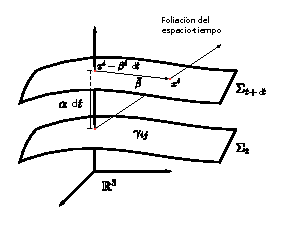
\includegraphics[height=6.7cm]{foliacion31}
	\caption{Foliación del espacio-tiempo en hojas espacialoides, se muestra gráficamente el significado tanto de la función de lapso como del vector de corrimiento.}
	\label{foliacion31}
\end{figure}

Se distingue entre dos tipos de curvatura al momento de trabajar con las hipersuperficies espaciales $\Sigma_t$, la curvatura intrínseca y la extrínseca. La primera proviene de la geometría interna de la hipersuperficie y está determinada por el tensor de Riemann tridimensional $^{(3)}\tensor{R}{^\alpha_\beta_\gamma_\delta}$, asociado a la métrica espacial $\gamma_{ij}$ de manera análoga al tensor de Ricci en el espacio-tiempo. La curvatura extrínseca viene asociada a la forma de las hipersuperficies que están inmersas en el espacio tiempo. Esta curvatura se define en términos del comportamiento del vector normal $n^\alpha$ al ser transportado paralelamente de un lugar a otro de la superficie. El cambio de este vector normal bajo transporte paralelo está dado por el tensor de curvatura extrínseca $K_{\alpha\beta}$.

Este tensor se puede escribir en términos de la métrica espacial como
\begin{equation}
K_{\mu\nu}=-\frac{1}{2}\mathcal{L}_{\vec{n}}\gamma_{\mu\nu}
\label{extcurvtensorlie}
\end{equation}
siendo $\mathcal{L}_{\vec{n}}$ la derivada de Lie a lo largo del vector normal. A partir de la ecuación \eqref{extcurvtensorlie} se obtiene directamente la siguiente expresión usando la definición del vector $t^\gamma=\alpha n^\gamma+\beta^\gamma$
\begin{equation}
\partial_t \gamma_{ij}=-2\alpha K_{ij}+D_j\beta_i+D_i\beta_j
\label{cambioengamma}
\end{equation}
donde $D_i$ es la derivada covariante tridimensional. Dados los elementos anteriores, es posible dar expresiones para la métrica del espacio tiempo y sus símbolos de Christoffel asociados en el lenguaje 3+1\footnote{Ver \citet{alcubierre}, p. 409.}. La 4-métrica y su inversa asociada tienen la forma
\begin{subequations}
	\begin{align}
	g_{00}&=-\left(\alpha^2-\gamma_{ij}\beta^i\beta^j\right) & g^{00}&=-\frac{1}{\alpha^2}\\
	g_{0i}&=\gamma_{ij}\beta^j=\beta_i                       & g^{0i}&=\frac{\beta^i}{\alpha^2}\\
	g_{ij}&=\gamma_{ij}                                      & g^{ij}&=\gamma^{ij}-\frac{\beta^i\beta^j}{\alpha^2}
	\end{align}\label{g}
\end{subequations}
Los símbolos de Christoffel son, en términos de las mismas cantidades del formalismo 3+1
\begin{subequations}
	\begin{align}
	\tensor{\Gamma}{^0_0_0}&=\frac{1}{\alpha}\left(\partial_t\alpha+\beta^m\partial_m\alpha-\beta^m\beta^n K_{mn}\right)\label{geodgen}\\
	\tensor{\Gamma}{^0_0_i}&=\frac{1}{\alpha}\left(\partial_i\alpha-\beta^m K_{im}\right)\\
	\tensor{\Gamma}{^0_i_j}&=-\frac{K_{ij}}{\alpha}\\
	\tensor{\Gamma}{^k_0_0}&=\alpha\partial^k \alpha-2\alpha\beta^m K_m^k -\frac{\beta^k}{\alpha}\left(\partial_t\alpha+\beta^m\partial_m\alpha-\beta^m\beta^nK_{mn}\right)+\partial_t\beta^k+\beta^mD_m\beta^k\\
	\tensor{\Gamma}{^k_m_0}&=-\frac{\beta^k}{\alpha}\left(\partial_m\alpha-\beta^nK_{mn}\right)-\alpha K_m^k+D_m\beta^k\\
	\tensor{\Gamma}{^k_i_j}&=\ ^{(3)}{\tensor{\Gamma}{^k_i_j}}+\frac{\beta^kK_{ij}}{\alpha}
	\end{align}\label{christoffel3+1}
\end{subequations}
siendo $D_i$ la derivada covariante tridimensional y $^{(3)}\tensor{\Gamma}{^k_i_j}$ los símbolos de Christoffel, ambos asociados a la métrica espacial $\gamma_{ij}$.

\subsubsection{Ecuaciones de Einstein y constricciones en simetría esférica}
\noindent
Las ecuaciones de campo de Einstein se pueden escribir en el lenguaje 3+1 utilizando tres ecuaciones, conocidas como ecuaciones de Gauss, Godazzi y Ricci, a continuación resumidas:

\begin{itemize}
	\item \textit{Ecuación de Gauss}
	\begin{equation}
	R_{\alpha\beta\mu\nu}+K_{\alpha\mu}K_{\beta\nu}-K_{\alpha\nu}K_{\mu\beta}=\tensor{\gamma}{^\kappa_\alpha}\tensor{\gamma}{^\lambda_\beta}\tensor{\gamma}{^\rho_\mu}\tensor{\gamma}{^\sigma_\nu}\ R_{\kappa\lambda\rho\sigma}
	\label{eqgauss}
	\end{equation}
	\item \textit{Ecuación de Codazzi}
	\begin{equation}
	D_\beta K_{\alpha\mu}-D_\alpha K_{\beta\mu}=\tensor{\gamma}{^\kappa_\alpha}\tensor{\gamma}{^\lambda_\beta}\tensor{\gamma}{^\rho_\mu}n^\sigma\ R_{\kappa\lambda\rho\sigma}
	\label{eqcodazzi}
	\end{equation}
	\item \textit{Ecuación de Ricci}
	\begin{equation}
	\mathcal{L}_{\vec{n}}K_{\alpha\beta}=n^\nu n^\mu \tensor{\gamma}{^\lambda_\alpha}\tensor{\gamma}{^\rho_\beta}\ R_{\nu\rho\mu\lambda}-\frac{1}{\alpha}D_{\alpha}D_\beta\alpha-\tensor{K}{^\mu_\beta}K_{\alpha\mu}
	\label{eqricci}
	\end{equation}
\end{itemize}

Básicamente, tomando \eqref{eqgauss}, \eqref{eqcodazzi} y \eqref{eqricci}, además de las ecuaciones de Einstein escritas a continuación
\begin{equation}
G_{\alpha\beta}\equiv R_{\alpha\beta}-\frac{1}{2}Rg_{\alpha\beta}=8\pi T_{\alpha\beta}
\end{equation}
donde $T^{\alpha\beta}$ es el tensor de energía-esfuerzos, $R_{\mu\nu}\coloneqq\tensor{R}{^\lambda_\mu_\lambda_\nu}$ es el tensor de curvatura y $R\coloneqq \tensor{R}{^\mu_\mu}$ es el escalar de curvatura, se pueden obtener las ecuaciones conocidas como constricciones Hamiltoniana y de momento\footnote{Una derivación detallada se puede encontrar en \citet{Shapiro2010}, secciones 2.5 y 2.6.}.

La \textit{constricción Hamiltoniana} se escribe
\begin{equation}
R-K_{ij}K^{ij}+K^2=16\pi\rho
\label{constriccionhamiltoniana}
\end{equation}
donde $K=\gamma^{ij}K_{ij}$ es la traza del tensor de curvatura extrínseca y $\rho$ la densidad de energía de la materia según los observadores que se mueven a lo largo de la dirección normal a las hipersuperficies (conocidos como observadores de Euler), tal que $\rho=n^\mu n^\nu T_{\mu\nu}$.

La \textit{constricción de momentos} se escribe
\begin{equation}
D_j[K^{ij}-\gamma^{ij}K]=8\pi S^{i}
\label{constriccionmomentos}
\end{equation}
siendo $D_j$ la derivada covariante respecto a la métrica espacial, y $S_\mu$ la ``densidad de momento'' medida por los observadores de Euler, definida como
\begin{equation}
S_\nu=-\tensor{\gamma}{^\mu_\nu}n^\sigma T_{\mu\sigma}
\end{equation}

Las ecuaciones \eqref{constriccionhamiltoniana} y \eqref{constriccionmomentos} imponen restricciones sobre las condiciones iniciales. Para resolver las ecuaciones de campo de Einstein, estas constricciones deben cumplirse desde el inicio de la evolución.

Proyectando las ecuaciones de Einstein con la hipersuperficie se obtiene
\begin{align}
\nonumber
\partial_t K_{ij}=&\beta^{k}\partial_k K_{ij}+K_{ik}\partial_j \beta^k+K_{jk}\partial_i\beta^k-D_iD_j\alpha\\
&+\alpha\left[R_{ij}+KK_{ij}-2K_{ik}K^k_j\right]+4\pi\alpha\left[\gamma_{ij}\left(S-\rho\right)- 2S_{ij}\right]\label{cambioenk}
\end{align}
siendo $S_{ij}=\gamma_{i\mu}\gamma_{j\nu} T^{\mu\nu}$ el tensor de esfuerzos de la materia en la hipersuperficie $\Sigma_t$ de la foliación, y $S$ su traza. A las ecuaciones \eqref{cambioengamma} y \eqref{cambioenk}, se les conoce como ecuaciones de evolución de Arnowitt-Deser-Misner (ADM)\footnote{Ver \citet{alcubierre}, sección 2.5.}. 

Es posible expresar las constricciones antes mencionadas para el caso general de una simetría esférica (ver apéndice \ref{desarrolloconstadm}), que deben resolverse para ser consistentes con las Ecuaciones de Einstein. Se considera la métrica en el formalismo 3+1 en simetría esférica
\begin{equation}
\text{d}S^2=\left(-\alpha^2+\beta_r\beta^r\right)\ \text{d}t^2+2\beta_r\ \text{d}r\ \text{d}t+\psi^4\left[A\ \text{d}r^2+Br^2\left(\text{d}\theta^2+\sin^2\theta\ \text{d}\phi^2\right)\right]
\label{metricaesfericaespacial}
\end{equation}
donde se introdujo un factor $\psi$, que permite hacer una transformación conforme\footnote{Una función es llamada mapeo conforme si preserva ángulos de localmente. Ver \citet{marsdencompleja}.} de la métrica espacial $\gamma_{ij}=\psi^4\overline{\gamma}_{ij}$, siendo $\overline{\gamma}_{ij}$ la llamada métrica conforme\footnote{Esto no es más que un truco matemático que permite reescribir una incógnita como el producto de dos incógnitas, haciendo que el resolver las ecuaciones se vuelva más fácil. Ver \citet{Shapiro2010}, p. 56. Por lo anterior, a $\psi$ se le conoce como ``factor conforme''}. Las constricciones para la parte puramente espacial de la métrica escrita en la ecuación \eqref{metricaesfericaespacial} se reducen a
\begin{align}
\nonumber
H=&-\partial_r D_B-\frac{3D_B^2}{4}+\frac{D_A D_B}{2}+\frac{1}{r}\left(D_A-3D_B\right)\\
&+\frac{1}{r^2B}\left(A-B\right)+AK_B\left(2K_A+K_B\right)-8\pi A\rho=0
\label{consthamiltonianaesferica}\\
M=&-\partial_r K_B+\left(K_A-K_B\right)\left[\frac{1}{r}+\frac{D_B}{2}\right]-4\pi S_r=0
\label{constmomentoesferica}
\end{align}
siendo $K_A\coloneqq K_r^r$, $K_B\coloneqq K_{\theta}^{\theta}=K_{\phi}^\phi$, $D_A\coloneqq\partial_r\ln A$ y  $D_B\coloneqq\partial_r \ln B$, y donde $S_r$ es la densidad de momento en la dirección radial.

A continuación se escriben las ecuaciones ADM a primer orden para simetría esférica obtenidas de \eqref{cambioengamma} y \eqref{cambioenk}, que para un vector de corrimiento nulo y $\psi=1$ son
\begin{subequations}
	{\small
	\begin{align}
	\partial_tA=&-2\alpha AK_A\\
	\partial_tB=&-2\alpha BK_B\\
	\partial_tD_A=&-2\alpha\left[K_AD_\alpha+\partial_rK_A\right]\\
	\partial_tD_B=&-2\alpha\left[K_BD_\alpha+\partial_rK_B\right]\\
	\nonumber
	\partial_tK_A=&-\frac{\alpha}{A}\left[\partial_r\left(D_\alpha+D_B\right)+D_\alpha^2-\frac{D_\alpha D_A}{2}+\frac{D_B^2}{2}-\frac{D_AD_B}{2}\right.\\
	&\left.-AK_A\left(K_A+2K_B\right)-\frac{1}{r}\left(D_A-2D_B\right)\right]+4\pi\alpha M_A\\
	\nonumber
	\partial_tK_B=&-\frac{\alpha}{2A}\left[\partial_rD_B+D_\alpha D_B+D_B^2-\frac{D_AD_B}{2}-\frac{1}{r}\left(D_A-2D_\alpha-4D_B\right)\right.\\
	&\left.-\frac{2\left(A-B\right)}{r^2B}\right]+\alpha K_B\left(K_A+2K_B\right)+4\pi\alpha M_B\label{cambiokb}
	\end{align}\label{adm}}
\end{subequations}
donde se usó la notación $D_\alpha\coloneqq\partial_r\ln\alpha$, $M_A=2S_B-S_A-\rho$ y $M_B=S_A-\rho$, $S_A\coloneqq \tensor{S}{^r_r}$ y $S_B\coloneqq\tensor{S}{^\theta_\theta}$\footnote{Ver \citet{alcubierre}, p. 372.}.

\chapter{Teoría Cinética y Ecuación de Vlasov}\label{tcyedb}

\noindent
En la teoría cinética clásica de los gases, los sistemas considerados son gases diluidos compuestos por $N$ moléculas encerradas en una caja de volumen $V$, donde la temperatura es suficientemente alta y la densidad de las moléculas es suficientemente baja para que las mismas estén localizadas en paquetes de onda con una extensión pequeña comparada con la distancia intermolecular promedio. Bajo estas condiciones, cada molécula puede considerarse como una partícula clásica con una posición y un momento bien definidos. Se presupone además, que las partículas con las que se esta trabajando en el sistema son idénticas, por lo que tienen la misma masa. En astrofísica las partículas que se estudian son estrellas, galaxias, o cúmulos de galaxias (materia no colisional), así como también gases de todo tipo e incluso plasmas tenues (los cuales son poco densos).

En este contexto, no es importante la velocidad de cada partícula, sino la función de distribución $f$ en el espacio-fase. Todas las propiedades macroscópicas de un sistema de gas diluido fuera de equilibrio pueden expresarse en términos de dicha función de distribución, que puede encontrarse resolviendo una \emph{ecuación de transporte}, y una de estas ecuaciones es la conocida como ecuación de Boltzmann. Para definir dicha función de distribución, consideremos el espacio seis-dimensional $\mu$ dado por las coordenadas $\left(\vec{r},\vec{p}\right)$ de las moléculas. Un punto en este espacio representa un estado de la molécula, por lo que en cada instante de tiempo, un estado de un sistema de $N$ partículas esta representado por $N$ puntos en $\mu$. Sea un elemento de volumen dado por $d^3r\ d^3p$ alrededor de cada uno de los puntos en $\mu$, si contamos el número de partículas que se encuentran dentro de este elemento de volumen, obtendremos
\begin{equation}
\text{d}N=f\left(t,\vec{r},\vec{p}\right)\ \text{d}^3r\ \text{d}^3p
\end{equation}
La cantidad $\text{d}N$ define al número de moléculas que, al tiempo $t$, tienen posiciones que se encuentran dentro de un elemento de volumen $\text{d}^3r$ alrededor de $\vec{r}$, y que poseen momentos dentro del elemento de espacio-fase $\text{d}^3p$ alrededor de $\vec{p}$. 

Suponiendo ahora que el tamaño de los elementos de volumen se escoge de manera que cada uno de ellos contenga un número grande de partículas y si la densidad de estas partículas no cambia muy rápido entre un elemento y otro que se encuentre en la vecindad del primero, entonces puede considerarse a $f\left(\vec{r},\vec{p},t\right)$ como una función continua de sus argumentos. Cubriendo el espacio $\mu$ con dichos elementos de volumen, se puede hacer la aproximación
\begin{equation}
\sum f\left(t,\vec{r},\vec{p}\right)\ \text{d}^3r\ \text{d}^3p\approx\int f\left(t,\vec{r},\vec{p}\right)\ \text{d}^3r\ \text{d}^3p
\end{equation}
Esta ecuación define el número total de moléculas del sistema $N$ contenidas en el volumen $V$ del espacio $\mu$, y se conoce como \textit{condición de normalización}
\begin{equation}
N=\int f\left(t,\vec{r},\vec{p}\right)\ \text{d}^3r\ \text{d}^3p
\end{equation}
El objetivo de la teoría cinética es encontrar la función de distribución $f\left(t,\vec{r},\vec{p}\right)$ que describa un sistema de moléculas. De esta manera, al realizar el límite cuando $t\rightarrow \infty$, $f$ contendrá la información de dicho sistema en equilibrio, permitiendo conocer las propiedades macroscópicas del mismo.

La función de distribución cambia con el tiempo debido a las interacciones entre moléculas que se mueven constantemente, entrando y saliendo de un elemento de volumen en el espacio $\mu$. Si se supone que no hay colisiones entre moléculas, entonces una molécula que en un instante de tiempo $t$ tiene coordenadas $\left(\vec{r},\vec{p}\right)$, tendrá las nuevas coordenadas $\left(\vec{r}+\vec{v}\ \delta t,\vec{p}+\vec{F}\ \delta t\right)$ en un instante $t+\delta t$, donde $\vec{F}$ es la fuerza externa que actúa en la molécula y $\vec{v}=\vec{p}/m$ su velocidad. Así, en ausencia de colisiones se tiene
\begin{equation}
f\left(t+\delta t,\vec{r}+\vec{v}\ \delta t,\vec{p}+\vec{F}\ \delta t \right)\ \text{d}^3r'\ \text{d}^3v'=f\left(t,\vec{r},\vec{p}\right)\ \text{d}^3r\ \text{d}^3v
\end{equation}
y, asumiendo $\text{d}^3r\ \text{d}^3v=\text{d}^3r'\ \text{d}^3v'$ (si se supone que la fuerza sólo depende de la posición y que $\left(\vec{r},\vec{p}\right)$ son canónicamente conjugadas), entonces
\begin{equation}
f\left(t+\delta t,\vec{r}+\vec{v}\ \delta t,\vec{p}+\vec{F}\ \delta t\right)=f\left(t,\vec{r},\vec{p}\right)
\label{igualdadfundist}
\end{equation}
Cuando hay colisiones, la ecuación \eqref{igualdadfundist} se escribe
\begin{equation}
f\left(t+\delta t,\vec{r}+\vec{v}\ \delta t,\vec{p}+\vec{F}\ \delta t\right)=f\left(t,\vec{r},\vec{p}\right)+\left(\frac{\partial f}{\partial t}\right)_{\text{col}}\ \delta t
\label{igualdadfundistcol}
\end{equation}
y finalmente, si se expande a primer orden en $\partial t$ el lado izquierdo de \eqref{igualdadfundistcol}, se obtiene la ecuación de movimiento para la función de distribución a medida que hacemos $\partial t\rightarrow 0$. A esta se le conoce como la \textit{Ecuación de Boltzmann} en el límite Newtoniano\footnote{Ver \citet{kerson}.}.
\begin{equation}
\left(\frac{\partial}{\partial t}+\frac{\vec{p}}{m}\cdot\nabla_{\vec{r}}+\vec{F}\cdot\nabla_{\vec{p}}\right)\ f\left(\vec{r},\vec{p},t\right)=\left(\frac{\partial f}{\partial t}\right)_{\text{col}}
\label{boltzmanneqnew}
\end{equation}

\section{Caso relativista}
\noindent
En muchos problemas de astrofísica, un análisis estadístico es suficiente para obtener resultados que sean precisos, y en la mayoría, las colisiones entre los cuerpos bajo estudio pueden ser ignoradas. En particular, los cúmulos de materia obscura son no colisionales. Debido a esto, el objetivo de este capítulo es extender las ideas de la teoría cinética clásica de los gases y de la física estadística al caso relativista. Para empezar, se supone por simplicidad que todas las partículas poseen la misma masa, por lo que toda la información estadística de las partículas puede condensarse en una función de distribución que, para ser consistente con el marco teórico relativista, debe de ser un tensor de rango cero y una cantidad invariante ante transformaciones de Lorentz\footnote{Ver \citet{Shapiro2010}, sección 5.3.}.

Para comenzar un estudio estadístico se define un ensemble como un conjunto de sistemas, los cuales pueden ser diferentes a nivel microscópico pero indistinguibles a nivel macroscópico, ya que son un promedio del estado microscópico del conjunto de sistemas. En la física estadística clásica, los valores de los campos macroscópicos de un sistema definen el \textit{macroestado} del mismo a un tiempo y en un sistema de referencia específico en el cuál se está realizando el estudio estadístico, y pasa exactamente lo mismo con los microestados, es decir, el macroestado de un ensemble en un sistema de referencia inercial no es el mismo para cualquier otro sistema de referencia. Esto quiere decir que los conceptos de macroestado y microestado no son covariantes. Por lo tanto, para el estudio de sistemas estadísticos en Relatividad General, es necesario reemplazar estos conceptos por otros que sí sean covariantes con el objetivo de crear una función de distribución que también sea covariante, a estos nuevos conceptos se les conoce como macro y microhistorias.

Se define la macrohistoria de un sistema por los valores que toman los campos macroscópicos en todo punto del espacio-tiempo donde exista el sistema, y de manera análoga se define una microhistoria. Es decir, se habla de la historia de los estados por los que pasa el sistema al transcurrir el tiempo en el sistema de referencia original. De esta forma, se puede generalizar el concepto de ensemble al caso relativista, como la clase de equivalencia formada por todos los sistemas que comparten la misma macrohistoria en una región del espacio-tiempo.

La versión relativista de ensemble restringe el promedio de sistemas a aquellos que comparten la misma macrohistoria, lo que asegura que este promedio sea un procedimiento covariante. Es decir, si $\phi(x,p_*)$ es un campo escalar microscópico, un campo obtenido a partir de un promedio del mismo sobre el ensamble\footnote{Se utiliza la notación $p_*=p_\alpha$ para denotar la forma del momento. En general, las cantidades que posean un asterisco deben de pensarse como medidas en el haz cotangente.}
\begin{equation}
\Phi(x,p_*)\coloneqq\left<\phi(x,p_*)\right>
\end{equation}
es un campo escalar macroscópico, provocando así que el promedio sobre el ensamble no dependa del marco de referencia \footnote{Ver \citet{grootrktpaa}.}.

Otro concepto que debe generalizarse es el de \textit{espacio-fase}. Usualmente, este espacio viene dado por las coordenadas $q^i$ y su momento conjugado $p^i$, además de un volumen definido como
\begin{equation}
V=\int\prod_{i=1}^n \text{d}p^i\ \text{d}q^i
\end{equation}
En sistemas más complicados la geometría del espacio-fase no es tan simple, por lo que se habla de \textit{variedades simplécticas}. En relatividad general, esta variedad debe de ser un haz fibrado sobre el espacio tiempo $\mathcal{M}$, que debe reducirse al espacio-fase usual en el límite clásico. Se tienen dos opciones, escoger al haz tangente $\mathcal{TM}$, donde se entiende al momento como un campo vectorial, o el haz cotangente $\mathcal{T^*M}$, donde se entiende como una forma diferencial. En una carta asociada a $\mathcal{TM}$, un punto se representa por $(x^\alpha,p^\alpha)$ siendo $p=p^\alpha$ el vector momento, mientras que en una carta asociada a $\mathcal{T^*M}$ un punto se representa como $(x^\alpha,p_\alpha)$. De esta manera, lo que se obtiene es que las ecuaciones de evolución son diferentes dependiendo de la variedad utilizada. En este trabajo se utiliza el análisis en el haz cotangente. Este espacio-fase es 7-dimensional, debido a que se utiliza la constricción para los momentos de la forma
\begin{equation}
g_{\mu\nu}p^\mu p^\nu=-m^2
\label{cm}
\end{equation}
provocando que cualquiera de las componentes del momento se pueda expresar en términos de las otras tres componentes. En el caso de la componente temporal del momento, se tiene
\begin{eqnarray}
p^0=\sqrt{\left(g^{0i}p_i\right)^2+g^{00}\left(g^{ij}p_ip_j+m^2c^2\right)}
\end{eqnarray}
Es convención decir que las partículas que cumplen con la ecuación \eqref{cm} se encuentran en la \textit{capa de masa}.

El estudio se restringirá al caso en el que se toma a $\mathcal{T^*M}$ como espacio-fase. La definición más general de función de distribución en este espacio, que además es covariante, viene dada por
\begin{equation}
f_*\left(t,x^i,p_i\right)=\left<\sum_n \delta^{(3)}\left(x^i-x^i_n\left(t\right)\right)\ \delta^{(3)}\left(p_i-p_{in}\left(t\right)\right)\right>
\label{grdistfunction*}
\end{equation}
donde el símbolo $\delta^{(3)}$ denota una delta de Dirac tridimensional, es decir, un producto de tres deltas de Dirac, donde cada una contiene un componente del vector $x^i$ o $p_i$. La suma se realiza sobre todas las partículas en el sistema etiquetadas mediante el índice $n$, los corchetes representan un promedio sobre los sistemas que conforman el ensemble, y para denotar cantidades en el haz cotangente se usa un $*$ como subíndice\footnote{Ver \citet{debbaschiotropdf}.}.

Usando dicha función de distribución, la densidad de partículas $N$ se define como
\begin{equation}
f_*\left(x^\alpha,p_i\right)=\frac{\text{d}N}{\text{d}^3V_x\ \text{d}^3V_{p_*}}
\end{equation} 
Tomando el caso de un grupo de partículas en la vecindad de un evento $x^\alpha$ en el espacio tiempo, y un 4-momento en la vecindad de un valor $p_\alpha$ se tiene que, en una base coordenada general, los elementos de volumen son los siguientes\footnote{Ver ecuaciones \eqref{volelempa} y \eqref{volelemxa}.}
\begin{align}
\text{d}^3V_x&=\frac{p^0}{m}\sqrt{-g}\ \text{d}x^1\ \text{d}x^2\ \text{d}x^3=\frac{p^0}{m}\sqrt{-g}\ \text{d}^3x\label{volelemx}\\
\text{d}^3V_{p_*}&=\frac{m}{p^0}\frac{\text{d}p_1\ \text{d}p_2\ \text{d}p_3}{\sqrt{-g}}=\frac{m}{p^0}\frac{\text{d}p_1\ \text{d}p_2\ \text{d}p_3}{\alpha\sqrt{\gamma}}=\frac{m}{p^0}\frac{\text{d}^3p_*}{\alpha\sqrt{\gamma}}\label{volelemp}
\end{align}
donde se usó que $\sqrt{-g}=\alpha\sqrt{\gamma}$.

\newpage
La función de distribución $f_*$ satisface una ecuación de continuidad en el espacio-fase conocida como la \textit{ecuación de Boltzmann relativista}
\begin{equation}
\left(\frac{\text{d}x^\alpha}{\text{d}\lambda}\right)\frac{\partial f_*}{\partial x^\alpha}+\left(\frac{\text{d}p_\alpha}{\text{d}\lambda}\right)\frac{\partial f_*}{\partial p_\alpha}=\left(\frac{\delta f_*}{\delta \lambda}\right)_{\text{col}}
\label{boltzmanneqrel}
\end{equation}
donde la derivada se realiza sobre la trayectoria de una partícula en el espacio-fase y donde $\lambda$ es un parámetro afín a lo largo de la trayectoria, de manera que el 4-momento está dado por
\begin{equation}
p^\alpha=\frac{\text{d}x^\alpha}{\text{d}\lambda}
\end{equation}
que para partículas con masa en reposo $m$, se tiene $\lambda=\tau/m$, siendo $\tau$ el tiempo propio de las partículas. La ecuación \eqref{boltzmanneqrel} es análoga a la ecuación \eqref{boltzmanneqnew}, considerando a $\frac{\text{d}x^\alpha}{\text{d}\lambda}$ el término de la velocidad y $\frac{\text{d}p_\alpha}{\text{d}\lambda}$ el término de fuerza. Esta ecuación establece que las partículas se crean y se destruyen en el espacio-fase debido a colisiones. Por lo anterior, se sigue que las partículas viajan en geodésicas y por lo tanto, se rigen por la ecuación
\begin{equation}
\frac{\text{d}p^\alpha}{\text{d}\lambda}=-\tensor{\Gamma}{^\alpha_\beta_\gamma}p^\beta p^\gamma
\end{equation}
Análogo al caso clásico, cuando se suponen situaciones físicas en que no hay colisiones, el lado derecho de la igualdad en la ecuación \eqref{boltzmanneqrel} se hace cero y se conoce como la \textit{ecuación de Vlasov relativista}, que establece que la función de distribución de un gas no colisional se conserva a lo largo de la trayectoria de cada partícula en el espacio-fase, enunciado conocido también como el \textit{Teorema de Liouville}. El tensor de energía-momento en este caso, se escribe como
\begin{equation}
T^{\alpha\beta}=\int p^\alpha p^\beta\left(\frac{f_*}{m}\right)\ \text{d}^3V_{p_*}
\label{tensenergmomentof}
\end{equation}
La siguiente ecuación se conoce como la \textit{ecuación de Vlasov relativista sobre la capa de masa}, que escrita para la función de distribución $f_*$ es 
\begin{equation}
\frac{\partial f_*}{\partial t}+\left(\frac{\text{d}x^i}{\text{d}t}\right)\frac{\partial f_*}{\partial x^i}+\left(\frac{\text{d}p_i}{\text{d}t}\right)\frac{\partial f_*}{\partial p_i}=0
\label{vlasovreal}
\end{equation}

\section{Ecuación de Vlasov en el formalismo 3+1}
\noindent
En el lenguaje 3+1, se hace una foliación del espacio tiempo en hipersuperficies espacialoides asociadas a un parámetro $t$. La métrica en esta formulación toma la forma
\begin{equation}
\text{d}S^2=\left(-\alpha^2+\beta_i\beta^i\right)\text{d}t^2+2\beta_i\ \text{d}x^i\ \text{d}t+\gamma_{ij}\text{d}x^i\ \text{d}x^j
\end{equation}
con $\alpha$ la función de lapso, $\beta^i$ el vector de desplazamiento y $\gamma_{ij}$ la métrica espacial. Se definen las componentes covariantes de $\beta^i$ como $\beta_i=\gamma_{ij}\beta^j$, como se vio en la sección \ref{formalismo31}.

Recordando que en general la ecuación geodésica puede escribirse como
\begin{equation}
m\frac{\text{d}p_\beta}{\text{d}\tau}=\tensor{\Gamma}{^\gamma_\beta_\alpha}p^\alpha p_\gamma
\label{geodesica}
\end{equation}
se comienza tomando únicamente las componentes espaciales del 4-momento $p_i$, y se dividen entre $p^0$ para encontrar la derivada respecto al tiempo coordenado de dichas componentes. A continuación se escriben estos pasos con algo de detalle
\begin{align}
m\frac{\text{d}p_i}{\text{d}\tau}&=m\frac{\text{d}t}{\text{d}\tau}\frac{\text{d}p_i}{\text{d}t}=p^0\frac{\text{d}p_i}{\text{d}t}=\tensor{\Gamma}{^0_i_0}p^0p_0+\tensor{\Gamma}{^k_i_0}p^0p_k+\tensor{\Gamma}{^0_i_j}p^jp_0+\tensor{\Gamma}{^k_i_j}p^jp_k
\end{align}
Usando la definición de los símbolos de Christoffel en el formalismo 3+1 dada por \eqref{christoffel3+1}, se obtiene
\begin{align}
\nonumber \frac{\text{d}p_i}{\text{d}t}&=\tensor{\Gamma}{^0_i_0}p_0+\tensor{\Gamma}{^k_i_0}p_k+\tensor{\Gamma}{^0_i_j}\frac{p^jp_0}{p^0}+\tensor{\Gamma}{^k_i_j}\frac{p^jp_k}{p^0}\\
&=\left[\frac{\partial_i\alpha-\beta^mK_{im}}{\alpha}\right]p_0-\left[\frac{\beta^k\left(\partial_i\alpha-\beta^mK_{im}\right)}{\alpha}+\alpha K_i^k-D_i\beta^k\right]p_k+\tensor{\Gamma}{^0_i_j}\frac{p^jp_0}{p^0}+\tensor{\Gamma}{^k_i_j}\frac{p^jp_k}{p^0}
\label{derrestiemp}
\end{align}
Ahora se analizan por separado los últimos dos términos de \eqref{derrestiemp}, de donde se obtiene lo siguiente
\begin{align}
\tensor{\Gamma}{^0_i_j}\frac{p^jp_0}{p^0}+\tensor{\Gamma}{^k_i_j}\frac{p^jp_k}{p^0}=-\left[\frac{K_{ij}}{\alpha}\right]\frac{p^jp_0}{p^0}+\left[^{(3)}\tensor{\Gamma}{^k_i_j}+\frac{\beta^k K_{ij}}{\alpha}\right]\frac{p^jp_k}{p^0}
\end{align}
factorizando el término $p^j/p^0$, usando las relaciones dadas por \eqref{g} para la 4-métrica y que $p^0=g^{0\alpha}p_\alpha$
\begin{align*}
\tensor{\Gamma}{^0_i_j}\frac{p^jp_0}{p^0}+\tensor{\Gamma}{^k_i_j}\frac{p^jp_k}{p^0}&=\left[\alpha K_{ij}\left(-\frac{1}{\alpha^2}p_0+\frac{\beta^k}{\alpha^2}p_k\right)+^{(3)}\tensor{\Gamma}{^k_i_j}p_k\right]\frac{p^j}{p^0}\\
&=\left[\alpha K_{ij}\left(g^{00}p_0+g^{0k}p_k\right)+^{(3)}\tensor{\Gamma}{^k_i_j}p_k\right]\frac{p^j}{p^0}\\
&=\left[\alpha K_{ij}g^{0\alpha}p_\alpha+^{(3)}\tensor{\Gamma}{^k_i_j}p_k\right]\frac{p^j}{p^0}=\left[\alpha K_{ij}+^{(3)}\tensor{\Gamma}{^k_i_j}\frac{p_k}{p^0}\right]p^j
\end{align*}
Se observa que se puede escribir a $p^j=g^{\mu j}p_\mu$ de la siguiente manera
\begin{equation*}
p^j=g^{0j}p_0+g^{kj}p_k=\frac{\beta^j}{\alpha^2}p_0+\left(\gamma^{kj}-\frac{\beta^k\beta^j}{\alpha^2}\right)p_k
\end{equation*}

\begin{align*}
\Rightarrow \tensor{\Gamma}{^0_i_j}\frac{p^jp_0}{p^0}+\tensor{\Gamma}{^k_i_j}\frac{p^jp_k}{p^0}=&\left[\alpha K_{ij}+^{(3)}\tensor{\Gamma}{^k_i_j}\frac{p_k}{p^0}\right]\left[\frac{\beta^j}{\alpha^2}p_0+\left(\gamma^{kj}-\frac{\beta^k\beta^j}{\alpha^2}\right)p_k\right]\\
=&\frac{K_{ij}\beta^j}{\alpha}p_0+\alpha K_{ij}\gamma^{kj}p_k-\frac{K_{ij}\beta^m\beta^j}{\alpha}p_m+\ ^{(3)}\tensor{\Gamma}{^m_i_j}\frac{p_m}{p^0}\frac{\beta^j}{\alpha^2}p_0\\ 
&+\ ^{(3)}\tensor{\Gamma}{^k_i_j}\frac{p_k}{p^0}\gamma^{mj}p_m-\ ^{(3)}\tensor{\Gamma}{^k_i_j}\frac{p_k}{p^0}\frac{\beta^m\beta^j}{\alpha^2}p_m\\
=&\left[\frac{K_{ij}\beta^j}{\alpha}\right]p_0-\left[\frac{K_{ij}\beta^k\beta^j}{\alpha}-\alpha K_{i}^k\right]p_k+\left[\frac{^{(3)}\tensor{\Gamma}{^k_i_j}\beta^j}{\alpha^2}\right]\frac{p_kp_0}{p^0}\\
&+\left[^{(3)}\tensor{\Gamma}{^k_i_j}\gamma^{mj}-\frac{^{(3)}\tensor{\Gamma}{^k_i_j}\beta^m\beta^j}{\alpha^2}\right]\frac{p_kp_m}{p^0}
\end{align*}
Substituyendo esta última ecuación en \eqref{derrestiemp}, se observa que algunos términos se cancelan, con lo que se obtiene
\begin{align}
\nonumber
\frac{\text{d}p_i}{\text{d}t}=\left[\frac{\partial_i\alpha}{\alpha}\right]p_0-\left[\frac{\beta^k\partial_i\alpha}{\alpha}-D_i\beta^k\right]p_k+\left[\frac{^{(3)}\tensor{\Gamma}{^k_i_j}\beta^j}{\alpha^2}\right]\frac{p_kp_0}{p^0}+\left[^{(3)}\tensor{\Gamma}{^k_i_j}\gamma^{mj}-\frac{^{(3)}\tensor{\Gamma}{^k_i_j}\beta^m\beta^j}{\alpha^2}\right]\frac{p_kp_m}{p^0}
\end{align}
Expresamos $p_0$ en términos de $p^0$ y $p_k$ de la siguiente forma
\begin{equation*}
p^0=-\frac{1}{\alpha^2}p_0+\frac{\beta^k}{\alpha^2}p_k\ \Rightarrow\ p_0=-\alpha^2p^0+\beta^kp_k
\end{equation*}
y sustituyendo en la expresión para $\text{d}p_i/\text{d}t$ se llega a lo siguiente
\begin{align*}
\Rightarrow\frac{\text{d}p_i}{\text{d}t}&=-\left(\alpha\ \partial_i\alpha\right)p^0+\left[D_i\beta^k-\ ^{(3)}\Gamma^k_{ij}\beta^j\right]p_k+\left[^{(3)}\Gamma_{ij}^k\gamma^{mj}\right]\frac{p_kp_m}{p^0}\\
&=-\left(\alpha\ \partial_i\alpha\right)p^0+\left(\partial_i\beta^k\right)p_k+\left[^{(3)}\Gamma_{ij}^k\gamma^{mj}\right]\frac{p_kp_m}{p^0}
\end{align*}
donde se escribió a la derivada covariante en términos de la derivada parcial y los símbolos de Christoffel, restringiéndola al caso en tres dimensiones
\begin{equation*}
\nabla_\beta V^\alpha=\partial_\beta V^\alpha+\tensor{\Gamma}{^\alpha_\mu_\beta}V^\mu
\end{equation*}
Utilizando la expresión para los símbolos de Christoffel en términos de la métrica y, nuevamente, considerando únicamente el caso en tres dimensiones\footnote{Ver \citet{schutz}, pp. 152, 134.}
\begin{align*}
^{(3)}\tensor{\Gamma}{^n_i_j}\gamma^{kj}&=\frac{1}{2}\gamma^{mn}\gamma^{kj}\left(\partial_j \gamma_{mi}+\partial_i \gamma_{mj}-\partial_m \gamma_{ij}\right)\\
&=\frac{1}{2}\gamma^{mn}\gamma^{kj}\partial_i \gamma_{mj}\\
&=\frac{1}{2}\gamma^{kj}\left[\partial_i\left(\gamma^{mn}\gamma_{mj}\right)-\gamma_{mj}\partial_i\gamma^{mn}\right]\\
&=-\frac{1}{2}\partial_i\gamma^{kn}
\end{align*}
Se llega así a una ecuación para $\text{d}p_i/\text{d}t$ de la forma
\begin{equation}
\frac{\text{d}p_i}{\text{d}t}=-(\alpha\partial_i\alpha)p^0+(\partial_i\beta^k)p_k-\left(\frac{\partial_i\gamma^{mk}}{2p^0}\right)p_kp_m
\label{dpdt}
\end{equation}
Por la condición de normalización $-m^2=p_\alpha p^\alpha$ se obtiene
\begin{align*}
-m^2&=p_0p^0+p_ip^i\\
&=p_0p^0+p_i\left(\frac{\beta^i}{\alpha^2}p_0+\left(\gamma^{ij}-\frac{\beta^i\beta^j}{\alpha^2}\right)p_j\right)\\
&=p_0p^0-\beta^ip_i\left(-\frac{1}{\alpha^2}p_0+\frac{\beta^j}{\alpha^2}p_j\right)+\gamma^{ij}p_ip_j\\
&=-\alpha^2p^0\left(-\frac{1}{\alpha^2}p_0+\frac{\beta^i}{\alpha^2}p_i\right)+\gamma^{ij}p_ip_j\\
&=-\alpha^2\left(p^0\right)^2+\gamma^{ij}p_ip_j
\end{align*}
que puede resolverse para $p^0$, llegando a una expresión análoga a la dada para la métrica de una partícula libre en relatividad especial
\begin{align}
\Rightarrow\ &\ p^0=\frac{1}{\alpha}\sqrt{m^2+\gamma^{ij}p_ip_j}
\label{p0}
\end{align}
La velocidad coordenada en términos de los covariantes del momento se obtiene de la siguiente forma
\begin{align}
\nonumber
\frac{\text{d}x^i}{\text{d}t}&=\frac{\text{d}\tau}{\text{d}t}\frac{\text{d}x^i}{\text{d}\tau}=\frac{p^i}{p^0}=\frac{1}{p^0}\left[\frac{\beta^i}{\alpha^2}p_0+\left(\gamma^{ij}-\frac{\beta^i\beta^j}{\alpha^2}\right)p_j\right]\\
\nonumber
&=\frac{1}{p^0}\left[\frac{\beta^i}{\alpha^2}\left(-\alpha^2p^0+\beta^jp_j\right)+\left(\gamma^{ij}-\frac{\beta^i\beta^j}{\alpha^2}\right)p_j\right]\\
\nonumber
&=\frac{1}{p^0}\left[\gamma^{ij}p_j-\beta^ip^0\right]\\
&=\frac{\gamma^{ij}}{p^0}p_j-\beta^i\label{dxdt}
\end{align}


En conclusión, a partir de la ecuación geodésica, es posible escribir la ecuación de Vlasov siendo las variables fundamentales los momentos covariantes $p_i$. Resumiendo los resultados obtenidos anteriormente en las ecuaciones \eqref{dpdt}, \eqref{p0} y \eqref{dxdt}, se tiene\footnote{A partir de este punto se omite el asterisco en la función de distribución, entendiéndose que el estudio siempre se esta haciendo con el haz cotangente como espacio-fase, meramente por cuestiones de facilidad en la notación.}
\begin{subequations}
\begin{align}
\tikzmarkin[top color=white, bottom color=blue!15]{z}(0.1,-0.4)(-1.3,0.7)
\partial_t f+\frac{\partial}{\partial x_i}\left(f\frac{\text{d}x^i}{\text{d}t}\right)+\frac{\partial}{\partial p_i}\left(f\frac{\text{d}p_i}{\text{d}t}\right)=0\label{sisvlasov1}\\
\frac{\text{d}x^i}{\text{d}t}=\frac{\gamma^{ij}}{p^0}p_j-\beta^i\\
\frac{\text{d}p_i}{\text{d}t}=-\left(\alpha\partial_i \alpha\right)p^0+\left(\partial_i \beta^l\right)p_l-\left(\frac{\partial_i \gamma^{lm}}{2p^0}\right)p_l p_m\\
p^0=\frac{1}{\alpha}\sqrt{m^2+\gamma^{ij}p_ip_j}
\tikzmarkend{z}
\end{align}\label{sisvlasov}
\end{subequations}
De esta forma, se pudo escribir la ecuación de Vlasov sobre la capa de masa como un problema de Cauchy, para así ser capaces de resolverla numéricamente.

Se observa que en el sistema de ecuaciones \eqref{sisvlasov} se escribió la ecuación \eqref{vlasovreal} de manera que se pueda pensar en esta como una ley de conservación\footnote{Esto es, básicamente, que tiene la forma de una ecuación de continuidad $\frac{\partial \rho}{\partial t}+\nabla\cdot\left(\upsilon\rho\right)=0$. Se explicará esto más a fondo en el capítulo \ref{sec:leyesdeconservacion}. Esto es importante ya que es la base del método numérico que se utilizó para evolucionar la ecuación de Vlasov.}. Sin embargo, para que esto se cumpla debe suceder que
\begin{equation}
\frac{\partial}{\partial x^i}\left(\frac{\text{d}x^i}{\text{d}t}\right)+\frac{\partial}{\partial p_i}\left(\frac{\text{d}p_i}{\text{d}t}\right)=0
\label{dxdtdpdt}
\end{equation}
Se analizan estos dos términos individualmente para probar la igualdad. Desarrollando el primero de estos términos se llega a que
\begin{align*}
\frac{\partial}{\partial x^i}\left(\frac{\text{d}x^i}{\text{d}t}\right)=&\frac{\partial}{\partial x^i}\left[\frac{\gamma^{ij}}{p^0}p_j-\beta^i\right]=\frac{p_j}{p^0}\partial_i \gamma^{ij}-\partial_i\beta^i-\frac{\gamma^{ij}p_j}{\left(p^0\right)^2}\partial_i p^0
\end{align*}
Para el segundo término se tiene
\begin{align*}
\frac{\partial}{\partial p_i}\left(\frac{\text{d}p_i}{\text{d}t}\right)=&\frac{\partial}{\partial p_i}\left[-\left(\alpha\partial_i\alpha\right)p^0+\left(\partial_i\beta^l\right)p_l-\left(\frac{\partial_i\gamma^{lm}}{2p^0}\right)p_lp_m\right]\\
=& -\alpha\partial_i\alpha\frac{\partial p^0}{\partial p_i}+\partial_i\beta^l\frac{\partial p_l}{\partial p_i}-\frac{\partial_i \gamma^{lm}}{p^0}p_l\frac{\partial p_m}{\partial p_i}-\frac{\partial_i \gamma^{lm}}{2}p_mp_l\frac{\partial}{\partial p_i}\left(\frac{1}{p^0}\right)\\
=&-\frac{p_l}{p^0}\partial_i\gamma^{li}+\partial_i\beta^i-\alpha\partial_i\alpha\frac{\partial p^0}{\partial p_i}+\frac{\partial_i\gamma^{lm}}{2}\frac{p_mp_l}{\left(p^0\right)^2}\frac{\partial p^0}{\partial p_i}
\end{align*}
Por lo tanto, solo queda por demostrar lo siguiente
\begin{align*}
-\frac{\gamma^{ij}p_j}{\left(p^0\right)^2}\partial_i p^0=-\alpha\partial_i\alpha\frac{\partial p^0}{\partial p_i}+\frac{\partial_i\gamma^{lm}}{2}\frac{p_mp_l}{\left(p^0\right)^2}\frac{\partial p^0}{\partial p_i}
\end{align*}
Se observa que la parte derecha de la igualdad puede reescribirse como
\begin{align*}
-\alpha\partial_i\alpha\frac{\partial p^0}{\partial p_i}+\frac{\partial_i\gamma^{lm}}{2}\frac{p_mp_l}{\left(p^0\right)^2}\frac{\partial p^0}{\partial p_i}=&\frac{1}{2}\frac{\partial p^0}{\partial p_i}\left(-\partial_i\left(\alpha^2\right)+\frac{\partial_i\gamma^{lm}}{\left(p^0\right)^2}p_mp_l\right)
\end{align*}
y notando que $\partial p^0/\partial p_i$ tiene la siguiente expresión
\begin{align*}
\frac{\partial p^0}{\partial p_i}=&\frac{\partial}{\partial p_i}\left(\frac{1}{\alpha}\sqrt{m^2+\gamma^{mn}p_mp_n}\right)\\
=&\frac{1}{2\alpha}\frac{1}{\sqrt{m^2+\gamma^{mn}p_mp_n}}\gamma^{kq}\left(\frac{\partial p_k}{\partial p_i}p_q+\frac{\partial p_q}{\partial p_i}p_k\right)\\
=&\frac{1}{\alpha\sqrt{m^2+\gamma^{mn}p_mp_n}}\gamma^{ij}p_j=\frac{1}{\alpha^2p^0}\gamma^{ij}p_j
\end{align*}
Resumiendo, se tiene finalmente
\begin{align*}
-\alpha\partial_i\alpha\frac{\partial p^0}{\partial p_i}+\frac{\partial_i\gamma^{lm}}{2}\frac{p_mp_l}{\left(p^0\right)^2}\frac{\partial p^0}{\partial p_i}=&\frac{1}{2}\frac{\partial p^0}{\partial p_i}\left(-\partial_i\left(\alpha^2\right)+\frac{\partial_i\gamma^{lm}}{\left(p^0\right)^2}p_mp_l\right)\\
=&\frac{\gamma^{ij}p_j}{\alpha p^0}\left[\frac{1}{2\alpha}\left(-\partial_i\left(\alpha^2\right)+\frac{\partial_i\gamma^{lm}}{\left(p^0\right)^2}p_mp_l\right)\right]\\
=&\frac{\gamma^{ij}p_j}{\alpha p^0}\left[-\frac{2\alpha\partial_i \alpha}{2\alpha}\right]=-\frac{\gamma^{ij}p_j}{\alpha p^0}\partial_i \alpha\\
=&-\frac{\gamma^{ij}p_j}{\left(p^0 \right)^2}\partial_i p^0
\end{align*}
con lo que se concluye que se cumple la ecuación \eqref{dxdtdpdt}.

%%%%%%%%%%%%%%% Poner más cuidado al revisar a partir de aquí%%%%%%%%%%%%%%%%%%%%%%%%%%%%%%

\section{Ecuación de Vlasov en Simetría Esférica}
\noindent
Una métrica arbitraria con simetría esférica en el formalismo 3+1 toma la forma
\begin{equation}
\text{d}S^2=\left(-\alpha^2+\beta_r\beta^r\right)\ \text{d}t^2+2\beta_r\ \text{d}r\ \text{d}t+\psi^4\left[A\ \text{d}r^2+Br^2\left(\text{d}\theta^2+\sin^2\theta\ \text{d}\phi^2\right)\right]
\label{metsimesf31}
\end{equation}
donde $\psi$ es un factor conforme a la métrica espacial, y los factores $A$ y $B$ son de la parte angular de la métrica. La única componente no nula de $\beta$ es la radial, y ninguna de las funciones que aparecen en la métrica dependen de las coordenadas angulares.

La función de distribución $f$, vista como una función escalar sobre el espacio de momentos, sólo puede depender del momento radial y de la magnitud del momento angular $L$. Deducimos la expresión para el momento angular a partir de la norma del momento espacial,
\begin{equation}
\norm{\vec{p}}^2=\gamma^{ij}p_ip_j=\frac{p_r^2}{\psi^4A}+\frac{1}{\psi^4Br^2}\left(p_\theta^2+\frac{p_\phi^2}{\sin^2\theta}\right)
\end{equation}
Se observa que en el lenguaje $3+1$, la combinación de coordenadas apropiada para el momento angular $L$ es
\begin{equation}
L=\left(p^2_\theta+\frac{p_\phi^2}{\sin^2\theta}\right)^{1/2}
\label{L}
\end{equation}
Se define asimismo el ángulo $\Psi$ que mide la orientación del momento angular como
\begin{equation}
\Psi=\arctan\left(\frac{p_\theta\sin\theta}{p_\phi}\right)
\label{Psi}
\end{equation}
Se puede demostrar que $L^2$ se conserva en el tiempo notando que\footnote{Se usa la independencia de la métrica en el ángulo $\phi$ para saber que el momento angular $p_\phi$ es constante.}
\begin{align*}
\frac{\text{d} L^2}{\text{d}t}&=2p_\theta\frac{\text{d}p_\theta}{\text{d}t}-\frac{2p^2_\phi}{\sin^3\theta}\cos\theta\frac{\text{d}\theta}{\text{d}t}\\
&=2p_\theta\left(\frac{\cos\theta}{\psi^4Br^2\sin^3\theta}\frac{p^2_\phi}{p^0}\right)-\left(\frac{2p_\phi^2}{\sin^3\theta}\right)\left(\frac{\cos\theta\ p_\theta}{mp^0\psi^4Br^2}\right)=0
\end{align*}
Donde se utilizó la ecuación geodésica \eqref{dpdt} para expresar las derivadas temporales. El que la función de distribución dependa de las coordenadas en el espacio-fase $p_r$ y $L$ ocasiona que exista una dependencia en la coordenada angular $\theta$, por lo que $\partial_\theta f$ no es nula en general. De esta forma, la función de distribución puede escribirse como $f(r,p_r,L)$, donde la dependencia en $\theta$ está implícita en la dependencia en $L$. 

A pesar de lo anterior, resulta que al sustituir, la parte angular de la ecuación de Vlasov se elimina, hecho que puede entenderse como una consecuencia de la conservación del momento angular, es decir, la función de distribución solamente depende del momento radial y de la magnitud del momento tangencial.

Se demuestra esto último: la ecuación geodésica \eqref{geodesica} para la componente $p_\phi$ del momento es nula. Para la componente $p_\theta$ se tiene
\begin{equation}
\frac{\text{d}p_\theta}{\text{d}t}=\frac{\cos\theta}{\psi^4Br^2\sin^3\theta}\frac{p_\phi^2}{p^0}
\end{equation}
y substituyendo esta relación en la parte angular de la ecuación de Vlasov se obtiene, para la contribución angular
\begin{equation}
\frac{p^\theta}{p^0}\partial_\theta f+\frac{\text{d}p_\theta}{\text{d}t}\partial_{p_\theta}f=\left(\frac{1}{\psi^4Br^2}\frac{p_\theta}{p^0}\right)\partial_\theta f+\left(\frac{\cos\theta}{\psi^4Br^2\sin^3\theta}\frac{p_\phi^2}{p^0}\right)\partial_{p_\theta}f
\end{equation}
Cambiando la variable $p_\theta$ con $L^2$, se traducen las derivadas $\partial_\theta$ y $\partial_{p_\theta}$ a derivadas respecto al momento angular por medio de la regla de la cadena, así
\begin{equation}
\nonumber
\frac{p^\theta}{p^0}\partial_\theta f+\frac{\text{d}p_\theta}{\text{d}t}\partial_{p_\theta}f=\left(\frac{1}{\psi^4Br^2}\frac{p_\theta}{p^0}\right)\left(-\frac{2\cos\theta}{\sin^3\theta}p_\phi^2\right)\partial_{L^2}f+\left(\frac{2p_\theta\cos\theta}{\psi^4Br^2\sin^3\theta}\frac{p_\phi^2}{p^0}\right)\partial_{L^2}f=0
\end{equation}
por lo que se concluye que la contribución angular a la ecuación de Vlasov es nula.

De esta forma, la ecuación de Vlasov en simetría esférica en lenguaje $3+1$ es
\begin{subequations}
	\begin{align}
	\tikzmarkin[top color=white, bottom color=blue!15]{cz}(0.2,-0.7)(-4.9,0.8)
	\partial_tf+\frac{\partial}{\partial r}\left(f\frac{\text{d}r}{\text{d}t} \right)+\frac{\partial}{\partial p_r}\left(f\frac{\text{d}p_r}{\text{d}t}\right)=0\label{vlasovsimesferica1}\\
	\frac{\text{d}r}{\text{d}t}=\frac{1}{\psi^4A}\frac{p_r}{p^0}-\beta^r\label{velr}\\
	\frac{\text{d}p_r}{\text{d}t}=-\alpha\frac{\partial\alpha}{\partial r}\ p^0+\frac{\partial\beta^r}{\partial r}\ p_r-\frac{\partial}{\partial r}\left(\frac{1}{\psi^4A}\right)\frac{p^2_r}{2p^0}-\frac{\partial}{\partial r}\left(\frac{1}{\psi^4Br^2}\right)\frac{L^2}{2p^0}\label{velpr}\\	p^0=\frac{1}{\alpha}\left(m^2+\frac{p_r^2}{\psi^4A}+\frac{L^2}{\psi^4Br^2}\right)^{\frac{1}{2}}
	\tikzmarkend{cz}
	\end{align}\label{vlasovsimesferica}
\end{subequations}

\subsubsection{Elementos de volumen}
\noindent
En este punto es conveniente expresar en coordenadas esféricas los elementos de volumen dados por
\begin{eqnarray}
\text{d}^3x&=\text{d}x^1\ \text{d}x^2\ \text{d}x^3\\
\text{d}^3p_*&=\text{d}p_1\ \text{d}p_2\ \text{d}p_3
\end{eqnarray} 
que aparecen en las ecuaciones \eqref{volelemp} y \eqref{volelemx}. En coordenadas cartesianas, estos elementos de volumen vienen dados por
\begin{align}
\text{d}^3x&=\text{d}x\ \text{d}y\ \text{d}z\\
\text{d}^3p_*&=\text{d}p_x\ \text{d}p_y\ \text{d}p_z
\end{align}
La transformación de coordenadas cartesianas a coordenadas esféricas de los momentos es análoga a las de las posiciones (denotamos con un subíndice $p$ a las coordenadas esféricas asociadas al espacio de momentos)
\begin{equation}
x=r\sin\theta\cos\phi,\hspace{0.5cm}y=r\sin\theta\sin\phi,\hspace{0.5cm}z=r\cos\theta
\label{xyxrtp}
\end{equation}
\begin{equation}
r=\sqrt{x^2+y^2+z^2},\hspace{0.5cm}\theta=\arctan\left(\frac{\sqrt{x^2+y^2}}{z}\right),\hspace{0.5cm}\phi=\arctan\left(\frac{y}{x}\right)
\end{equation}
\vspace{0.1cm}
\begin{equation}
p_x=p\sin\theta_p\cos\phi_p,\hspace{0.5cm}p_y=p\sin\theta_p\sin\phi_p,\hspace{0.5cm}p_z=p\cos\theta_p
\end{equation}
\begin{equation}
p=\sqrt{p_x^2+p_y^2+p_z^2},\hspace{0.5cm}\theta_p=\arctan\left(\frac{\sqrt{p_x^2+p_y^2}}{p_z}\right),\hspace{0.5cm}\phi_p=\arctan\left(\frac{p_y}{p_x}\right)
\end{equation}
Se cumplen las siguientes relaciones entre vectores unitarios
\begin{subequations}
\begin{align}
\hat{r}&=\sin\theta\cos\phi\hat{i}+\sin\theta\sin\phi\hat{j}+\cos\theta\hat{k}\\
\hat{\theta}&=\cos\theta\cos\phi\hat{i}+\cos\theta\sin\phi\hat{j}-\sin\theta\hat{k}\\
\hat{\phi}&=-\sin\phi\hat{i}+\cos\phi\hat{j}
\end{align}\label{relacionesvectoresunitarios}
\end{subequations}
Usando un Lagrangiano definido como
\begin{equation}
\mathcal{L}=\frac{1}{2}m\left(\dot{r}^2+r^2\sin^2\theta\dot{\phi}^2+r^2\dot{\theta}^2\right)^2
\end{equation}
se encuentra que
\begin{equation}
p_r=\frac{\partial\mathcal{L}}{\partial r}=m\dot{r},\hspace{1cm}p_\theta=\frac{\partial\mathcal{L}}{\partial \theta}=mr^2\dot{\theta},\hspace{1cm}p_\phi=\frac{\partial\mathcal{L}}{\partial \phi}=mr^2\sin^2\theta\dot{\phi}
\end{equation}
Para encontrar las componentes del momento en coordenadas cartesianas en términos de coordenas esféricas, derivamos las ecuaciones \eqref{xyxrtp}, para obtener
\begin{subequations}
	\begin{align}
	\text{d}x&=\sin\theta\cos\phi\text{d}r+r\cos\theta\cos\phi\text{d}\theta-r\sin\theta\sin\phi\text{d}\phi\\
	\text{d}y&=\sin\theta\sin\phi\text{d}r+r\cos\theta\sin\phi\text{d}\theta+r\cos\phi\text{d}\phi\\
	\text{d}z&=\cos\theta\text{d}r-r\sin\theta\text{d}\theta
	\end{align}
\end{subequations}
por lo tanto
\begin{subequations}
	\begin{align}
	p_x&=\sin\theta\cos\phi p_r+\frac{\cos\theta\cos\phi}{r}p_\theta-\frac{\sin\phi}{r\sin\theta}p_\phi\\
	p_y&=\sin\theta\sin\phi p_r+\frac{\cos\theta\sin\phi}{r} p_\theta+\frac{\cos\phi}{r\sin\theta} p_\phi\\
	p_z&=\cos\theta p_r-\frac{\sin\theta}{r}p_\theta
	\end{align}
\end{subequations}
Usando lo anterior, podemos encontrar el elemento de volumen en el espacio de momentos con un Jacobiano de transformación
\begin{equation*}
\text{d}^3p_* = \left| \begin{array}{ccc}
\frac{\partial p_x}{\partial p_r} & \frac{\partial p_x}{\partial p_\theta}  & \frac{\partial p_x}{\partial p_\phi}  \\
\frac{\partial p_y}{\partial p_r} & \frac{\partial p_y}{\partial p_\theta}  & \frac{\partial p_y}{\partial p_\phi}  \\
\frac{\partial p_z}{\partial p_r} & \frac{\partial p_z}{\partial p_\theta}  & \frac{\partial p_z}{\partial p_\phi}   \end{array} \right|\text{d}p_r\ \text{d}p_\theta\ \text{d}p_\phi= \left| \begin{array}{ccc}
\sin\theta\cos\phi&\frac{\cos\theta\cos\phi}{r} & -\frac{\sin\phi}{r\sin\theta}\\
\sin\theta\sin\phi&\frac{\cos\theta\sin\phi}{r}& \frac{\cos\phi}{r\sin\theta}\\
\cos\theta & -\frac{\sin\theta}{r}& 0 \end{array} \right|\text{d}p_r\ \text{d}p_\theta\ \text{d}p_\phi
\end{equation*}
Por lo tanto, se tiene
\begin{equation}
\text{d}^3p_*=\frac{1}{r^2\sin\theta}\text{d}p_r\ \text{d}p_\theta\ \text{d}p_\phi
\end{equation}
Vale la pena cambiar este elemento de volumen a las coordenadas $L$ y $\Psi$ definidas por \eqref{L} y \eqref{Psi}, respectivamente. Usando estas ecuaciones se obtiene
\begin{eqnarray}
\frac{\text{d}L^2}{\text{d}p_\theta}=2p_\theta & \Rightarrow \hspace{0.5cm} \text{d}p_\theta=\frac{\text{d}L^2}{2p_\theta}\\
\frac{\text{d}p_\phi}{\text{d}\Psi}=\frac{\text{d}}{\text{d}\Psi}\left(\frac{p_\theta\sin\theta}{\tan\Psi}\right)=\frac{p_\theta\sin\theta}{\sin\Psi} & \Rightarrow \hspace{0.5cm} \text{d}p_\phi=\frac{p_\theta\sin\theta}{\sin\Psi}\text{d}\Psi
\end{eqnarray}
por lo que se tiene lo siguiente, donde la última expresión se obtuvo integrando sobre $\Psi$
\begin{equation}
\text{d}^3p_*=\frac{1}{r^2\sin\theta}\text{d}p_r\frac{\text{d}L^2}{2p_\theta}\frac{p_\theta\sin\theta}{\sin\Psi}\text{d}\Psi=\frac{1}{2r^2}\ \text{d}p_r\ \text{d}L^2\ \text{d}\Psi=\frac{\pi}{r^2}\ \text{d}p_r\ \text{d}L^2
\label{volmomelm}
\end{equation}
Derivando las relaciones \eqref{relacionesvectoresunitarios} respecto del tiempo, se obtiene
\begin{subequations}
\begin{align}
\frac{\text{d}\hat{r}}{\text{d}t}&=\dot{\theta}\hat{\theta}+\dot{\phi}\sin\theta\hat{\phi}\\
\frac{\text{d}\hat{\theta}}{\text{d}t}&=-\dot{\theta}\hat{r}+\dot{\phi}\cos\theta\hat{\phi}\\
\frac{\text{d}\hat{\phi}}{\text{d}t}&=-\dot{\phi}\sin\theta\hat{r}-\dot{\phi}\cos\theta\hat{\theta}
\end{align}
\end{subequations}
Notamos que $\vec{r}=r\hat{r}$, por lo que el elemento de línea para un desplazamiento infinitesimal respecto al tiempo propio desde un punto $(r,\theta,\phi)$ a un punto $(r+\text{d}r,\theta+\text{d}\theta+\phi+\text{d}\phi)$ es
\begin{equation}
\text{d}\vec{r}=\dot{r}\hat{r}+r\dot{\theta}\hat{\theta}+r\dot{\phi}\sin\theta\hat{\phi}
\end{equation}
De esto último, se deduce que el elemento de volumen en el espacio de posiciones en coordenadas esféricas es
\begin{equation}
\text{d}^3x=r^2\sin\theta\ \text{d}r\ \text{d}\theta\ \text{d}\phi
\label{volespelm}
\end{equation}

\section{Teorema del Virial y estabilidad}\label{sec:: Teo virial}
\noindent
El teorema del Virial es una herramienta eficaz en mecánica clásica para estudios de estabilidad en sistemas dinámicos. El caso relativista no tiene un análogo totalmente general\footnote{Ver \citet{vilainvtigrcfsoss}.}, sin embargo, fue posible encontrar en la literatura una ecuación que es escrita en el contexto de la relatividad numérica 3+1\footnote{Ver \citet{Gourgoulhon1994}.}, y en particular para el caso de simetría esférica. En dicho trabajo, se supone una métrica que varía en el tiempo debido a la contribución del tensor de esfuerzos (que varía a medida que la función de distribución evoluciona) mientras que la métrica en este trabajo es de fondo y no es dinámica y por lo tanto no fue posible su uso, por lo que se utilizó el análisis clásico. 

En el límite Newtoniano, se tiene que $\beta_r\rightarrow 0$, $\psi\rightarrow 1$, $A\rightarrow 1$, $B\rightarrow 1$, $\alpha\rightarrow 1$, $\partial_r\alpha\rightarrow\partial_r\Phi$ y $p^0\rightarrow m$, donde $\Phi$ es el potencial Newtoniano, de manera que la ecuación \eqref{vlasovsimesferica} se convierte en
\begin{eqnarray}
\partial_tf+\frac{p_r}{m}\partial_r f+\left(-\partial_r\Phi+\frac{L^2}{mr^3}\right)\frac{\partial f}{\partial p_r}=0
\end{eqnarray}
siendo esta última la Ecuación de Vlasov en simetría esférica. Se procede multiplicando dicha ecuación por $rp_r$ para posteriormente integrarla sobre el espacio-fase\footnote{Este desarrollo se muestra en el artículo \citet{Dominguez2017}.}:
\begin{equation}
\int rp_r\ \partial_t f\ \text{d}^3x\ \text{d}^3p_*+\int \frac{rp_r^2}{m}\ \partial_rf\ \text{d}^3x\ \text{d}^3p_*+\int rp_r\left(-\partial_r\Phi+\frac{L^2}{mr^3}\right)\frac{\partial f}{\partial p_r} \text{d}^3x\ \text{d}^3p_*=0
\label{vlasovvirial}
\end{equation}
Para el primer término de la ecuación \eqref{vlasovvirial} se tiene
\begin{equation}
\int rp_r\ \partial_t f\ \text{d}^3x\ \text{d}^3p_*=\partial_t\int rp_rf\ \text{d}^3x\ \text{d}^3p_*=\partial_t\left<rp_r\right>
\label{rpvir}
\end{equation}
Para el segundo término, reescribimos los elementos de volumen y realizamos una integración por partes respecto de $r$ para obtener\footnote{En este desarrollo se utilizó la siguiente relación, obtenida de multiplicar las ecuaciones \eqref{volmomelm} y \eqref{volespelm} y posteriormente integrar sobre los ángulos $\theta$ y $\phi$, donde $0\leq\theta\leq\pi$ y $0\leq\phi\leq 2\pi$ 
	\begin{equation}
	\nonumber
	\text{d}^3x\ \text{d}^3p_*=\pi \sin\theta\ \text{d}r\ \text{d}\theta\ \text{d}\phi\ \text{d}p_r\ \text{d}L^2=4\pi^2\ \text{d}r\ \text{d}p_r\ \text{d}L^2
	\label{elemvolmod}
	\end{equation}
	} 
\begin{align}
\nonumber
\int \frac{rp_r^2}{m}\ \partial_rf\ \text{d}^3x\ \text{d}^3p_*&=\frac{4\pi^2}{m}\int rp_r^2\ \partial_rf\  \text{d}r\ \text{d}p_r\ \text{d}L^2=-\frac{4\pi^2}{m}\int p_r^2f\ \text{d}r\ \text{d}p_r\ \text{d}L^2\\
&=-\frac{1}{m}\int p_r^2f\ \text{d}^3x\ \text{d}^3p_*=-\frac{1}{m}\left<p_r^2\right>=-2\left<K_r\right>
\label{cinvir}
\end{align}
siendo $K_r=p_r^2/2m$ la energía cinética radial. Pasando ahora al tercer término, nuevamente se realiza una integración por partes, en este caso, respecto a $p_r$, con lo que se obtiene
\begin{align}
\nonumber
\int rp_r\left(-\partial_r\Phi+\frac{L^2}{mr^3}\right)\frac{\partial f}{\partial p_r}\ \text{d}^3x\ \text{d}^3p_*&=4\pi^2\int rp_r\left(-\partial_r\Phi+\frac{L^2}{mr^3}\right)\frac{\partial f}{\partial p_r}\ \text{d}r\ \text{d}p_r\ \text{d}L^2\\
\nonumber
&=-4\pi^2\int r\left(-\partial_r\Phi+\frac{L^2}{mr^3}\right)f\ \text{d}r\ \text{d}p_r\ \text{d}L^2\\
\nonumber
&=-\int r\left(-\partial_r\Phi+\frac{L^2}{mr^3}\right)f\ \text{d}^3x\ \text{d}^3p_*\\
&=-\left<-r\partial_r\Phi+\frac{L^2}{mr^2}\right>=-\left<-r\partial_r\Phi\right>-\left<\frac{L^2}{mr^2}\right>
\label{potvir}
\end{align}
Para el último término de la ecuación anterior, recordamos que $L=mI\omega$, siendo $I=mr^2$ el momento de inercia y $\omega$ la velocidad angular, por lo tanto
\begin{equation}
\frac{L^2}{mr^2}=\frac{I^2\omega^2}{mr^2}=I\omega^2\ \Rightarrow\ \left<\frac{L}{mr^2}\right>=\left<I\omega^2\right>=2\left<\frac{1}{2}I\omega^2\right>=2\left<K_a\right> 
\label{enercinrot}
\end{equation}
donde se definió $K_a=\frac{1}{2}I\omega^2$ como la energía cinética angular. Usando lo obtenido en las expresiones \eqref{rpvir}-\eqref{enercinrot}, se observa que es posible reescribir la ecuación \eqref{vlasovvirial} en la forma
\begin{eqnarray}
\nonumber
\partial_t\left<rp_r\right>=2\left<K_r\right>+2\left<K_a\right>+\left<rF\right>\\
\therefore \partial_t\left<rp_r\right>=\left<K_{\text{tot}}\right>+\left<rF\right>
\label{virialtheoremnewton}
\end{eqnarray}
donde $K_{\text{tot}}$ es la energía cinética total, y $F=-\partial_r\Phi$ es la fuerza gravitacional. A la ecuación \eqref{virialtheoremnewton} se le conoce como el teorema del Virial. En un sistema en equilibrio, el término $rp_r$ no depende del tiempo, y por lo tanto se satisface
\begin{equation}
2\left<K_{\text{tot}}\right>+\left<rF\right>=0
\end{equation}

Las integrales a resolver serían entonces las siguientes
\begin{align}
\label{K}\left<K_{\text{tot}}\right>&=\frac{4\pi^2}{m}\int L\left(p_r^2+\frac{L^2}{r^2}\right)f\ \text{d}r\ \text{d}p_r \text{d}L\\
\label{rF}
\left<rF\right>&=-8\pi^2\int Lr\ \partial_r\Phi\ f\ \text{d}r\ \text{d}p_r\ \text{d}L
\end{align}

%%%%%%%%%%%%%%%%%%%%%%%%%%%%%%%%%%%%%%%%%%%%%%%%%%%%%%%%%%%%%%%%%%%%%%%%%%%%%%%%%%%%%%%%%%%%%%%%%%%%%%%

\chapter{Métodos numéricos}\label{metnum}
\noindent
Aún cuando existen ecuaciones diferenciales parciales que permiten su solución de forma analítica, la mayoría de aquellas que representan teorías físicas no poseen esta característica, por lo que es necesario resolverlas utilizando métodos numéricos que se aproximen a la solución real. En este capítulo se introduce brevemente la teoría detrás de los métodos utilizados para resolver la ecuación de advección, debido a que la ecuación de Vlasov es un caso particular de ésta última en dos dimensiones.


\section{Métodos de Diferencias Finitas y Ecuación de Advección}
\noindent
Los Métodos de Diferencias Finitas (MDF) son útiles al resolver Ecuaciones Diferenciales Parciales (EDP) dentro de un cierto dominio espacial, que están sujetas a condiciones iniciales y a la frontera. Son un procedimiento iterativo, ya que para resolver dichas ecuaciones, se aproxima el valor de la función después de un intervalo corto de tiempo, está aproximación se utiliza para determinar nuevamente el valor de la función después de otro intervalo de tiempo, y este proceso se repite hasta encontrar el valor de la función al tiempo deseado de estudio. A cada paso de tiempo se introduce un error debido a la aproximación, sin embargo, este error se puede reducir tomando espacios de tiempo más pequeños a costa de un mayor costo computacional.

Se le llama Fórmula en Diferencias Finitas (FDF) a la ecuación que aproxima el valor de la función en un punto considerando los puntos en la vecindad del primero. Para comprender mejor los MDF se tratará el caso de la ecuación de advección unidimensional. Una ecuación de advección es, como su nombre lo indica, aquella que describe el transporte advectivo\footnote{Advección se refiere a cuando una sustancia se mueve debido a un cierto flujo.} de materia. En una dimensión, esta ecuación se escribe como
\begin{equation}
\partial_t\phi+\upsilon\partial_x \phi=0
\label{advection1d}
\end{equation}
donde $\phi=\phi(t,x)$ es un campo escalar que se mueve debido a un flujo que va a velocidad $\upsilon$, y el dominio espacio temporal viene dado por $x_{min}\leq x\leq x_{max}$, $0\leq t\leq T$. La solución general de esta ecuación diferencial parcial es
\begin{equation}
\phi(t,x)=F(x-\upsilon t)
\end{equation}
siendo $F$ una función cualquiera. Dicha solución describe un pulso que puede tener una forma arbitraria y que es movido por el flujo sin cambiar dicha forma. Las condiciones iniciales de la ecuación \eqref{advection1d} se representan como
\begin{equation}
\phi(0,x)=f(x),\hspace{1cm} x_{min}\leq x\leq x_{max}
\end{equation}
y análogamente, las condiciones a la frontera se escriben como
\begin{equation}
\phi(t,0)=g(t),\hspace{1cm} 0\leq t\leq T
\end{equation}
siendo $f$ y $g$ funciones que dependen de cada problema.

Para utilizar los MDF, se precisa dividir el dominio de la solución $x_{min}\leq x\leq x_{max}$, $0\leq t\leq T$ en una \textit{malla computacional} con espaciamientos $\Delta x$ en la dirección $x$ y $\Delta t$ en la dirección $t$, de manera que la línea $m$ paralela al eje $t$ se representa como
\begin{equation}
x_m=m\ \Delta x,\hspace{1cm} m\in\{0,1,\dots,N_x\}
\end{equation}
donde $\Delta x=\frac{x_{max}-x_{min}}{N_x}$ y, de manera análoga, la línea $n$ paralela al eje $x$ se representa como 
\begin{equation}
t_n=n\ \Delta t,\hspace{1cm} n\in\{0,1,\dots,N_t\}
\end{equation}
donde $\Delta t=\frac{T}{N_t}$. Para aclarar lo anterior, ver la figura \ref{grid}.
\begin{figure}[h!]
	\centering
	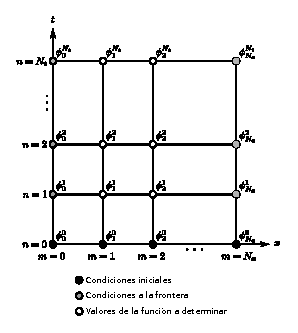
\includegraphics[height=11.5cm]{malla}
	\caption{Malla computacional.}
	\label{grid}
\end{figure}

Las FDF se obtienen a partir de la EDP del caso particular de estudio, haciendo expansiones en series de Taylor de la función alrededor de los puntos en la malla. Introducimos la notación $\phi^n_m=\phi(t=n\Delta t,x=m\Delta x)$ para simplificar las ecuaciones, y denotaremos simplemente como $(n,m)$ al punto $(t=n\Delta t, x=m\Delta x)$, de manera que el valor de la función $\phi$ alrededor del punto $(n+1,m)$ viene dado por
\begin{equation}
\phi^{n+1}_m=\phi^n_m+\left(\partial_t\phi\right)\Delta t+\mathcal{O}\{\left(\Delta t\right)^2\}
\end{equation}
y despejando se obtiene
\begin{equation}
\partial_t\phi\approx\frac{\phi^{n+1}_m-\phi^n_m}{\Delta t}
\label{timeapprox}
\end{equation}
Haciendo una expansión en series de Taylor alrededor de los puntos $(n,m-1)$, $(n,m)$ y $(n,m+1)$ se puede mostrar que
\begin{equation}
\partial_x\phi\approx\frac{\phi^n_{m+1}-\phi^n_{m-1}}{2\Delta x}
\label{spaceapprox}
\end{equation}
Algunas aproximaciones usadas comúnmente se muestran en la tabla \ref{aproxdiffin}. Así, substituyendo las ecuaciones \eqref{timeapprox} y \eqref{spaceapprox} en la ecuación \eqref{advection1d}, se obtiene la siguiente FDF para la ecuación de advección
\begin{equation}
\frac{\phi_m^{n+1}-\phi_m^n}{\Delta t}+\upsilon\left(\frac{\phi^n_{m+1}-\phi^n_{m-1}}{2\Delta x}\right)=0
\end{equation}
que puede reescribirse como
\begin{equation}
\phi_m^{n+1}=\phi_m^n-\frac{1}{2}\upsilon\rho\left(\phi^n_{m+1}-\phi^n_{m-1}\right)
\label{fdf}
\end{equation}
siendo $\rho$ el \textit{Factor de Courant}, definido como
\begin{equation}
\rho=\frac{\Delta t}{\Delta x}
\end{equation}
Las FDF's tales como la descrita en la ecuación \eqref{fdf}, se utilizan para determinar $\phi$ para un paso de tiempo $n+1$ a partir del valor de $\phi$ en el tiempo $n$, es por esto que se precisa conocer $\phi^0$ (es decir, tener una condición inicial) para poder comenzar la evolución.

 
\begin{table}[htb]
	\centering
	\caption{Fórmulas en diferencias finitas para primera y segunda derivada de una función $f$ respecto de una variable $u$, en una malla uniforme con espaciamiento $h$.}
	\label{aproxdiffin}
	{\tabulinesep=1.2mm
		\begin{tabu}{lc}
		\hline
		\multicolumn{1}{|c|}{\textbf{Primera derivada}}               														                 & \multicolumn{1}{c|}{\textbf{Error}}              \\ \hline
		\multicolumn{1}{|l|}{\(\displaystyle\partial_u f\simeq\frac{f_{i-2}-4f_{i-1}+3f_i}{2h}\)}                                            & \multicolumn{1}{l|}{\(\displaystyle\frac{1}{3}h^2 f^{(3)}\)}    \\ \hline
		\multicolumn{1}{|l|}{\(\displaystyle\partial_u f\simeq\frac{f_{i+1}-f_{i-1}}{2h}\)}                                                  & \multicolumn{1}{l|}{\(\displaystyle\frac{1}{6}h^2 f^{(3)}\)}    \\ \hline
		\multicolumn{1}{|l|}{\(\displaystyle\partial_u f\simeq\frac{-3f_{i}+4f_{i+1}-f_{i+2}}{2h}\)}                                         & \multicolumn{1}{l|}{\(\displaystyle\frac{1}{3}h^2 f^{(3)}\)}    \\ \hline
		\multicolumn{1}{|l|}{\(\displaystyle\partial_u f\simeq\frac{3f_{i-4}-16f_{i-3}+36f_{i-2}-48f_{i-1}+25f_i}{12h}\)}                    & \multicolumn{1}{l|}{\(\displaystyle\frac{1}{5}h^4f^{(5)}\)}     \\ \hline
		&                                                  \\ \hline
		\multicolumn{1}{|c|}{\textbf{Segunda derivada}}               																	     & \multicolumn{1}{c|}{\textbf{Error}}              \\ \hline
		\multicolumn{1}{|l|}{\(\displaystyle\partial^2_u f\simeq\frac{-f_{i-3}+4f_{i-2}-5f_{i-1}+2f_i}{h^2}\)}                               & \multicolumn{1}{l|}{\(\displaystyle\frac{11}{12}h^2f^{(4)}\)}   \\ \hline
		\multicolumn{1}{|l|}{\(\displaystyle\partial^2_u f\simeq\frac{f_{i-1}-2f_i+f_{i+1}}{h^2}\)}                                          & \multicolumn{1}{l|}{\(\displaystyle\frac{1}{12}h^2f^{(4)}\)}    \\ \hline
		\multicolumn{1}{|l|}{\(\displaystyle\partial^2_u f\simeq\frac{2f_i-5f_{i+1}+4f_{i+2}-f_{i+3}}{h^2}\)}                                & \multicolumn{1}{l|}{\(\displaystyle\frac{11}{12}h^2f^{(4)}\)}   \\ \hline
		\multicolumn{1}{|l|}{\(\displaystyle\partial^2_u f\simeq\frac{-10f_{i-5}+61f_{i-4}-156f_{i-3}+214f_{i-2}-154f_{i-1}+45f_i}{12h^2}\)} & \multicolumn{1}{l|}{\(\displaystyle\frac{137}{180}h^2f^{(6)}\)} \\ \hline
	\end{tabu}}
\end{table}

En dos dimensiones, la ecuación de advección es, considerando un campo escalar tal que $\phi=\phi(t,x,y)$,
\begin{equation}
\partial_t\phi+\upsilon_x\partial_x \phi+\upsilon_y\partial_y \phi=0
\label{advection2d}
\end{equation}
siendo $\upsilon_x$ y $\upsilon_y$ las velocidades en las direcciones de las coordenadas $x$ y $y$, respectivamente. La generalización de los MDF del caso unidimensional al caso bidimensional es inmediata.

\subsection{Consistencia, Estabilidad y Convergencia}\label{cec}
\noindent
En todo método numérico, es necesario conocer la precisión con la que las soluciones obtenidas por el método se acercan a la solución real, es decir, cuales son los errores introducidos por la aproximación. El análisis de consistencia, inestabilidad y convergencia de los métodos tienen este propósito. Para comenzar a analizar los errores en las aproximaciones en diferencias finitas, se escribe una ecuación diferencial de manera general como
\begin{equation}
\mathcal{L}\phi=0
\end{equation}
siendo $\phi$ un conjunto de funciones de las coordenadas espacio temporales $\left(t,\vec{x}\right)$ y $\mathcal{L}$ el operador diferencial que actúa sobre dichas funciones. Denotamos como $\phi_{\Delta}$ a la aproximación discretizada de $\phi$ evaluada en los puntos de la malla computacional y como $\mathcal{L}_{\Delta}$ a la versión en diferencias finitas del operador original. Así, la versión en diferencias finitas de una ecuación diferencial se escribiría
\begin{equation}
\mathcal{L}_{\Delta}\phi_{\Delta}=0
\end{equation}
haciendo así explícita la dependencia en $\Delta t$ y $\Delta x$ del esquema en diferencias finitas. Dado que se realiza una aproximación a una ecuación diferencial, el comportamiento de $\phi_{\Delta}$ es importante en el límite cuando $\Delta$ tiende a cero. Se define el error de truncado $\tau$ de la aproximación por diferencias finitas como
\begin{equation}
\tau_{\Delta}\coloneqq\mathcal{L}_{\Delta}\phi
\end{equation}
Un requisito mínimo para cualquier operador en diferencias finitas es que este error de truncado tienda a cero a medida que $\Delta x$ y $\Delta t$ disminuyan, lo que se conoce como refinamiento de la malla. Matemáticamente esto se representa como
\begin{equation}
\lim_{\Delta\rightarrow 0}\tau_{\Delta}=0
\end{equation}
De esta forma, al hacer una aproximación en diferencias finitas se busca que, en el límite continuo, estas tiendan a la ecuación diferencial original y no a una distinta. Cuando esto pasa localmente se dice que la aproximación es \textit{\textbf{consistente}}, y típicamente cuando esto sucede el error de truncamiento se acerca a cero como una potencia del parámetro de discretización $\Delta$. Se dice entonces que una cierta aproximación es de orden $n$ si
\begin{equation}
\lim_{\Delta\rightarrow 0}\tau_{\Delta}\sim\Delta^n
\end{equation}
Sin embargo, la consistencia es una propiedad local y en la práctica se requiere una propiedad que garantice que la aproximación numérica mejore después de un tiempo finito a medida que la malla se refine, es decir, que el error en la solución definido como
\begin{equation}
\epsilon_\Delta\coloneqq\phi-\phi_{\Delta}
\label{erroredf}
\end{equation} 
tienda a cero en el límite continuo después de un tiempo finito. A esta condición se le conoce como \textit{\textbf{convergencia}}.

Introducimos ahora la llamada norma $L^2$ de una aproximación en diferencias finitas como
\begin{equation}
\norm{\phi_{\Delta}^n}\coloneqq\left[\Delta x\ \sum_m \left|\left(\phi_{\Delta}\right)^n_m\right|^2\right]^{\frac{1}{2}}
\label{l2norm}
\end{equation}
donde la suma es sobre todos los puntos de la parte espacial de la malla. Se dice que una aproximación es \textit{\textbf{estable}} si para cualquier $t>0$ existe una constante $C_t$ tal que
\begin{equation}
\norm{\phi^n_\Delta}\leq C_t\norm{\phi^0_\Delta}
\end{equation}
para cualquier $0<n\Delta t<t$, en el límite cuando $\Delta x$ y $\Delta t$ tienden a cero. En otras palabras, que una aproximación sea estable significa que independientemente del comportamiento de la solución de la ecuación diferencial $\phi$, la solución exacta de las ecuaciones en diferencias finitas $\phi_\Delta$ debe permanecer acotada después de un tiempo finito $t$ para cualquier paso de tiempo $\Delta t$.

Relacionado a esto, se escribe el siguiente teorema esencial en la teoría de las aproximaciones en diferencias finitas\footnote{Ver \citet{alcubierre}, pp. 318-322.}:

\vspace{0.5cm}
\noindent
\textbf{\textit{Teorema de Equivalencia de Lax.}}	\textit{Dado un problema de valores iniciales que está matemáticamente bien definido, y una aproximación a este en diferencias finitas que es consistente, entonces la estabilidad de la aproximación es una condición necesaria y suficiente para garantizar la convergencia.}

\subsubsection{Análisis de Estabilidad de Von Neumann}
\noindent 
La estabilidad de una EDF se puede estudiar mediante el \textit{análisis de estabilidad de Von Neumann}\footnote{En esta sección solamente se describirán los pasos para el análisis, ver \citet{Hirsch2007} sección 7.2, para una justificación del método.}. Este método se basa en suponer un problema que posee condiciones a la frontera periódicas, además de estar restringido a problemas que son lineales. De esta forma, dado un esquema numérico lineal, se concluye que el error asociado al método numérico satisface la misma ecuación que la solución numérica. 

Posteriormente, se toma a la solución exacta de la ecuación en diferencias $\phi_i^n$ y se descompone en una serie de Fourier finita 
\begin{equation}
\phi_m^n=\sum_{j=-N}^{N}V_j^n\exp\left[i k_jm\Delta x\right]
\end{equation}
donde $i=\sqrt{-1}$ y $V_j^n$ es la amplitud de j-ésimo armónico. Esta descomposición separa la dependencia en el tiempo (dada por las amplitudes $V^n$) de la dependencia espacial (dada por los modos de Fourier). La estabilidad está descrita por la condición de que la amplitud de cualquier armónico no debe crecer indefinidamente en el tiempo, es decir, cuando $n$ tienda a infinito. Esto se mide definiendo el factor de amplificación 
\begin{equation}
G=\frac{V^{n+1}}{V^n}
\end{equation}

Los pasos para realizar el análisis, dado un cierto esquema numérico, son los siguientes:

\begin{enumerate}
	\item Se reemplazan todos los términos en la EDF de la forma $\phi^{n+k}_{p+m}$ de la siguiente manera
	\begin{equation}
	\phi^{n+k}_{p+m}\rightarrow V^{n+k}_j\exp\left[ik_j(p+m)\Delta x\right]
	\end{equation}
	\item Derivar una forma explícita para el factor de amplificación $G$.
	\item La estabilidad se obtiene de la siguiente condición
	\begin{equation}
	|G|\leq 1 \text{ para todos los valores de $k_j\Delta x$ con $j\in{-N,\dots,+N}$}
	\end{equation}
	donde $N$ es el número de espacios en los que se divide la malla del dominio espacial.
\end{enumerate}

La aproximación representada por la FDF escrita en la ecuación \eqref{fdf}, conocida como \textit{Método de Euler}, servirá para ejemplificar los pasos para el análisis de estabilidad de Von Neumann. Reescribimos dicha ecuación mostrando explícitamente el factor de Courant
\begin{equation}
\phi_m^{n+1}=\phi^n_m-\frac{\upsilon\Delta t}{2\Delta x}\left(\phi_{m+1}^n-\phi_{m-1}^n\right)
\label{euler}
\end{equation}
Consideramos un  modo de Fourier de la forma
\begin{equation}
\phi^n_m=V^n\text{e}^{imk\Delta x}
\end{equation}
y sustituyendo esta expresión en la ecuación \eqref{euler}, se obtiene que
\begin{align}
V^{n+1}\text{e}^{ikm\Delta x}=V^n\text{e}^{ikm\Delta x}-\frac{\upsilon \Delta t}{2\Delta x}\left(V^n\text{e}^{ik(m+1)\Delta x}-V^n\text{e}^{ik(m-1)\Delta x}\right)
\end{align}
dividiendo la última ecuación entre $V^n\text{e}^{ikm\Delta x}$, se obtiene
\begin{align}
G=1-\frac{\upsilon\Delta t}{2\Delta x}\left(\text{e}^{ik\Delta x}-\text{e}^{-ik\Delta x}\right)
\end{align}
Para que el sistema sea estable se debe pedir que $\left|G\right|\leq 1$, sin embargo, se observa que
\begin{equation}
\left|G\right|^2=1+\upsilon^2\left(\frac{\Delta t}{\Delta x}\right)^2\sin^2\left(k\Delta x\right)
\end{equation}
ocasionando que $\left|G\right|\geq 1$ para cualquier $k$, por lo que se concluye que el sistema es incondicionalmente inestable, es decir, inestable para cualquier elección de $\Delta t$ y $\Delta x$.

Un método a segundo orden tanto en tiempo como en espacio se obtiene al expandir en una serie de Taylor truncándola hasta segundo orden
\begin{equation}
\phi^{n+1}_m=\phi_m^n+\Delta t\ \partial_t \phi+\frac{\left(\Delta_t t\right)^2}{2}\ \partial^2\phi+\dots
\end{equation}
y recordando la ecuación de advección $\partial_t\phi=-\upsilon\ \partial_x\phi$, lo anterior se reescribe como
\begin{equation}
\phi^{n+1}_m=\phi^n_m-\upsilon\ \Delta t\ \partial_x \phi+\upsilon^2\frac{\left(\Delta t\right)^2}{2}\partial_x^2\phi+\dots
\end{equation}
y aproximando las derivadas espaciales por derivadas centradas se obtiene la aproximación en diferencias finitas conocida como de \textit{Lax-Wendroff}\footnote{Se tratará más acerca de esta aproximación posteriormente, ya que, junto con la aproximación de \textit{upwind a primer orden}, es la base del método limitador de flujo que se presenta en la sección \ref{limflujo}.}
\begin{equation}
\phi^{n+1}_m=\phi^n_m-\frac{\upsilon \rho}{2}\left(\phi_{m+1}^n-\phi_{m-1}^n\right)+\frac{\upsilon^2\rho^2}{2}\left(\phi^n_{m+1}-2\phi^n_m+\phi^n_{m-1}\right)
\end{equation}
Haciendo un análisis de estabilidad de Von Neumann con un modo de Fourier $\phi^n_m=V^ne^{imk\Delta x}$ se encuentra que
\begin{equation}
G=1-i\upsilon\rho\sin\left(k\ \Delta x\right)+\upsilon^2\rho^2\left(\cos\left(k\ \Delta x\right)-1\right)
\end{equation}
e imponiendo $\left|G\right|\leq 1$, se obtiene la condición de estabilidad
\begin{equation}
\upsilon\rho\leq 1
\end{equation}
Esta última relación se conoce como condición estándar de \textit{Courant-Friederich-Lewy} (CFL), y se puede interpretar de manera geométrica como que el dominio de dependencia numérico debe ser más grande que el dominio de dependencia física. 

El esquema de Lax-Wendroff en dos dimensiones se escribe de la siguiente manera
\begin{eqnarray}
\nonumber
\phi^{n+1}_{j,k}=\phi^n_{j,k}&-\frac{\upsilon_x \rho_x}{2}\left(\phi_{j+1,k}^n-\phi_{j-1,k}^n\right)+\frac{\upsilon_x^2\rho_x^2}{2}\left(\phi^n_{j+1,k}-2\phi^n_{j,k}+\phi^n_{j-1,k}\right)\\
&-\frac{\upsilon_y \rho_y}{2}\left(\phi_{j,k+1}^n-\phi_{j,k-1}^n\right)+\frac{\upsilon_y^2\rho_y^2}{2}\left(\phi^n_{j,k+1}-2\phi^n_{j,k}+\phi^n_{j,k-1}\right)
\end{eqnarray}
El análisis de estabilidad de Von Neumann para este esquema se realiza usando un modo de Fourier de la forma
\begin{equation}
\phi^n_{j,k}=V^n\text{e}^{i\left(j\xi\Delta x+k\eta\Delta y\right)}
\end{equation}
de donde se deduce que la condición de estabilidad es
\begin{equation}
\text{max}\left\{\upsilon_x \rho_x,\ \upsilon_y\rho_y\right\}\leq \frac{1}{\sqrt{2}}
\label{cfl}
\end{equation}
siendo $\upsilon_x$ y $\upsilon_y$ las velocidades en las direcciones de las coordenadas $x$ y $y$, respectivamente\footnote{Ver \citet{Thomas1998}, sección 5.8.}.

\section{Leyes de Conservación}\label{sec:leyesdeconservacion}
%%%%%%%%%%%%%%%%%%% Revisar, copiado prácticamente del Leveque %%%%%%%%%%%%%%%%%%%
\noindent
Se considerará un caso simple con el propósito de ilustrar cómo las leyes de conservación surgen a partir de principios físicos. Consideremos el caso de un gas o un líquido que fluye a través de un tubo unidimensional con una velocidad conocida $u(x,t)$. Típicamente, en los problemas de dinámica de fluidos, se espera encontrar esta velocidad $u$ como parte de la solución, sin embargo, en este momento se toma por conocida. En este ejemplo solo se busca modelar la densidad de un cierto químico en el fluido; sea $\phi(x,t)$ la densidad de este elemento químico, siendo esta la función a determinar.

Esta densidad, dado que se está trabajando en un problema unidimensional, tiene unidades de masa por unidad de longitud, y puede obtenerse multiplicando la función de densidad tridimensional por el área de la sección transversal del tubo. Así, la ecuación
\begin{equation}
\int_{x_1}^{x_2}\phi(x,t)\ \text{d}x
\end{equation} 
representa la masa total del químico en la sección del tubo que va de $x_1$ a $x_2$ al tiempo $t$. Consideremos una sección del tubo comprendida en $x_1<x<x_2$ y la manera en que la integral anterior cambia con el tiempo. Suponiendo que la sustancia no se crea ni se destruye dentro de esta sección, entonces la masa total en dicha sección puede cambiar únicamente por el flujo de partículas a través de los extremos de esta sección, ubicados en $x_1$ y $x_2$. Sea $F_i(t)$ la velocidad con la que el químico fluye a través de los extremos $x_i$, con $i=1,2$. Dado que la masa total en la sección que estamos considerando sólo cambia por los flujos en los extremos, entonces
\begin{equation}
\frac{\text{d}}{\text{d}t}\int_{x_1}^{x_2}\phi(x,t)\ \text{d}x=F_1(t)-F_2(t)
\label{intformconservation}
\end{equation}

La ecuación \ref{intformconservation} es la forma integral de una ley de conservación. Es necesario determinar cómo las funciones de flujo $F_j(t)$ se relacionan con $\phi(x,t)$, para poder obtener una ecuación que pueda resolverse para $q$. En el caso del fluido considerado en este ejemplo, el flujo $f$ en cualquier punto $x$ al tiempo $t$ esta dado simplemente por el producto de la densidad $\phi(x,t)$ y la velocidad $u(x,t)$ del mismo
\begin{equation}
f(x,t)=u(x,t)\ \phi(x,t)
\end{equation}

El flujo mide la velocidad a la cual la sustancia pasa a través del extremo de la sección del tubo estudiada. Dado que se tiene a $u(x,t)$ como una función conocida, entonces es posible escribir la función del flujo $f$ como
\begin{eqnarray}
f(\phi,x,t)=u(x,t)\ \phi(x,t)
\end{eqnarray} 

En particular, si se supone que la velocidad es independiente de $x$ y de $t$, de tal forma que $u(x,t)=u$ sea una constante, entonces se puede escribir
\begin{equation}
f(\phi)=u\phi
\end{equation}
En este caso, el flujo en cualquier punto y a cualquier tiempo se puede determinar directamente con el valor de la cantidad conservada en ese punto, y no depende de la posición del punto en el espacio-tiempo. En este caso, la ecuación se conoce como \textit{autónoma}.

Para un flujo autónomo $f(\phi)$ que depende únicamente del valor de $\phi$, la ley de conservación \ref{intformconservation} se puede reescribir como
\begin{equation}
\frac{\text{d}}{\text{d}t}\int_{x_1}^{x_2}\phi(x,t)\ \text{d}x=f(\phi(x_1,t))-f(\phi(x_2,t))=-\left.f(\phi(x,t))\right|_{x_1}^{x_2}
\end{equation} 

\noindent
y dado que ya se conoce la forma de $f$, se tiene entonces una ecuación para $\phi$. Esta ecuación debe valer para cualquier intervalo $\left[x_1,x_2\right]$ para valores arbitrarios de $x_1$ y $x_2$. Transformamos esta ecuación de manera que obtengamos una ecuación diferencial parcial, para esto, se supone que las funciones $\phi(x,t)$ y $f(\phi)$ son suficientemente suaves. Tomando en cuenta esto último, la última ecuación se puede escribir como
\begin{equation}
\frac{\text{d}}{\text{d}t}\int_{x_1}^{x_2}\phi(x,t)\ \text{d}x=-\int_{x_1}^{x_2}\frac{\partial}{\partial x}f(\phi(x,t))\ \text{d}x
\end{equation}
y reordenando
\begin{equation}
\int_{x_1}^{x_2}\left[\frac{\partial}{\partial t}\phi(x,t)+\frac{\partial}{\partial x}f(\phi(x,t))\right]\ \text{d}x=0
\end{equation}
Dado que esta integral debe ser cero para todos los valores de $x_1$ y $x_2$, se sigue que el integrando debe ser idénticamente cero, lo que da finalmente la ecuación diferencial
\begin{equation}
\frac{\partial}{\partial t}\phi(x,t)+\frac{\partial}{\partial x}f(\phi(x,t))=0
\end{equation}
A esta ecuación se le conoce como la forma diferencial de las leyes de conservación.

La anterior ecuación vale para una dimensión. En el caso multidimensional, se debe considerar un dominio espacial arbitrario $\Omega$ sobre el cual se asume que $\phi$ se conserva, por lo que la integral de $\phi$ sobre $\Omega$ varía únicamente debido al flujo que pasa a través de la frontera de $\Omega$, a esta última la denotamos $\partial\Omega$. Así, se tiene lo siguiente
\begin{equation}
\frac{\text{d}}{\text{d}t}\int\int_\Omega \phi(x,y,t)\ \text{d}x\ \text{d}y=\ \mathbf{Flujo\ neto\ que\ pasa\ por\ }\partial\Omega
\label{flujo2d}
\end{equation}
El flujo neto se determina integrando el flujo de $\phi$ normal a $\partial\Omega$ alrededor de la frontera.

Sea $f(\phi)$ el flujo de $\phi$ en la dirección $x$. Esto quiere decir que el flujo total a través del intervalo que va de $(x_0,y_0)$ a $(x_0,y_0+\Delta y)$ en el tiempo $\Delta t$ es ($\Delta t\ \Delta y \ f(\phi(x_0,y_0))$) para $\Delta t$ y $\Delta y$ suficientemente pequeñas\footnote{Ver \citet{leveque}.}.

Análogamente, sea $g(\phi)$ el flujo en la dirección $y$, y sea $\vec{f}(\phi)=(f(\phi),g(\phi))$ el vector de flujo. Sea $\vec{n}(s)=\left(n^x(s),n^y(s)\right)$ un vector unitario normal que apunta hacia afuera de $\partial\Omega$ en el punto $(x(s),y(s))$ contenido en $\partial\Omega$, siendo $s$ la longitud de arco que parametriza $\partial\Omega$. De esta forma, el flujo en $\vec{x}=(x(s),y(s))$ en la dirección $\vec{n}(s)$ es
\begin{equation}
\vec{n}(s)\cdot\vec{f}\left(\phi(x(s),y(s),t)\right)=n^x(s)f(\phi)+n^y(s)g(\phi)
\end{equation}
Así, la ecuación \ref{flujo2d} se convierte
\begin{equation}
\frac{\text{d}}{\text{d}t}\int\int_\Omega \phi(x,y,t)\ \text{d}x\ \text{d}y=-\int_{\partial\Omega}\vec{n}\cdot\vec{f}(\phi)\ \text{d}s
\end{equation}
Suponiendo que $\phi$ es suave, es posible usar el Teorema de la Divergencia para escribir esta última ecuación como
\begin{equation}
\frac{\text{d}}{\text{d}t}\int\int_\Omega \phi(x,y,t)\ \text{d}x\ \text{d}y=-\int\int_{\Omega}\nabla\cdot\vec{f}(\phi)\ \text{d}x\ \text{d}y
\end{equation}
de donde se obtiene finalmente
\begin{equation}
\int\int_{\Omega}\left[\frac{\partial}{\partial t}\phi+\nabla\cdot\vec{f}(\phi)\right]\ \text{d}x\ \text{d}y=0
\end{equation}
y dado que esto se debe cumplir para cualquier región $\Omega$, el integrando debe ser cero, por lo que se obtiene una ley de conservación en forma diferencial. El argumento se realizó para el caso bidimensional pero se puede extender al caso de $n$ dimensiones de manera inmediata.

En particular, en dos dimensiones una ley de conservación toma la forma
\begin{equation}
\partial_t \phi+\frac{\partial}{\partial x}f\left(\phi(x,y,t)\right)+\frac{\partial}{\partial y}g\left(\phi(x,y,t)\right)=0
\label{conserv2D}
\end{equation}

Se puede observar que la ecuación \eqref{advection2d} puede verse como una ley de conservación si se cumple que $f(\phi)=\upsilon_x\phi$, $g(\phi)=\upsilon_y\phi$ y además $\frac{\partial \upsilon_x}{\partial x}=\frac{\partial\upsilon_y}{\partial y}=0$. Bajo estás condiciones, la ecuación de advección 2-dimensional se reescribe
\begin{equation}
\partial_t \phi+\partial_x\left(\upsilon_x \phi\right)+\partial_y \left(\upsilon_y \phi\right)=0
\label{adv2d}
\end{equation}

\subsection{Métodos Conservativos}
\noindent
Cuando se busca resolver leyes de conservación no lineales por métodos numéricos se pueden encontrar problemas que no surgen en el caso lineal, uno de dichos problemas es que el método puede converger a una función que no es una solución débil\footnote{La formulación débil de una ecuación diferencial es aquella en la que no aparecen derivadas de la solución. De esta manera, una solución débil es aquella que satisface la formulación débil. En otras palabras, esta solución requiere menos condiciones de suavidad para cumplir con la ecuación diferencial original. Ver \citet{levequenmcl}, capítulos 3 y 12.} de la ecuación diferencial original. Un requerimiento que garantiza evitar este problema es que el método numérico esté escrito en forma conservativa, es decir, que tenga la siguiente forma 
\begin{equation}
\phi_j^{n+1}=\phi_j^n -\frac{\Delta t}{\Delta x}\left[\mathcal{F}\left(\phi_{j-p}^n,\phi_{j-p+1},\dots,\phi^n_{j+q}\right)-\mathcal{F}\left(\phi^n_{j-p-1},\phi^n_{j-p},\dots,\phi^n_{j+q-1}\right)\right]
\label{conservativeform}
\end{equation}
para alguna función $\mathcal{F}$ de $p+q+1$ argumentos. A la función $\mathcal{F}$ se le conoce como la \textit{función de flujo numérico}. En el caso más simple, $p=0$ y $q=1$ de manera que $\mathcal{F}$ es solo función de dos variables, por lo que la ecuación \eqref{conservativeform} se vuelve
\begin{equation}
\phi_{j}^{n+1}=\phi_j^n-\frac{\Delta t}{\Delta x}\left[\mathcal{F}\left(\phi_j^n,\phi_{j+1}^n\right)- \mathcal{F}\left(\phi_{j-1}^n,\phi_j^n\right)\right]
\end{equation}

La función de flujo numérico $\mathcal{F}\left(\phi_j,\phi_{j+1}\right)$ representa un flujo promedio que pasa a través de $x_{j+1/2}$ en el intervalo de tiempo $\left[t_n,t_{n+1}\right]$ representado como
\begin{equation}
\mathcal{F}\left(\phi_j,\phi_{j+1}\right)\sim\frac{1}{\Delta t}\int_{t_n}^{t_{n+1}}f\left(\hat{\phi}\left(x_{j+1/2},t\right)\right)\ \text{d}t
\end{equation} 
donde $\hat{\phi}(x,t)$ denota la solución débil de la ecuación diferencial, y $f(\hat{\phi})$ denota una función adecuada de dicha solución. La forma de derivar métodos numéricos en su forma conservativa es encontrar las aproximaciones en diferencias finitas de la forma estándar vista anteriormente, pero partiendo de la forma conservativa de la EDP que se esté estudiando\footnote{Ver \citet[pág. 124-125]{levequenmcl}.}.

\section{Métodos de Alta Resolución}
\noindent
Cuando se quiere resolver un problema vía un método numérico asumiendo que las soluciones son suaves, se pueden esperar complicaciones debidas principalmente a que, cerca de discontinuidades, la EDP no se cumple. Esto ocasiona, en el caso de métodos de primer orden, que la solución numérica se ``suavice'' cerca de discontinuidades (a este comportamiento se le conoce como ''viscosidad numérica''). En cambio, para los métodos de segundo orden, se logra eliminar dicha viscosidad numérica, pero se introducen efectos dispersivos que dan lugar a oscilaciones muy grandes en la solución numérica\footnote{En la sección \ref{pruebascasoparticular} se trata un caso en el que se pueden ver estos efectos gráficamente.}. Para resolver este tipo de inconvenientes, se recurre a los métodos de ``alta resolución'', los cuales tienen las siguientes propiedades:
\begin{itemize}
	\item En su parte espacial tienen una precisión de orden dos o mayor alrededor de partes suaves de la solución.
	\item Las soluciones no presentan oscilaciones espurias.
	\item Se obtiene una gran precisión alrededor de choques o discontinuidades.
\end{itemize}

\begin{comment}
\begin{figure}[h!]
\centering
\includegraphics[height=7cm]{comparacion.png}
\caption{Imagen obtenida de \citet[pág. 10]{levequenmcl}, en ella se muestran las diferencias entre el perfil de densidad real (imagen superior izquierda) y una aproximación por un método numérico de primer orden (imagen superior derecha), de segundo orden (imagen inferior izquierda) y uno de alta resolución (imagen inferior derecha).}
\label{comparacion}
\end{figure}
\end{comment}

Para resolver la ecuación de Vlasov, lo que se busca es encontrar la forma en la que evoluciona la función de distribución, la cuál es siempre positiva. Debido a esto último, se requiere que el método utilizado preserve la monotonía de los datos iniciales durante la evolución, es decir, evitando oscilaciones espurias, y por ello recurrimos a los métodos de alta resolución. Sin embargo, Godunov demostró que un método lineal y que preserve la monotonía es a lo más de primer orden\footnote{Para una demostración de este teorema ver \citet{levequenmcl}, pp. 174-175.}, por lo que se deben construir métodos no lineales para obtener una precisión de segundo orden y que preserve la monotonía de la solución. Algunos de los métodos que poseen estas características se conocen como \textit{limitadores de flujo}.

\subsection{Limitadores de Flujo}\label{limflujo}
\noindent
La idea básica de este tipo de métodos es utilizar un flujo de orden alto $\mathcal{F}_H$ en regiones suaves y uno de orden bajo $\mathcal{F}_L$ que preserve la monotonicidad de la función cerca de una discontinuidad. Escribimos el flujo total $\mathcal{F}$ de la siguiente manera
\begin{equation}
\mathcal{F}=\mathcal{F}_H-\left(1-\Psi\right)\left(\mathcal{F}_H-\mathcal{F}_L\right)
\label{flujototal}
\end{equation}
donde a $\Psi$ se le conoce como el \textit{limitador}, que debe tender a uno si la región de la solución es suave y debe tender a cero si está cerca de una discontinuidad. Para medir la ``suavidad'' de la solución se puede analizar el radio entre gradientes consecutivos; denotando $\phi_j$ como la parte puramente espacial de un punto de la malla computacional, vemos a este radio como
\begin{equation}
\theta_j=\frac{\phi_j-\phi_{j-1}}{\phi_{j+1}-\phi_j}
\end{equation}
Se toma entonces a $\Psi_j$ como una función de $\theta_j$, de manera que
\begin{equation}
\Psi_j=\Psi_j\left(\theta_j\right)
\end{equation} 
Existen varias posibilidades para elegir estos limitadores dados en la literatura, y en este trabajo se analizan las siguientes
\begin{itemize}
	\item \textbf{Minmod}
	\begin{equation}
	\Psi\left(\theta\right)=\text{max}\left[0,\text{min}(1,\theta)\right]
	\end{equation}
	\item \textbf{Superbee}
	\begin{equation}
	\Psi\left(\theta\right)=\text{max}\left[0,\text{min}\left(1,2\theta\right),\text{min}\left(\theta,2\right)\right]
	\end{equation}
	\item \textbf{Monotonized Central}
	\begin{equation}
	\Psi\left(\theta\right)=\text{max}\left[0,\text{min}\left(2\theta,\frac{1}{2}\left(1+\theta\right),2\right)\right]
	\end{equation}
\end{itemize}

Los limitadores son iguales a cero cuando se encuentran en un extremo local, lo que significa que los métodos se reducen a primer orden en esos lugares. Los limitadores son construidos de manera que la variación total de la solución numérica nunca aumente. Esta variación se define como
\begin{equation}
TV(\phi)\coloneqq\sum_{m}\left|\phi_m-\phi_{m-1}\right|
\end{equation} 
Los métodos que satisfacen esta propiedad se dice que disminuyen la variación total y se conocen por su traducción al inglés como TVD (\textit{Total Variation Diminishing}). Por definición, estos métodos no generan oscilaciones espurias, ya que de otra forma incrementarían la variación total.

\section{Método de Líneas}
\noindent
El método de líneas se basa en separar la discretización espacial de la discretización temporal, lo que nos permite utilizar cualquier método para resolver ecuaciones diferenciales ordinarias para ambas partes, por lo que se puede elegir el orden de convergencia de dichas partes de manera que no dependan una de otra. Para esto, se procede primero discretizando las dimensiones espaciales dejando la parte temporal continua. Se comienza escribiendo la ecuación diferencial parcial como
\begin{equation}
\partial_t\phi=\mathrm{S}\left(\phi\right)
\end{equation} 
siendo $S$ un operador diferencial en el espacio. Usando un método en diferencias finitas, obtenemos un sistema acoplado de ecuaciones diferenciales ordinarias de la forma
\begin{equation}
\frac{\text{\textbf{d}}\boldmath{\phi}}{\text{\textbf{d}}t}=\boldmath{S}\boldmath{\phi}
\end{equation}
donde $\boldmath{\phi}$ es un vector que denota los valores de la función $\phi$ en los puntos espaciales de la malla, y $\boldmath{S}$ es una matriz que acopla los diferentes puntos en la malla.

Para ilustrar este método, se retoma el ejemplo de la ecuación de advección, donde se discretiza la parte espacial usando derivadas centradas
\begin{equation}
\frac{\text{d}\phi_m}{\text{d}t}=-\frac{u}{2\Delta x}\left(\phi_{m+1}-\phi_{m-1}\right)
\end{equation}
Una aproximación a primer orden en $\Delta t$ da el método de Euler mencionado anteriormente
\begin{eqnarray}
\frac{\text{d}\phi}{\text{d}t}=\mathrm{S}\left(\phi\right)\\
\phi_m^{n+1}=\phi_m^n+\Delta t\ \mathrm{S}\left(\phi^n\right)
\end{eqnarray}
método que ya se demostró en la sección \ref{cec}, es incondicionalmente inestable.

Un mejor método es el conocido como \textit{Runge-Kutta de orden 4}, que consiste en calcular recursivamente las cantidades
\begin{align*}
k_1&=\mathrm{S}\left(\phi^n\right)\\
k_2&=\mathrm{S}\left(\phi^n+k_1\ \Delta t/2\right)\\
k_3&=\mathrm{S}\left(\phi^n+k_2\ \Delta t/2\right)\\
k_4&=\mathrm{S}\left(\phi^n+k_3\ \Delta t\right)\\
\end{align*}
y luego tomar
\begin{equation}
\phi^{n+1}=\phi^n+\frac{\Delta t}{6}\left(k_1+2k_2+2k_3+k_4\right)
\end{equation}
Este método da una precisión de cuarto orden en el tiempo y es estable mientras se satisfaga la condición CFL, es este método el que se utiliza en este trabajo.
\begin{comment}
El método utilizado en este trabajo es el conocido como \textit{Crank-Nicholson Iterado} (ICN), cuya idea es tomar un esquema iterativo para aproximar la solución al esquema estándar de Crank-Nicholson descrito por \eqref{cn}. Visto como un método de líneas, dicha iteración se escribe como
\begin{align}
\phi^{*(1)}&=\phi^n+\Delta t\ \mathrm{S}\left(\phi^n\right)\\
\phi^{*(p)}&=\phi^n+\frac{\Delta t}{2}\left[\mathrm{S}\left(\phi^n\right)+\mathrm{S}\left(\phi^{*\left(p-1\right)}\right)\right], \hspace{0.5cm}p=2,\dots,N\\
\phi^{n+1}&=\phi^{*\left(N\right)} 
\end{align}
con $N\geq 2$. Este método toma como paso inicial el método de Euler, el cual aproxima la función al siguiente paso de tiempo y luego hace una iteración promediando las funciones del paso de tiempo anterior y la última aproximación del último paso de tiempo. Cuando las iteraciones convergen en el límite $N\rightarrow \infty$ se recupera el método de Crank-Nicholson visto en $\eqref{cn}$
\begin{equation}
\frac{\phi^{n+1}-\phi^n}{\Delta t}=\frac{1}{2}\left[\mathrm{S}\left(\phi^n\right)+\mathrm{S}\left(\phi^{n+1}\right)\right]
\end{equation} 
Para funciones fuentes lineales, las iteraciones se pueden escribir como
\begin{align}
\bar{\phi}^{*\left(p\right)}&=\phi^n+\frac{\Delta t}{2}\ \mathrm{S}\left(\bar{\phi}^{*\left(p-1\right)}\right),\hspace{0.5cm}p=1,\dots,N-1\\
\phi^{n+1}&=\phi^n+\Delta t\ \mathrm{S}\left(\bar{\phi}^{*\left(N-1\right)}\right)
\end{align}
con $\bar{\phi}^{*\left(p\right)}=\left(\phi^n-\phi^{*\left(p\right)}\right)$. Para sistemas lineales, ICN tiene las siguientes propiedades.
\begin{itemize}
	\item Para obtener un esquema estable se tiene que tomar al menos tres pasos, es decir, $N\geq 3$. La estabilidad viene en pares en términos del número de pasos: uno y dos pasos son inestables, tres y cuatro son estables, cinco y seis son inestables, etc.
	\item El esquema iterativo es solo convergente si la condición CFL estándar se satisface, en caso contrario las iteraciones divergen.
\end{itemize}

Así, se puede concluir que el tomar tres iteraciones basta para obtener un sistema estable mientras se satisfaga la condición CFL, además de que se llega a una precisión de segundo orden en el tiempo
\citet[pág. 339-343]{alcubierre}.
\end{comment}
\section{Análisis de convergencia y estabilidad}
\noindent
En todo problema numérico es necesario conocer si los cálculos realizados por la computadora se asemejan a la solución correcta. Para esto lo que se debe hacer es cuantificar el error de la aproximación numérica mediante una \textit{prueba de convergencia}, que nos permite conocer cuantitativamente el comportamiento del error. 

En principio, se supone que la solución a una aproximación estable en diferencias finitas puede interpretarse como una función continua que se puede expandir en series de potencias del parámetro de discretización $\Delta$ de la siguiente forma
\begin{equation}
u_{\Delta}\left(t,x\right)=u\left(t,x\right)+\Delta e_1\left(t,x\right)+\Delta^2 e_2\left(t,x\right)+\dots
\end{equation}
siendo $u\left(t,x\right)$ la solución original de la ecuación diferencial y $e_i\left(t,x\right)$ el error a orden $i$ de $\Delta$. Una aproximación es de orden $n$ si $e_i\left(t,x\right)=0,\ \forall i<n$.

Suponiendo que se conoce la solución exacta del problema que se esté estudiando, para probar la convergencia de la aproximación en diferencias finitas se realiza un cálculo a dos diferentes resoluciones $\Delta_1$ y $\Delta_2$, con $r\equiv\Delta_1/\Delta_2>1$, y se obtiene el error en la solución en cada caso
\begin{equation}
\epsilon_{\Delta_1}=u-u_{\Delta_1}, \hspace{1cm}\epsilon_{\Delta_2}=u-u_{\Delta_2}
\end{equation} 
Posteriormente se obtiene la norma $L^2$ \eqref{l2norm} para cada error, y se calcula el radio de ambas normas
\begin{equation}
c(t)\coloneqq\frac{\norm{\epsilon_{\Delta_1}}}{\norm{\epsilon_{\Delta_2}}}
\end{equation}
A este radio se le conoce como el \textit{factor de convergencia}. Si se tiene una aproximación en diferencias finitas de orden $n$, en el límite continuo debe suceder
\begin{equation}
\lim_{\Delta\rightarrow 0}c(t)=\left(\frac{\Delta_1}{\Delta_2}\right)^n=r^n
\end{equation}
De esta forma, si sucede que $c(t)$ se acerca al valor esperado (típicamente se toma $r=2$) se dice que se está en el régimen de convergencia.

Sin embargo, lo anterior funciona únicamente cuando se conoce la solución exacta del problema. Para los casos en los que no sucede esto (que son la mayoría) lo que se espera es probar que la solución numérica converja a alguna función continua. Para esto se requieren al menos tres diferentes resoluciones $\Delta_1>\Delta_2>\Delta_3$, se calculan los errores relativos entre las diferentes resoluciones, y se define el factor de convergencia como
\begin{equation}
c(t)\coloneqq\frac{\norm{u_{\Delta_1}-u_{\Delta_2}}}{\norm{u_{\Delta_2}-u_{\Delta_3}}}
\end{equation}
Nuevamente, en el límite continuo, se espera que el factor de convergencia se comporte como
\begin{equation}
\lim_{\Delta\rightarrow 0} c(t)=\frac{\Delta_1^n-\Delta_2^n}{\Delta_2^n-\Delta_3^n}
\end{equation}
y tomando $\Delta_1/\Delta_2=\Delta_2/\Delta_3\equiv r$, entonces
\begin{equation}
\lim_{\Delta\rightarrow 0}c(t)=r^n
\end{equation}
Debido a que se calculan normas de los errores, el análisis de convergencia es global. Para realizar un análisis local, se puede graficar los errores relativos $u_{\Delta_1}-u_{\Delta_2}$ y $u_{\Delta_2}-u_{\Delta_3}$ como funciones de la posición para poder compararlas cualitativamente. Como debe suceder que para un esquema de diferencias finitas de orden $n$ estos errores sean proporcionales a $e_n(t,x)$, se espera que si los errores relativos se reescalan apropiadamente, si se multiplica a $u_{\Delta_2}-u_{\Delta_3}$ por $r^n$, la gráfica debería de coincidir de manera aproximada con $u_{\Delta_1}-u_{\Delta_2}$\footnote{Ver \citet{alcubierre}, pp. 353-355.}.

Como ya se mencionó en la sección \ref{sec:: Teo virial}, el análisis de estabilidad se realizó con el teorema del Virial haciendo una aproximación Newtoniana.

\section{Métodos para la Ecuación de Advección}\label{pruebascasoparticular}
\noindent
Para probar los métodos empleados, se utilizó la siguiente solución conocida a la ecuación de advección bidimensional dada una condición inicial y ciertas velocidades: Sea un espacio de dos dimensiones espaciales $x$ y $y$, constantes dadas $m$, $a_x$, $a_y$, y campos de velocidades definidos como
\begin{align*}
u_x(x)=m(x+a_x),\hspace{1cm} u_y(y)=-m(y+a_y)
\end{align*}
para los cuales, la ecuación de advección bidimensional toma la forma siguiente
\begin{equation}
\partial_t f+u_x\ \partial_x f+u_y\ \partial_y f=\partial_t f+\partial_x\bigg(u_x\ f\bigg)+\partial_y\bigg(u_y\ f\bigg)=0
\end{equation}
donde se usó que los términos que incluyen las derivadas de los campos de velocidades se cancelan entre sí, por lo que generan un esquema conservativo, es decir
\begin{equation}
\partial_x u_x+\partial_y u_y=m+(-m)=0
\end{equation}
La anterior ecuación diferencial tiene la siguiente solución exacta\footnote{Solución obtenida usando un caso particular de la ecuación de advección en dos dimensiones sugerido en \citet{schullenfdmfaivvf}, con una ligera modificación para generar una ecuación conservativa. Este artículo estudia diferentes tipos de esquemas en diferencias finitas cambiando el factor de Courant, y el autor concluye que dichos esquemas generan resultados pobres aún siendo estables, sin embargo, ninguno de los métodos estudiados son de alta resolución como en el presente trabajo.}
\begin{equation}
f(t,x,y)=e^{-k_x\left[(x+a_x)e^{-m t}-x_0-a_x\right]^2} e^{-k_y\left[(y+a_y)e^{m t}-y_0-a_y\right]^2}
\end{equation}

A continuación se resumen los métodos utilizados en este trabajo para analizar la ecuación de Vlasov que, como ya se mencionó, es un caso especial de la ecuación de advección. Para obtener las gráficas mostradas en las figuras \ref{upwind1}-\ref{mc}, se utilizó el problema descrito arriba, mismo que permite dar una idea general de los resultados numéricos que se pueden esperar. 

Se escribe la ecuación de advección en una dimensión
\begin{equation}
\partial_t\phi+\upsilon\partial_x \phi=0
\end{equation}
donde $\phi$ es la solución de la ecuación y representa una onda, y $\upsilon$ es la velocidad con la que se propaga dicha onda. Los métodos que se describirán aquí mediante sus FDF son fáciles de extender al caso en dos dimensiones.

\begin{itemize}
	\item \textbf{Upwind de primer orden}
	\begin{align}
	\phi^{n+1}_m&=\phi^n_m-\upsilon\rho\left(\phi_m^n-\phi^n_{m-1}\right),\hspace{1cm}\upsilon>0\\
	\nonumber
	&\\
	\phi^{n+1}_m&=\phi^n_m-\upsilon\rho\left(\phi_{m+1}^n-\phi^n_{m}\right),\hspace{1cm}\upsilon<0
	\end{align}
	Este método es estable mientras se cumpla la condición CFL y es de primer orden tanto en espacio como en tiempo. Ver figura \ref{upwind1}.
	
	\item \textbf{Upwind de segundo orden}
	\begin{align}
	\phi^{n+1}_m&=\phi^n_m-\frac{\upsilon}{2}\rho\left(3\phi_m^n-4\phi_{m-1}^n+\phi_{m-2}^n\right),\hspace{1cm}\upsilon>0\\
	\nonumber
	&\\
	\phi^{n+1}_m&=\phi^n_m-\frac{\upsilon}{2}\rho\left(-\phi_{m+1}^n+4\phi_{m+1}^n-3\phi_m^n\right),\hspace{1cm}\upsilon<0
	\end{align}
	Ver figura \ref{upwind2}.
	
	\item \textbf{Lax-Wendroff}
	\begin{equation}
	\phi^{n+1}_m=\phi^n_m-\frac{\upsilon \rho}{2}\left(\phi_{m+1}^n-\phi_{m-1}^n\right)+\frac{\upsilon^2\rho^2}{2}\left(\phi^n_{m+1}-2\phi^n_m+\phi^n_{m-1}\right)
	\end{equation}
	Este método es estable mientras se cumpla la condición CFL y es de segundo orden tanto en espacio como en tiempo. Ver figura \ref{lw}.
	
	\newpage
	\item \textbf{Limitadores de flujo}
	
	\noindent
	En este caso, y recordando la ecuación \eqref{flujototal}, se tomó al método de Lax-Wendroff como $F_H$ y a Upwind de primer orden como $F_L$, con lo que se obtiene que los limitadores toman la forma
	\begin{align}
	\phi^{n+1}_m=\phi^n_m-\upsilon\rho\left\{\phi^n_m-\phi_{m-1}^n+\frac{1-\upsilon\rho}{2}\left[\Psi_m\left(\phi_{m+1}^n-\phi_m^n\right)-\Psi_{m-1}\left(\phi_m^n-\phi_{m-1}^n\right)\right]\right\},\hspace{0.3cm}\upsilon>0\\
	\phi^{n+1}_m=\phi^n_m-\upsilon\rho\left\{\phi^n_{m+1}-\phi_{m}^n+\frac{1-\upsilon\rho}{2}\left[\Psi_m\left(\phi_{m+1}^n-\phi_m^n\right)-\Psi_{m-1}\left(\phi_m^n-\phi_{m-1}^n\right)\right]\right\},\hspace{0.3cm}\upsilon<0
	\end{align}
	con $\Psi_i=\Psi\left(\theta_i\right)$ una las funciones dadas en la sección \ref{limflujo}, y $\theta_i=\left(\phi_i-\phi_{i-1}\right)/\left(\phi_{i+1}-\phi_i\right)$.  Ver figuras \ref{minmod} - \ref{mc}.
\end{itemize}

\begin{figure}[p]
	\begin{minipage}{.5\linewidth}
		\centering
		\subfloat[]{\label{densidadupwind1}\includegraphics[scale=.5]{densityupwind1}}
	\end{minipage}%
	\begin{minipage}{.5\linewidth}
		\centering
		\subfloat[]{\label{numpartupwind1}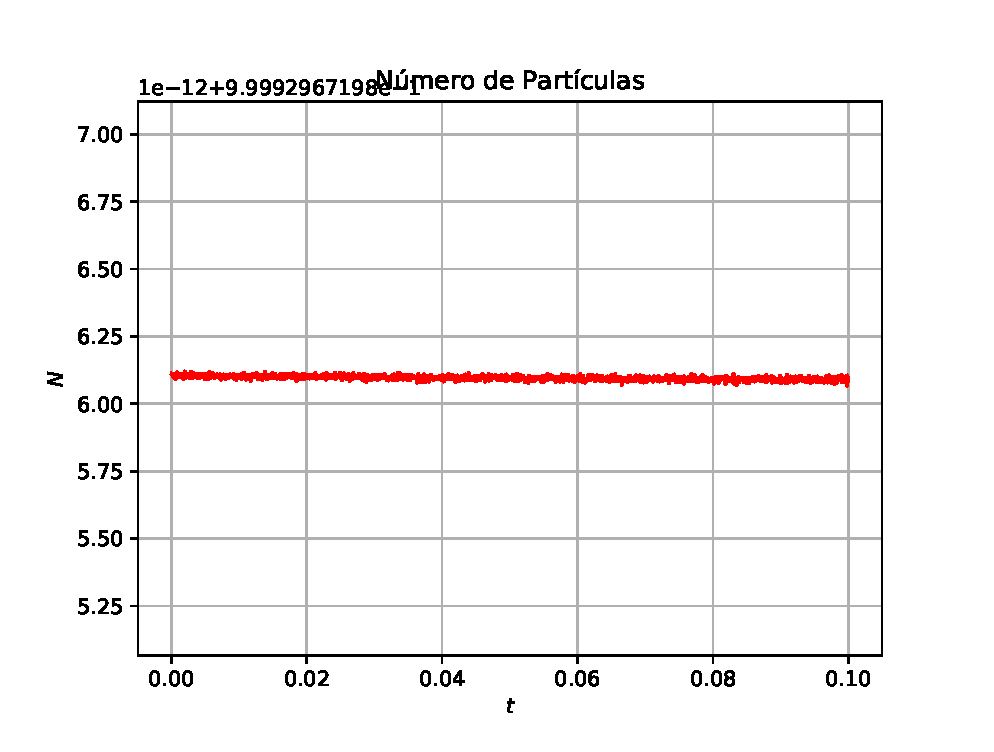
\includegraphics[scale=.4]{numpartupwind1}}
	\end{minipage}\par\smallskip
	\centering
	\subfloat[]{\label{faseupwind1}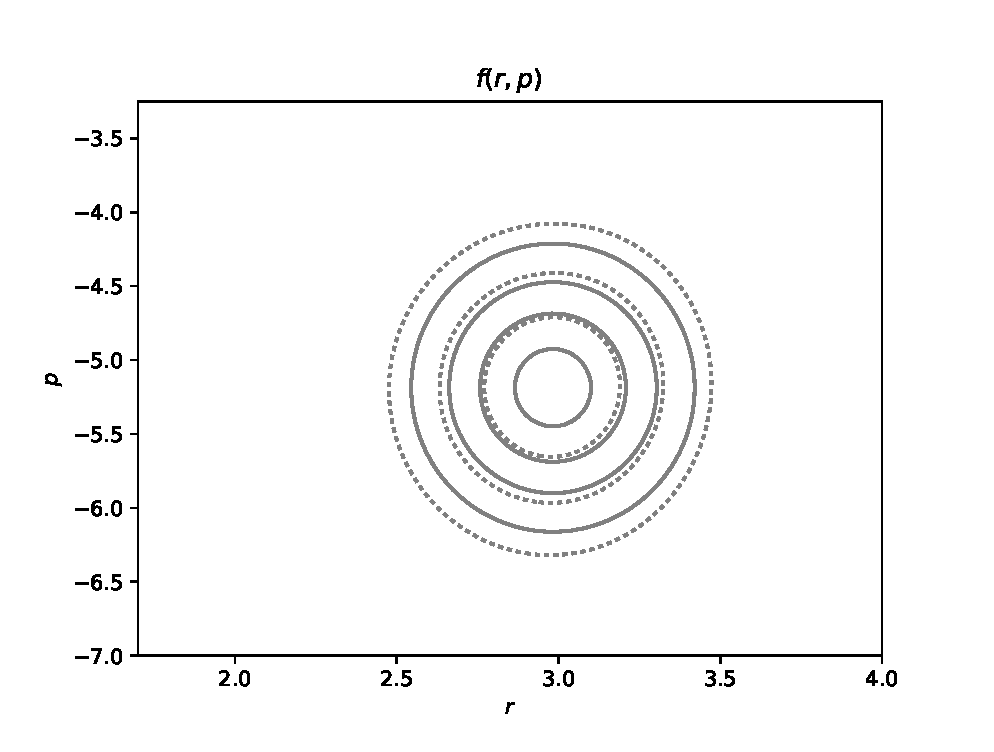
\includegraphics[scale=.6]{circupwind1}}
	\caption{Upwind de  primer orden. En a) se muestra el perfil de densidad, con el eje $x$ reescalado de manera que se pueda ver la variación entre la solución analítica (en rojo) y la solución numérica (en azul) considerando que el perfil debería mantenerse igual a la condición inicial ya que la ecuación de advección no cambia la forma de la función, en b) se muestra el número de partículas, que debe mantenerse constante para que el método sea útil para el presente estudio, y en c) se muestra $f$ en curvas de nivel, de manera que se pueda ver cómo cambia la forma de la función inicial en el espacio-fase al evolucionar, la solución analítica es la línea continua mientras que la numérica es la línea punteada.} 
	\label{upwind1}
\end{figure}
\begin{figure}[p]
	\begin{minipage}{.5\linewidth}
		\centering
		\subfloat[]{\label{densidadupwind2}\includegraphics[scale=.5]{densityupwind2}}
	\end{minipage}%
	\begin{minipage}{.5\linewidth}
		\centering
		\subfloat[]{\label{numpartupwind2}\includegraphics[scale=.4]{numpartmc}}
	\end{minipage}\par\smallskip
	\centering
	\subfloat[]{\label{faseupwind2}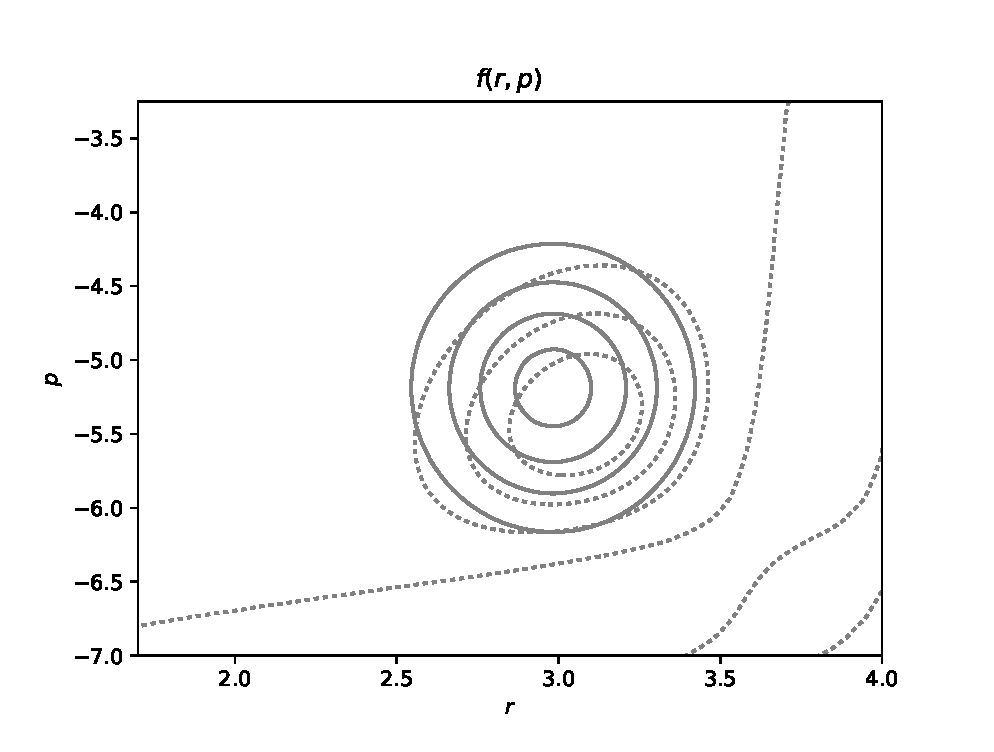
\includegraphics[scale=.6]{circupwind2}}
	\caption{Upwind de segundo orden. En a) se muestra el perfil de densidad, con el eje $x$ reescalado de manera que se pueda ver la variación entre la solución analítica (en rojo) y la solución numérica (en azul) considerando que el perfil debería mantenerse igual a la condición inicial ya que la ecuación de advección no cambia la forma de la función, en b) se muestra el número de partículas, que debe mantenerse constante para que el método sea útil para el presente estudio, y en c) se muestra $f$ en curvas de nivel, de manera que se pueda ver cómo cambia la forma de la función inicial en el espacio-fase al evolucionar, la solución analítica es la línea continua mientras que la numérica es la línea punteada.}
	\label{upwind2}
\end{figure}
\begin{figure}[p]
	\begin{minipage}{.5\linewidth}
		\centering
		\subfloat[]{\label{densidadlw}\includegraphics[scale=.5]{densitylw}}
	\end{minipage}%
	\begin{minipage}{.5\linewidth}
		\centering
		\subfloat[]{\label{numpartlw}\includegraphics[scale=.4]{numpartlw}}
	\end{minipage}\par\smallskip
	\centering
	\subfloat[]{\label{faselw}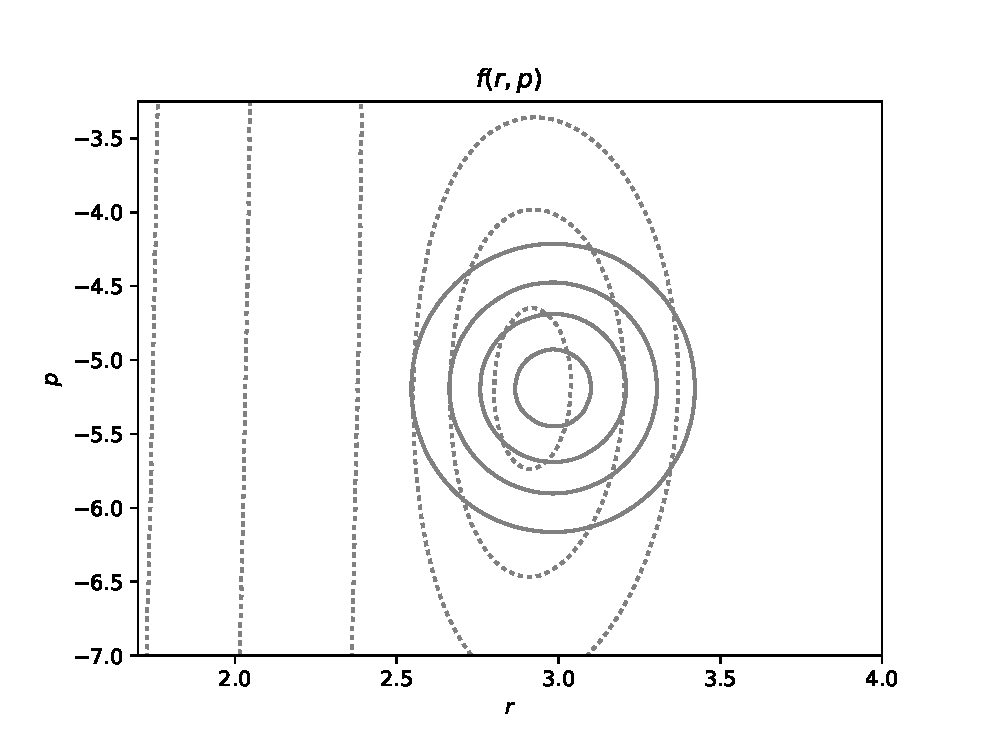
\includegraphics[scale=.6]{circlw}}
	\caption{Lax-Wendroff. En a) se muestra el perfil de densidad, con el eje $x$ reescalado de manera que se pueda ver la variación entre la solución analítica (en rojo) y la solución numérica (en azul) considerando que el perfil debería mantenerse igual a la condición inicial ya que la ecuación de advección no cambia la forma de la función, en b) se muestra el número de partículas, que debe mantenerse constante para que el método sea útil para el presente estudio, y en c) se muestra $f$ en curvas de nivel, de manera que se pueda ver cómo cambia la forma de la función inicial en el espacio-fase al evolucionar, la solución analítica es la línea continua mientras que la numérica es la línea punteada.}
	\label{lw}
\end{figure}
\begin{figure}[p]
	\begin{minipage}{.5\linewidth}
		\centering
		\subfloat[]{\label{densidadminmod}\includegraphics[scale=.5]{densityminmod}}
	\end{minipage}%
	\begin{minipage}{.5\linewidth}
		\centering
		\subfloat[]{\label{numpartminmod}\includegraphics[scale=.4]{numpartminmod}}
	\end{minipage}\par\smallskip
	\centering
	\subfloat[]{\label{faseminmod}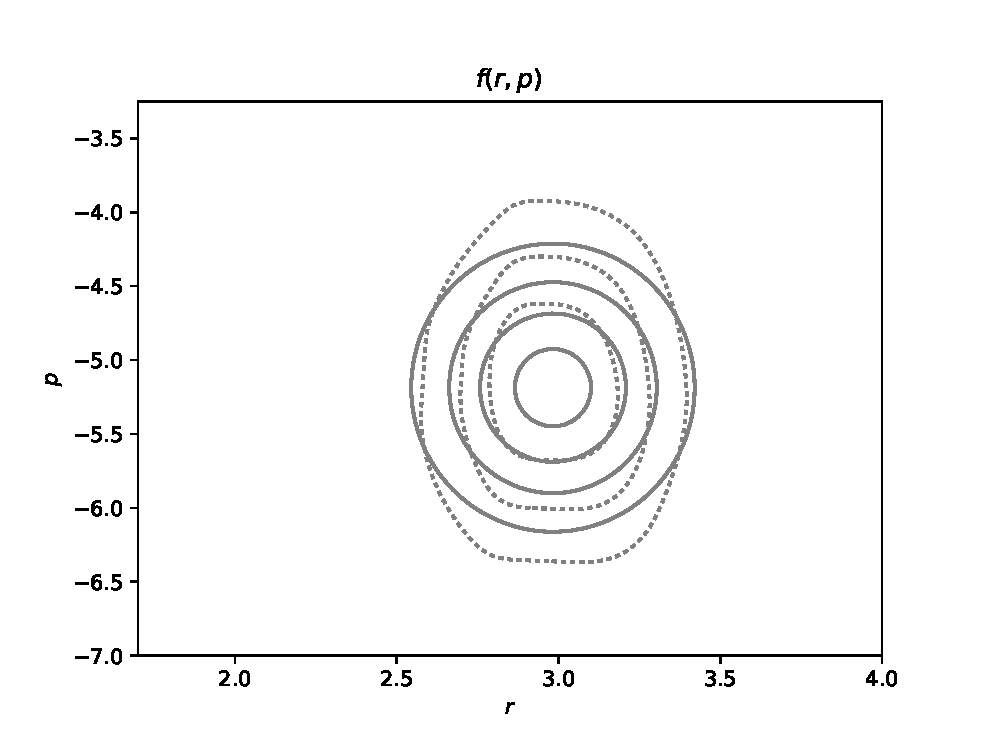
\includegraphics[scale=.6]{circminmod}}
	\caption{Limitador Minmod. En a) se muestra el perfil de densidad, con el eje $x$ reescalado de manera que se pueda ver la variación entre la solución analítica (en rojo) y la solución numérica (en azul) considerando que el perfil debería mantenerse igual a la condición inicial ya que la ecuación de advección no cambia la forma de la función, en b) se muestra el número de partículas, que debe mantenerse constante para que el método sea útil para el presente estudio, y en c) se muestra $f$ en curvas de nivel, de manera que se pueda ver cómo cambia la forma de la función inicial en el espacio-fase al evolucionar, la solución analítica es la línea continua mientras que la numérica es la línea punteada.}
	\label{minmod}
\end{figure}
\begin{figure}[p]
	\begin{minipage}{.5\linewidth}
		\centering
		\subfloat[]{\label{densidadsuperbee}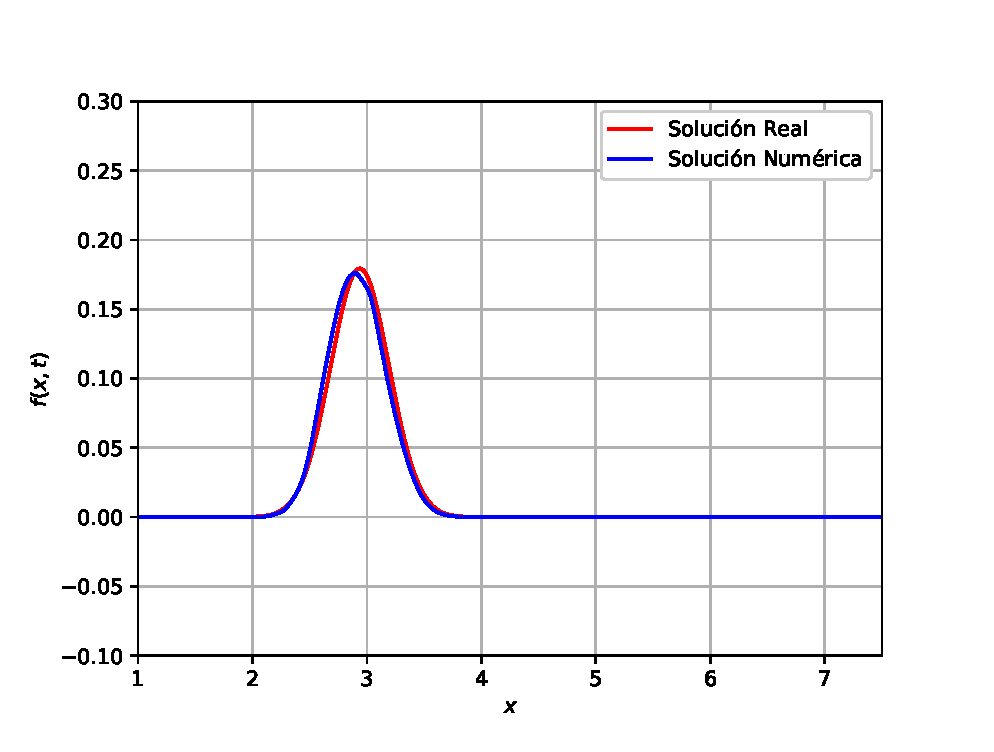
\includegraphics[scale=.5]{densitysuperbee}}
	\end{minipage}%
	\begin{minipage}{.5\linewidth}
		\centering
		\subfloat[]{\label{numpartsuperbee}\includegraphics[scale=.4]{numpartsuperbee}}
	\end{minipage}\par\smallskip
	\centering
	\subfloat[]{\label{fasesuperbee}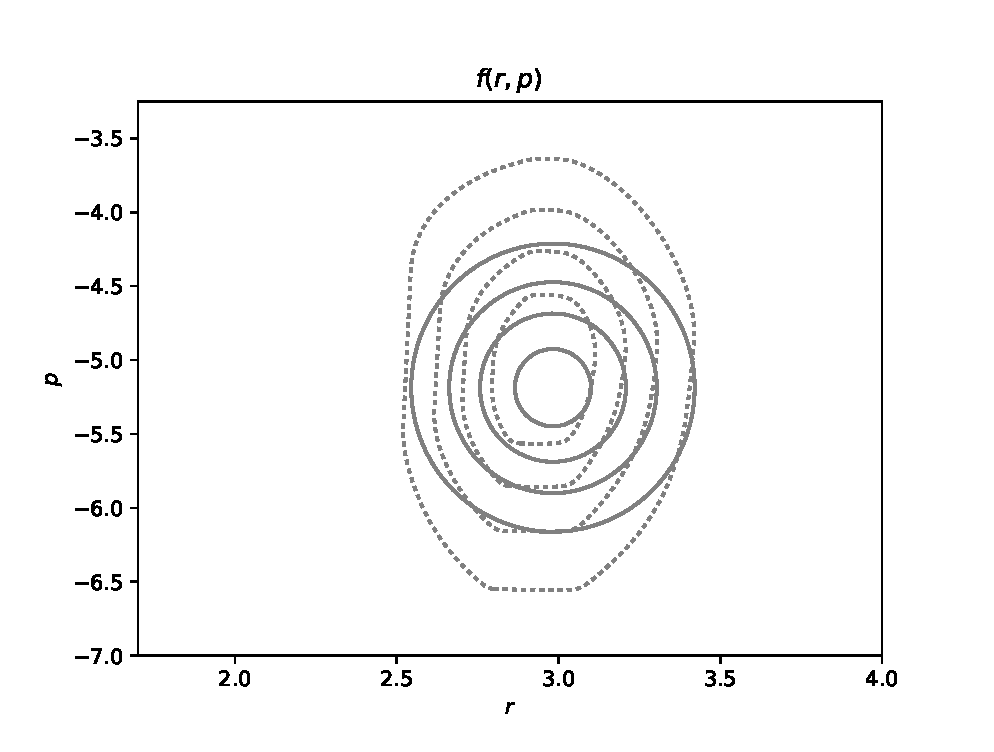
\includegraphics[scale=.6]{circsuperbee}}
	\caption{Limitador Superbee. En a) se muestra el perfil de densidad, con el eje $x$ reescalado de manera que se pueda ver la variación entre la solución analítica (en rojo) y la solución numérica (en azul) considerando que el perfil debería mantenerse igual a la condición inicial ya que la ecuación de advección no cambia la forma de la función, en b) se muestra el número de partículas, que debe mantenerse constante para que el método sea útil para el presente estudio, y en c) se muestra $f$ en curvas de nivel, de manera que se pueda ver cómo cambia la forma de la función inicial en el espacio-fase al evolucionar, la solución analítica es la línea continua mientras que la numérica es la línea punteada.}
	\label{superbee}
\end{figure}
\begin{figure}[p]
	\begin{minipage}{.5\linewidth}
		\centering
		\subfloat[]{\label{densidadmc}\includegraphics[scale=.5]{densitymc}}
	\end{minipage}%
	\begin{minipage}{.5\linewidth}
		\centering
		\subfloat[]{\label{numpartmc}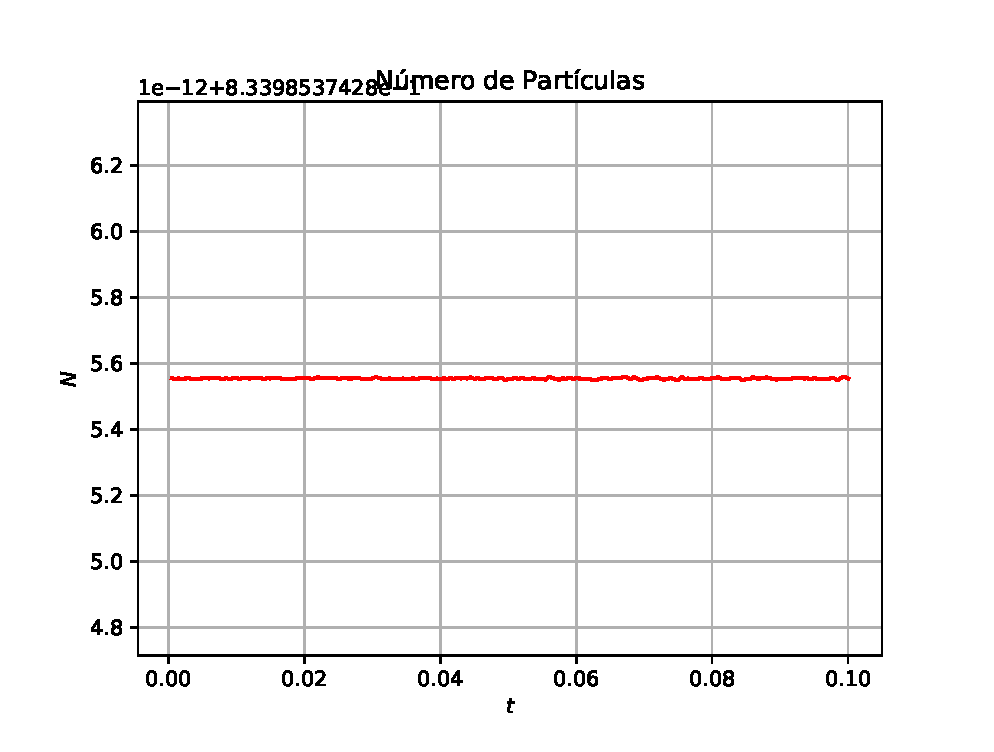
\includegraphics[scale=.4]{numpartupwind2}}
	\end{minipage}\par\smallskip
	\centering
	\subfloat[]{\label{fasemc}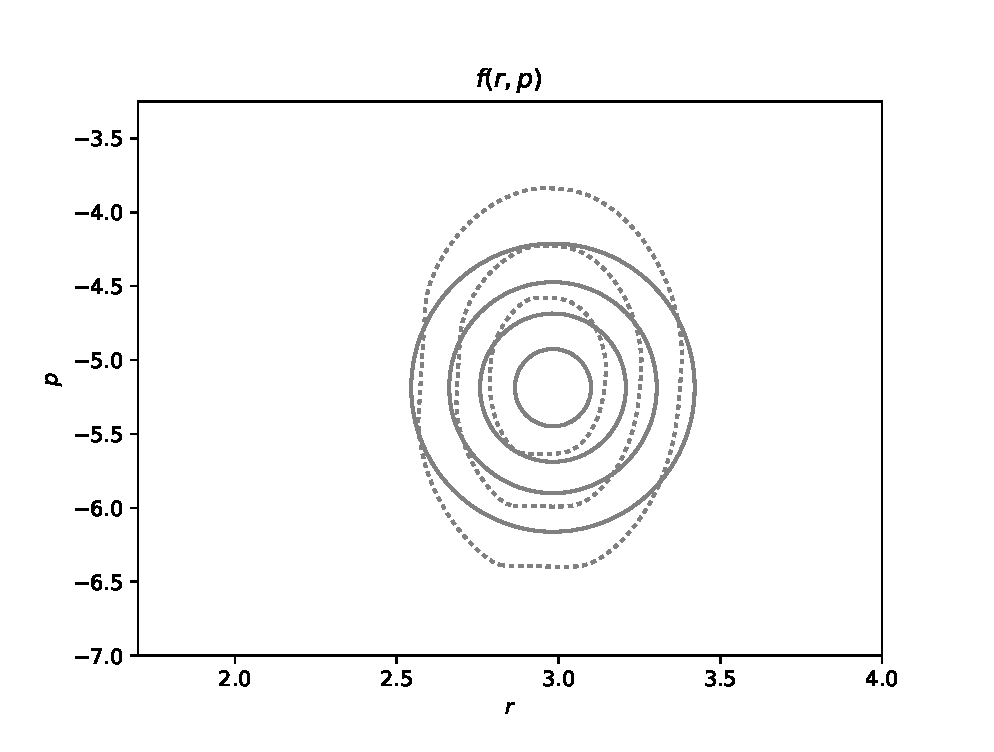
\includegraphics[scale=.6]{circmc}}
	\caption{Limitador Monotonized Central. En a) se muestra el perfil de densidad, con el eje $x$ reescalado de manera que se pueda ver la variación entre la solución analítica (en rojo) y la solución numérica (en azul) considerando que el perfil debería mantenerse igual a la condición inicial ya que la ecuación de advección no cambia la forma de la función, en b) se muestra el número de partículas, que debe mantenerse constante para que el método sea útil para el presente estudio, y en c) se muestra $f$ en curvas de nivel, de manera que se pueda ver cómo cambia la forma de la función inicial en el espacio-fase al evolucionar, la solución analítica es la línea continua mientras que la numérica es la línea punteada.}
	\label{mc}
\end{figure}
\newpage

Se observa que, de acuerdo con la teoría, los métodos a primer orden generan efectos disipativos en la función de distribución, como se puede ver en la figura \ref{upwind1}, mientras que aquellos que son a segundo orden tienden a introducir oscilaciones espurias, como se puede ver en las figuras \ref{upwind2} y \ref{lw}. Además, ninguno de estos preserva bien la forma de la función de distribución vista desde el espacio-fase, aún cuando pareciera que el perfil de densidad no cambia drásticamente. En el caso de los limitadores, debido a la dependencia  en las coordenadas que tienen los campos de velocidades, el perfil de densidad no se preserva exactamente pero sí es una buena aproximación, siendo que además, vista desde el espacio-fase, la forma de la función de distribución no presenta cambios tan alejados a la solución analítica como en el caso de los métodos a primer y segundo orden.

A partir del análisis anterior, se concluye que de las tres opciones de limitadores $\Psi$ que se estudiaron, el conocido como ``Monotonized Central'' preserva moderadamente bien tanto el perfil de densidad de la función de distribución, como también su forma general vista en el espacio-fase. Preserva también el número de partículas, por lo que es este limitador el que se utiliza para el estudio numérico\footnote{Este es el limitador que se utilizó en un estudio previo en el que se trata meramente el caso Newtoniano de la ecuación de Vlasov, estudio que puede consultarse en \citet{Jimenez2016}.}.

\section{Integración Numérica: Regla de Simpson Compuesta}
\noindent
Para obtener las cantidades físicas del sistema que se está estudiando, se deben de obtener un conjunto de cuadraturas que dependen de la función de distribución en una y dos dimensiones.  Para esto, se utiliza la regla de Simpson compuesta\footnote{Ver \citet{mayers}.}, que consiste en aproximar cada subintervalo de la función a integrar $f(x)$ mediante polinomios de segundo grado. 

\subsection{Una dimensión}
\noindent

Básicamente, la integral en una sola dimensión de una cierta función $f(x)$ se aproxima como
\begin{equation}
\int_{a}^{b}f\left(x\right)\ \text{d}x\approx\frac{h}{3}\left[f\left(x_0\right)+2\sum_{j=1}^{n/2-1}f(x_{2j})+4\sum_{j=1}^{n/2}f(x_{2j-1})+f(x_n)\right]+\mathcal{O}\{h^4\}
\end{equation}
donde el intervalo de integración $[a,b]$ se divide en $n$ subintervalos (siendo $n$ un número par) $\left[x_{i-1},x_i\right]_{i=1}^{2m}$ de ancho $h=\frac{b-a}{n}$, donde $x_i=a+ih$. 

\subsection{Dos dimensiones}
\noindent
Para una integración numérica en dos dimensiones, basta con hacer una generalización de la regla de Simpson compuesta dada en la sección anterior. Se considera una función $f(x,y)$ sobre un rectángulo $\mathbf{R}=\{(x,y):a\leq x\leq b, c\leq y\leq d\}$. El intervalo $[a,b]$ esta dividido en $2m$ subintervalos $\left[x_{i-1},x_i\right]_{i=1}^{2m}$ de ancho $h=\frac{b-a}{2m}$, donde $x_i=x_0+ih$. Análogamente, el intervalo $[c,d]$ se divide en $2n$ subintervalos $\left[y_{j-1},y_j\right]_{j=1}^{2n}$ de ancho $k=\frac{d-c}{2n}$, donde $y_j=y_0+jk$. La integral en dos dimensiones se aproxima como
\begin{align*}
\int_a^b \int_c^d f(x,y)\ \text{d}x\ \text{d}y&\approx \frac{1}{9}hk\Bigg[f(a,c)+f(a,d)+f(b,c)+f(b,d)\bigg.\\
&+4\sum_{j=1}^n f(a,y_{j-1})+2\sum_{j=1}^{n-1}f(a,y_j)+4\sum_{j=1}^{n}f(b,y_{j-1})+2\sum_{j=1}^{n-1}f(b,y_j)\\
&+4\sum_{i=1}^m f(x_{i-1},c)+2\sum_{i=1}^{m-1}f(x_i,c)+4\sum_{i=1}^{m}f(x_{i-1},d)+2\sum_{i=1}^{m-1}f(x_i,d)\\
&+16\sum_{j=1}^{n}\bigg(\sum_{i=1}^{m}f(x_{i-1},y_{j-1})\bigg)+8\sum_{j=1}^{n-1}\bigg(\sum_{i=1}^m f(x_{i-1},y_j)\bigg)\\
&+8\sum_{j=1}^n\bigg(\sum_{i=1}^{m-1}f(x_i,y_{j-1})\bigg)+4\sum_{j=1}^{n-1}\bigg(\sum_{i=1}^{m-1}f(x_i,y_j)\bigg))\Bigg]+\mathcal{O}(h^4)+\mathcal{O}(k^4)
\end{align*}

\chapter{Simulaciones Numéricas de la ecuación de Vlasov en la solución de Schwarzshild}
\noindent
En este capítulo se escriben explícitamente las ecuaciones a resolver numéricamente. Comparando la ecuación \eqref{conserv2D} con \eqref{sisvlasov1}, se puede ver que la ecuación de Vlasov esta escrita como una ley de conservación, donde las cantidades conservadas son
\begin{align}
\mathcal{F}_x=&f_*\frac{\text{d}x^i}{\text{d}t}\\
\mathcal{F}_p=&f_*\frac{\text{d}p_i}{\text{d}t}
\end{align}
siendo estos los \textit{flujos} en la dirección $x^i$ y $p_i$, respectivamente. De esta manera, es posible utilizar los métodos limitadores de flujo vistos en el capítulo \ref{metnum} para encontrar la evolución de la función de distribución bajo una cierta métrica de fondo, en este caso, se utilizará la métrica de Schwarzschild en coordenadas usuales así como también en coordenadas de Kerr-Schild. 

En el trabajo original de Schwarzschild, la coordenada radial posee una singularidad física en el origen y una singularidad debida a las coordenadas utilizadas en el horizonte de eventos, por lo tanto, en realidad no se estudia al agujero negro, solamente la vecindad de dicho horizonte. Con el objetivo principal de entender la singularidad en las coordenadas que se da en el horizonte de eventos, la métrica de Schwarzschild se ha escrito en otros sistemas de coordenadas que a distancias radiales grandes son iguales. Uno de estos sistemas de coordenadas es el de Kerr-Schild, cuyos términos de la métrica no se indeterminan en el horizonte.

\newpage
\section{Estudio numérico y descripción del código}
\noindent
Como ya se ha mencionado, se utilizó el haz cotangente como espacio fase, por lo que el estudio se realizará en una malla con espaciamiento constante $\text{d}r$ en el eje $r$ y $\text{d}p$ en el eje $p$, cuyo dominio estará dado por $\left\{\left.\left(r,p_r\right)\right|r_{\text{min}}\leq r\leq r_{max},\ p_{\text{min}}\leq p\leq p_{\text{max}}\right\}$, de manera que existen $N_r$ puntos de la malla en $r$ y $N_p$ en $p$, dados por
\begin{equation}
\nonumber
N_r=\text{int}\left(\frac{r_{\text{max}}-r_{\text{min}}}{\text{d}r}\right)\hspace{1cm}N_p=\text{int}\left(\frac{p_{\text{max}}-p_{\text{min}}}{\text{d}p}\right)
\end{equation}

Se utilizaron condiciones de frontera radiativas para la evolución numérica, escritas de la siguiente forma
\begin{eqnarray*}
\partial_t f+\upsilon_x\partial_x f=0&\hspace{1cm}& \text{Frontera $x=x_{\text{max}}$ con }\upsilon_x>0\\
f=0&\hspace{1cm}& \text{Frontera $x=x_{\text{min}}$ con }\upsilon_x>0\\
f=0&\hspace{1cm}& \text{Frontera $x=x_{\text{max}}$ con }\upsilon_x\leq 0\\
\partial_t f+\upsilon_x\partial_x f=0&\hspace{1cm}& \text{Frontera $x=x_{\text{min}}$ con }\upsilon_x\leq 0
\end{eqnarray*}
Estas condiciones se implementan tanto para la malla en $r$ como para la malla en $p$ (substituyendo $x=r$ y $x=p$ en las ecuaciones anteriores), y donde $\upsilon_x$ estaría dada, en el primer caso, por $\upsilon_r=\text{d}r/\text{d}t$, y en el segundo caso, por $\text{d}p/\text{d}t$. Físicamente, estas condiciones quieren decir que las partículas representadas por la función de distribución pueden dejar el dominio numérico si así lo describe su dinámica (procurando una mínima reflexión), más no es posible que se introduzca nueva información desde el exterior del dominio.

En las coordenadas de Schwarzschild, dada la singularidad (debida a las coordenadas) de los componentes de la métrica en el horizonte de eventos $r=2M$, se tomó $r_{\text{min}}=2M+\text{d}r/2$. Esto habla de que no es posible estudiar la dinámica más allá del horizonte de eventos. Para las coordenadas de Kerr-Schild, al remover dicha singularidad con un cambio de coordenadas, queda solo aquella en $r=0$, por lo que, para evitarla, y dado que principalmente se busca estudiar los efectos físicos fuera del agujero negro, se realiza una ``excisión'' de este último\footnote{Ver \citet{alcubierre}, sección 6.5.}, que en este caso no fue más que remover dicha singularidad del dominio computacional, dado que el interior del agujero negro no debería afectar el exterior. Para lograr esto, simplemente se tomó $r_{\text{min}}=M/4$. El código se realizó en el lenguaje de programación Fortran 90 GNU.

%\lstinputlisting[language=Fortran, firstline=224, lastline=298]{VlasovSchSphere.f90} 

%\lstinputlisting[language=Fortran, firstline=1128, lastline=1169]{VlasovSchSphere.f90} 

\subsection{Función de distribución}
\noindent
Para evolucionar el código se utilizó una suma de funciones de distribución gaussianas como dato inicial, la cual tiene la siguiente forma
\begin{align}
\nonumber
f(t=0,r,p_r,L)&=K\left(\exp\left[-\frac{\left(r-r_c\right)^2}{\sigma_r^2}-\frac{\left(p-p_{rc}\right)^2}{\sigma_{p_r}^2}\right]\right.\\
&\left.+\exp\left[-\frac{\left(r+r_c\right)^2}{\sigma_r^2}-\frac{\left(p+p_{rc}\right)^2}{\sigma_{p_r}^2}\right]\right)\delta(L-L_c)
\label{gaussian}
\end{align}
donde $K=\frac{N_0}{\pi\sigma_r\sigma_p}$, con $N_0$ el número de partículas, $\sigma_r$ y $\sigma_p$ son cantidades arbitrarias que determinan la anchura de las funciones, y $r_c$, $p_{rc}$ y $L_c$ determinan dónde estarán centradas. Se tomó la suma de dos gaussianas con el objetivo de que la integral pueda realizarse analíticamente para obtener que es igual a $N_0$, el número de partículas iniciales. Escoger esta condición también es necesario en el caso Newtoniano para que se cumpla la condición de frontera $f(-r,-p)=f(r,p)$, por lo que se toma de la misma forma en este trabajo para una mejor comparación, entendiéndose que esto no influye el resultado del estudio ya que las gaussianas no se afectan mutuamente en este caso (ya que la métrica es estática, sin embargo, esto deberá influir en el caso en que no lo sea).

Además de lo anterior, se escogió esta forma para la función de distribución debido a su sencillez, y únicamente para probar que lo obtenido con el método numérico implementado en este estudio sea coherente con la teoría y con resultados previos, sin embargo, existen otros tipos de función de distribución que se utilizan para modelar otros objetos, por ejemplo, cúmulos de estrellas relativistas en equilibrio, representados por la función de distribución de Maxwell-Boltzmann\footnote{Ver \citet{Shapiro2010}, sección 8.2.}. 

Usando la función de distribución dada por \eqref{gaussian}, se observa que las ecuaciones \eqref{K} y \eqref{rF} toman la forma\footnote{En este apartado se utiliza la propiedad
	\begin{equation*}
	\int_{-\infty}^{\infty} g(u)\ \delta(u-u_0)\ \text{d}u=g(u_0)
	\end{equation*}} 
\begin{align}
\left<K_{\text{tot}}\right>&=\frac{4\pi^2}{m}\int L_c\left(p_r^2+\frac{L_c^2}{r^2}\right)f\ \text{d}r\ \text{d}p_r\\
\left<rF\right>&=-8\pi^2\int L_cr\ \partial_r\Phi\ f\ \text{d}r\ \text{d}p_r\
\end{align}
donde ahora
\begin{align}
\nonumber
f(t=0,r,p_r)=&\frac{N_0}{\pi\sigma_r\sigma_p}\left(\exp\left[-\frac{\left(r-r_c\right)^2}{\sigma_r^2}-\frac{\left(p-p_{rc}\right)^2}{\sigma_{p_r}^2}\right]\right.\\
&\left.+\exp\left[-\frac{\left(r+r_c\right)^2}{\sigma_r^2}-\frac{\left(p+p_{rc}\right)^2}{\sigma_{p_r}^2}\right]\right)
\end{align}

\section{Coordenadas de Schwarzschild}
\noindent
Es común utilizar coordenadas esféricas polares estándar $(t,r,\theta,\phi)$ para escribir la métrica de Schwarzschild\footnote{A estas se les conoce como coordenadas \textit{de Schwarzschild} o \textit{usuales}.}. El elemento de línea para esta métrica en coordenadas usuales es 
\begin{equation}
\text{d}S^2=-\left(1-\frac{2M}{r}\right)\ \text{d}t^2 +\left(1-\frac{2M}{r}\right)^{-1}\ \text{d}r^2 +r^2\left(\text{d}\theta^2+\sin^2\theta\ \text{d}\phi^2\right)
\end{equation}
donde se tiene que $t$ es la coordenada temporal, $r$, $\theta$ y $\phi$ son las coordenadas esféricas y $M$ es la masa característica de la geometría de Schwarzschild. En estas coordenadas, las cantidades 3+1 son:
\begin{equation}
\alpha=\left(1-\frac{2M}{r}\right)^{\frac{1}{2}}, \hspace{1cm}A=\left(1-\frac{2M}{r}\right)^{-1}, \hspace{1cm}\beta_r=\beta^r=0, \hspace{1cm}B=\psi=1
\end{equation}
las cuales en general, dependen del tiempo, aunque en este caso se estudia únicamente una métrica de fondo que no evoluciona en el tiempo.

Dado que la métrica de Schwarzschild es independiente de $t$ y $\phi$, deben existir vectores de Killing $\kappa^\mu$ en estas direcciones tales que sea posible encontrar cantidades conservadas. Definiendo $p^\mu=\text{d}x^\mu/\text{d}\lambda$ (con $\lambda=\tau/m$, siendo $m$ la masa en reposo de una partícula) un vector tangente al camino $x^\mu\left(\tau\right)$ de una partícula en el espacio tiempo, se puede demostrar que $\kappa^\mu p_\mu$ es una cantidad conservada\footnote{Ver \citet{Raine2014}, capítulo 2.}. Considerando la dirección temporal dada por $\kappa^\mu=\left(1,0,0,0\right)$, se tiene
\begin{align}
g_{\mu\nu}\kappa^\mu p^\nu=g_{tt}\kappa^tp^t=g_{tt}p^{t}=-E=\text{const}\\
\Rightarrow -\left(1-\frac{2M}{r}\right)\frac{\text{d}t}{\text{d}\lambda}=-E
\end{align}
se observa que $p_t=g_{t\nu}p^\nu=g_{tt}p^t$ y por lo tanto $p_t=-E$, siendo $E$ la energía de una partícula.

Análogamente, para la simetría en dirección de $\phi$, se tiene $\kappa=\left(0,0,0,1\right)$, y usando $p^\phi=\text{d}\phi/\text{d}\lambda$ se tiene
\begin{eqnarray}
g_{\mu\nu}\kappa^\mu p^\nu=g_{\phi\phi}\kappa^\phi p^\phi=g_{\phi\phi}p^\phi=L=\text{const}\\
\Rightarrow r^2\frac{\text{d}\phi}{\text{d}\lambda}=L
\end{eqnarray}
nuevamente, $p_\phi=g_{\phi\nu}p^\nu=g_{\phi\phi}p^\phi$, y por lo tanto $p_\phi=L$, siendo $L$ el momento angular de una partícula relativo a un observador en el infinito.

Dado que el campo gravitacional es esféricamente simétrico, cualquier órbita de un objeto en caída libre debe mantenerse en un plano, por lo que se toma $\theta=\pi/2$ de manera que $\sin\theta=1$.

Usando la condición de normalización $g^{\mu\nu}p_\mu p_\nu=-m^2$, y substituyendo los coeficientes métricos y las cantidades conservadas $p_t$ y $p_\phi$, se obtiene
\begin{equation}
-\left(1-\frac{2M}{r}\right)^{-1}E^2+\left(1-\frac{2M}{r}\right)p_1^2+\frac{L^2}{r^2}=-m^2
\end{equation}
Dado que $p_1=g_{11}p^1=\left(1-2M/r\right)^{-1}\left(\text{d}r/\text{d}\lambda\right)$, entonces\footnote{En este punto se utiliza la notación $\tilde{E}=E/m$ y $\tilde{L}=L/m$ para simplificar las expresiones.}
\begin{equation}
\left(\frac{\text{d}r}{\text{d}\tau}\right)^2=\tilde{E}-\left(1+\frac{\tilde{L}^2}{r^2}\right)\left(1-\frac{2M}{r}\right)=\tilde{E}^2-V^2
\label{difenergias}
\end{equation}
Se deduce que el potencial efectivo $V$ en Schwarzschild\footnote{Ver \citet{schutz}, p. 284.} tiene la siguiente forma 
\begin{equation}
V^2(r)=\left(1-\frac{2M}{r}\right)\left(1+\frac{\tilde{L}^2}{r^2}\right)
\end{equation}
para el radio donde se dan órbitas circulares $r_c$, debe suceder que $\left.\frac{\text{d}r}{\text{d}\tau}\right|_{r_c}=0$ y $\left.\frac{\text{d}^2r}{\text{d}\tau^2}\right|_{r_c}=0$. La primera de estas condiciones implica $\tilde{E}^2=V^2$, por lo que la energía debe de situarse en la curva del potencial efectivo. La segunda implica $\left.\frac{dV^2}{dr}\right|_{r_c}=0$, por lo tanto
\begin{equation*}
\frac{\text{d}V^2}{\text{d}r}=\frac{2M}{r^2}\left(1+\frac{\tilde{L}^2}{r^2}\right)-\frac{2\tilde{L}^2}{r^3}\left(1-\frac{2M}{r}\right)\hspace{0.5cm} \Rightarrow\hspace{0.5cm} r_c^2-\frac{\tilde{L}^2r_c}{M}+3\tilde{L}^2=0
\end{equation*}
de donde se puede despejar $r_c$ en términos de $\tilde{L}$ (de manera que dado un momento angular, podemos encontrar un radio para una órbita circular), o al contrario, $\tilde{L}$ en términos de $r_c$ (para que, dada una $r_c$ en la cual se quiera una órbita circular, podamos encontrar $\tilde{L}$ que permita esa órbita). Análogamente, se puede obtener $\tilde{E}_c$ substituyendo $\tilde{L}_c$ en \eqref{difenergias}, con lo que se obtiene
\begin{align}
r_c(\tilde{L})&=\frac{\tilde{L}^2}{2M}\pm\frac{1}{2}\sqrt{\frac{\tilde{L}^4}{M^2}-12\tilde{L}^2}
\label{rc}\\
\tilde{L}_c(r)&=\sqrt{\frac{Mr}{1-\frac{3M}{r}}}
\label{Lc}\\
\tilde{E}_c(r)&=\left(1-\frac{2M}{r}\right)\sqrt{1-\frac{3M}{r}}
\label{Ec}
\end{align}
En \eqref{rc}, la raíz más pequeña es un máximo de $V$ y es inestable, la raíz más grande es estable mientras se cumpla $\tilde{L}\geq\sqrt{12}M$. Si $\tilde{L}\leq\sqrt{12}M$, se tiene que $r_c$ se vuelve un número complejo y por lo tanto no existe un radio para órbitas circulares. En la figura \ref{schpotential} se muestra la gráfica de este potencial para valores de $\tilde{L}$ mayor, menor e igual a $\sqrt{12}M$, y en la figura \ref{newtpot} se muestra la gráfica del potencial Newtoniano para valores arbitrarios de $L$. Se observa que para el potencial de Schwarzschild, la pared de potencial depende de $\tilde{L}$, y existen puntos mínimos y barrera de potencial únicamente para $\tilde{L}\geq\sqrt{12}M$, mientras que para el potencial Newtoniano la barrera de potencial siempre va a infinito y siempre existe un punto crítico mínimo. 

\begin{figure}[H]
	\begin{minipage}{.5\linewidth}
		\centering
		\subfloat[]{\label{schpotential}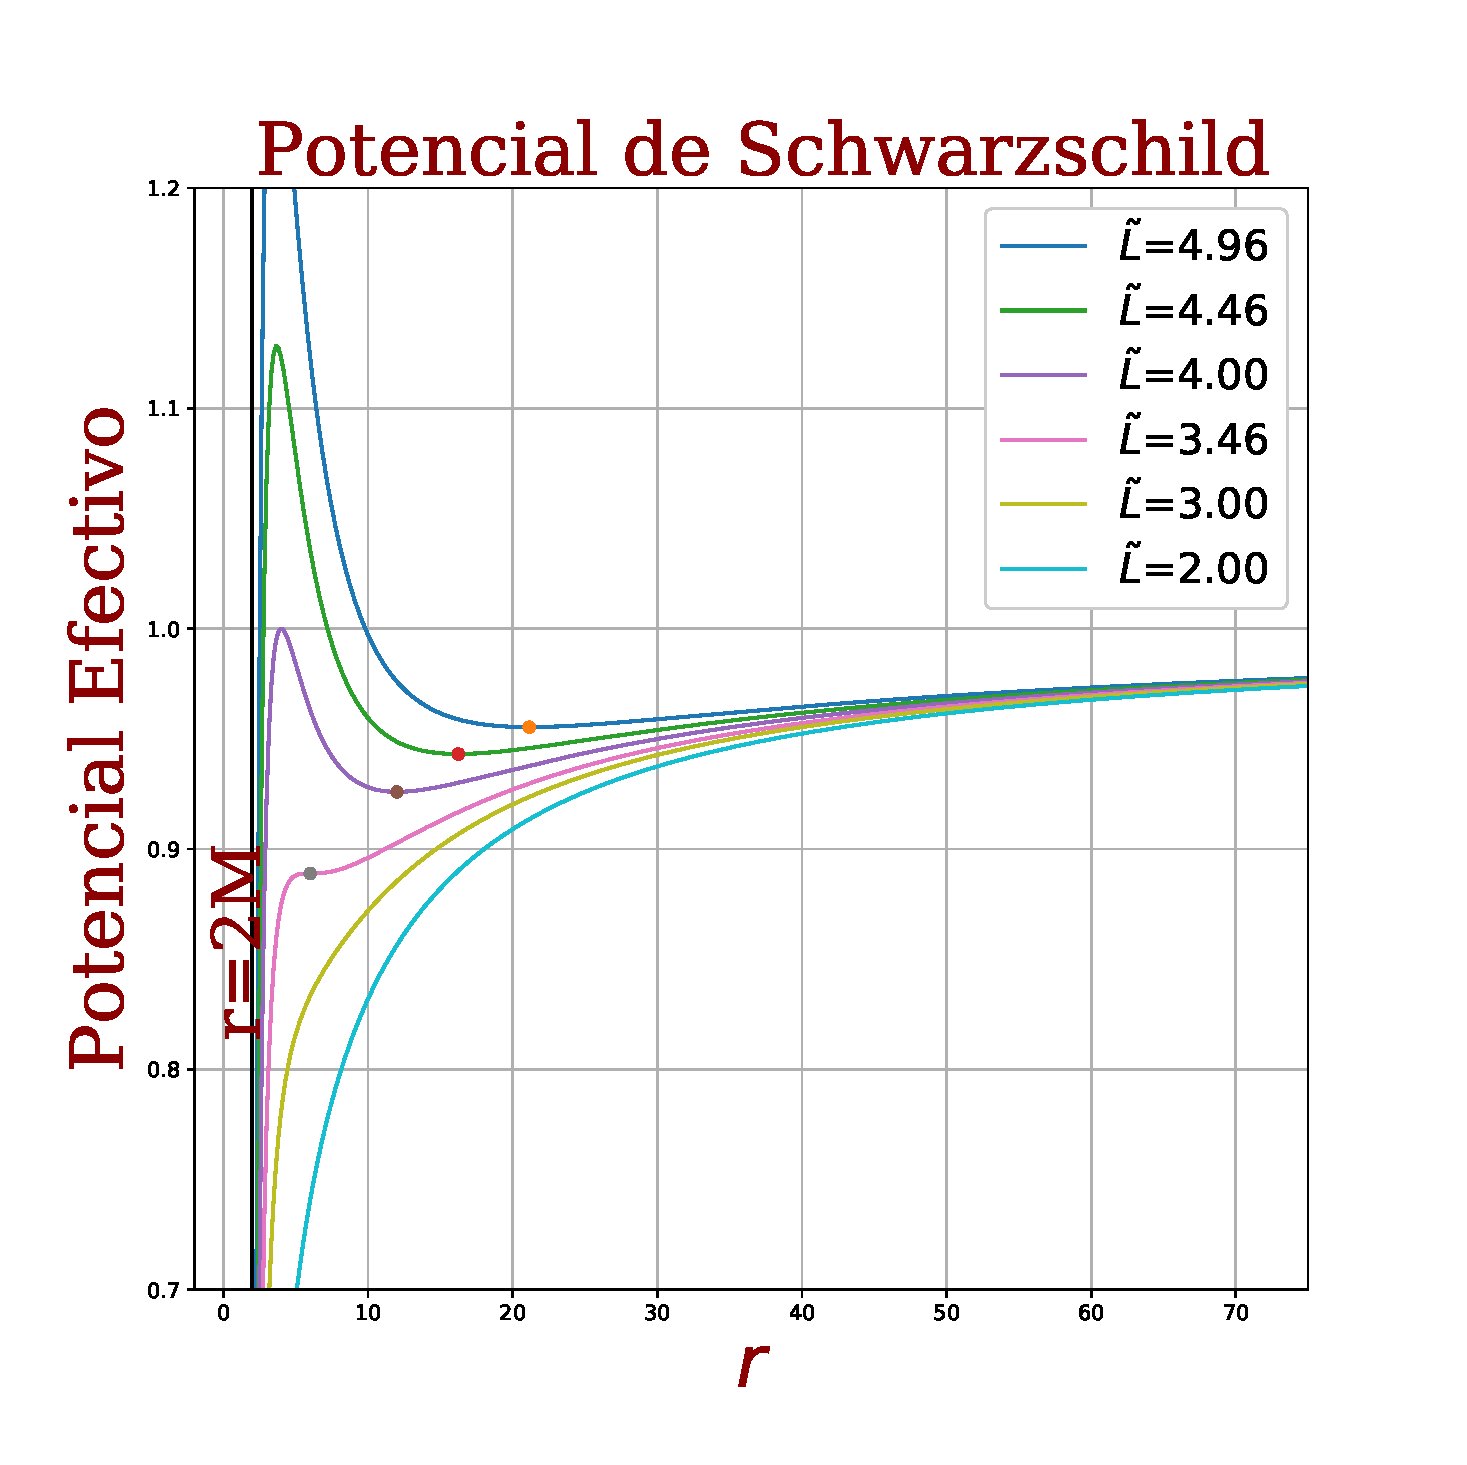
\includegraphics[scale=.34]{schpotential}}
	\end{minipage}%
	\begin{minipage}{.5\linewidth}
		\centering
		\subfloat[]{\label{newtpot}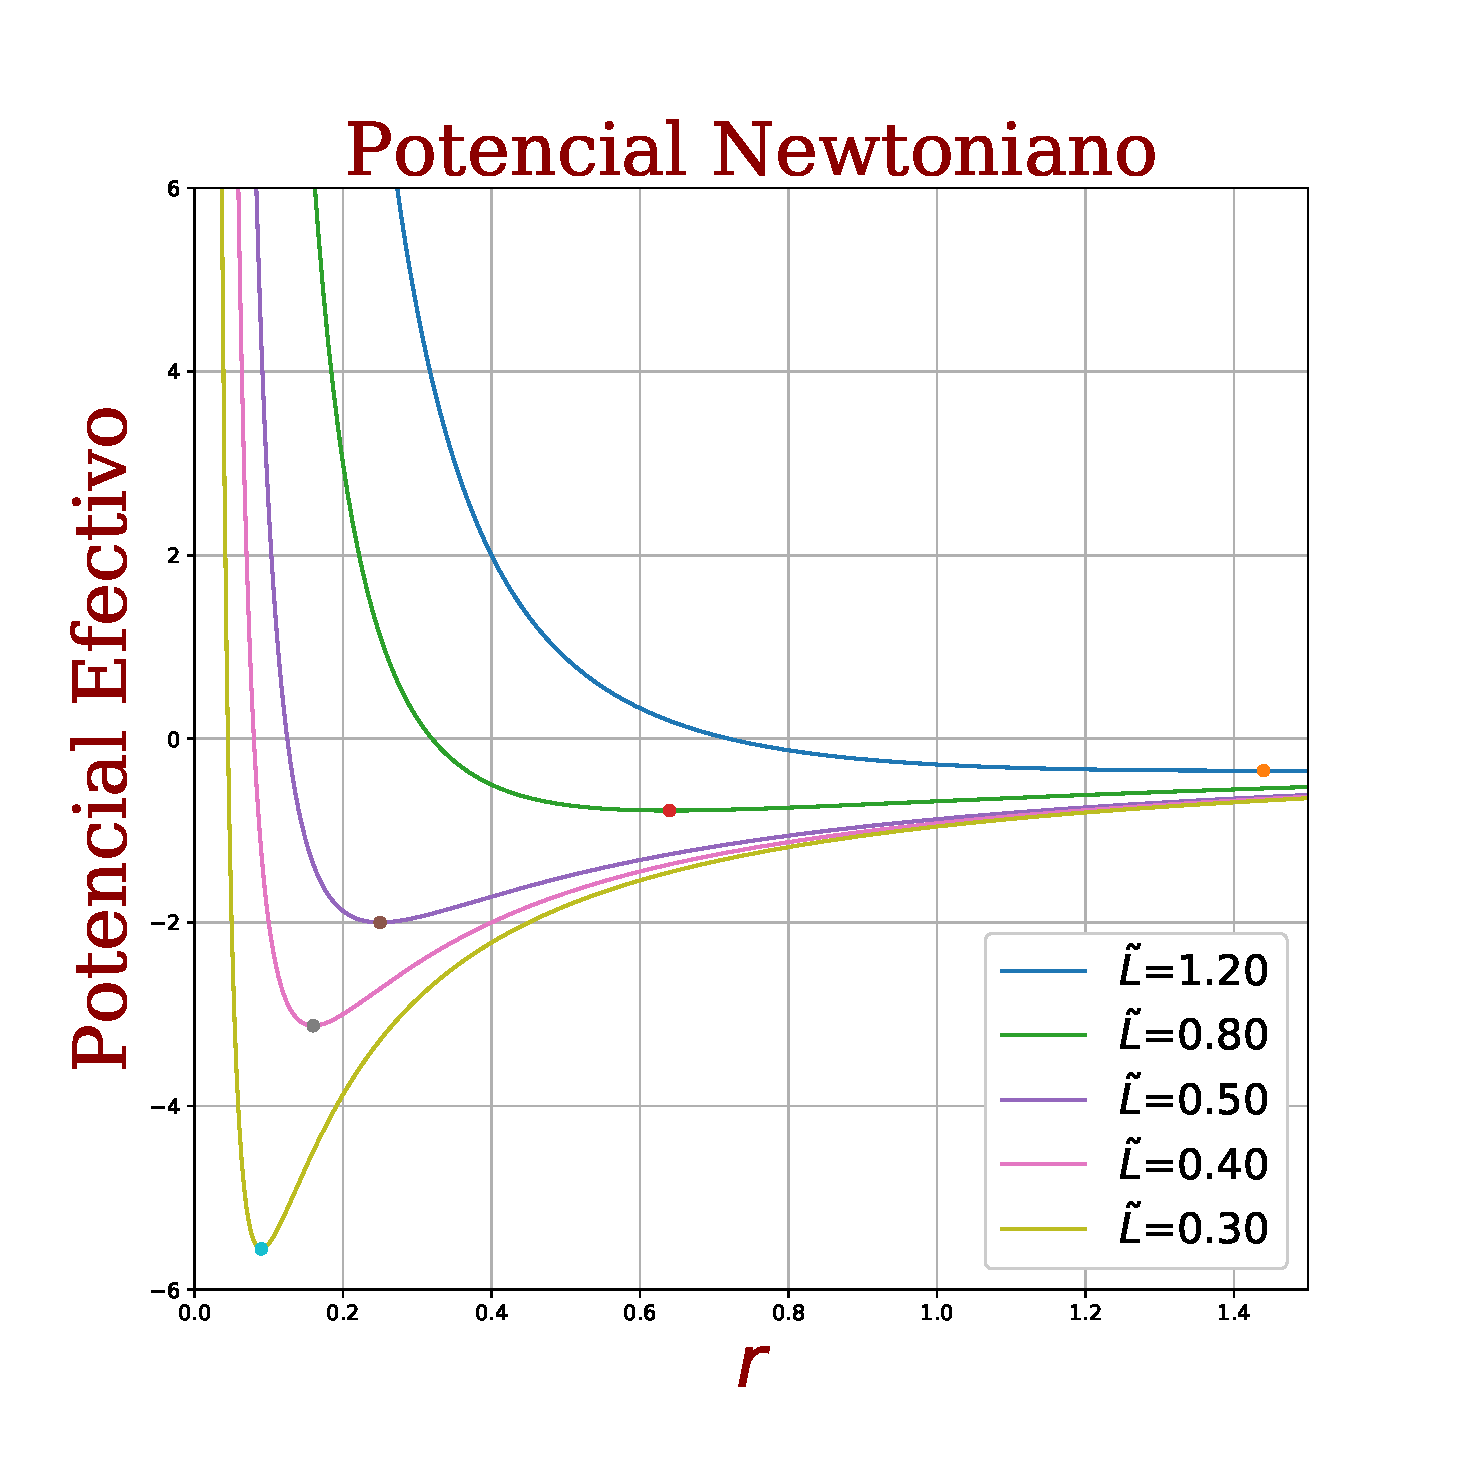
\includegraphics[scale=.34]{newtpot}}
	\end{minipage}
	\caption{Potencial de Schwarzschild y Newtoniano para valores distintos de $\tilde{L}$.}
\end{figure}

\subsection{Resultados numéricos}
\noindent
En la tabla \ref{datossch} se muestran las cantidades utilizadas para realizar las simulaciones en coordenadas de Schwarzschild. Para el análisis de convergencia se tomó un espaciamiento $\Delta t$ y se hicieron tres simulaciones, con $\Delta t$, $\Delta t/2$ y $\Delta t/4$. Los factores de Courant $\rho_r\ \text{d}r/\text{d}t$ y $\rho_p\ \text{d}p_r/\text{d}t$ siempre cumplen la condición \eqref{cfl}, lo cual se comprobó usando los máximos valores de $\text{d}r/\text{d}t$ y $\text{d}p_r/\text{d}t$ en toda la malla, sin embargo, sucede que aun cumpliendo con esta condición, algunos de los resultados para ciertos factores de Courant siguen siendo inestables. Esto último probablemente se deba a que la condición de estabilidad se deduce suponiendo que la velocidad en la ecuación de advección es constante, por lo que es de esperarse que no se cumpla la misma condición para velocidades dependientes (en este caso) de $r$ y $p$. 

Es importante destacar que, aún cuando físicamente no tiene sentido tomar $M=m=1\ \text{m}$, matemáticamente el valor de $M$ solamente afecta la ``escala'' del problema y la rapidez de la evolución\footnote{En coordenadas de Schwarzschild se tiene $\frac{\text{d}r}{\text{d}t}=\left(1-\frac{2M}{r}\right)\frac{p_r}{p^0}$ y $\frac{\text{d}p_r}{\text{d}t}=-\frac{M}{r^2}p^0-\frac{M}{r^2}\frac{p_r^2}{p^0}+\frac{L^2}{r^3p^0}$. De esto último, se observa que si se varía $M$, las velocidades en $r$ y $p_r$ cambiarán, dando lugar a cambios a la velocidad de la evolución de la función de distribución en el espacio-fase. Asimismo, variando $M$ se puede extender el presente análisis a sistemas que consideren masas más pequeñas o más grandes, por ejemplo, cúmulos de galaxias. De esta forma, se cambiaría la escala del problema.}, mientras que el valor de $m$ no afecta ninguna cantidad, ya que siempre es posible dividir todo entre dicha $m$ y las ecuaciones son iguales excepto que en lugar de trabajar con el momento, se trabaja con la velocidad, basta con analizar las ecuaciones \eqref{vlasovsimesferica} en cada sistema de coordenadas. Asimismo, la elección del número de partículas $N=1$ tampoco afecta al estudio, ya que  podemos ver que esta cantidad surge únicamente en la definición de la función de distribución, por lo que se reduce a una constante de normalización.

Los momentos angulares utilizados en diferentes pruebas fueron $\tilde{L}=5.06\ M>\sqrt{12}\ M$ y $\tilde{L}=0.86\ M<\sqrt{12}\ M$, escogidos de manera que cada simulación no tomara un tiempo excesivo para terminar (esto último debido principalmente a la dependencia en $L$ de $\text{d}p_r/\text{d}t$, lo que ocasionó que para cumplir la condición CFL se debieran tomar tiempos muy pequeños. En otras palabras, la fuerza centrífuga tienda a infinito cuando $r\rightarrow 0$.).

Se puede observar que la evolución de la función de distribución en el espacio-fase muestra un comportamiento distinto dependiendo de la magnitud del momento angular utilizado, que concuerda con la forma del potencial en estas coordenadas, es decir, en el caso cuando el momento angular es mayor a $\sqrt{12}\ M$ (figura \ref{evolutionLmayorSch}) y considerando una distribución centrada en $r_c(\tilde{L})$ dada por \eqref{rc}, ninguna de las partículas cae más allá del horizonte de eventos y una buena parte de ellas orbita alrededor de $r_c$, aquellas que logran irse se debe a que tenían demasiada energía. Esto puede notarse también analizando el perfil de densidad mostrado en la figura \ref{densityProfileSchLmayor}, donde vemos que a medida que pasa el tiempo, la mayor parte de las partículas se quedan en una zona alrededor de $r_c$. Cuando el momento angular es menor que $\sqrt{12}\ M$ (figura \ref{evolutionLmenorSch}), las partículas que conforman la función de distribución se acercan al horizonte de eventos, sin embargo no les es posible entrar debido a la singularidad en las coordenadas, esto último se puede ver mejor en la figura \ref{densityProfileSchLmenor}, donde sucede que en un principio la función de distribución se hace más ancha y pierde amplitud, pero a medida que se acerca al horizonte de eventos, su amplitud tiende a infinito.

En las figuras \ref{numpartSchMayor} y \ref{numpartSchmenor} se muestra el número de partículas en función del tiempo para el caso con $\tilde{L}>\sqrt{12}\ M$ y $\tilde{L}<\sqrt{12}\ M$, respectivamente. En ellas se puede notar una pérdida de partículas, sin embargo, en el primer caso esta pérdida se debe únicamente a que la función de distribución comienza a salir del dominio computacional (llega un momento en que ya no hay pérdida, que es el momento en que la función se queda orbitando). En el caso $\tilde{L}<\sqrt{12}\ M$ el límite interno del dominio computacional se tomó en $2.1\ M$ para evitar problemas en el horizonte al momento de la simulación, la pérdida de partículas se debe a que las partículas comienzan a salir de este dominio, entrando a la zona mayor a $2\ M$ pero menor a $2.1\ M$.

En las figuras \ref{stabilitySchmayor} y \ref{stabilitySchmenor} se muestra el análisis de equilibrio a tiempos largos\footnote{Recordar que este análisis se utilizó la aproximación Newtoniana del Teorema del Virial} para $\tilde{L}>\sqrt{12}\ M$ y $\tilde{L}<\sqrt{12}\ M$, respectivamente. Cuando el sistema llega a un estado estable, las gráficas de $\frac{1}{2}\left<rF(r)\right>$ y $\left<K\right>$ deberían superponerse. En el primer caso sí sucede, como ya se mencionó, llega un momento en que las partículas orbitan de manera estable y se quedan así, sin embargo, el tiempo que le toma llegar a un estado perfectamente estable es grande y requiere mucho tiempo computacional. Para el caso $\tilde{L}<\sqrt{12}\ M$ no se llega a un estado estable, lo cual es de esperarse debido a que la función de distribución al evolucionar se acerca infinitamente al horizonte de eventos, sin que ninguna partícula entre, por lo que no se debería llegar a la estabilidad.

Por último, se muestran los análisis de convergencia para $\tilde{L}>\sqrt{12}\ M$ (figura \ref{convergenceschLmayor}) y $\tilde{L}<\sqrt{12}\ M$ (figura \ref{convergenceschLmenor}) para distintos tiempos en la evolución. Se puede ver que, a medida que se hace el espaciamiento más pequeño, las gráficas convergen. Sin embargo, debido a que las fórmulas en diferencias finitas de la ecuación de advección suponen velocidades constantes y el orden de las fórmulas se obtiene dando esto como hipótesis, al tomar velocidades dependientes de la posición y el tiempo, disminuyen su orden de convergencia\footnote{Ver \citet{Thomas1998} y \citet{schullenfdmfaivvf}.}.
 
\begin{table}[t]
	\centering
	\caption{Cantidades utilizadas para las simulaciones en coordenadas de Schwarzschild, con distintos momentos angulares.}\label{datossch}
	\resizebox{0.95	\textwidth}{!}{%
	\begin{tabular}{|c||c|cccccccccc|} \hline
		\rowcolor{lightgray} Variables	&$\tilde{L}$			&$\Delta t$			&$\rho_r$	&$\rho_p$	&$M$	&$m$			&$N$	&$r_c$			&$p_c$				&$s_r$				&$s_p$				\\ \hline
		\multirow{2}{1cm}{Valores}		&$5.06\ M$			&$0.01\ \text{m}$	&$0.11$		&$0.47$		&$1\ \text{m}$		&$1\ \text{m}$	&$1$	&$22.13\ \text{m}$&$0.84\ \text{m}$	&$1.0\ \text{m}$	&$0.3\ \text{m}$	\\
			    						&$0.86\ M$			&$0.01\ \text{m}$	&$0.06$ 	&$0.5$ 	&$1\ \text{m}$		&$1\ \text{m}$	&$1$	&$30.0\ \text{m}$&$0.0\ \text{m}$	&$1.0\ \text{m}$	&$0.3\ \text{m}$	\\ \hline
	\end{tabular}}
\end{table}

\newpage
\begin{figure}[H]
	\centering
	\includegraphics[width=\textwidth,height=\textheight,keepaspectratio]{graphs_study/LmayorSchGraphs/evolutionSchMayor.png}
	\caption{Evolución de la función de distribución para $\tilde{L}=5.06\ M$ (es decir, $\tilde{L}>\sqrt{12}\ M$) en distintos tiempos en coordenadas de Schwarzschild. Se observa que las gráficas al tiempo $190\ \text{m}$ y $200\ \text{m}$ son prácticamente iguales, lo que habla de que se llegó a un estado estable. El color representa el valor de la función de distribución en cada punto.}
	\label{evolutionLmayorSch}
\end{figure}

\begin{figure}[H]
	\centering
	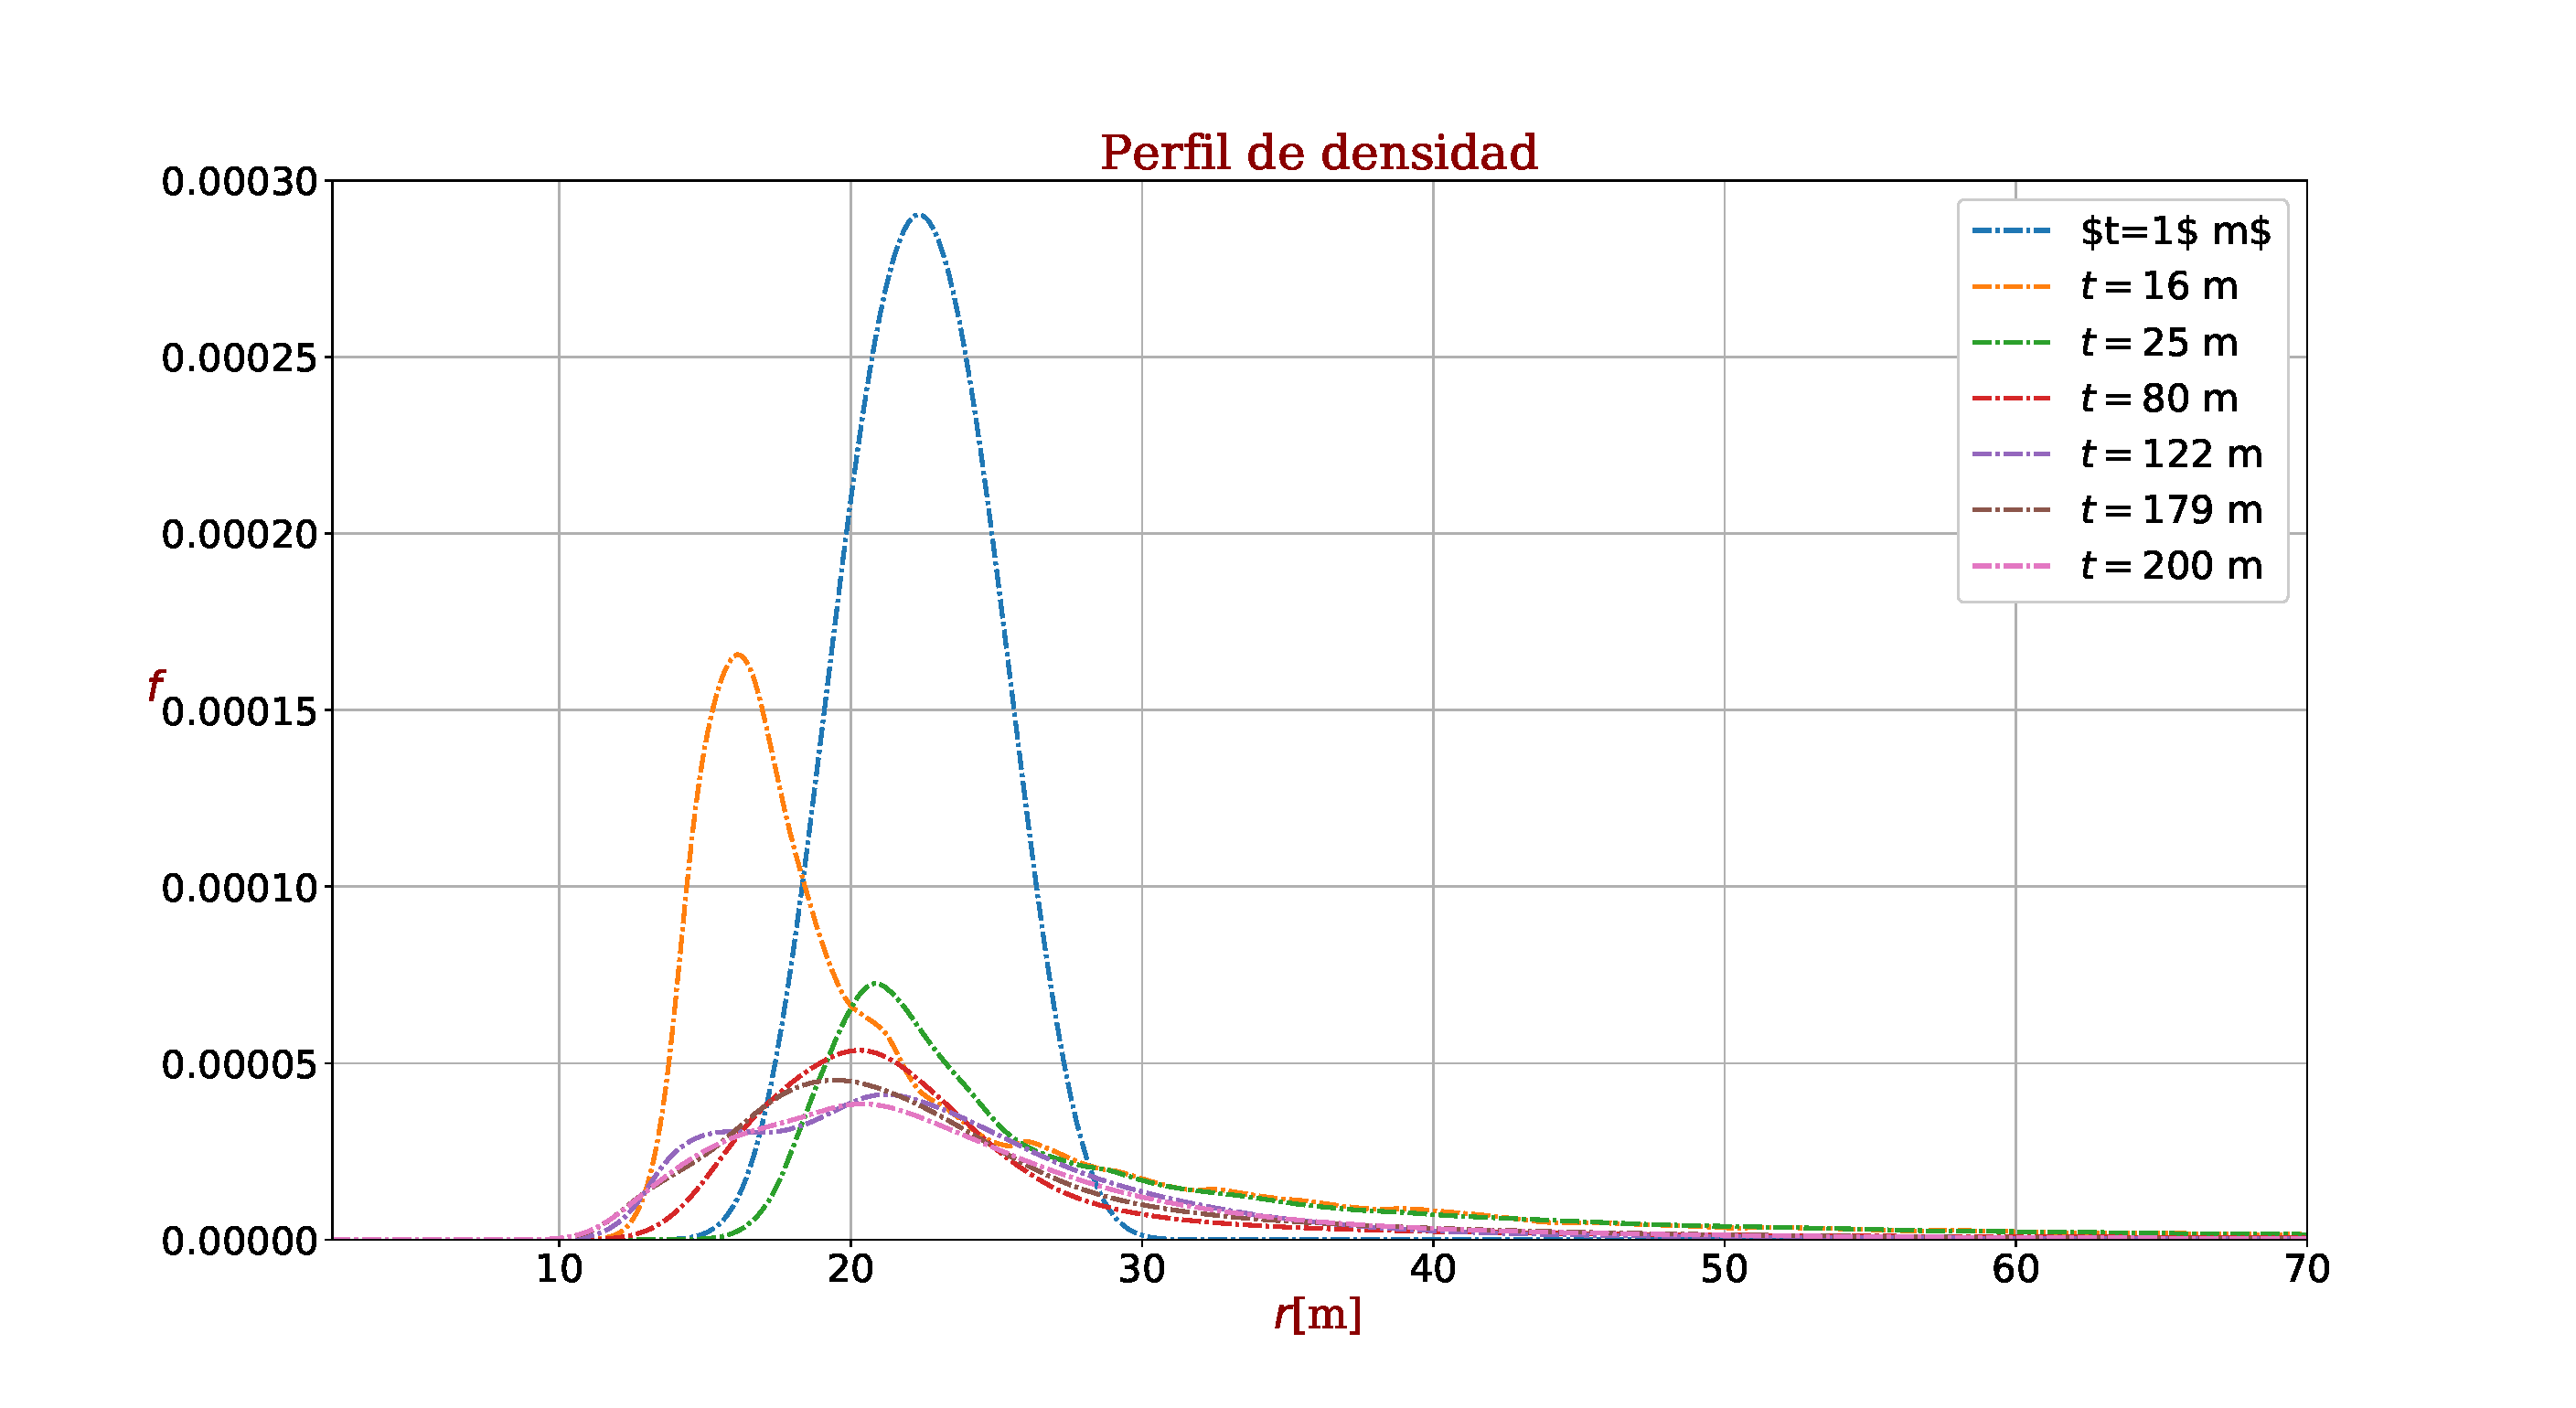
\includegraphics[height=9cm]{graphs_study/LmayorSchGraphs/densityProfileLmayorSch}
	\caption{Evolución del perfil de densidad de la función de distribución con $\tilde{L}=5.06\ M$, en coordenadas de Schwarzschild. En las gráficas se observa que una gran parte de las partículas se queda alrededor de $r_c=22.13\ \text{m}$.}
	\label{densityProfileSchLmayor}
\end{figure}

\begin{figure}[H]
	\centering
	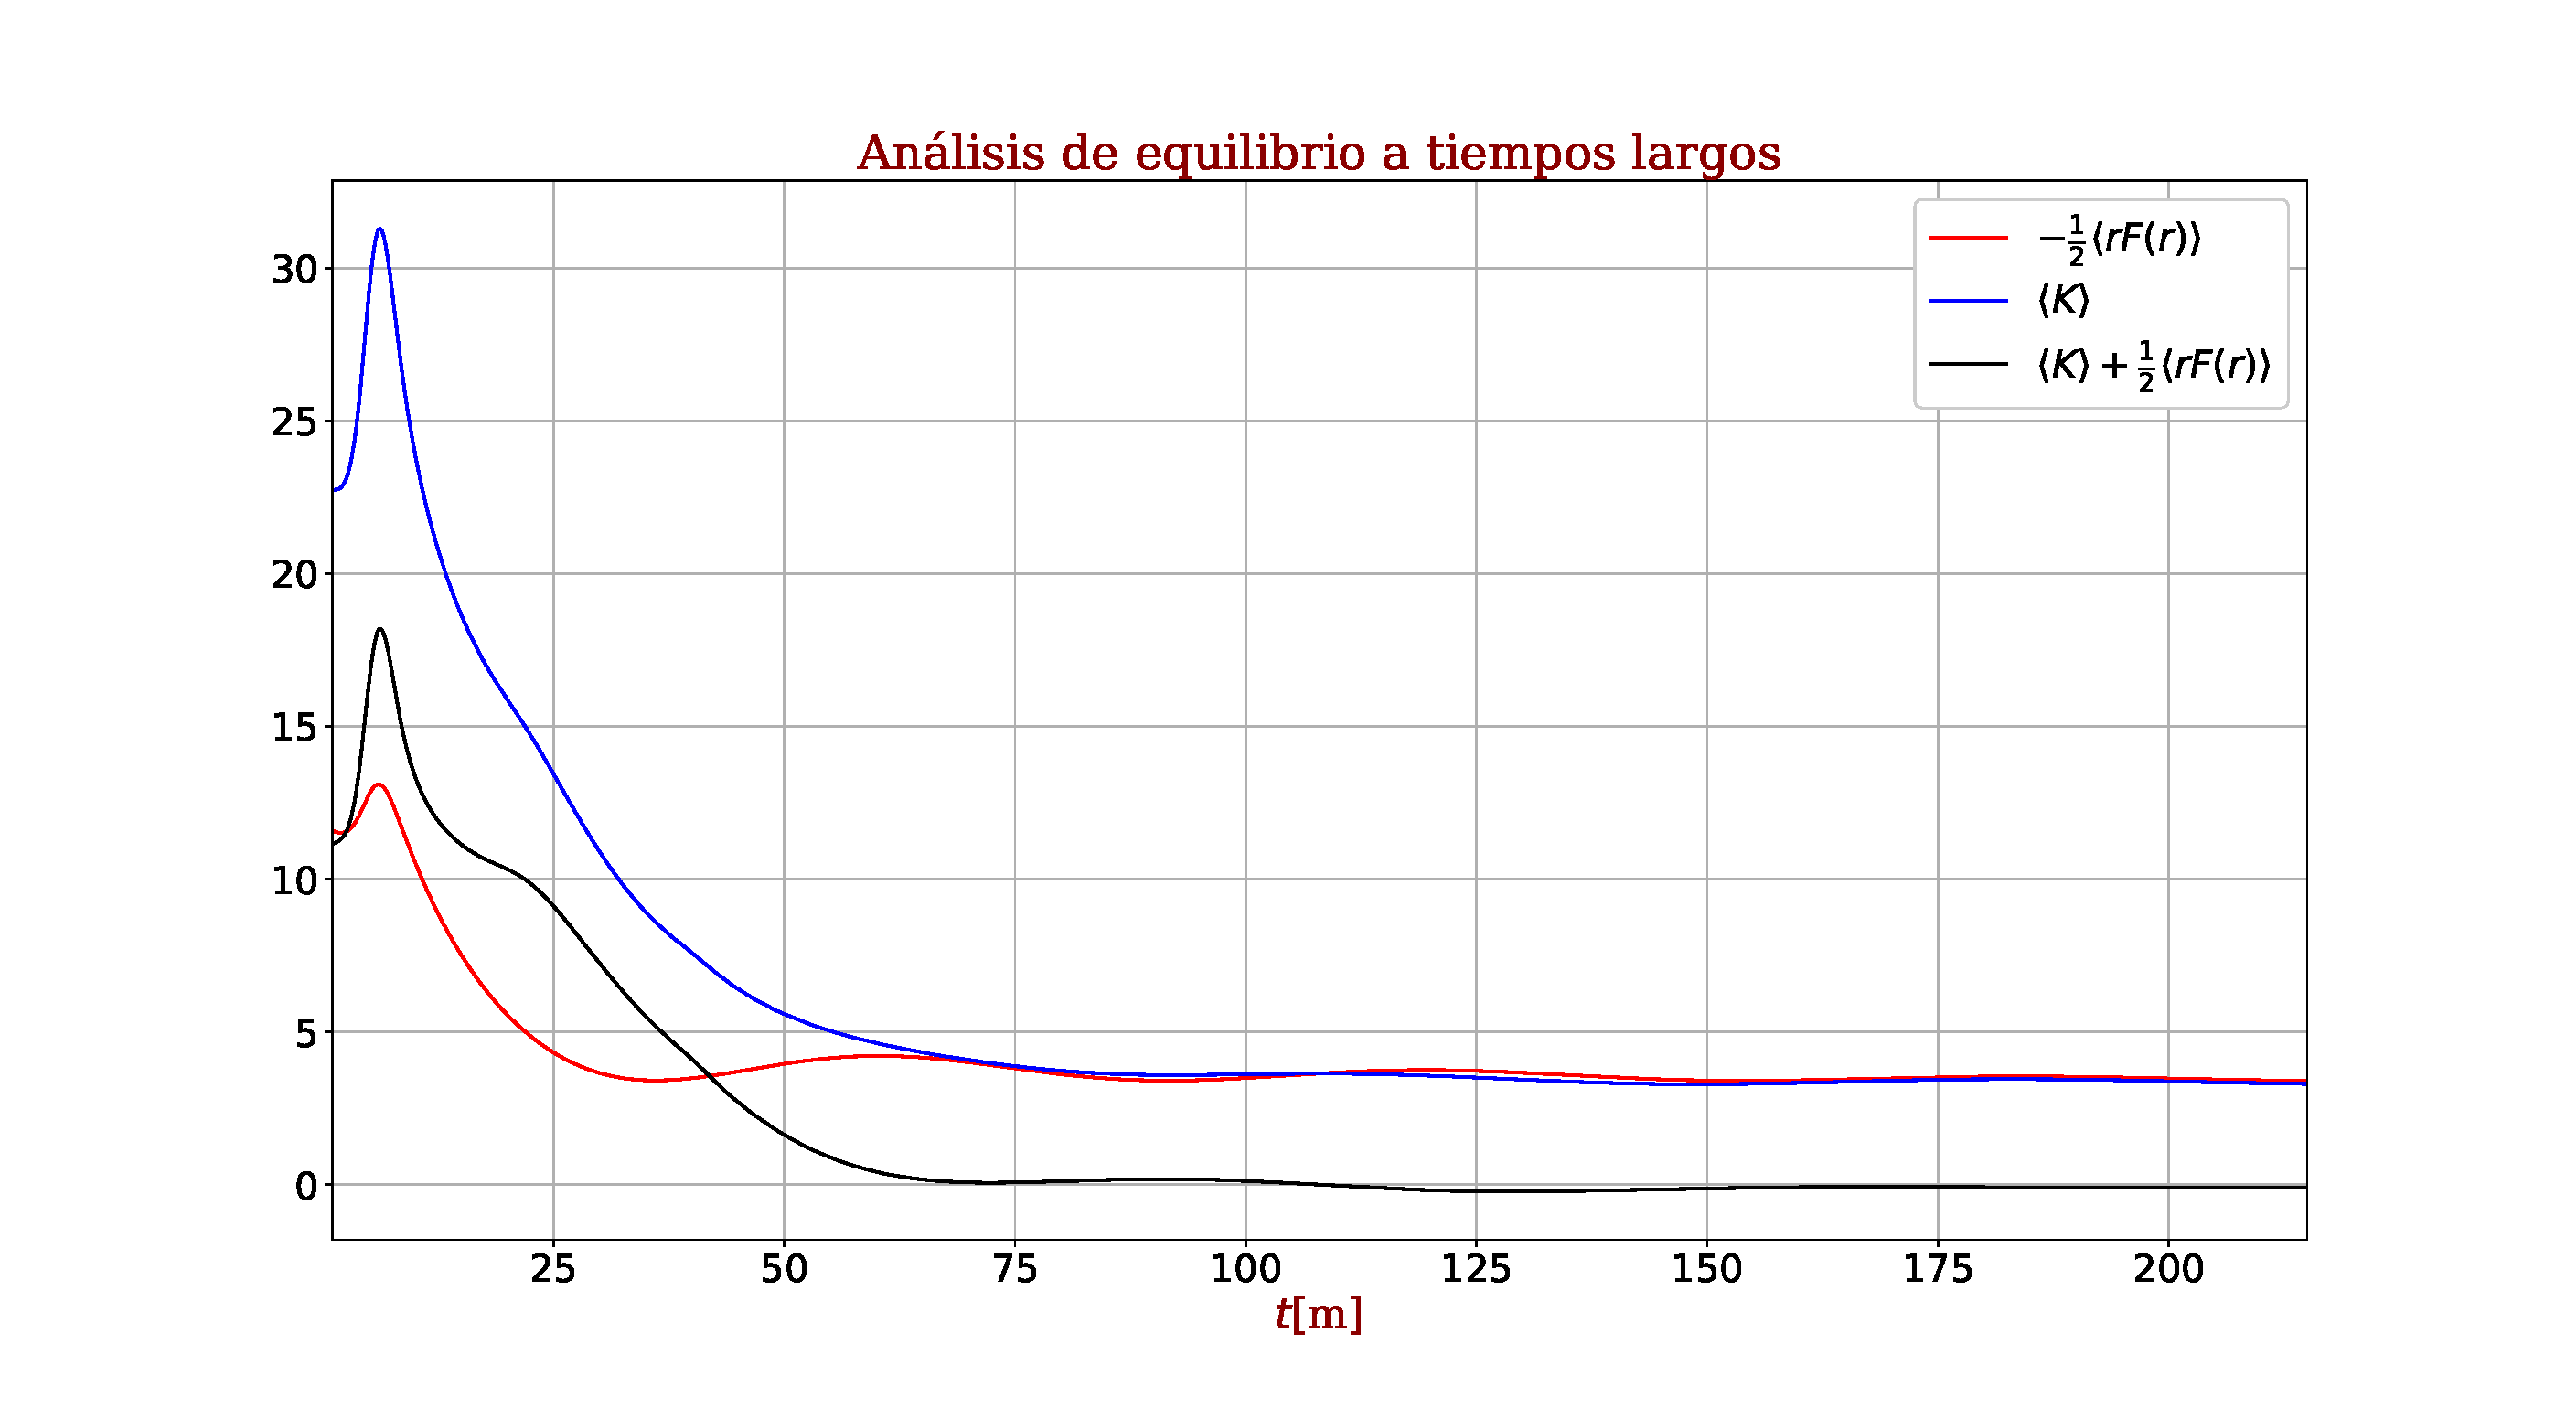
\includegraphics[height=9cm]{graphs_study/LmayorSchGraphs/stabilitySchMayor.eps}
	\caption{Análisis de equilibrio a tiempos largos. En la gráfica se muestra el promedio del virial $\frac{1}{2}\left<rF(r)\right>$ y de la energía cinética total $\left<K\right>$ para $\tilde{L}=5.06\ M$, en coordenadas de Schwarzschild. En un estado estable, ambas gráficas deberían superponerse, lo cual sucede en un tiempo determinado. Esto es de esperarse, después de que algunas partículas salen del dominio computacional, las que quedan orbitan alrededor de $r_c$ y se mantienen ahí.}
	\label{stabilitySchmayor}
\end{figure}

\begin{figure}[H]
	\centering
	\includegraphics[height=9cm]{graphs_study/LmayorSchGraphs/numpartSchMayor.eps}
	\caption{Evolución del número de partículas para $\tilde{L}=5.06\ M$, en coordenadas de Schwarzschild. Al principio, la gráfica se mantiene constante, sin embargo, a un cierto tiempo algunas partículas salen del dominio computacional. Posterioremente, el número de partículas vuelve a ser constante, en cuanto la función de distribución comienza a moverse cerca de la órbita circular estable y las partículas dejan de salir del dominio.}
	\label{numpartSchMayor}
\end{figure}

\begin{figure}[H]
	\centering
	\subfloat[]{\label{}\includegraphics[width=0.8\textwidth]{graphs_study/LmayorSchGraphs/convergencetestSchMayor1}}	
	
	\subfloat[]{\label{}\includegraphics[width=0.8\textwidth]{graphs_study/LmayorSchGraphs/convergencetestSchMayor2}}
	\caption{Análisis de convergencia a diferentes tiempos de la evolución.}
	\label{convergenceschLmayor}
\end{figure}

\newpage
\begin{figure}[H]
	\centering
	\includegraphics[width=\textwidth,height=\textheight,keepaspectratio]{graphs_study/LmenorSchGraphs/evolutionSchMenor.png}
	\caption{Evolución de la función de distribución para $\tilde{L}=0.86\ M$ (es decir, $\tilde{L}<\sqrt{12}\ M$) en distintos tiempos en coordenadas de Schwarzschild. En todas las gráficas se observa que la función no llega a la pared $r=2\ M$, por lo que nunca penetra el horizonte de eventos, sin embargo, se acercan infinitamente a él. El color representa el valor de la función de distribución en cada punto.}
	\label{evolutionLmenorSch}
\end{figure}

\begin{figure}[H]
	\centering
	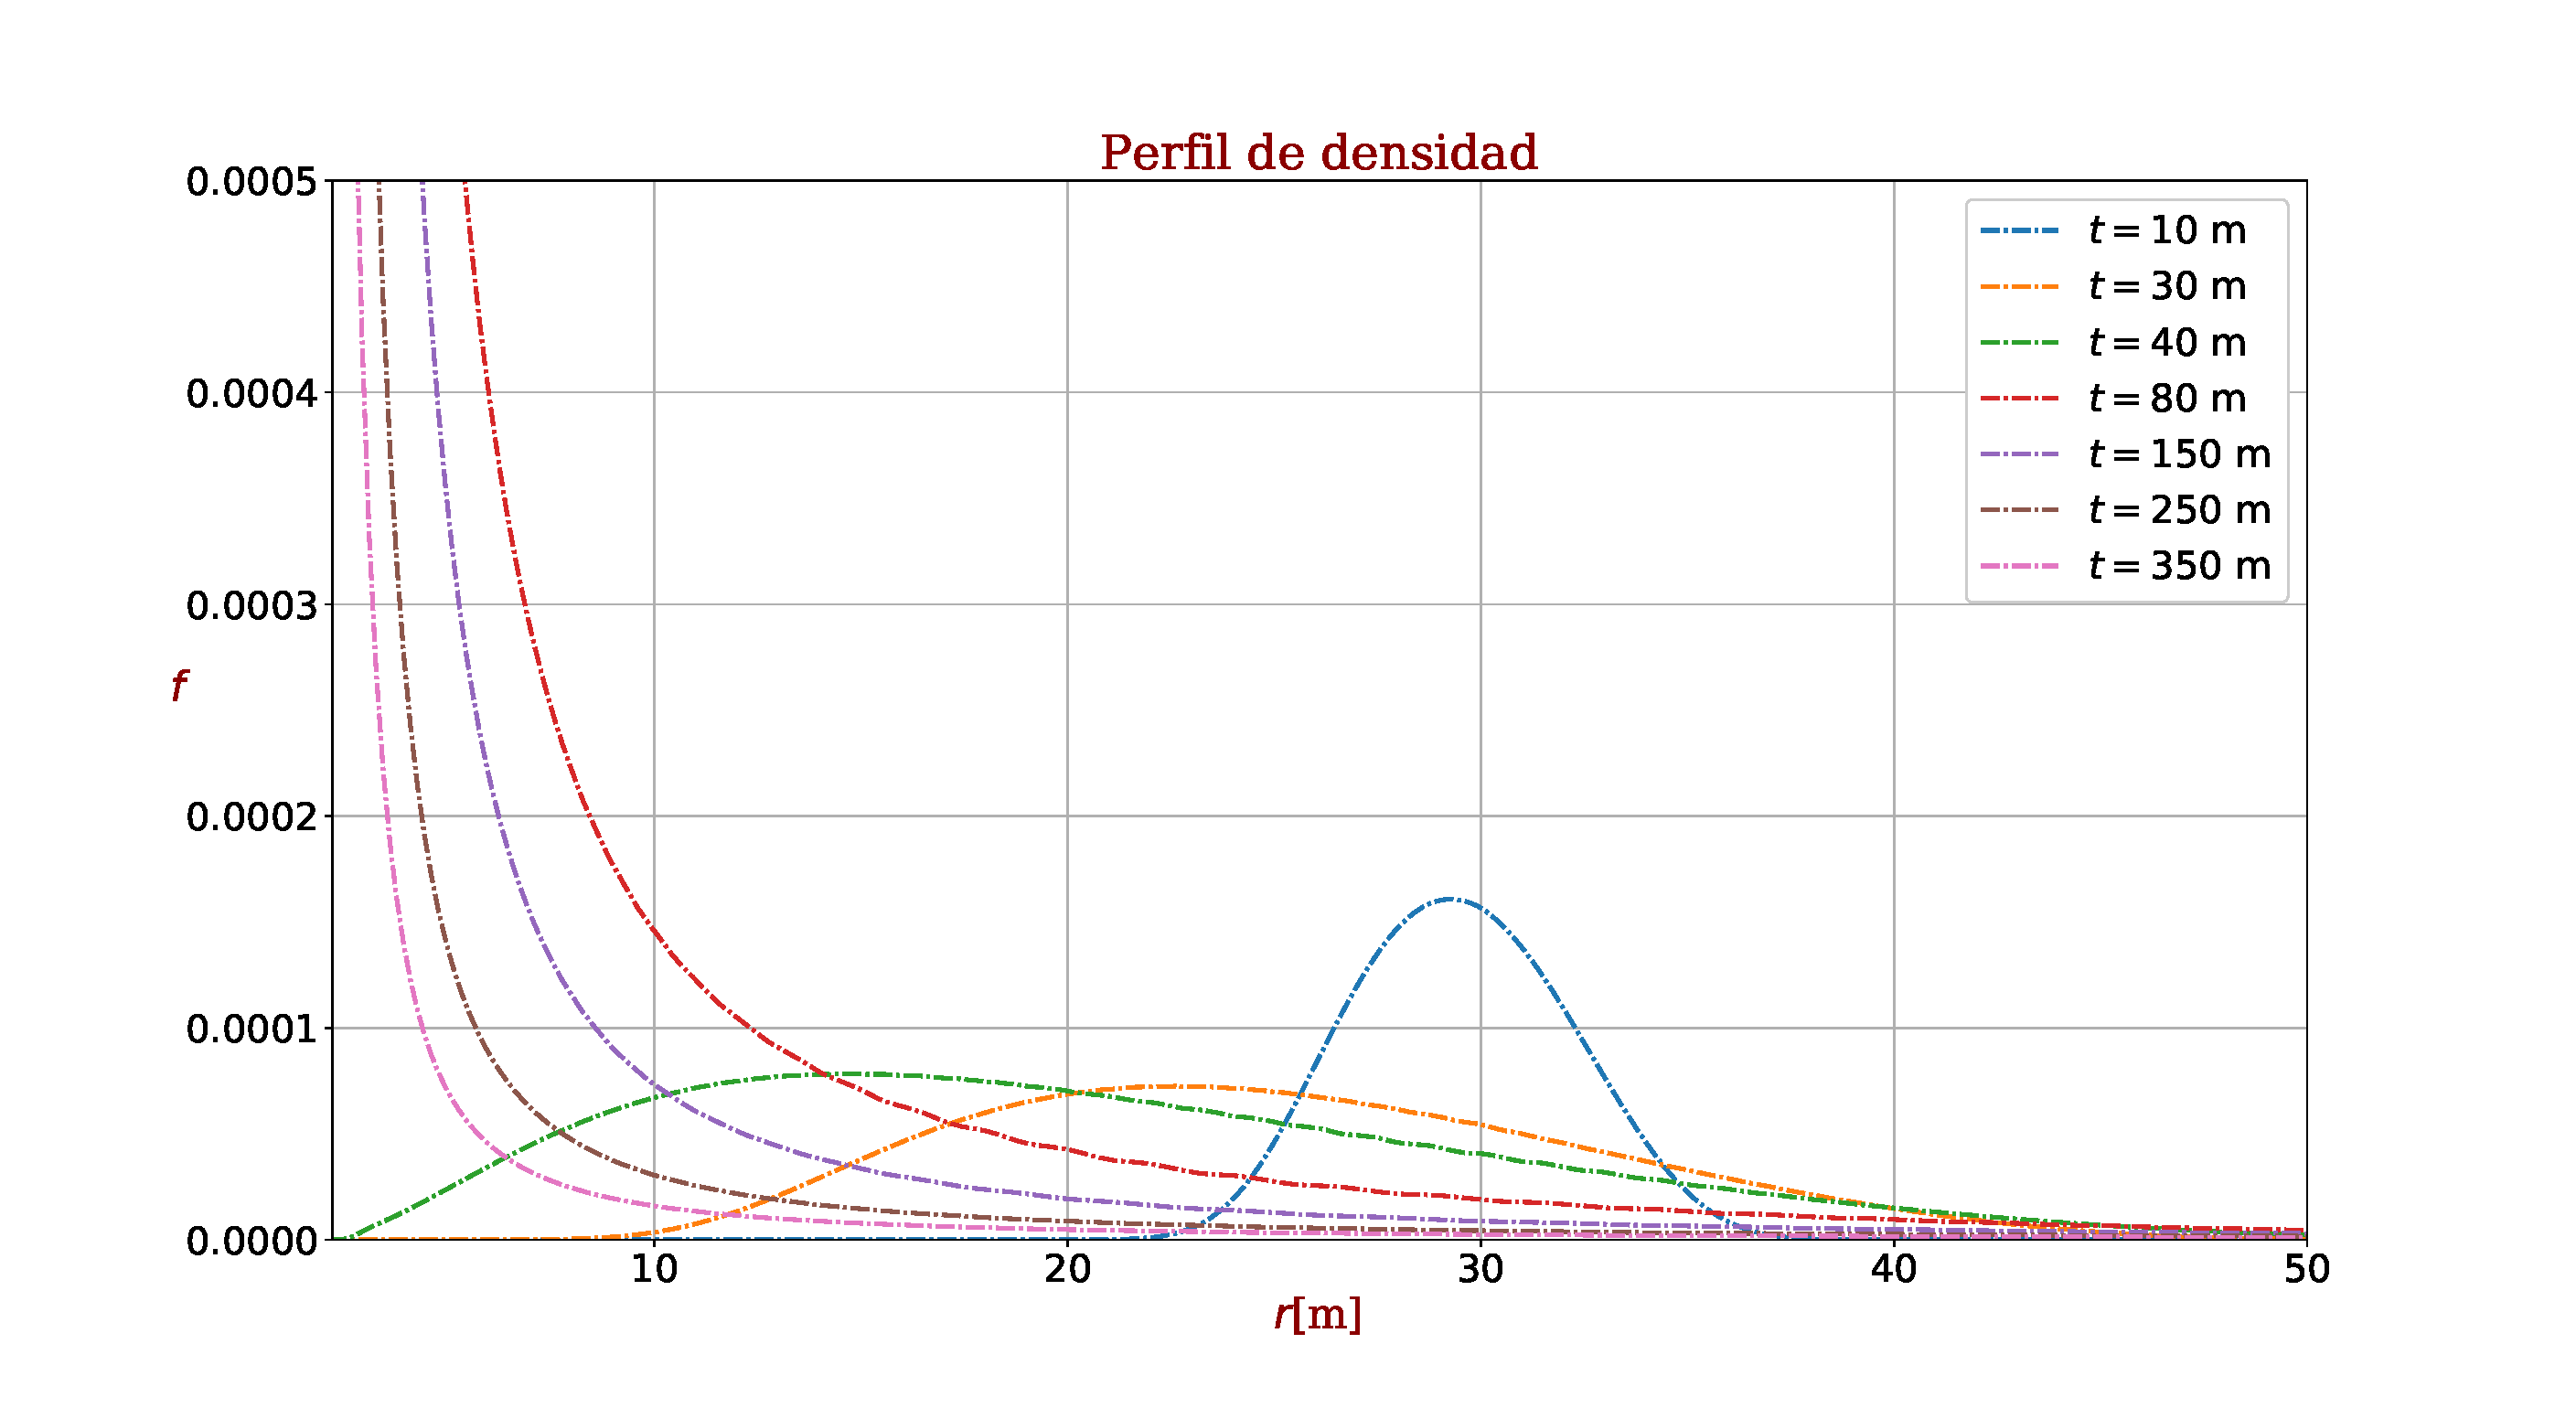
\includegraphics[height=9cm]{graphs_study/LmenorSchGraphs/densityProfileLmenorSch}
	\caption{Evolución del perfil de densidad de la función de distribución con $\tilde{L}=0.86\ M$, en coordenadas de Schwarzschild. En estas gráficas se puede ver que en un principio, la función de distribución se incrementa su anchura y disminuye su amplitud. Después, se acerca al límite $r=2\ M$ sin llegar a tocarlo, y su amplitud tiende a infinito a medida que se acerca.}
	\label{densityProfileSchLmenor}
\end{figure}

\begin{figure}[H]
	\centering
	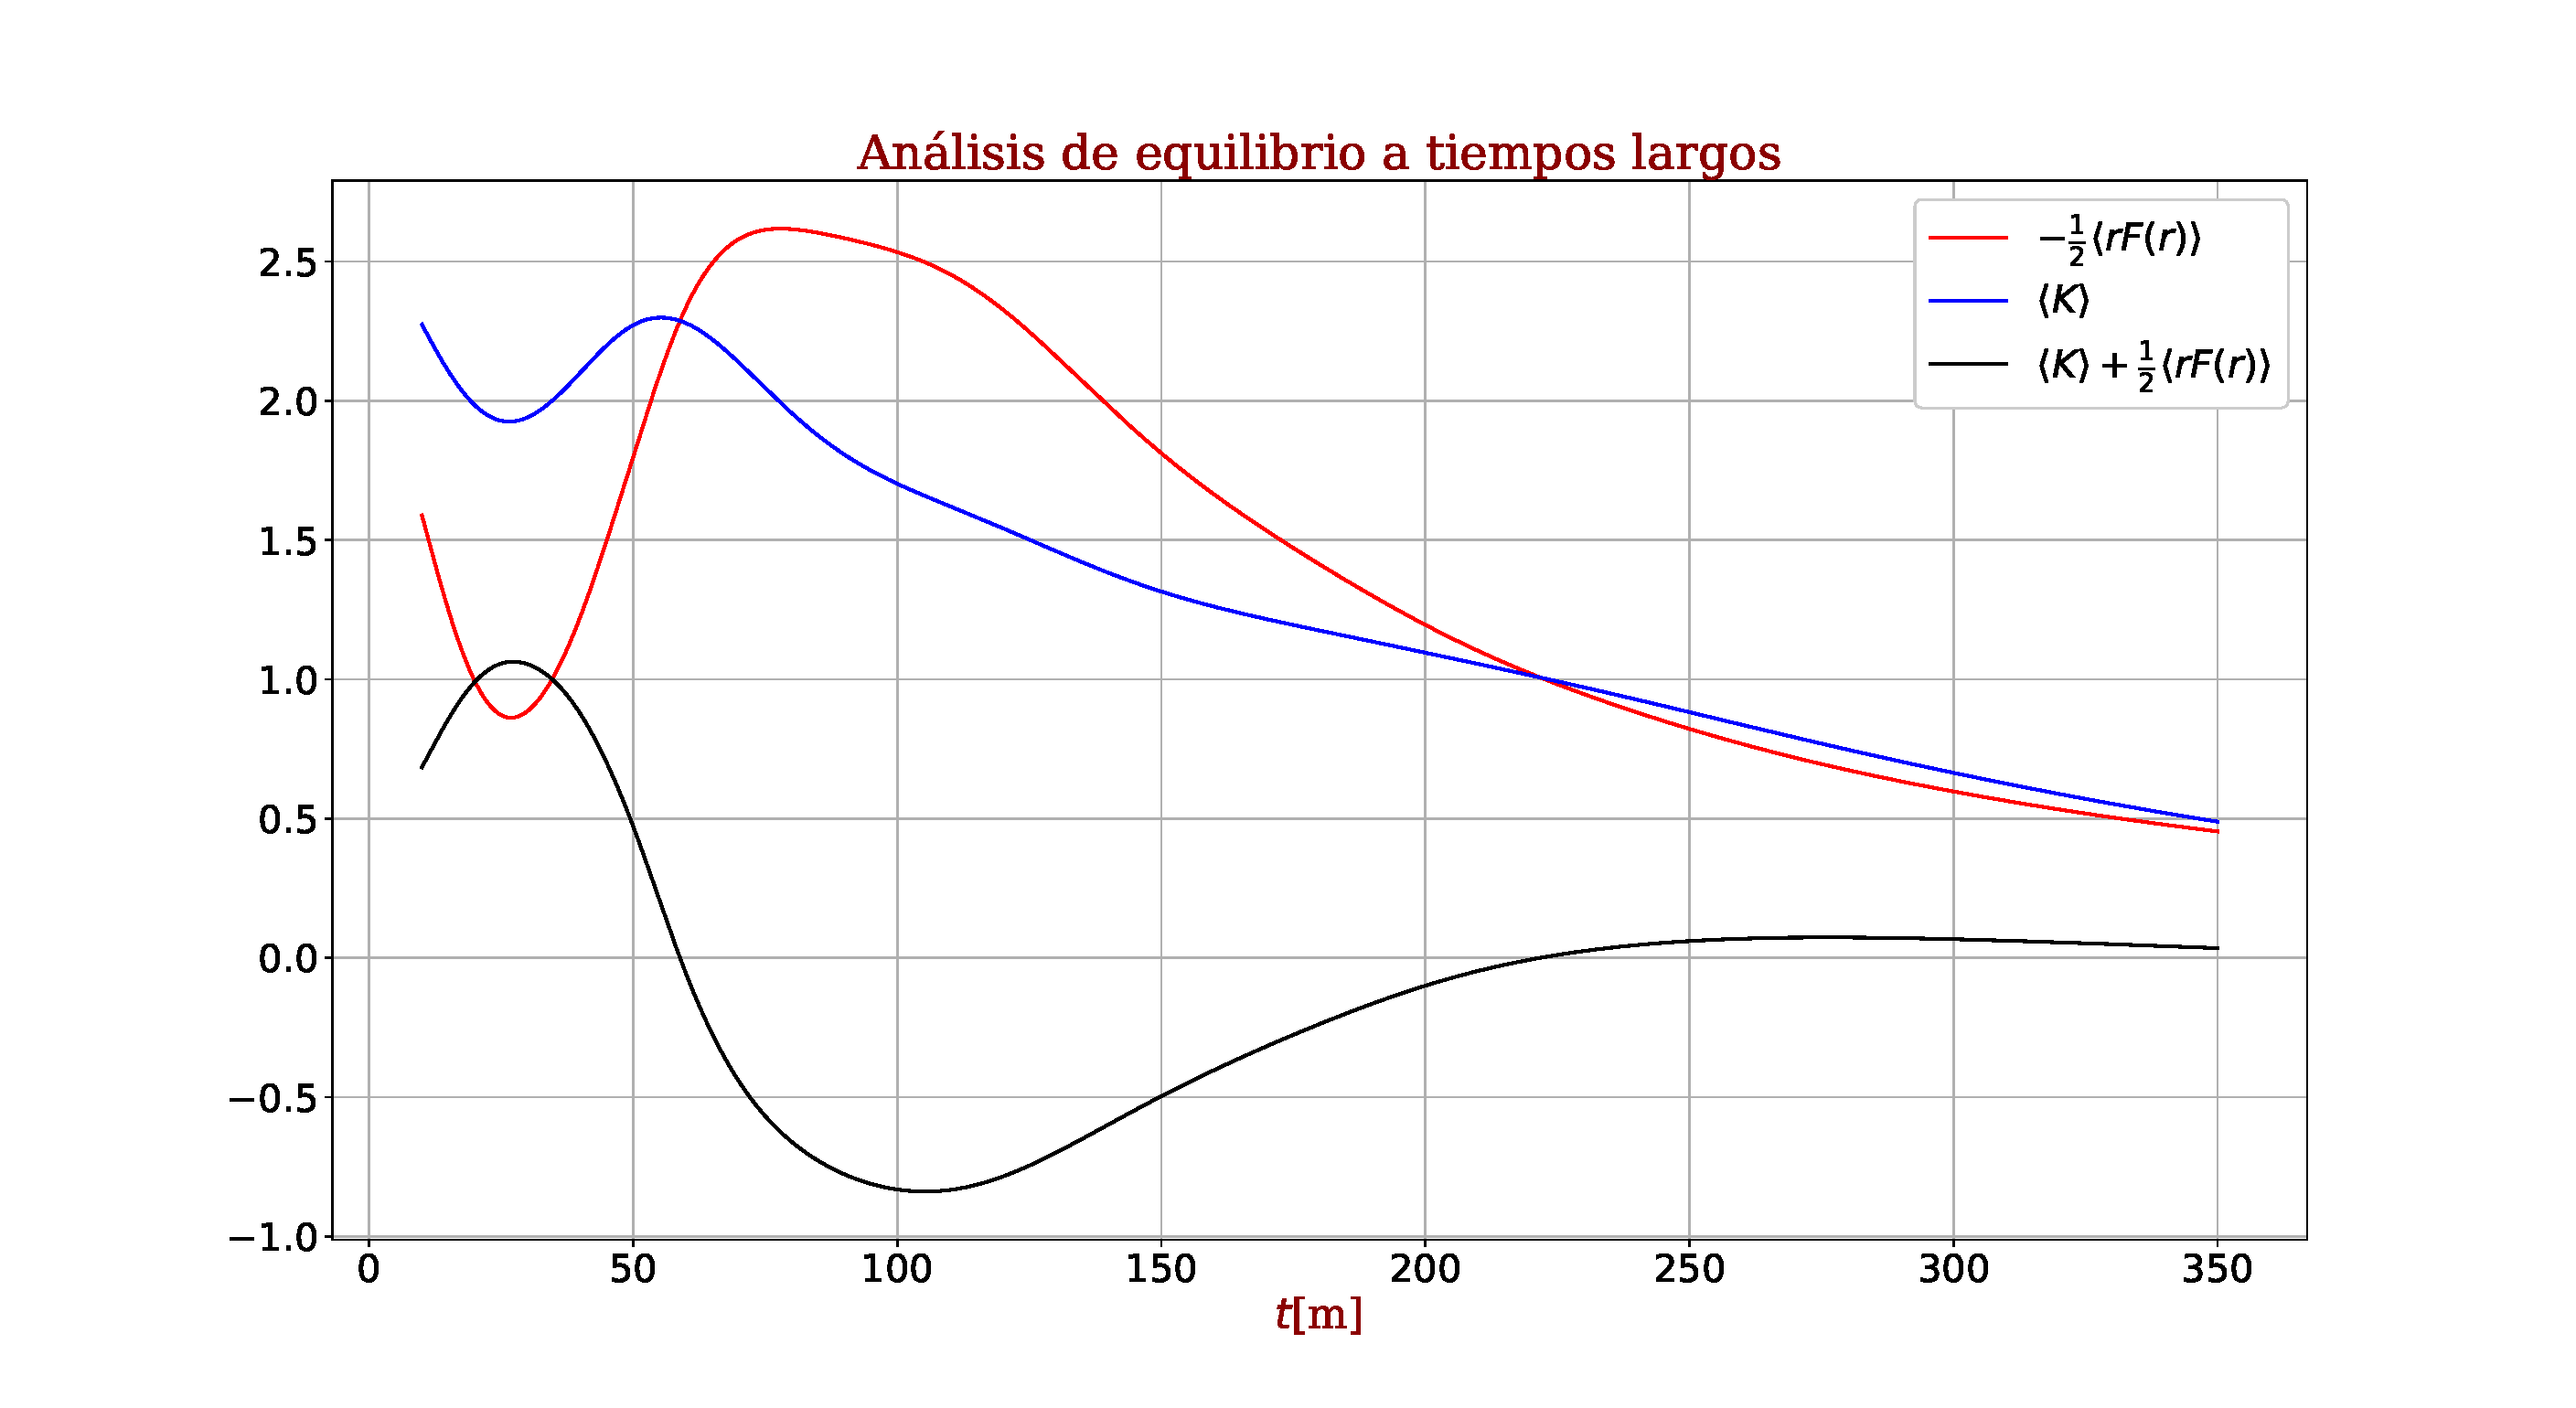
\includegraphics[height=8.5cm]{graphs_study/LmenorSchGraphs/stabilitySchMenor.eps}
	\caption{Análisis de equilibrio a tiempos largos. En la gráfica se muestra el promedio del virial $\frac{1}{2}\left<rF(r)\right>$ y de la energía cinética total $\left<K\right>$ para $\tilde{L}=0.86\ M$, en coordenadas de Schwarzschild. En un estado estable, ambas gráficas deberían superponerse, lo cual no sucede nunca perfectamente. Sin embargo, la gráficas no se separan tanto. Esto es de esperarse, ya que las partículas no dejan de tender al límite $r=2\ M$, por lo que nunca sucederá que dos gráficas sean totalmente iguales.}
	\label{stabilitySchmenor}
\end{figure}

\begin{figure}[H]
	\centering
	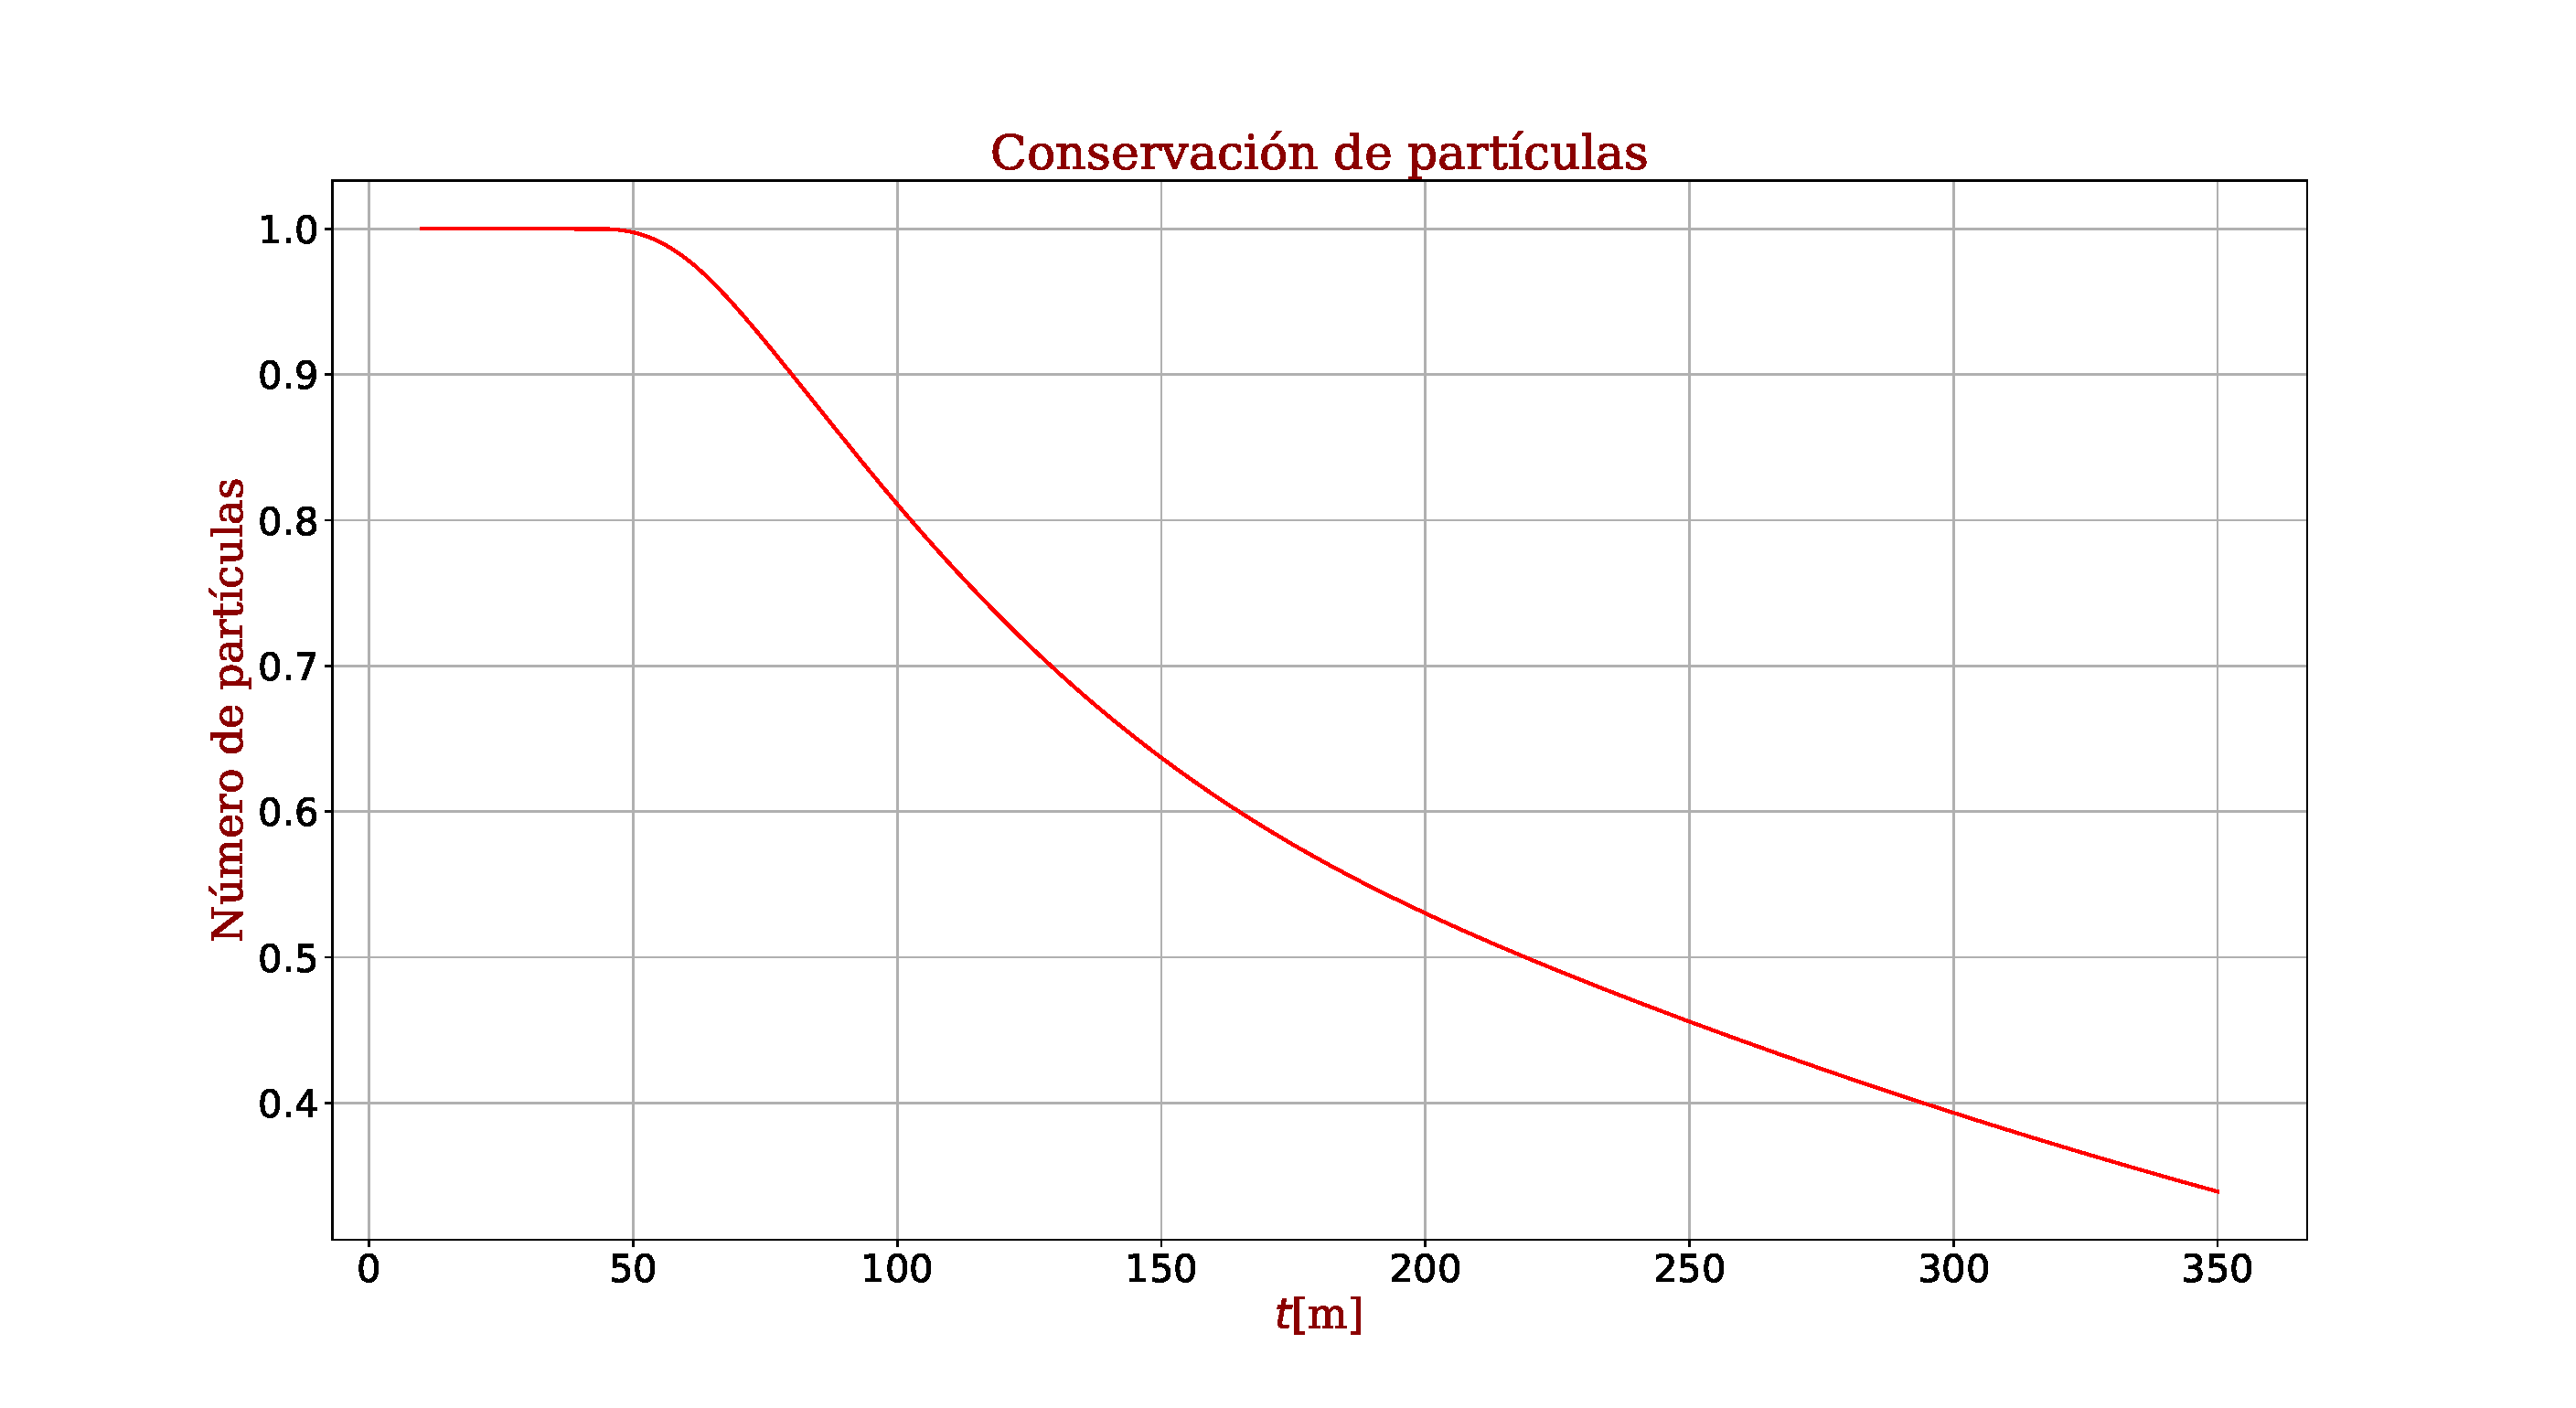
\includegraphics[height=8.5cm]{graphs_study/LmenorSchGraphs/numpartSchMenor.eps}
	\caption{Evolución del número de partículas para $\tilde{L}=0.86\ M$, en coordenadas de Schwarzschild. Al principio, la gráfica se mantiene constante. A un cierto tiempo algunas partículas comienzan a salir del dominio computacional en la frontera interna $r=2.1 M$ y no se detienen, por lo que nunca se llega realmente a un estado totalmente estable, como ya se mencionó.}
	\label{numpartSchmenor}
\end{figure}


\begin{figure}[H]
	\centering
	\subfloat[]{\label{}\includegraphics[width=0.8\textwidth]{graphs_study/LmenorSchGraphs/convergencetestSchMenor1}}	
	
	\subfloat[]{\label{}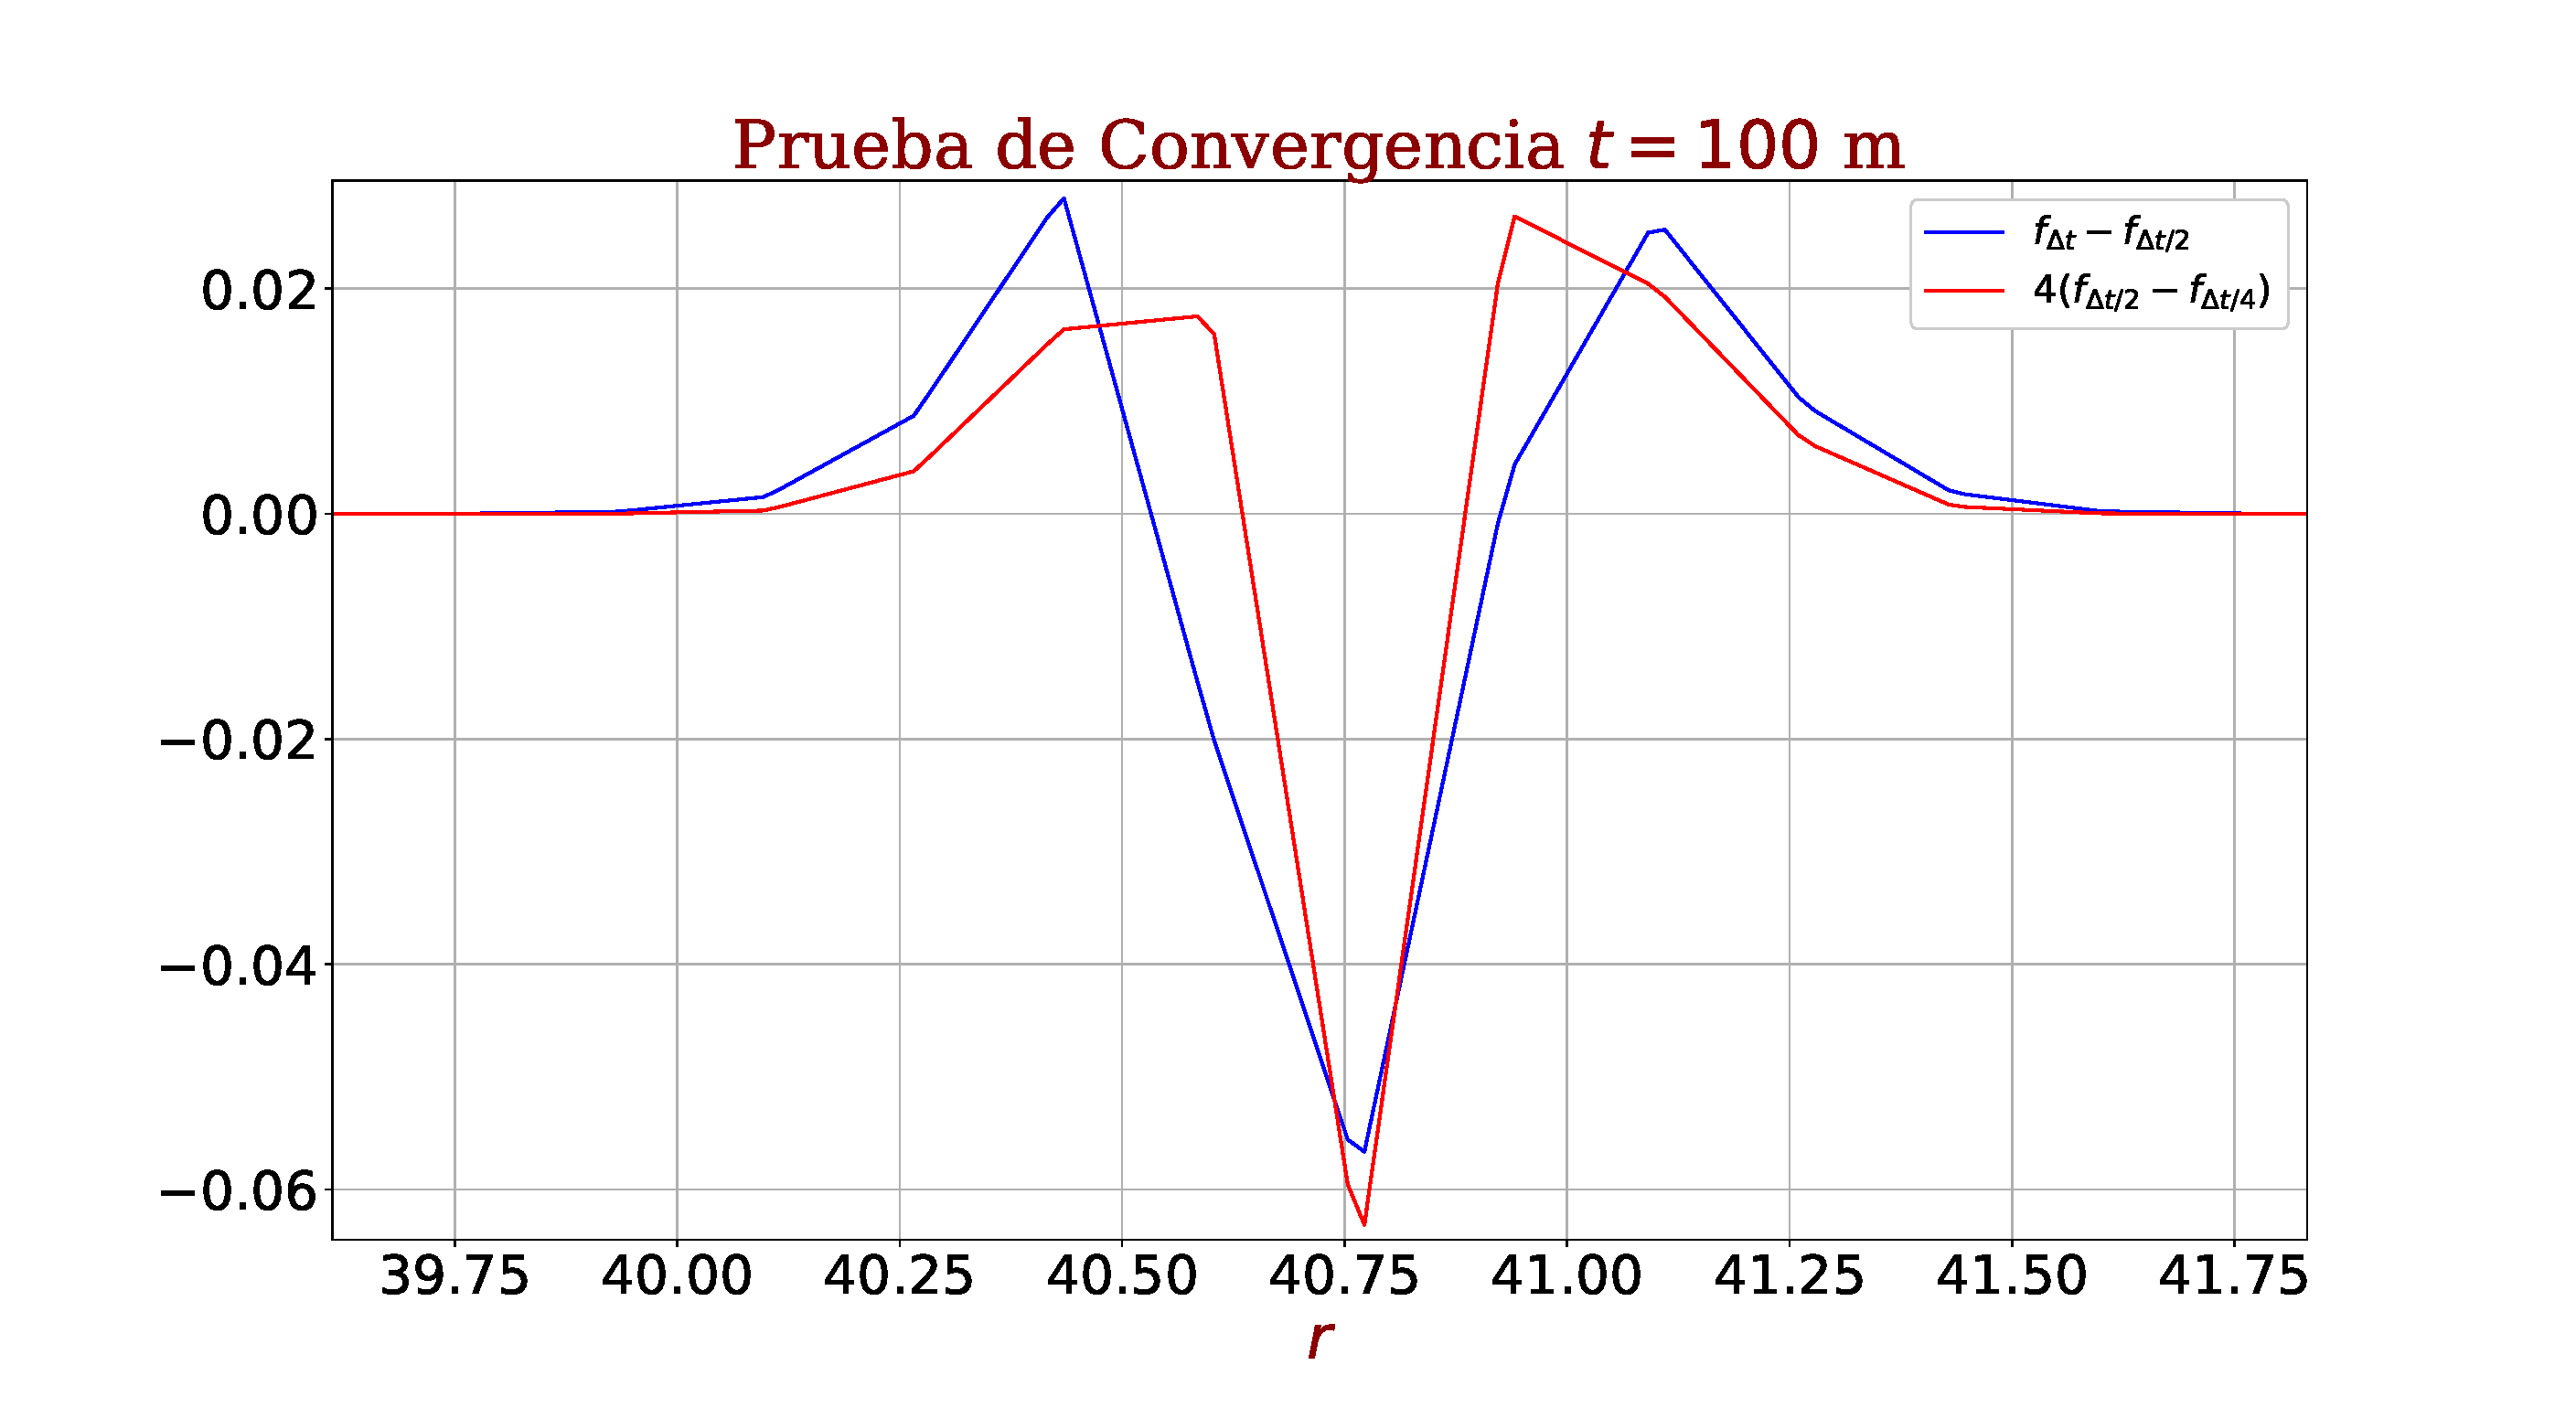
\includegraphics[width=0.8\textwidth]{graphs_study/LmenorSchGraphs/convergencetestSchMenor2}}
	
	\subfloat[]{\label{}\includegraphics[width=0.8\textwidth]{graphs_study/LmenorSchGraphs/convergencetestSchMenor3}}
	\caption{Análisis de convergencia a diferentes tiempos de la evolución.}
	\label{convergenceschLmenor}
\end{figure}

\section{Coordenadas de Kerr-Schild}

La métrica en las coordenadas de Kerr-Schild toma su forma de realizar el siguiente cambio a la coordenada temporal
\begin{equation}
\tilde{t}=t+2M\ln\abs{\frac{r}{2M}-1}
\end{equation}
de esta manera, el elemento de línea se convierte en
\begin{equation}
\text{d}S^2=-\left(1-\frac{2M}{r}\right)\ \text{d}\tilde{t}^2+\frac{4M}{r}\ \text{d}\tilde{t}\ \text{d}r+\left(1+\frac{2M}{r}\right)\ \text{d}r^2+r^2\ \left(\text{d}\theta^2+\sin^2\theta\text{d}\phi^2\right)
\end{equation}
El inverso de esta métrica se puede escribir como
\begin{equation}
g^{\alpha\beta}\partial_\alpha\partial_\beta=-\left(1+\frac{2M}{r}\right)\partial_t^2+\frac{4M}{r}\partial_t\partial_r+\left(1-\frac{2M}{r}\right)\partial_r^2+\frac{1}{r^2}\partial_\theta^2+\frac{1}{r^2\sin^2\theta}\partial_\phi^2
\end{equation}
En estas coordenadas, se observa que las cantidades 3+1 son las siguientes
\begin{equation}
\alpha=\left(1+\frac{2M}{r}\right)^{-\frac{1}{2}}, \hspace{0.4cm}A=\left(1+\frac{2M}{r}\right), \hspace{0.4cm}\beta_r=\frac{2M}{r},
\hspace{0.4cm}\beta^r=\frac{\frac{2M}{r}}{1+\frac{2M}{r}}, \hspace{0.4cm}B=\psi=1
\end{equation}
Nuevamente, dado que la métrica no depende ni de $t$ ni de $\phi$, existen vectores de Killing $\kappa^\mu$ tales que, definiendo $p^\mu=\text{d}x^\mu/\text{d}\lambda$ análogo al caso en coordenadas de Schwarzschild, $\kappa^\mu p_\mu$ es una cantidad conservada. Considerando la dirección temporal dada por $\kappa^\mu=\left(1,0,0,0\right)$, se tiene, para esta métrica
\begin{align}
g_{\mu\nu}\kappa^\mu p^\nu=g_{tt}\kappa^tp^t+g_{tr}\kappa^tp^r=g_{t\mu}p^\mu=-\left(1-\frac{2M}{r}\right)p^t+\frac{2M}{r}p^r=-E=p_t=\text{const}
\end{align}
Análogamente, considerando la dirección en la coordenada $\phi$ se tiene $\kappa^\mu=(0,0,0,1)$
\begin{align}
g_{\mu\nu}\kappa^\mu p^\nu=g_{\phi\phi}\kappa^\phi p^\phi=g_{\phi\nu}p^\nu=r^2\frac{\text{d}\phi}{\text{d}\lambda}=L=p_\phi=\text{const}
\end{align}
Para simplificar las ecuaciones finales, expresamos $p_r$ en términos de $p^r$ y de $E$ de la siguiente forma
\begin{align*}
p_r&=g_{r\alpha}p^\alpha=g_{rt}p^t+g_{rr}p^r=g_{rt}g^{t\alpha}p_\alpha+g_{rr}p^r=g_{rt}g^{tt}p_t+g_{rt}g^{tr}p_r+g_{rr}p^r\\
\Rightarrow& p_r=\frac{g_{rt}g^{tt}p_t+g_{rr}p^{r}}{1-g_{rt}g^{tr}}=\frac{-\frac{2M}{r}\left(1+\frac{2M}{r}\right)p_t+\left(1+\frac{2M}{r}\right)p^r}{1-\left(\frac{2M}{r}\right)^2}=\frac{-\frac{2M}{r}\left(1+\frac{2M}{r}\right)p_t+\left(1+\frac{2M}{r}\right)p^r}{\left(1-\frac{2M}{r}\right)\left(1+\frac{2M}{r}\right)}\\
\Rightarrow& p_r=\left(1-\frac{2M}{r}\right)^{-1}\left(p^r+\frac{2M}{r}E\right)
\end{align*}
Usando ahora la condición de normalización $g^{\mu\nu}p_\mu p_\nu=-m^2$, se tiene
\begin{align*}
-m^2&=g^{tt}p_tp_t+2g^{tr}p_tp_r+g^{rr}p_rp_r+g^{\phi\phi}p_\phi p_\phi\\
&=-\left(1+\frac{2M}{r}\right)E^2-\frac{4M}{r}Ep_r+\left(1-\frac{2M}{r}\right)p_r^2+\frac{L^2}{r^2}\\
&=p_r\left[\left(1-\frac{2M}{r}\right)p_r-\frac{4M}{r}E\right]-\left(1+\frac{2M}{r}\right)E^2+\frac{L^2}{r^2}\\
&=\left(1-\frac{2M}{r}\right)^{-1}\left(p^r+\frac{2M}{r}E\right)\left[\left(p^r+\frac{2M}{r}E\right)-\frac{4M}{r}E\right]-\left(1+\frac{2M}{r}\right)E^2+\frac{L^2}{r^2}\\
&=\left(1-\frac{2M}{r}\right)^{-1}\left[\left(p^r\right)^2-\frac{4M^2}{r^2}E^2\right]-\left(1+\frac{2M}{r}\right)E^2+\frac{L^2}{r^2}\\
\Rightarrow&\left(p^r\right)^2=E^2-\left(1-\frac{2M}{r}\right)\left(m^2-\frac{L^2}{r^2}\right)
\end{align*}
De donde se encuentra una relación idéntica a la ecuación \eqref{difenergias}, obtenida en el caso de las coordenadas de Schwarzschild 
\begin{equation}
\left(\frac{\text{d}r}{\text{d}\tau}\right)^2=\tilde{E}-\left(1+\frac{\tilde{L}^2}{r^2}\right)\left(1-\frac{2M}{r}\right)=\tilde{E}^2-V^2
\end{equation}
Se concluye que lo estudiado a partir del potencial en el caso de las coordenadas de Schwarzschild se cumple idénticamente para las coordenadas de Kerr-Schild, en particular, las cantidades dadas por las ecuaciones \eqref{rc}, \eqref{Lc} y \eqref{Ec} son las mismas.

\subsection{Resultados numéricos}
\noindent
En la tabla \ref{datosks} se muestran las cantidades utilizadas para cada simulación. Nuevamente, para el análisis de convergencia se tomo un espaciamiento $\Delta t$ y se hicieron tres simulaciones, con $\Delta t$, $\Delta t/2$ y $\Delta t/4$. Los momentos angulares utilizados para las diferentes simulaciones fueron $\tilde{L}=3.86\ M>\sqrt{12}\ M$ y $\tilde{L}=1.16\ M<\sqrt{12}M$. Los factores de Courant $\rho_r\ \text{d}r/\text{d}t$ y $\rho_p\ \text{d}p_r/\text{d}t$, análogo al caso en coordenadas de Schwarzschild, cumplen siempre la condición \eqref{cfl}, ya que lo cumplen para los valores máximos que toman $\text{d}r/\text{d}t$ y $\text{d}p_r/\text{d}t$ en toda la malla. 

Dado que, como ya se demostró, el potencial efectivo toma la misma forma en ambas coordenadas, se utilizaron momentos angulares que, nuevamente, fueran mayores y menores a $\sqrt{12}\ M$. En este caso, fueron $\tilde{L}=3.86\ M>\sqrt{12}\ M$ y $\tilde{L}=1.16\ M<\sqrt{12}\ M$. No sé tomaron los mismos momentos que se utilizaron en coordenadas de Schwarzschild ya que estos provocaban que el tiempo de cada simulación fuera mucho más grande (por el cambio en $\text{d}p_r/\text{d}t$ debido a la expresión en coordenadas de Kerr-Schild del lapso $\alpha$, principalmente).

Nuevamente, la evolución de la función de distribución en el espacio-fase muestra un comportamiento distinto dependiendo de la magnitud del momento angular utilizado, que concuerda con la forma del potencial en estas coordenadas, es decir, en el caso cuando el momento angular es mayor a $\sqrt{12}\ M$ (figura \ref{evolutionLmayorKS}) y considerando una distribución centrada en $r_c(L)$ dada por \eqref{rc}, ninguna de las partículas cae más allá del horizonte de eventos y una buena parte de ellas orbita alrededor de $r_c$, aquellas que logran irse se debe a que tenían demasiada energía. Esto puede notarse también analizando el perfil de densidad mostrado en la figura \ref{densityProfileKSLmayor}, donde vemos que a medida que pasa el tiempo, la mayor parte de las partículas se queda en una zona alrededor de $r_c$. Comparando esta gráfica con \ref{densityProfileSchLmayor}, se puede también observar que, debido a que las partículas en el caso de las coordenadas de Kerr-Schild tienen un momento angular más pequeño que en la simulación realizada en coordenadas de Schwarzschild ($3.86\ M$ en la primera y $5.06\ M$ en la segunda), las primeras se concentran en un dominio en $r$ más reducido, lo cual es de esperarse si observamos la forma del potencial (figura \ref{schpotential}).

Cuando el momento angular es menor que $\sqrt{12}\ M$ (figura \ref{evolutionLmenorKS}), las partículas que conforman la función de distribución se acercan al horizonte de eventos y en este caso logran penetrarlo, lo cual se puede ver en la figura \ref{densityProfileKSLmenor}, donde sucede que en un principio la función de distribución se hace más ancha y pierde amplitud, pasa el horizonte de eventos, y a medida que se acerca al origen, su amplitud tiende a infinito.

En las figuras \ref{numpartKSMayor} y \ref{numpartKSMenor} se muestra el número de partículas en función del tiempo para el caso con $\tilde{L}>\sqrt{12}\ M$ y $\tilde{L}<\sqrt{12}\ M$, respectivamente. En ellas se puede notar una pérdida de partículas, sin embargo, análogo a lo visto en coordenadas de Schwarzschild, en el primer caso esta pérdida se debe únicamente a que la función de distribución comienza a salir del dominio computacional (llega un momento en que ya no hay pérdida, que es el momento en que la función se queda orbitando). En el caso $\tilde{L}<\sqrt{12}\ M$ el límite del dominio computacional se tomó en $M/4$ para evitar problemas en el origen al momento de la simulación, por lo que la pérdida de partículas se debe a que las partículas comienzan a salir de este dominio.

En las figuras \ref{stabilityKSLmayor} y \ref{stabilityKSLmenor} se muestra el análisis de equilibrio a tiempos largos para $\tilde{L}>\sqrt{12}\ M$ y $\tilde{L}<\sqrt{12}\ M$, respectivamente. Cuando el sistema llega a un estado estable, las gráficas de $\frac{1}{2}\left<rF(r)\right>$ y $\left<K\right>$ deberían superponerse. En el primer caso sí sucede, como ya se mencionó, llega un momento en que las partículas orbitan de manera estable y se quedan así, sin embargo, el tiempo que le toma llegar a un estado perfectamente estable es grande y requiere mucho tiempo computacional. Para el caso $\tilde{L}<\sqrt{12}\ M$ no se llega a un estado estable, lo cual es de esperarse debido a que la función de distribución al evolucionar se acerca infinitamente al horizonte de eventos, sin que ninguna partícula entre, por lo que no se debería llegar a la estabilidad.

Por último, se muestran los análisis de convergencia para $\tilde{L}>\sqrt{12}\ M$ (figura \ref{convergenceksLmayor}) y $\tilde{L}<\sqrt{12}\ M$ (figura \ref{convergenceksLmenor}) para distintos tiempos en la evolución. Se puede ver que, a medida que se hace el espaciamiento más pequeño, las gráficas convergen. Sin embargo, como ocurre con las coordenadas de Schwarzschild, debido a que las fórmulas en diferencias finitas suponen velocidades constantes y el orden de las fórmulas se obtiene dando esto como hipótesis, al tomar velocidades dependientes de la posición y el tiempo, nuevamente disminuyen su orden de convergencia.

\begin{table}[t]
	\centering
	\caption{Cantidades utilizadas para las simulaciones en coordenadas de Kerr-Schild, con distintos momentos angulares.}\label{datosks}
	\resizebox{0.95	\textwidth}{!}{%
		\begin{tabular}{|c||c|cccccccccc|} \hline
			\rowcolor{lightgray} Variables	&$\tilde{L}$			&$\Delta t$			&$\rho_r$	&$\rho_p$	&$M$	&$m$			&$N$	&$r_c$			&$p_c$				&$s_r$				&$s_p$				\\ \hline
			\multirow{2}{1cm}{Valores}		&$3.86\ M$			&$0.001\ \text{m}$	&$0.011$		&$0.051$		&$1\ \text{m}$		&$1\ \text{m}$	&$1$	&$10.73\ \text{m}$&$0.69\ \text{m}$	&$0.5\ \text{m}$	&$0.1\ \text{m}$	\\
			&$1.16\ M$			&$0.01\ \text{m}$	&$0.06$ 	&$0.45$ 	&$1\ \text{m}$		&$1\ \text{m}$	&$1$	&$30.0\ \text{m}$&$0.0\ \text{m}$	&$1.0\ \text{m}$	&$0.3\ \text{m}$	\\ \hline
	\end{tabular}}
\end{table}

\newpage
\begin{figure}[H]
	\centering
	\includegraphics[width=\textwidth,height=\textheight,keepaspectratio]{graphs_study/LmayorKSGraphs/evolutionKSMayor.png}
	\caption{Evolución de la función de distribución para $\tilde{L}=3.86\ M$ (es decir, $\tilde{L}>\sqrt{12}\ M$) en distintos tiempos en coordenadas de Kerr-Schild. En este conjunto de gráficas se puede apreciar de manera más importante la rotación de la función alrededor de $r_c$. El color representa el valor de la función de distribución en cada punto.}
	\label{evolutionLmayorKS}
\end{figure}

\begin{figure}[H]
	\centering
	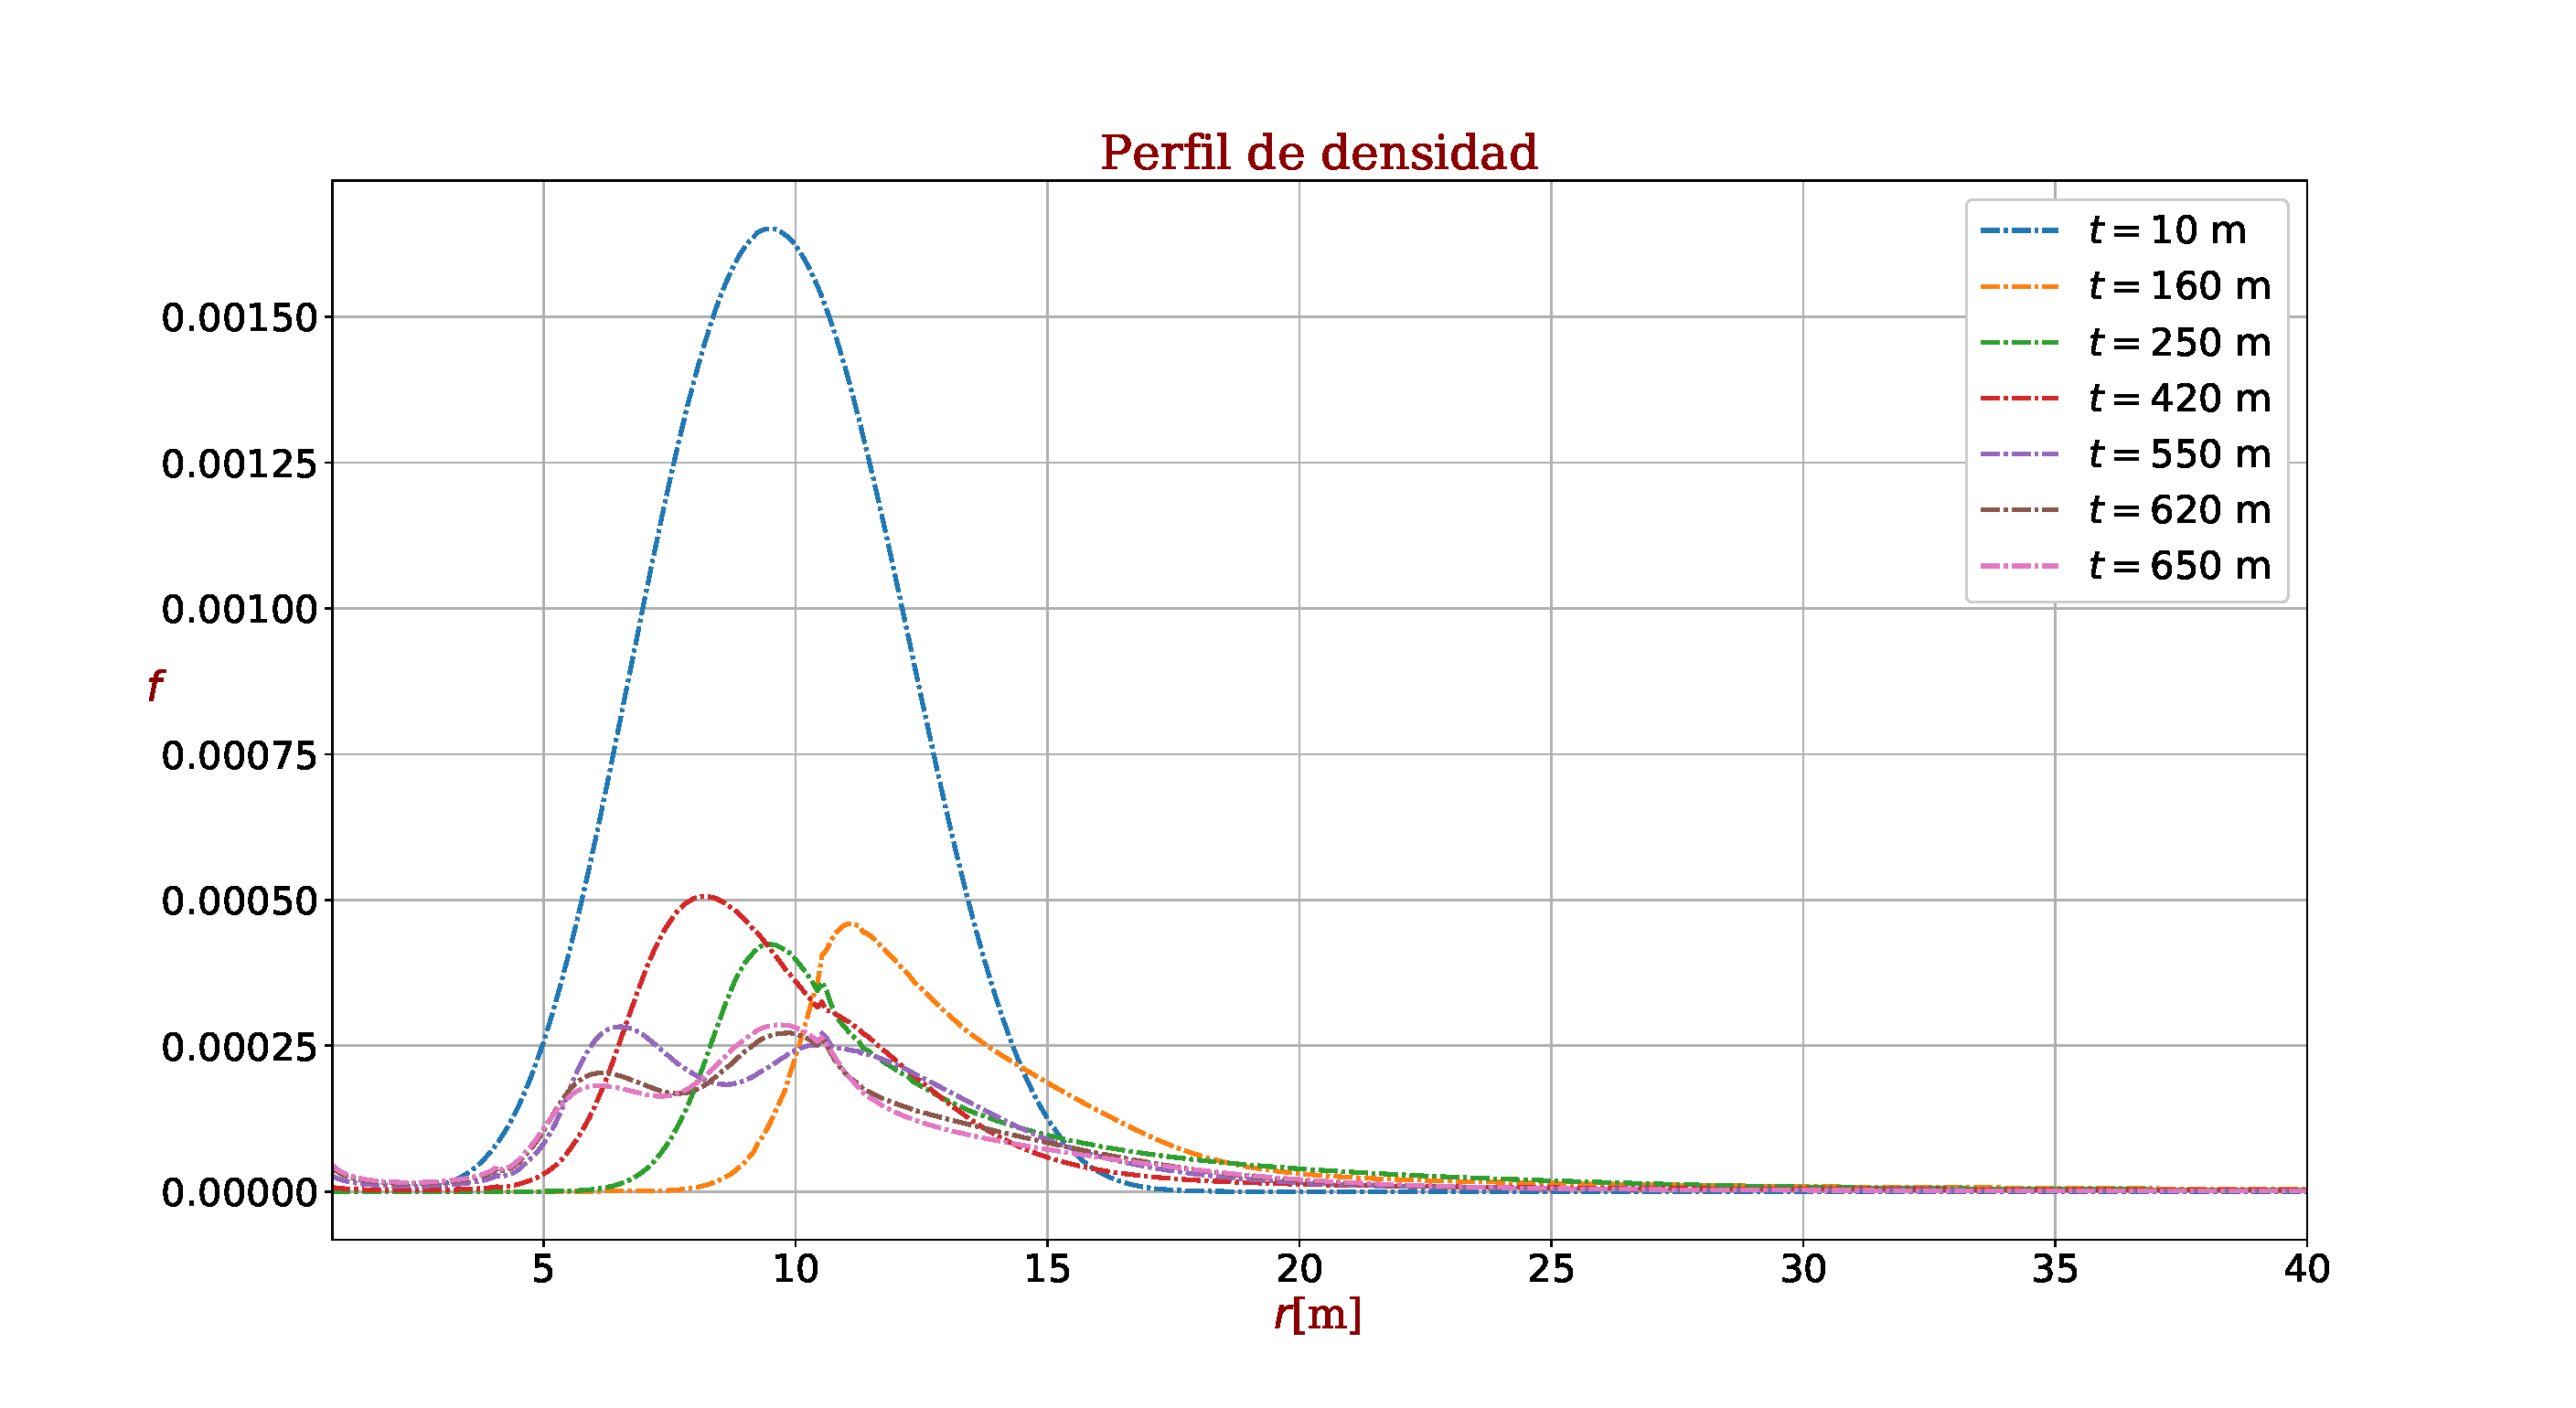
\includegraphics[height=9cm]{graphs_study/LmayorKSGraphs/densityProfileLmayorKS}
	\caption{Evolución del perfil de densidad de la función de distribución con $\tilde{L}=3.86\ M$, en coordenadas de Kerr-Schild. En las gráficas se observa que una gran parte de las partículas se queda alrededor de $r_c=10.73\ \text{m}$.}
	\label{densityProfileKSLmayor}
\end{figure}

\begin{figure}[H]
	\centering
	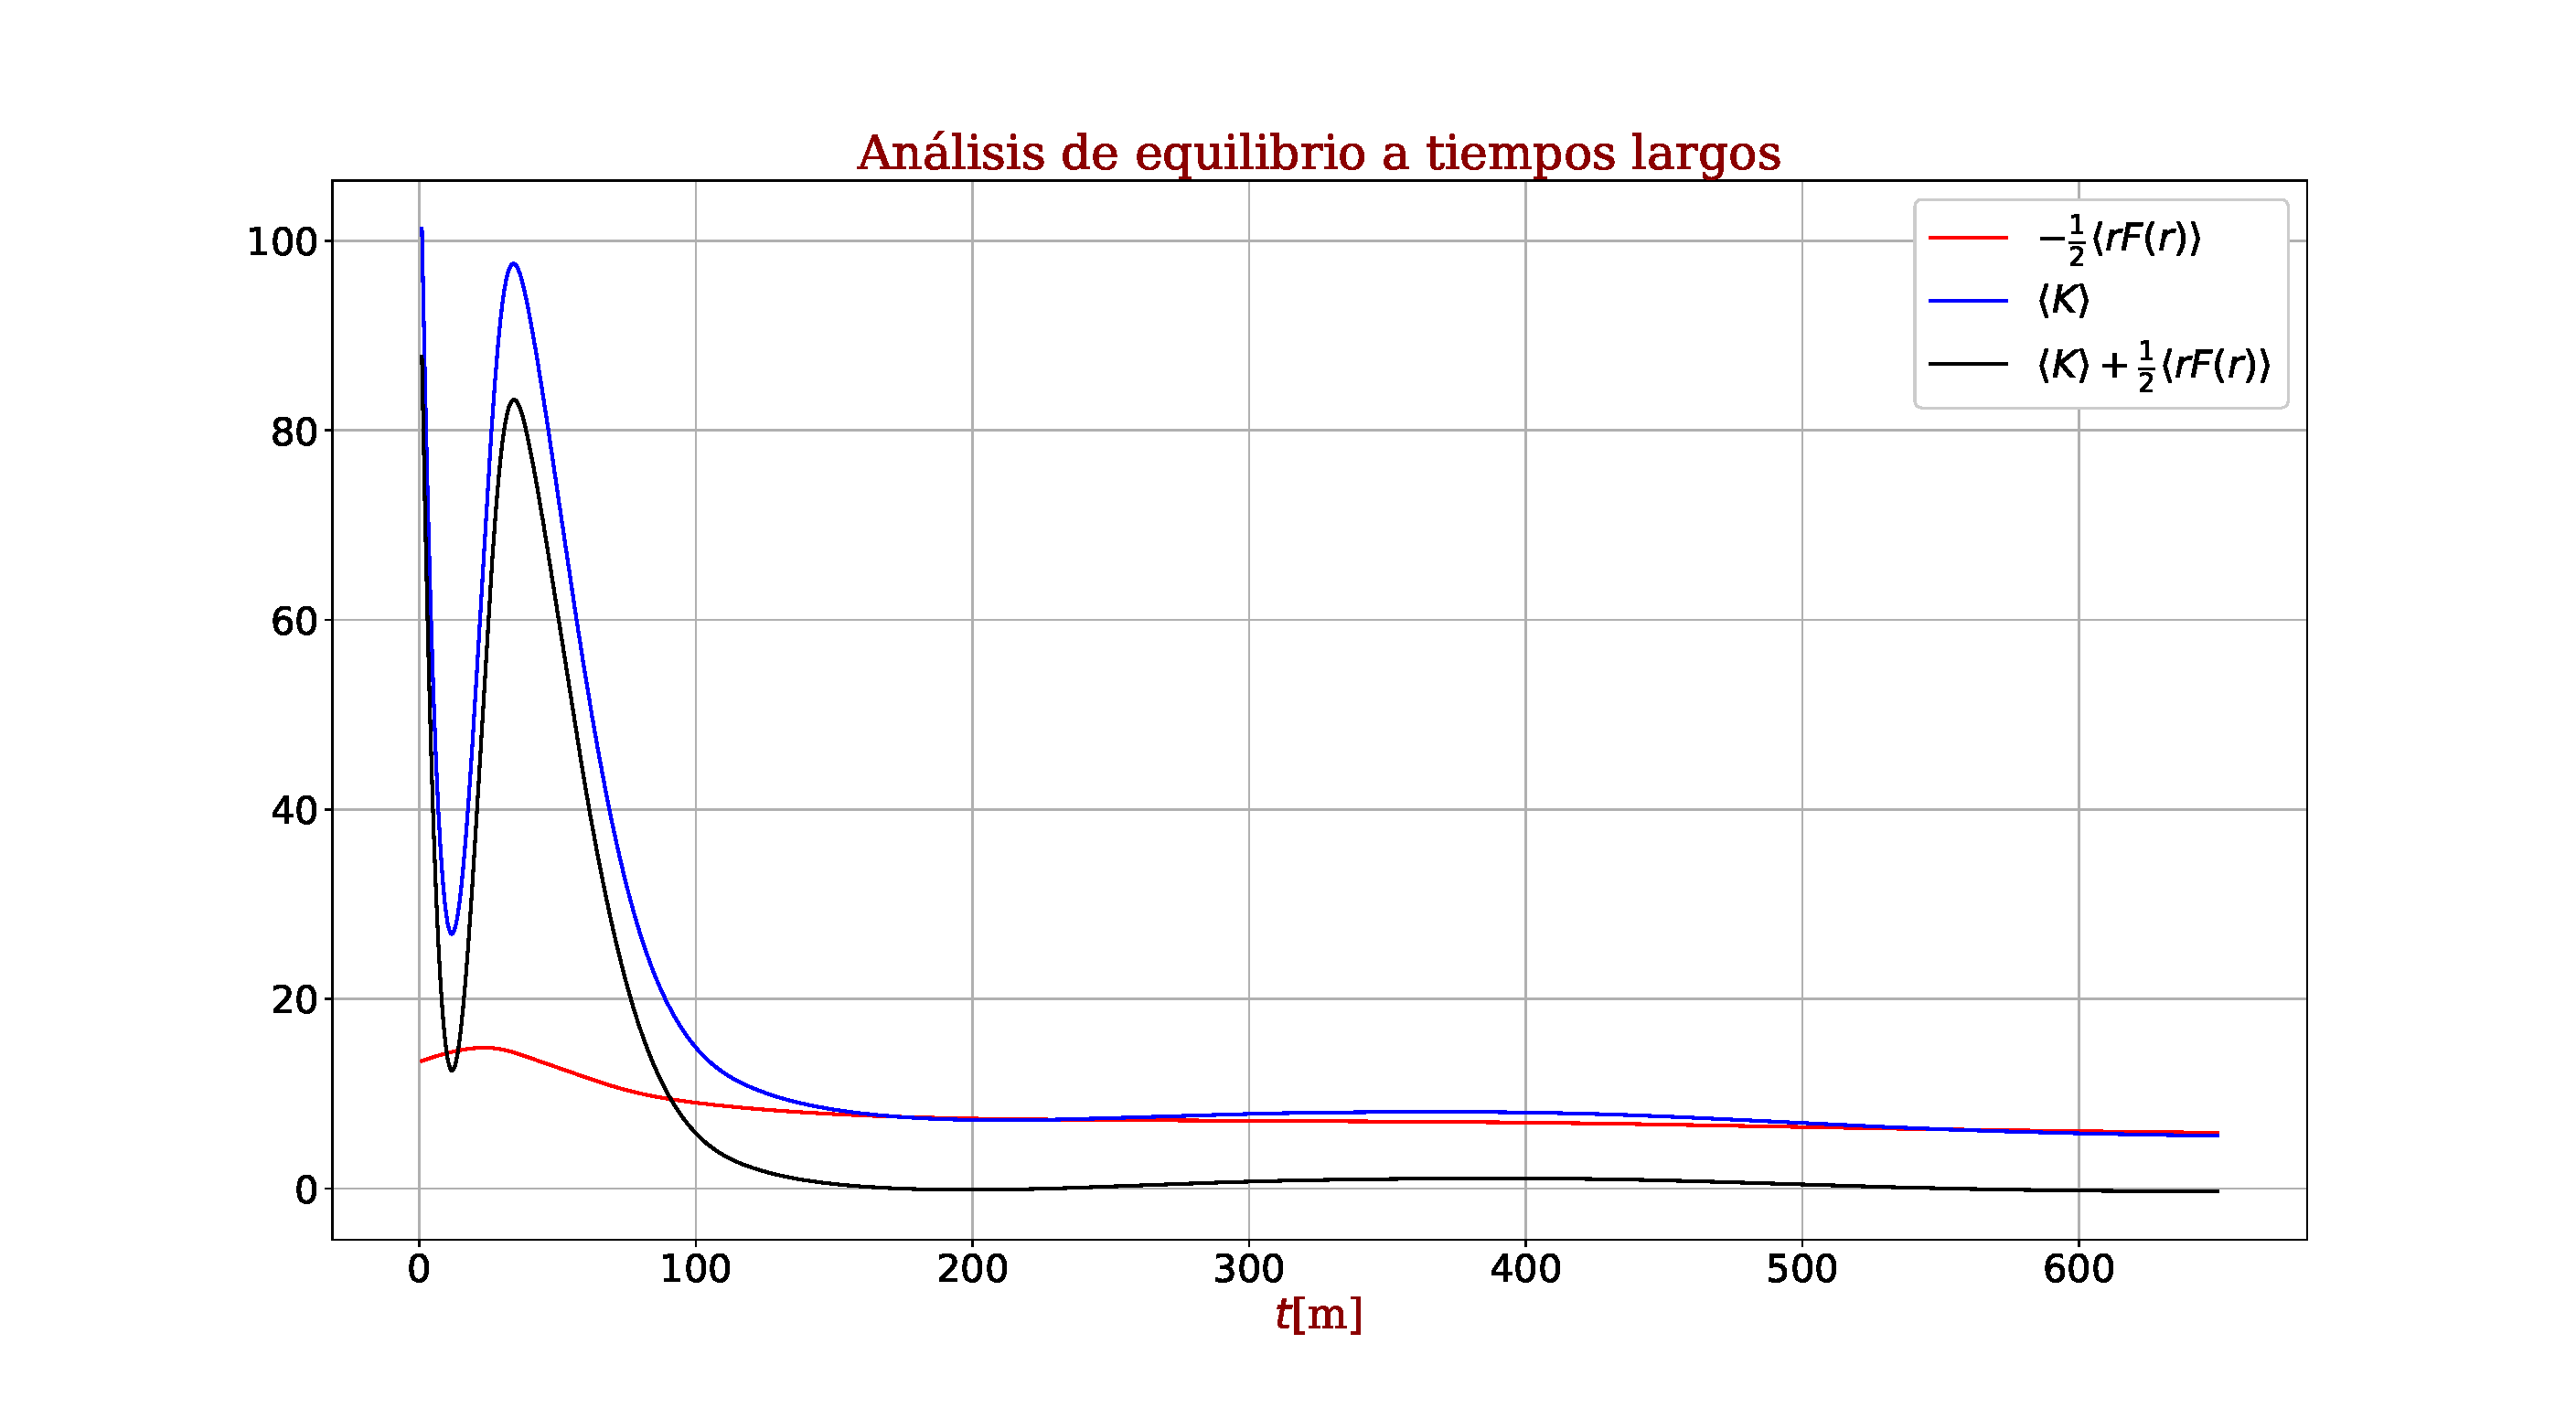
\includegraphics[height=9cm]{graphs_study/LmayorKSGraphs/stabilityKSMayor.eps}
	\caption{Análisis de equilibrio a tiempos largos. En la gráfica se muestra el promedio del virial $\frac{1}{2}\left<rF(r)\right>$ y de la energía cinética total $\left<K\right>$ para $\tilde{L}=3.86\ M$, en coordenadas de Kerr-Schild. En un estado estable, ambas gráficas deberían superponerse, lo cual sucede en un tiempo determinado. Esto es de esperarse, después de que algunas partículas salen del dominio computacional, las que quedan orbitan alrededor de $r_c$ y se mantienen ahí.}
	\label{stabilityKSLmayor}
\end{figure}

\begin{figure}[H]
	\centering
	\includegraphics[height=9cm]{graphs_study/LmayorKSGraphs/numpartKSMayor.eps}
	\caption{Evolución del número de partículas para $\tilde{L}=3.86\ M$, en coordenadas de Kerr-Schild. Notamos que desde un principio existe pérdida de partículas, lo que indica que la evolución fue más rápida y la función sale en menor tiempo. Sin embargo, a un cierto tiempo el número de partículas llega a ser constante, en cuanto la función de distribución comienza a moverse cerca de la órbita circular estable y las partículas dejan de salir del dominio.}
	\label{numpartKSMayor}
\end{figure}

\begin{figure}[H]
	\centering
	\subfloat[]{\label{}\includegraphics[width=0.8\textwidth]{graphs_study/LmayorKSGraphs/convergencetestKSMayor1}}	
	
	\subfloat[]{\label{}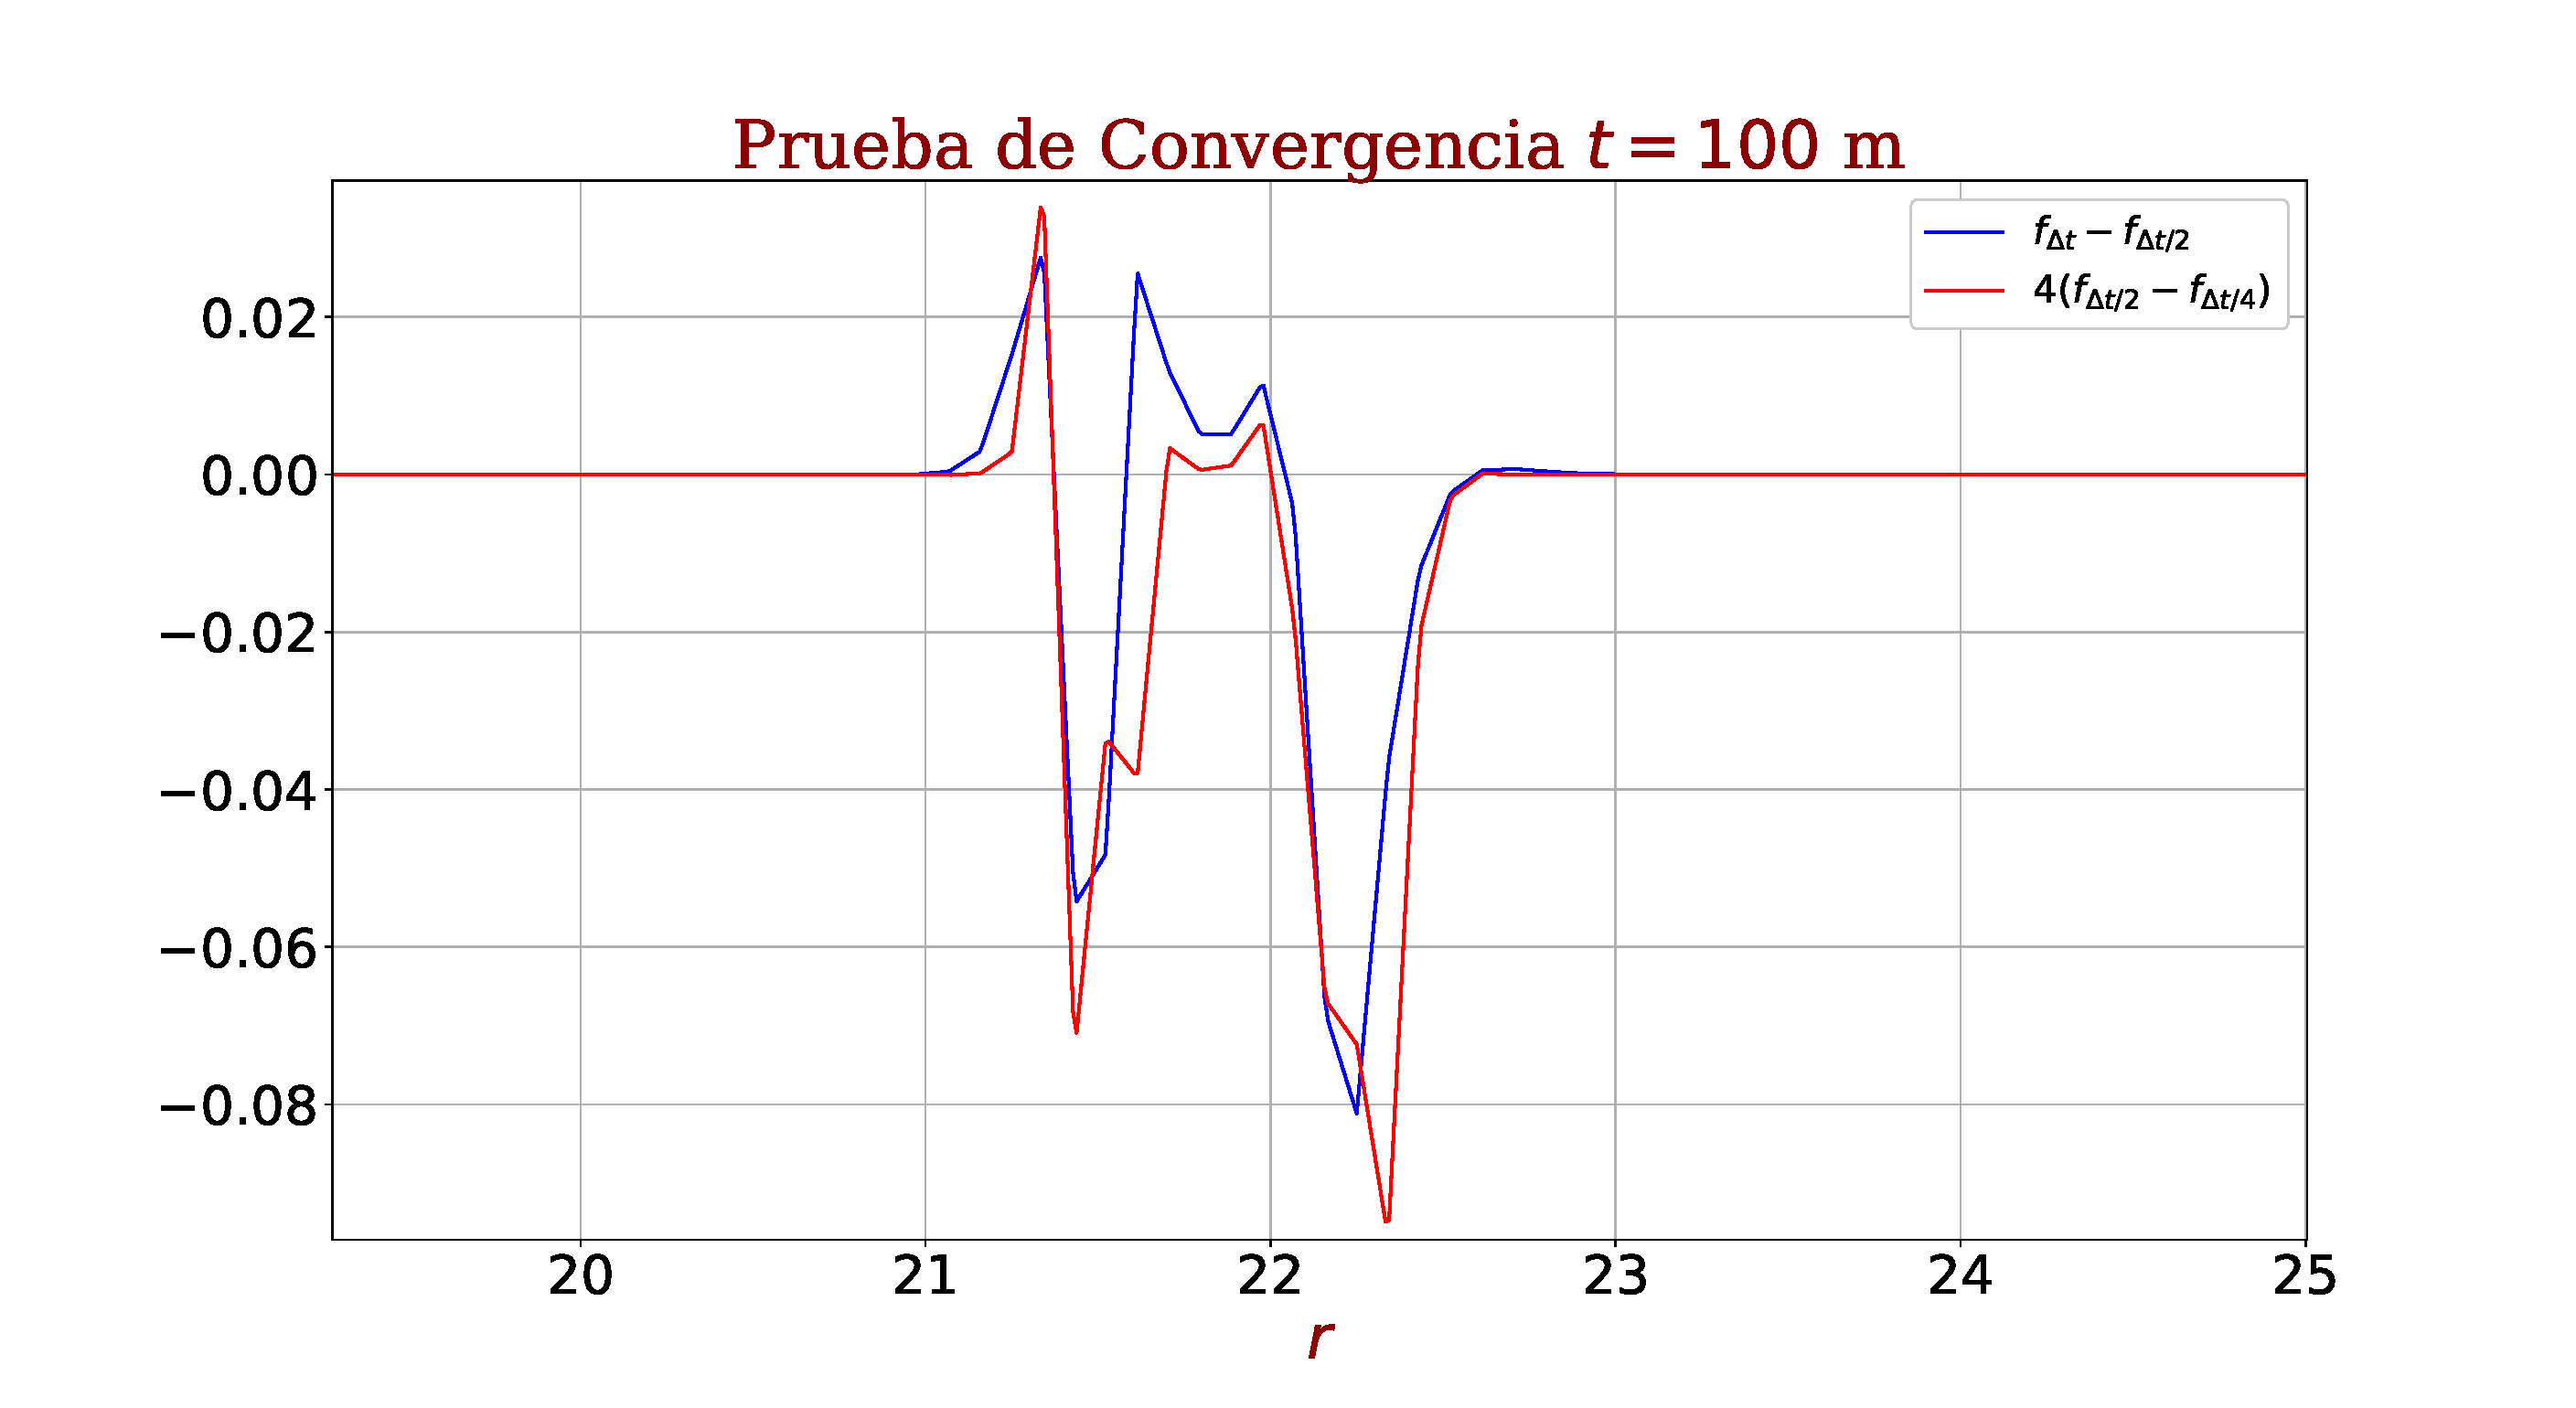
\includegraphics[width=0.8\textwidth]{graphs_study/LmayorKSGraphs/convergencetestKSMayor2}}
	\caption{Análisis de convergencia a diferentes tiempos de la evolución.}
	\label{convergenceksLmayor}
\end{figure}



\newpage
\begin{figure}[H]
	\centering
	\includegraphics[width=\textwidth,height=\textheight,keepaspectratio]{graphs_study/LmenorKSGraphs/evolutionKSMenor.png}
	\caption{Evolución de la función de distribución para $\tilde{L}=1.16\ M$ (es decir, $\tilde{L}<\sqrt{12}\ M$) en distintos tiempos en coordenadas de Kerr-Schild. Se observa que la función llega a la pared $r=M/4$ y pasa ese límite, sin embargo en este caso solo importa que logra pasar el horizonte de eventos. El color representa el valor de la función de distribución en cada punto.}
	\label{evolutionLmenorKS}
\end{figure}

\begin{figure}[H]
	\centering
	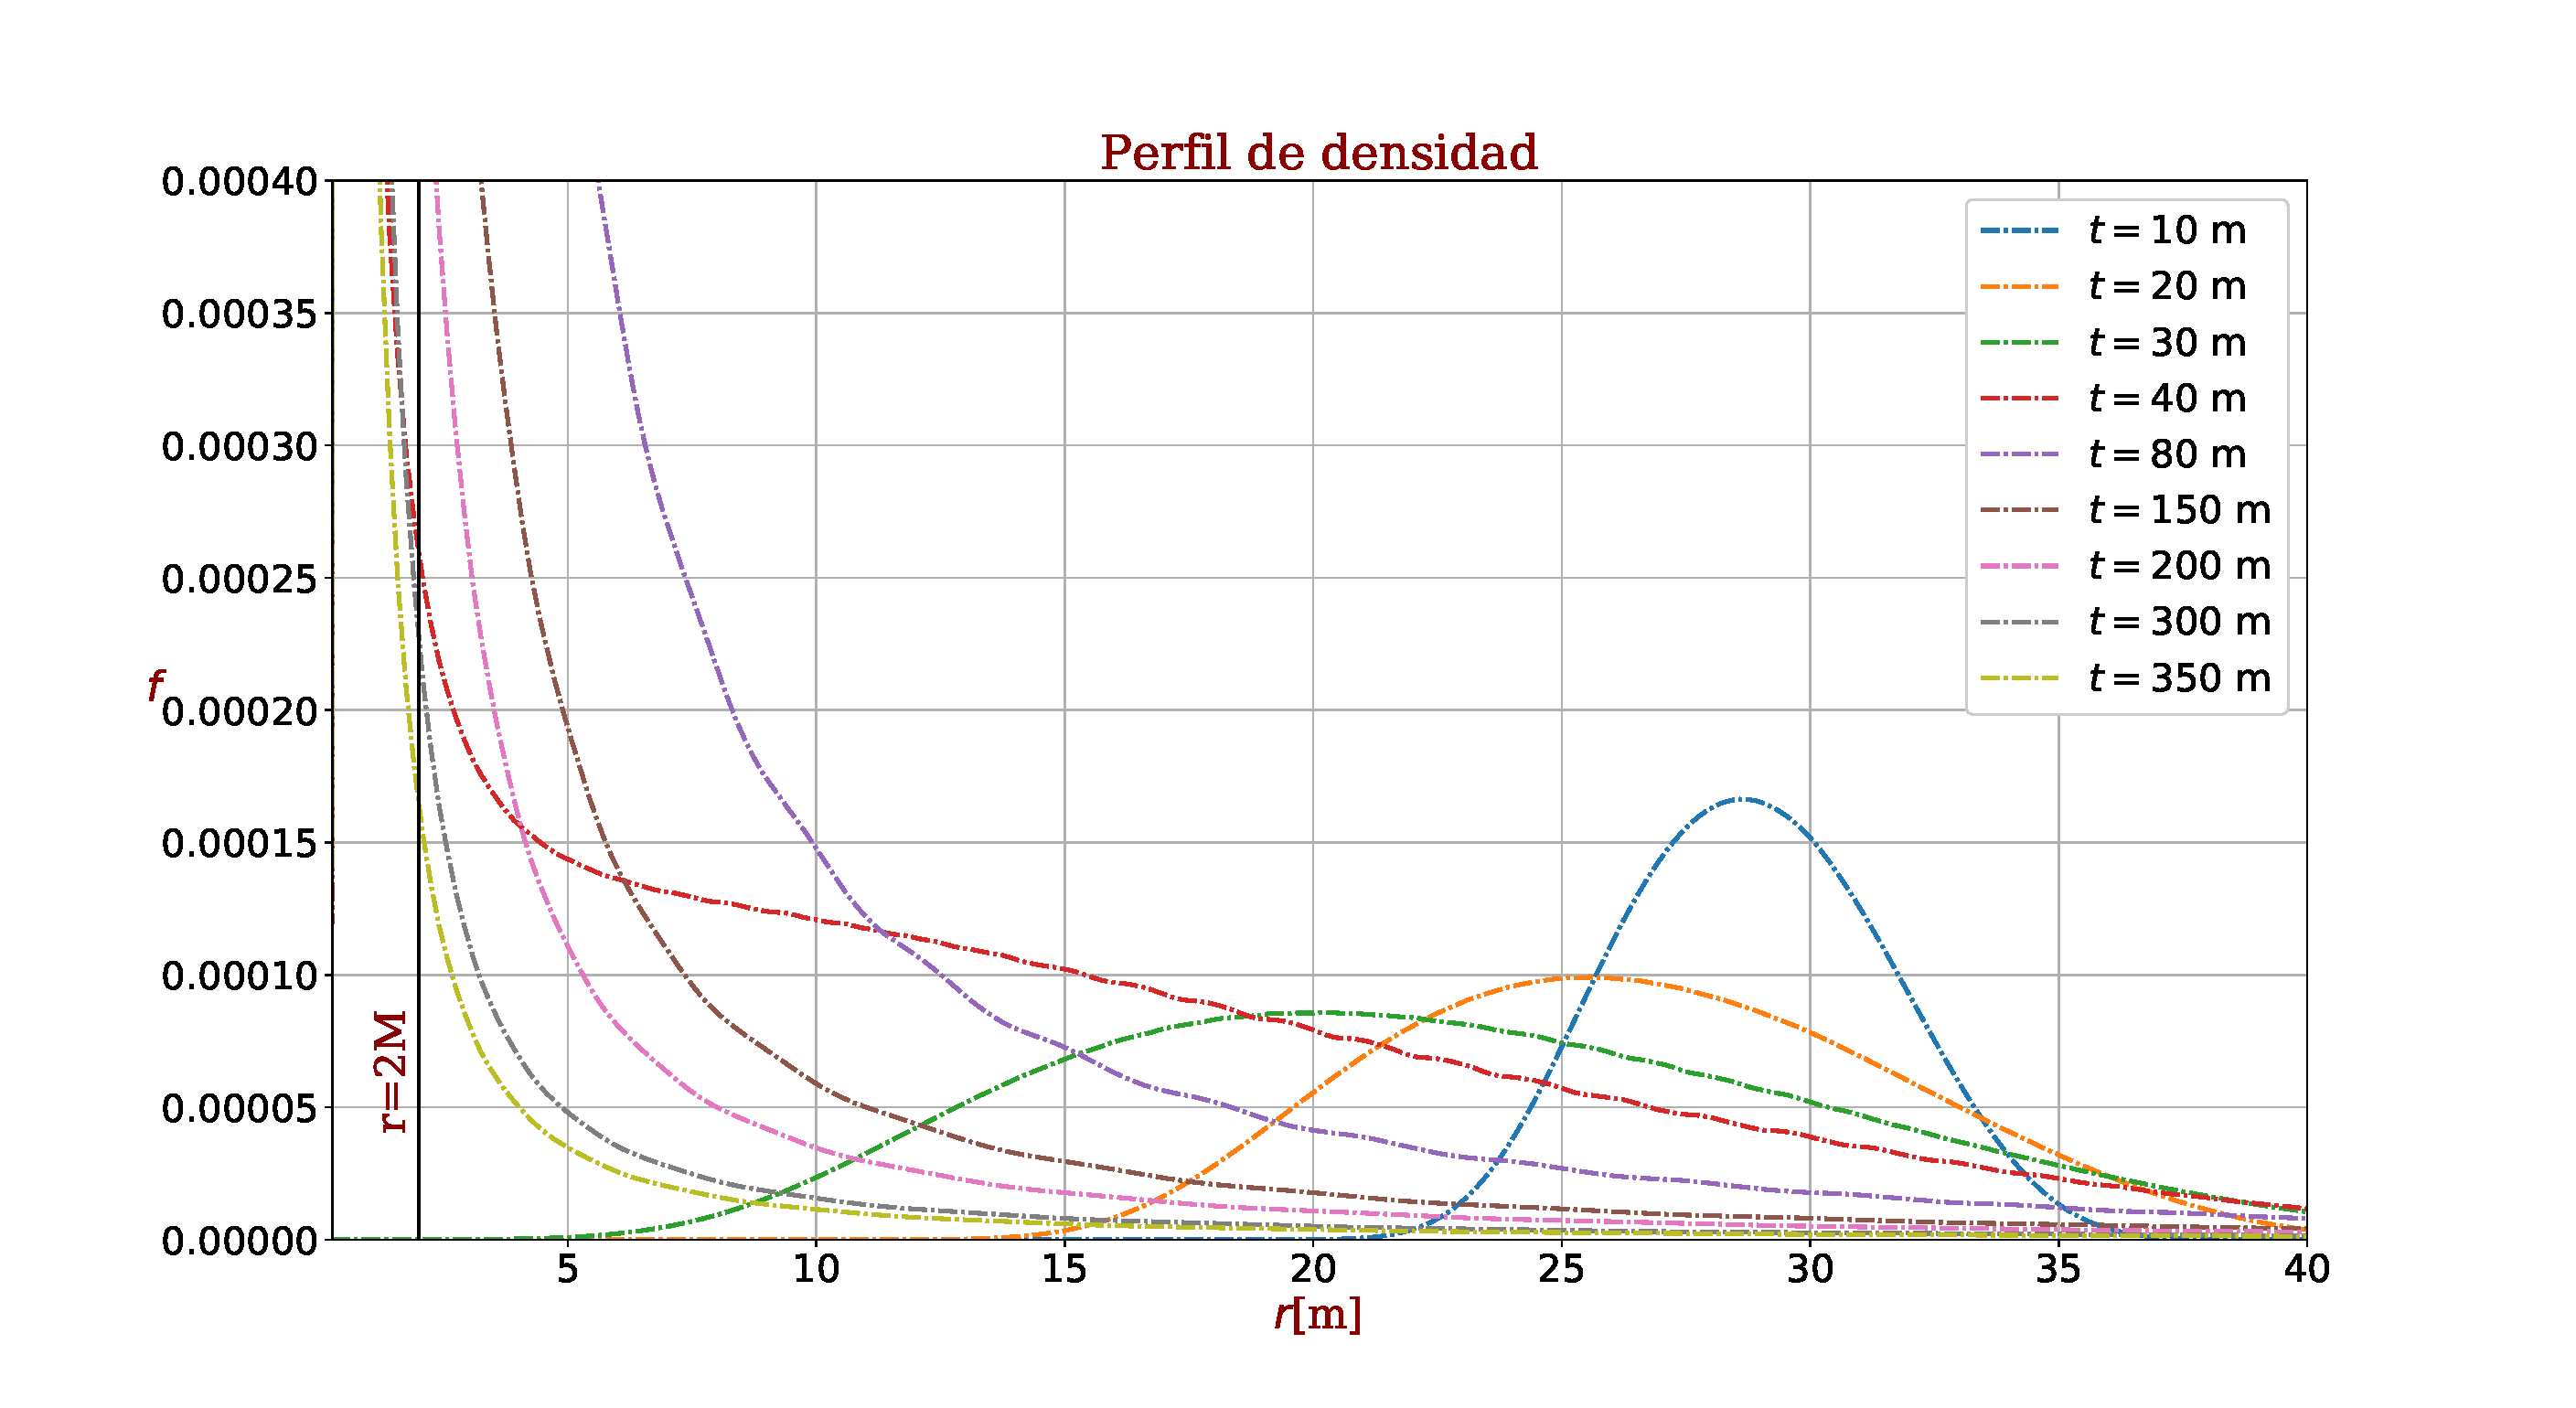
\includegraphics[height=8.75cm]{graphs_study/LmenorKSGraphs/densityProfileLmenorKS}
	\caption{Evolución del perfil de densidad de la función de distribución con $\tilde{L}=1.16\ M$, en coordenadas de Kerr-Schild. En estas gráficas se puede ver que en un principio, la función de distribución se incrementa su anchura y disminuye su amplitud. Después, se acerca al límite $r=M/4$ y comienza a entrar al agujero, es decir, pasa por el horizonte de eventos.}
	\label{densityProfileKSLmenor}
\end{figure}

\begin{figure}[H]
	\centering
	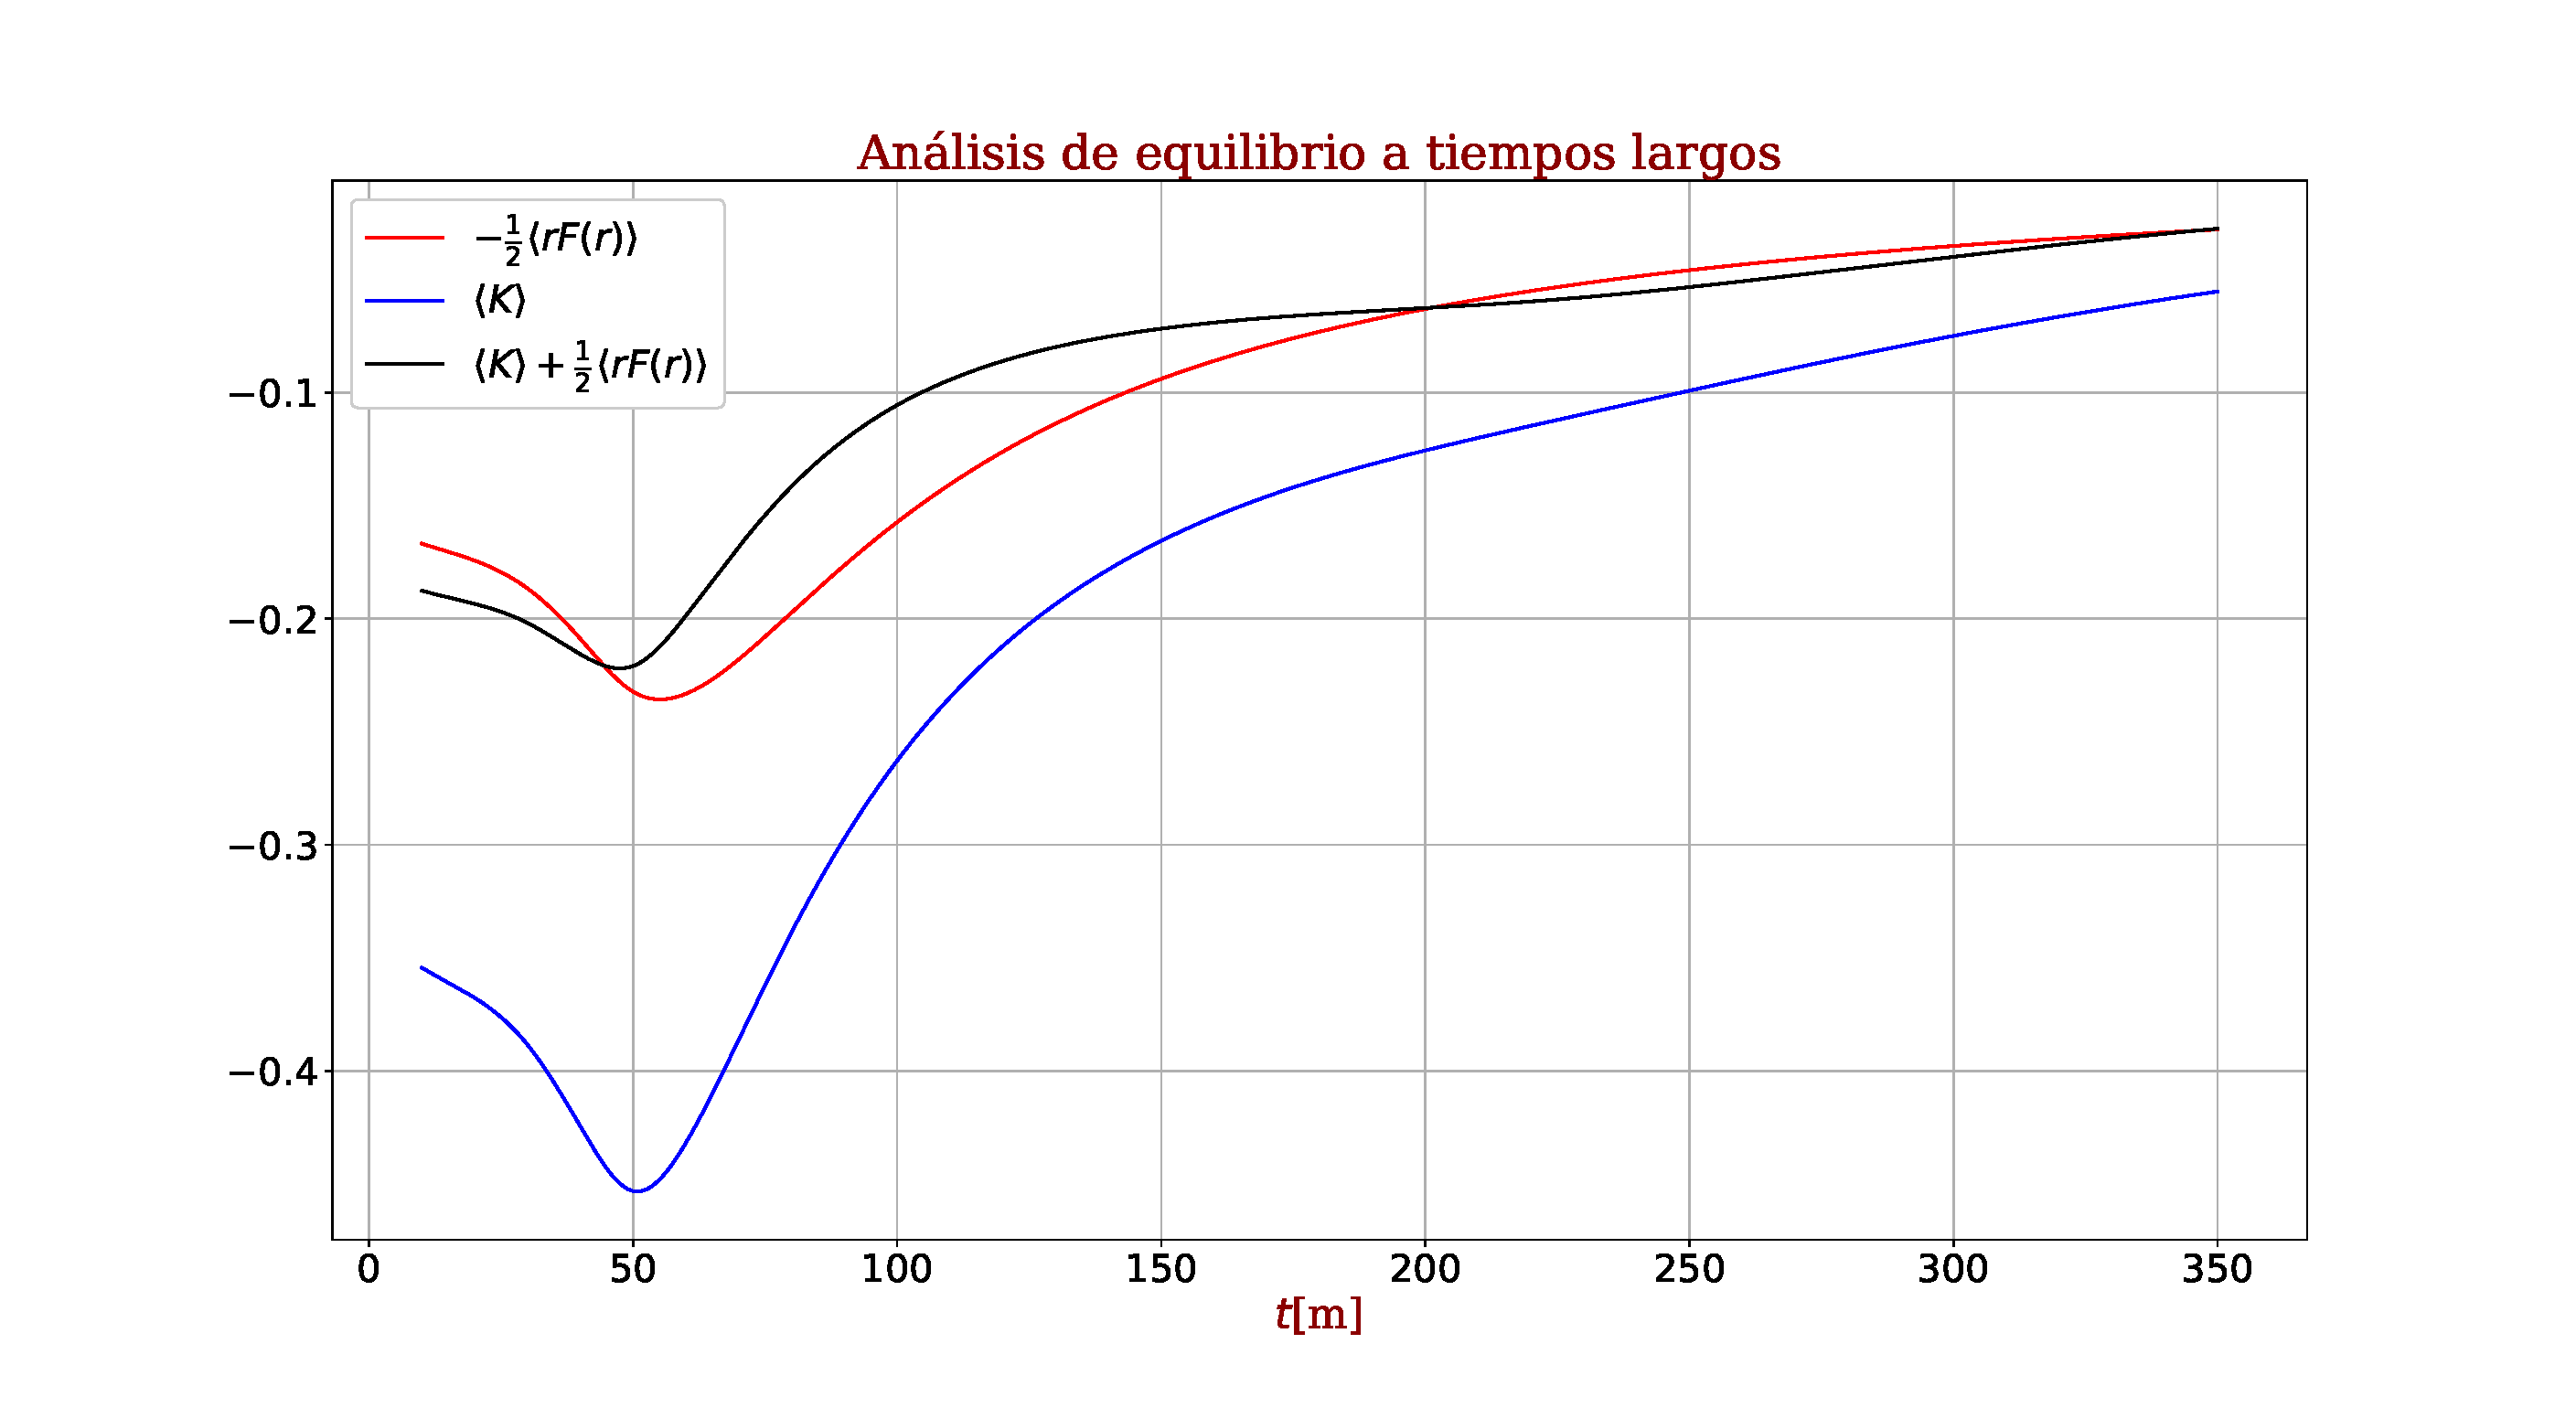
\includegraphics[height=8.75cm]{graphs_study/LmenorKSGraphs/stabilityKSMenor.eps}
	\caption{Análisis de equilibrio a tiempos largos. En la gráfica se muestra el promedio del virial $\frac{1}{2}\left<rF(r)\right>$ y de la energía cinética total $\left<K\right>$ para $\tilde{L}=1.16\ M$, en coordenadas de Kerr-Schild. En un estado estable, ambas gráficas deberían superponerse, lo cual no sucede nunca perfectamente. Sin embargo, la gráficas no se separan tanto. Esto es de esperarse, ya que las partículas no dejan de moverse y entrar más allá de $M/4$, por lo que nunca sucederá que dos gráficas sean totalmente iguales.}
	\label{stabilityKSLmenor}
\end{figure}

\begin{figure}[H]
	\centering
	\includegraphics[height=9cm]{graphs_study/LmenorKSGraphs/numpartKSMenor.eps}
	\caption{Evolución del número de partículas para $\tilde{L}=1.16\ M$, en coordenadas de Kerr-Schild. Al principio, la gráfica se mantiene constante. A un cierto tiempo algunas partículas comienzan a salir del dominio computacional en la frontera $r=M/4$ y no se detienen, por lo que nunca se llega realmente a un estado totalmente estable, como ya se mencionó.}
	\label{numpartKSMenor}
\end{figure}


\begin{figure}[H]
	\centering
	\subfloat[]{\label{}\includegraphics[width=0.8\textwidth]{graphs_study/LmenorKSGraphs/convergencetestKSMenor1}}	
	
	\subfloat[]{\label{}\includegraphics[width=0.8\textwidth]{graphs_study/LmenorKSGraphs/convergencetestKSMenor2}}
	
	\subfloat[]{\label{}\includegraphics[width=0.8\textwidth]{graphs_study/LmenorKSGraphs/convergencetestKSMenor3}}
	\caption{Análisis de convergencia a diferentes tiempos de la evolución.}
	\label{convergenceksLmenor}
\end{figure}

\chapter{Discusión y Conclusiones}
\noindent
En esta trabajo, se buscó un método numérico que permitiera el estudio estadístico de la ecuación de Vlasov relativista (EVR). Para ello, y gracias a que la estadística de un sistema se debe obtener mediante cuadraturas de la función de distribución, fue necesario encontrar métodos que preservaran la forma de dicha función sin presentar problemas de disipación ni de oscilaciones espurias. Dado que la EVR tiene la forma de una ecuación advectiva, se generalizaron los métodos usados para resolver este tipo de ecuaciones.

Partiendo de lo anterior, se encontró un problema: en la ecuación de advección de dos dimensiones \eqref{adv2d}, se presupone que las velocidades en cada dirección dependen de las coordenadas que definen estas direcciones y del tiempo (por ejemplo, $u_x=u_x(t,x)$), sin embargo, en la EVR, se observa que las velocidades en cada coordenada (en este caso, las coordenadas en el espacio-fase $r$ y $p_r$), dependen tanto de $r$ como de $p_r$ (ver ecuaciones \eqref{velr} y \eqref{velpr}). Sin embargo, se pudo demostrar que, aún con esto, la EVR toma la forma de una ley de conservación, por lo que se pudieron utilizar métodos conservadores de flujo y con esto, evitar dicho problema.

Precisamente en el anterior punto radica la diferencia que se puede encontrar entre los resultados obtenidos en este trabajo con otros estudios similares\footnote{Ver los artículos \citet{akbariancritical}, \citet{fujiwara1983} y \citet{Stevenson2003}, entre otros.} ya que aquí se supuso una métrica estacionaria cuyos términos no se veían afectados por las fuentes de masa descritas por el tensor de energía-momento, mismo que depende de la función de distribución $f$. Es necesario agregar esta dependencia en un estudio posterior para lograr resultados más acordes con un proceso físico. Para ello, se deben considerar las ecuaciones de constricción y de evolución que determinan ecuaciones diferenciales para los términos de la métrica. A continuación se describe brevemente lo anterior:

En las coordenadas de Schwarzschild\footnote{Dado que esto no es parte esencial del trabajo, no se hará el tratamiento en coordenadas de Kerr-Schild, sólo se realiza para dar una idea de lo que sería un estudio posterior.}, es sencillo ver que la constricción Hamiltoniana descrita en simetría esférica por la ecuación \eqref{consthamiltonianaesferica} toma la forma 
\begin{equation}
\partial_r A=\frac{A}{r}\left(1-A\right)-8\pi A^2r\tensor{S}{^t_t}
\label{ecuacionA}
\end{equation}
donde se usó que $K=\tensor{K}{^i_i}=\tensor{K}{^r_r}$. Esto último, junto con la condición de $\beta_r=0$ y $B=1$ de manera que el área propia de las esferas con $r$ constante es siempre $4\pi r^2$, se conoce como \textit{polar-areal gauge}\footnote{Ver \citet{alcubierre}, p. 371.}. Asimismo, de la ecuación de evolución ADM para $K_B$ \eqref{cambiokb}, y usando \eqref{ecuacionA}, se obtiene
\begin{equation}
\partial_r \alpha=\frac{\alpha}{2r}\left(A-1\right)+\frac{rA\alpha}{2}8\pi \tensor{S}{^r_r}
\label{ecuacionalpha}
\end{equation}
Los dos términos del tensor de energía momento que se observan en las ecuaciones anteriores se pueden obtener de la ecuación \eqref{tensenergmomentof}, de donde:
\begin{eqnarray}
\tensor{S}{^t_t}=-\frac{\pi\alpha}{Ar^2}\int p^0 f(t,r,p_r,l^2)\ \text{d}p_r\ \text{d}L^2\\
\tensor{S}{^r_r}=\frac{\pi}{Ar^2\alpha}\int p_rf(t,r,p_r,l^2)\ \text{d}p_r\ \text{d}L^2
\end{eqnarray}

Las ecuaciones \eqref{ecuacionA} y \eqref{ecuacionalpha} se deben resolver para obtener $A$ y $\alpha$ a cada tiempo y así poder utilizarlas en la ecuación de Vlasov, y dado que el tensor de energía-momento depende tanto de $A$ como de $\alpha$, se concluye que son dos ecuaciones diferenciales de primer orden acopladas. Para resolver la ecuación \eqref{ecuacionA} se deben de satisfacer dos tipos de condiciones en $r=0$, la primera de ellas es aquella impuesta por el requerimiento de que las variables estén bien definidas en el origen, de manera que 
\begin{equation}
A\sim A^0+\mathcal{O}\{r^2\}, \hspace{2cm}B\sim B^0+\mathcal{O}\{r^2\}
\end{equation}
con $A^0$ y $B^0$ funciones del tiempo en general. Para implementar esta condición numéricamente, se debe utilizar una malla movida en el origen de manera que se obtengan datos en la frontera en un punto ficticio $r=-\Delta r/2$ pidiendo que $A$ sea una función par en $r=0$. La otra condición es una consecuencia de que el espacio debe permanecer localmente plano cerca del origen $r=0$, o en otras palabras, dada la constricción Hamiltoniana \eqref{ecuacionA}, para evitar términos que van como $1/r^2$, se debe tener
\begin{equation}
A-B\sim\mathcal{O}\{r^2\}
\end{equation}
lo que implica $A^0=B^0$, y por la condición de \textit{polar-areal gauge}, entonces $A^0=1$. De esta manera se tiene que en el origen, la condición que debe implementarse es $A(r=0)=1$. Después de obtener $A(t,r)$ para un tiempo, se puede substituir en \eqref{ecuacionalpha} para obtener $\alpha(t,r)$ para dicho tiempo, la forma de hacerlo es integrando hacia adentro desde $r=r_{\text{max}}$ con la condición 
\begin{equation}
\alpha(r_{\text{max}})=\frac{1}{\sqrt{A(r_{\text{max}})}}
\end{equation}

Una vez hecho lo anterior, se concluye que tanto $\alpha$ como $A$ dependen del tiempo, la posición y el momento, por lo que entonces las velocidades en $r$ y $p$ ($\text{d}r/\text{d}t$ y $\text{d}p/\text{d}t$ respectivamente) no solo dependerán de la posición y el momento en un caso más general, sino también del tiempo, por lo que las fórmulas en diferencias finitas deberán ser modificadas para tener en cuenta está característica\footnote{Ver \citet{schullenfdmfaivvf} y \citet{Thomas1998} para ejemplos de cómo generalizar una fórmula en diferencias finitas, es decir, hacerlas de un orden mayor y que además permitan incluir las dependencias de la velocidad en la posición y el tiempo.}.

Asimismo y como ya se comentó, fue necesario utilizar una aproximación clásica del Teorema del Virial para realizar los análisis de equilibrio a tiempos largos. Debido a la falta de un teorema para el caso relativista en el caso de un espacio-tiempo estático de fondo (análogo al caso de un potencial externo Newtoniano), sería conveniente buscar esta generalización en un futuro debido a la utilidad de dicho teorema.

Finalmente, es necesario que este estudio sea también generalizado al caso en que las partículas posean distintos momentos angulares, aún cuando esto involucre un mayor problema computacional al considerar un espacio-fase tres dimensional. Además, este trabajo pretende actuar como una base en el estudio de la materia obscura desde el punto de vista de la teoría cinética relativista, permitiendo un acercamiento mucho más sencillo al que proporcionan las simulaciones de N-cuerpos\footnote{Ver \citet{Colombi2015}.}. Es posible, por ejemplo, buscar potenciales gravitacionales que representen distintos modelos de halos de materia obscura, mientras que la función de distribución puede representar una inhomogeneidad de materia oscura dentro de dicho halo\footnote{Ver \citet{Dominguez2017}.}.

%------------------------------------------------------------------------------------------ %
\clearpage
\appendix 

\fancyhead[LE]{\scshape\thepage\hspace{1cm}\footnotesize\nouppercase{Apéndices}}
\fancyhead[RO]{\scshape\footnotesize\nouppercase{Apéndice \thechapter}\hspace{1cm}\normalsize\thepage}
\fancyhead[LO]{}
\fancyhead[RE]{}
\pagestyle{fancy}

\chapter{Constricciones en simetría esférica}\label{desarrolloconstadm}
La parte puramente espacial de la métrica en simetría esférica en el formalismo 3+1 es
\begin{equation}
dl^2=A\ dr^2+Br^2\left(d\theta^2+\sin^2\theta\ d\phi^2\right)
\end{equation}

Se observa que la constricción hamiltoniana \eqref{constriccionhamiltoniana} involucra el escalar de curvatura $R$ asociado a la métrica. Para encontrarlo basta con usar un programa de cálculo simbólico (en este caso se usa Maple 2016), con lo que se obtiene 
\begin{equation*}
R = -\frac{2}{A}\frac{\partial_r^2B}{B}+\frac{1}{2A}\frac{(\partial_r B)^2}{B^2}+\frac{1}{A^2}\frac{\partial_rB}{B}\frac{\partial_r A}{A}-\frac{6}{r}\frac{\partial_r B}{BA}+\frac{2}{rA}\frac{\partial_rA}{A}+\frac{2}{r^2B}-\frac{2}{r^2A}
\end{equation*}
Definiendo $K_A\coloneqq K_r^r$, $K_B\coloneqq K_{\theta}^{\theta}=K_{\phi}^\phi$, $D_A\coloneqq\partial_r\ln A$ y  $D_B\coloneqq\partial_r \ln B$, se puede escribir explícitamente el término que involucra la curvatura extrínseca de la siguiente manera
\begin{equation*}
K^2-K_{ij}K^{ij}=(2K_B+K_A)^2-\gamma_{ip}\gamma^{im}K_j^pK^j_m=\delta^m_p K_j^pK_m^j=K_j^mK^j_m
\end{equation*}
y usando que $K_i^j$ tiene solo componentes en la diagonal, entonces $K_j^mK^j_m=K_r^rK_r^r+K_\theta^\theta K_\theta^\theta+K_\phi^\phi K_\phi^\phi$, por lo tanto
\begin{align*}
K^2-K_{ij}K^{ij}&=(2K_B+K_A)^2-K_A^2-2K_B^2=4K_B^2+K_A^2+4K_BK_A-K_A^2-2K_B^2=2K_B^2+4K_BK_A\\
&=K_B(2K_B+4K_A)
\end{align*}
de tal forma, la ecuación \eqref{constriccionhamiltoniana} se reescribe
\begin{align*}
\frac{\partial_r^2B}{B}-\frac{\left(\partial_rB\right)^2}{B^2}=-\frac{3}{4}\frac{\left(\partial_rB\right)^2}{B^2}+\frac{1}{2}\frac{\partial_rB}{B}\frac{\partial_rA}{A}-\frac{3}{r}\frac{\partial_rB}{B}+\frac{1}{r}\frac{\partial_rA}{A}+\frac{A}{r^2B}-\frac{1}{r^2}+\frac{A}{2}\ K_B\ (2K_B+4K_A)-8\pi\rho A
\end{align*}
Donde podemos expresar la parte de la izquierda de la anterior ecuación como
\begin{align*}
\frac{\partial_r^2B}{B}-\frac{\left(\partial_rB\right)^2}{B^2}=\partial_r\left( \frac{\partial_rB}{B}\right)=\partial_r D_B
\end{align*}
para obtener una expresión de la constricción hamiltoniana para la métrica dada por \eqref{metricaesfericaespacial}
\begin{equation}
\partial_r D_B=-\frac{3D_B^2}{4}+\frac{D_A D_B}{2}+\frac{1}{r}\left(D_A-3D_B\right)+\frac{1}{r^2B}\left(A-B\right)+AK_B\left(2K_A+K_B\right)-8\pi A\rho
\end{equation}
Partiendo ahora de la constricción de momento
\begin{align*}
D_j\left(K^{ij}-\gamma^{ij}K^m_m\right)=8\pi S^i\Rightarrow \gamma_{il}D_j\left(K^{ij}-\gamma^{ij}K^m_m\right)=8\pi S^i\gamma_{il}\\
D_j\left(\gamma_{il}K^{ij}-\gamma_{il}\gamma^{ij}K^m_m\right)-\left(K^{ij}-\gamma^{ij}K^m_m\right)D_j\gamma_{il}=8\pi S_l\\
D_j\left(K^j_l-\delta^j_l K_m^m\right)-K^{ij}D_j\gamma_{il}+\gamma^{ij}K_m^m D_j\gamma_{il}=8\pi S_l\\
D_jK^j_l-D_l K_m^m-\gamma^{ip}K^j_p D_j\gamma_{il}+\gamma^{ij}K_m^m D_j\gamma_{il}=8\pi S_l
\end{align*}
y sabiendo que 
\begin{align*}
D_b B^m_n=\partial_b B^m_n+B^a_n\ ^{(3)}\Gamma^m_{ab}-B^m_a\ ^{(3)}\Gamma^a_{nb}\\
D_b T_{mn}=\partial_b T_{mn}-T_{an}\ ^{(3)}\Gamma^a_{mb}-T_{ma\ ^{(3)}}\Gamma^a_{nb}
\end{align*}
siendo $^{(3)}\Gamma^g_{bm}$ los símbolos de Cristoffel asociados a la métrica espacial
\begin{equation*}
^{(3)}\Gamma^g_{bm}=\frac{1}{2}\gamma^{ag}\left(\partial_m \gamma_{ab}+\partial_b \gamma_{am}-\partial_a \gamma_{bm}\right)
\end{equation*}
se tiene entonces que
\begin{align*}
\partial_j K^j_l + K^a_l\ ^{(3)}\Gamma^j_{aj}-K^j_a\ ^{(3)}\Gamma^a_{lj}-\partial_l K^m_m- K^p_m\ ^{(3)}\Gamma^m_{pl}+K^m_a\ ^{(3)}\Gamma^a_{ml}-\gamma^{ip}K^j_p D_j\gamma_{il}+\gamma^{ij}K_m^m D_j\gamma_{il}=8\pi S_l
\end{align*}
Usando la simetría de los Christoffel obtenemos 
\begin{align*}
\partial_l K^m_m=\partial_j K^j_l + K^a_l\ ^{(3)}\Gamma^j_{aj}- K^p_m\ ^{(3)}\Gamma^m_{pl}+\left(\gamma^{ij}K_m^m -\gamma^{ip}K^j_p\right)D_j\gamma_{il}-8\pi S_l
\end{align*}
Así, podemos hacer las operaciones respectivas
\begin{align*}
\partial_r (K^r_r+K_\theta^\theta+K_\phi^\phi)=\partial_r K^r_r + K^r_r\ ^{(3)}\Gamma^j_{rj}- K^p_m\ ^{(3)}\Gamma^m_{pr}+\left(\gamma^{rr}K_m^m -\gamma^{rr}K^r_r\right)D_r\gamma_{rr}-8\pi S_r
\end{align*}
donde se usó que solo los componentes $K_r^r, K^\theta_\theta, K_\phi^\phi$ son distintos de cero, y que solo la diagonal tanto de la métrica como de su inversa son distintas de cero. Usando las definiciones dadas anteriormente, esta expresión se reduce a
\begin{align}
\nonumber
2\partial_r K_B&=K^r_r\ ^{(3)}\Gamma^r_{rr}+K^r_r\ ^{(3)}\Gamma^\theta_{r\theta}+K^r_r\ ^{(3)}\Gamma^\phi_{r\phi}- K^r_r\ ^{(3)}\Gamma^r_{rr}-K^\theta_\theta\ ^{(3)}\Gamma^\theta_{\theta r}-K^\phi_\phi\ ^{(3)}\Gamma^\phi_{\phi r}\\
\nonumber
&+\left(\gamma^{rr}K_m^m -\gamma^{rr}K^r_r\right)\left(\partial_r \gamma_{rr}-\gamma_{rr}\ ^{(3)}\Gamma^r_{rr}-\gamma_{rr}\ ^{(3)}\Gamma^r_{rr}\right)-8\pi S_r\\
\nonumber
&=K^r_r\ ^{(3)}\Gamma^\theta_{r\theta}+K^r_r\ ^{(3)}\Gamma^\phi_{r\phi}-K^\theta_\theta\ ^{(3)}\Gamma^\theta_{\theta r}-K^\phi_\phi\ ^{(3)}\Gamma^\phi_{\phi r}\\
&+\left(\gamma^{rr}K_m^m -\gamma^{rr}K^r_r\right)\left(\partial_r \gamma_{rr}-2\gamma_{rr}\ ^{(3)}\Gamma^r_{rr}\right)-8\pi S_r
\label{constmomento1}
\end{align}
Calculamos los Christoffel que aparecen en la expresión anterior
\begin{align*}
\ ^{(3)}\Gamma^\theta_{r\theta}&=\frac{1}{2}\gamma^{\theta\theta}\left(\partial_r\gamma_{\theta\theta}+\partial_\theta\gamma_{\theta r}-\partial_\theta \gamma_{r\theta}\right)=\frac{1}{2r^2B}\left(2rB+r^2\partial_rB\right)\\
\ ^{(3)}\Gamma^\phi_{r\phi}&=\frac{1}{2}\gamma^{\phi\phi}\left(\partial_r\gamma_{\phi\phi}+\partial_\phi\gamma_{\phi r}-\partial_\phi \gamma_{r\phi}\right)=\frac{1}{2r^2B\sin^2\theta}\left(2rB\sin^2\theta+r^2\partial_rB\sin^2\theta\right)=\ ^{(3)}\Gamma^\theta_{r\theta}\\
\ ^{(3)}\Gamma^r_{rr}&=\frac{1}{2}\gamma^{rr}\left(\partial_r\gamma_{rr}+\partial_r\gamma_{r r}-\partial_r\ ^{(3)}\gamma_{rr}\right)=\frac{1}{2A}\partial_r A\\
\end{align*}
y substituyendo en \eqref{constmomento1}
\begin{align*}
2\partial_r K_B&=\left(2K_A-2K_B\right)\left[\frac{1}{2r^2B}\left(2rB+r^2\partial_rB\right)\right]+\left(\gamma^{rr}K_m^m -\gamma^{rr}K^r_r\right)\left(\partial_rA-2A\frac{1}{2A}\partial_r A\right)-8\pi S_r\\
&=\left(2K_A-2K_B\right)\left[\frac{1}{r}+\frac{\partial_rB}{2B}\right]-8\pi S_r=\left(2K_A-2K_B\right)\left[\frac{1}{r}+\frac{\partial_r\ln B}{2}\right]-8\pi S_r
\end{align*}
Finalmente, la constricción de momento para la métrica dada por \eqref{metricaesfericaespacial} se reduce a 
\begin{equation}
\partial_r K_B=\left(K_A-K_B\right)\left[\frac{1}{r}+\frac{D_B}{2}\right]-4\pi S_r
\end{equation}

\chapter{Geometría y Topología Diferencial}\label{gytd}

\noindent
En esta sección se encuentran las formas de volumen necesarias para derivar la ecuación de Vlasov en Relatividad General. Este apéndice se basa enteramente en el artículo \citet{debbasch1} y en los libros \citet{boothbyaitdmarg} y \citet{spivakcm}.

\section{Formas de Volumen}
Una uno-forma es un campo sobre el haz tangente $\mathcal{TM}$ de una variedad que actúa de manera lineal sobre campos vectoriales de la variedad $\mathcal{M}$. El espacio de las uno-formas sobre $\mathcal{M}$ se denota como $\mathcal{T^*M}$ o como $\Omega^1(M)$. Dada una base $e_\alpha$ de $\mathcal{TM}$, su base dual se denota como el conjunto de uno-formas $e^\alpha$ que cumplen $e^\alpha\left(e_\beta\right)=\delta^\alpha_\beta$.  En el caso particular que toma a $\partial_\alpha$ como la base de $\mathcal{TM}$, su base dual es $\text{d}x^\alpha$.

Se denota el espacio de las p-formas como $\Omega^p(M)$, una p-forma sobre una carta dada es una combinación lineal de productos de la base dual $\text{d}x^\alpha$
\begin{equation}
\omega=\frac{1}{p!}\omega_{\alpha_1 \alpha_2\dots\alpha_p}\ \text{d}x^{\alpha_1}\wedge\text{d}x^{\alpha_2}\wedge\dots\wedge\text{d}x^{\alpha_p}
\end{equation}
donde $\wedge$ denota al producto exterior. Esta p-forma se puede integrar sobre una subvariedad $\Omega$ de $\mathcal{M}$ para obtener
\begin{equation}
\int_\Omega \omega=\int_{\Omega}\frac{1}{p!}\omega_{\alpha_1 \alpha_2\dots\alpha_p}\ \text{d}x^{\alpha_1}\wedge\text{d}x^{\alpha_2}\wedge\dots\wedge\text{d}x^{\alpha_p}
\end{equation}
entendiendo a $\text{d}x^\alpha$ como diferenciales para la integración. Un caso particular es el de una variedad pseudoriemanniana, misma en la que se puede definir una forma de volumen por medio de la elección de la siguiente p-forma
\begin{equation}
\text{d}^pV\coloneqq\frac{1}{p!}\sqrt{-g}\epsilon_{\alpha_1 \alpha_2\dots\alpha_p}\text{d}x^{\alpha_1}\wedge\text{d}x^{\alpha_2}\wedge\dots\wedge\text{d}x^{\alpha_p}
\end{equation} 
donde $\epsilon_{\alpha_1 \alpha_2\dots\alpha_p}$ es el símbolo de permutación de Levi-Civita que cambia su valor en función de las permutaciones de $\left\{\alpha_1 \alpha_2\dots\alpha_p\right\}$ respecto a $\left\{0,1,\dots,p-1\right\}$ (donde $\alpha_j$ denotan las coordenadas utilizadas), de la siguiente manera 
\begin{equation}
\epsilon_{\alpha_1 \alpha_2\dots\alpha_p} = \left\{
\begin{array}{ll}
+1      & \text{Permutación par de }\left\{0,1,\dots,p-1\right\}\\
-1      & \text{Permutación impar de }\left\{0,1,\dots,p-1\right\}\\
0       & \text{Cualquier otra forma}
\end{array}
\right.
\end{equation}
La definición de elementos de volumen $p-k$ dimensionales toma la siguiente forma general
\begin{equation}
\text{d}^{p-k}V_{\alpha_1\alpha_2\dots\alpha_k}=\frac{1}{\left(p-k\right)!}\sqrt{-g}\epsilon_{\alpha_1\alpha_2\dots\alpha_k\beta_1\beta_2\dots\beta_{p-k}}\ \text{d}x^{\beta_1}\wedge\text{d}x^{\beta_2}\wedge\dots\wedge\text{d}x^{\beta_{p-k}}
\end{equation}
siendo que lo mismo debe suceder si se integra sobre las componentes covariantes
\begin{equation}
\text{d}^{p-k}V_{*}^{\alpha_1\alpha_2\dots\alpha_k}=\frac{1}{\left(p-k\right)!}\frac{1}{\sqrt{-g}}\epsilon^{\alpha_1\alpha_2\dots\alpha_k\beta_1\beta_2\dots\beta_{p-k}}\ \text{d}x_{\beta_1}\wedge\text{d}x_{\beta_2}\wedge\dots\wedge\text{d}x_{\beta_{p-k}}
\label{elvolcov}
\end{equation}
notando que la métrica en el espacio dual $\mathcal{T^*M}$ es el inverso de $g_{\alpha\beta}$ y que el símbolo de permutación con índices arriba tiene la misma definición que con índices abajo. 

De esta manera, se define un \textbf{elemento de superficie tridimensional en una hoja $\Sigma(t)$ de una foliación} como
\begin{equation}
\text{d}^3\Sigma_\mu\coloneqq \frac{1}{3!}\sqrt{-g}\ \epsilon_{\mu\nu\rho\sigma}\ \text{d}x^\nu\wedge\text{d}x^\rho\wedge\text{d}x^\sigma
\end{equation}
En un sistema de coordenadas adaptadas a la foliación, $\text{d}x^0=0$, por lo que para un tensor arbitrario $T(x,p)$ se tiene
\begin{equation}
\int_{V_x}T(x,p)\ \text{d}^3\Sigma_\mu=\int_{V_x} T(x,p)\frac{1}{3!}\ \sqrt{-g}\ \epsilon_{\mu ijk}\ \text{d}x^i\wedge\text{d}x^j\wedge\text{d}x^k
\end{equation}
y como $\epsilon_{\mu ijk}=\delta^0_\mu\epsilon_{ijk}$ entonces
\begin{equation}
\int_{V_x}T(x,p)\ \text{d}^3\Sigma_\mu=\delta^0_\mu\int_{V_x} T(x,p)\frac{1}{3!}\ \sqrt{-g}\ \epsilon_{ijk}\ \text{d}x^i\wedge\text{d}x^j\wedge\text{d}x^k
\end{equation}
por lo tanto, en dicho sistema de coordenadas, se obtiene que
\begin{equation}
\text{d}^3\Sigma_\mu=\delta^0_\mu\sqrt{-g}\ \text{d}^3x\label{dsigma}
\end{equation}
donde 
\begin{equation}
\text{d}^3x=\frac{1}{3!}\ \epsilon_{ijk}\ \text{d}x^i\wedge\text{d}x^j\wedge\text{d}x^k
\end{equation}

Restringiendo el estudio a la capa de masa, y considerando que $p_\mu p^\mu=-m^2$ lleva a
\begin{align}
p_\mu\frac{\text{d}p^\mu}{\text{d}p^j}=0\hspace{0.3cm}\Rightarrow\hspace{0.3cm}p_0\frac{\text{d}p^0}{\text{d}p^j}+p_k\delta^k_j=0\hspace{0.3cm}\Rightarrow\hspace{0.3cm} \text{d}p^0=\frac{-p_k}{p_0}\ \text{d}p^k
\end{align} 
es posible obtener la \textbf{forma de volumen en la capa de masa} tomando la norma de la 3-forma de volumen del espacio de momentos
\begin{equation}
\text{d}^3V_{p_*}=\sqrt{\text{d}V_*^\alpha\ \text{d}V_{*\alpha}}
\end{equation}
donde, usando la relación \eqref{elvolcov}, se tiene
\begin{equation}
\text{d}^3V_*^\alpha=\frac{1}{\sqrt{-g}}\frac{p^\alpha}{p^0}\ \text{d}^3p_*\hspace{0.3cm}\Rightarrow\hspace{0.3cm}\text{d}^3V_{p_*}=\frac{1}{\sqrt{-g}}\frac{m}{p^0}\ \text{d}^3p_*
\label{volelempa}
\end{equation}
De una forma análoga y partiendo de \eqref{dsigma}, se llega a la expresión para la forma de volumen en el espacio de posiciones
\begin{equation}
d^3V_x=\frac{p^0}{m}\sqrt{-g}\ \text{d}^3x
\label{volelemxa}
\end{equation}

\newpage

\begin{comment}
\section{Teorema de Stokes}\label{ts}
\noindent
El Teorema de Stokes es un resultado fundamental que tiene que ver con la integración de formas en variedades \citet{andrewslodg}. El teorema dice lo siguiente: Sea $M^{n+1}$ una variedad diferenciable compacta con frontera, y sea $\omega\in\Omega^{n}(M)$, entonces
\begin{equation}
\int_M \text{d}\omega=\int_{\partial M} \omega
\end{equation}
donde $\partial\Omega$ denota la frontera de $\Omega$, y $\text{d}$ es el operador de derivada exterior \citet[pág. 133]{andrewslodg}, donde dicho operador es un mapeo único entre formas diferenciales $\text{d}:\Omega^{n}(M)\rightarrow\Omega^{n+1}(M)$ y cumple lo siguiente

\begin{itemize}
	\item Si $f\in \Omega^0(M)=C^\infty(M)$, entonces $\text{d} f$ es la diferencial de $f$
	\item Si $\omega\in\Omega^k(M)$ y $\eta\in\Omega^p(M)$ entonces
	\begin{equation*}
	\text{d}\left(\omega\wedge\eta\right)=\left(\text{d}\omega\right)\wedge\eta+\left(-1\right)^k\omega\wedge\left(\text{d}\eta\right)
	\end{equation*}
	\item $\text{d}^2=0$
\end{itemize}

En coordenadas locales, la derivada exterior de una p-forma se escribe como
\begin{align}
\omega&=\frac{1}{p!}\omega_{\alpha_1 \alpha_2\dots\alpha_p}\ \text{d}x^{\alpha_1}\wedge\text{d}x^{\alpha_2}\wedge\dots\wedge\text{d}x^{\alpha_p}\\
\Rightarrow\hspace{0.3cm}\text{d}\omega&=\frac{1}{\left(p+1\right)!}\ \partial_\beta\omega_{\alpha_1\alpha_2\dots\alpha_p}\ \text{d}x^\beta\wedge\text{d}x^{\alpha_1}\wedge\text{d}x^{\alpha_2}\wedge\dots\wedge\text{d}x^{\alpha_p}
\end{align}
Como un ejemplo, se considera una 2-forma espacial
\begin{align}
\omega&=\frac{1}{2!}\epsilon_{ijk}\ \upsilon^i\ \text{d}x^j\wedge\text{d}x^k=\upsilon^i\ \text{d}^2x_i\\
\Rightarrow\hspace{0.3cm}\text{d}\omega&=\frac{1}{3!}\epsilon_{ijk}\ \partial_m\upsilon^i\ \text{d}x^m\wedge\text{d}x^j\wedge\text{d}x^k=\partial_m\upsilon^m\ \text{d}^3x
\end{align}
ecuaciones que permiten enunciar el teorema de Stokes sobre una celda inmersa en alguna hoja $\Sigma(t)$ de una foliación del espacio-tiempo
\begin{equation}
\int_{\mathcal{C}}\partial_m\upsilon^m\ \text{d}^3x=\int_{\partial\mathcal{C}}\upsilon^i\ \text{d}^2x_i
\label{divergence}
\end{equation}
siendo la ecuación \eqref{divergence} el Teorema de la Divergencia. Otro ejemplo es el que se obtiene considerando una 3-forma sobre $\mathcal{T^*M}$
\begin{align}
\omega&=\frac{1}{3!}=\epsilon^{\alpha\beta\mu\nu}\omega_\alpha\ \text{d}p_\beta\wedge\text{d}p_\mu\wedge\text{d}p_\nu=\omega_\alpha\ \text{d}^3p^\alpha_*\\
\Rightarrow\hspace{0.3cm}\text{d}\omega&=\frac{1}{4!}\epsilon^{\alpha\beta\mu\nu}\ \frac{\partial\omega_\alpha}{\partial p_\sigma}\ \text{d}p_\sigma\wedge\text{d}p_\beta\wedge\text{d}p_\mu\wedge\text{d}p_\nu=\frac{\partial\omega_\sigma}{\partial p_\sigma}\ \text{d}^4p_*
\end{align}
por lo que el teorema de Stokes se reduce a 
\begin{equation}
\int_{\mathcal{P}}\frac{\partial\omega_\sigma}{\partial p_\sigma}\ \text{d}^4p_*=\int_{\partial\mathcal{P}}\omega_\alpha\ \text{d}^3p^\alpha_*
\end{equation}
\end{comment}


\begin{comment}

\chapter{Teoría cinética en relatividad general y ecuación de Vlasov relativista}\label{tcergyedvr}
\noindent

Para probar que $f_*$ se transforma como un vector de rango cero se introduce la función auxiliar
\begin{equation}
I_*\left(x,p_*\right)\coloneqq 2\theta\left(p_0\right)\ \delta\left(p_*^2-m^2\right)\ f_*\left(t,x^i,p_i\right)
\label{auxiliar}
\end{equation}
donde se usó $x$ y $p_*$ como notación para abreviar las coordenadas contravariantes del espacio tiempo $x^\mu=\left(t,x^i\right)$ y del momento covariante $p_\mu=\left(p_0,p_i\right)$, $\theta$ denota la función escalón y $p_*^2=g^{\mu\nu}p_\mu p_\nu$, mientras que $m$ es la masa de las partículas en el gas estudiado. Dado que en la ecuación anterior $\theta\left(p_0\right)$ y $\delta\left(p_*^2-m^2\right)$ son escalares, solo se debe probar que la función $I_*$ es escalar para mostrar que $f_*$ también se transforma como un escalar. Utilizando la identidad 
\begin{equation}
\delta\left(H(z)\right)=\sum_k\frac{1}{\abs{H'(z)}}\ \delta\left(z-z_k\right)
\end{equation}
donde la suma se hace sobre todas las raíces $z_k$ de la ecuación $H(z)=0$, y $H'$ denota la derivada con respecto al argumento $z$ de la función $H$ \citet{gelfandgfpao}. Aplicando esta identidad a la función $H\left(p_0\right)\coloneqq g^{\mu\nu}p_\mu p_\nu-m^2$ se obtiene
\begin{equation}
2\theta\left(p_0\right)\ \delta\left(p_*^2-m^2\right)=\frac{1}{p^0\left(x,p_i\right)}\ \delta\left(p_0-p_0\left(x,p_i\right)\right)
\label{identityapplied}
\end{equation}
donde, usando $g^{\mu\nu}p_\mu p_\nu=-m^2$ y $p^0=g^{0\nu}p_\nu$, se obtiene la componente temporal del momento como 
\begin{align}
p_0&=\frac{1}{g^{00}}\left(-g^{0i}p_i+\sqrt{g^{0i}g^{0j}p_ip_j-g^{00}g^{ij}p_ip_j-g^{00}m^2}\right)
\label{psub0}\\
p^0&=\sqrt{g^{0i}g^{0j}p_ip_j-g^{00}g^{ij}p_ip_j-g^{00}m^2}
\label{psup0}
\end{align}
Por lo que substituyendo \eqref{grdistfunction*} y \eqref{identityapplied} en \eqref{auxiliar}, se obtiene
\begin{equation}
I_*\left(x,p_*\right)=\left<\sum_r \frac{1}{p^0\left(t,x_r^i(t),p_{ri}(t)\right)}\ \delta^{(3)}\left(x^i-x^i_r\right)\delta^{(4)}\left(p_*-p_{*r}(t)\right)\right>
\end{equation}
Introduciendo una delta de Dirac adicional $\delta\left(t-t_r\right)$ para cambiar $x^i$ por $x=x^\mu$ en la anterior expresión, y agregando una integración respecto a $t_r$, se llega a
\begin{equation}
I_*(x,p_*)=\left<\int\sum_r \frac{1}{p^0\left(t_r\right)}\ \delta\left(t-t_r\right) \delta^{(3)}\left(x^i-x^i_r\right)\delta^{(4)}\left(p_*-p_{*r}(t)\right)\ \text{d}t_r\right>
\label{auxint}
\end{equation}
Recordando que el componente cero del momento de una partícula $r$ es $p^0_r=m\ \frac{\text{d}x^0_r}{\text{d}\tau_r}$, siendo $\tau_r$ el tiempo propio a lo largo de la trayectoria de la partícula $r$, y considerando $t_r=x_r^0$, entonces
\begin{equation}
\text{d}\tau_r=\frac{m}{p^0_r\left(t_r\right)}\ \text{d}t_r
\end{equation} 
Se cambia la variable de integración en \eqref{auxint} de $t_r$ a $\tau_r$ para llegar a la expresión 
\begin{equation}
I_*\left(x,p_*\right)=\frac{1}{m}\int\left<\sum_r \delta^{(4)}\left(x-x_r(t_r(\tau_r))\right)\delta^{(4)}\left(p_*-p_{*r}(t(\tau_r))\right)\right>\ \text{d}\tau_r
\label{auxfinal}
\end{equation} 
Para ver que el producto de las deltas de Dirac en \eqref{auxfinal} se transforma como escalar, se escriben las reglas de transformación de cada término
\begin{align}
\delta^{(4)}\left(x^{\bar{\alpha}}-x_r^{\bar{\alpha}}\left(\tau_r\right)\right)&=\frac{1}{\abs{\det\left(\Lambda^{\bar{\mu}}_\mu\right)}}\ \delta^{(4)}\left(x^\alpha-x^\alpha_r\left(\tau_r\right)\right)\\
\delta^{(4)}\left(p_{\bar{\alpha}}-p_{\bar{\alpha}r}\left(\tau_r\right)\right)&=\frac{1}{\abs{\det\left(\Lambda^{\mu}_{\bar{\mu}}\right)}}\ \delta^{(4)}\left(p_\alpha-p_{\alpha r}\left(\tau_r\right)\right)
\end{align}
donde se ha usado el determinante del Jacobiano asociado a la transformación $x^\alpha=x^\alpha\left(x^\alpha\right)$ junto con su inversa. Multiplicando estas dos igualdades se llega a un producto de distribuciones de Dirac
\begin{equation}
\delta^{(4)}\left(x-x_r\left(\tau_r\right)\right)\ \delta^{(4)}\left(p_*-p_{*r}\left(\tau_r\right)\right)
\end{equation}
por lo que se llega a que este producto se transforma como un escalar. De esta manera se concluye que $I_*$ se transforma como un escalar y por lo tanto también la función de distribución $f_*$ se transforma como escalar. 


La función de distribución $f$ definida en $\mathcal{TM}$ se puede obtener a partir de $f_*$ mediante el siguiente cambio de variable
\begin{equation}
f(x,p)=f_*(x,p_*(p))
\end{equation}
siendo que $p$ y $p_*$ están relacionados por el tensor métrico o más específicamente, el determinante de la métrica. 
\begin{equation}
\delta\left(p_i-p_{ir}\right)=\frac{1}{\left(-g\right)}\frac{p_0}{p^0}\delta\left(p^i-p_r^i\right)
\end{equation}
Un análisis más profundo de lo visto hasta ahora se puede encontrar en el artículo \citet{debbasch1}.

Dada una función de distribución definida sobre un ensemble, es posible definir un 4-vector de flujo como
\begin{equation}
j^\mu\coloneqq \frac{p^\mu}{m}f_*
\label{4flujo}
\end{equation}


Recordando el Formalismo 3+1 de la Relatividad General, definimos como $\Delta^3 x\subset \Sigma_\mu(t)$ a los elementos de volumen que se encuentran en hojas dadas por la foliación $\Sigma(t)$, y sean las componentes covariantes del momento $p_i$ sobre la capa de masa $S_*$ definida por \eqref{cm}, tales que cumplen que $p_i\in\Delta^3 p_*\subset S_*$, donde $\Delta^3p_*$ es un intervalo 3-dimensional de momentos que pertenecen a $S_*$, siendo $S_*$ la hipersuperficie 3-dimensional donde todas las partículas tienen la misma masa en reposo.

El elemento de superficie 3-dimensional en la hoja $\Sigma(t)$ de la foliación del espacio-tiempo es
\begin{equation}
\text{d}^3\Sigma_\mu=\delta_\mu^0\ \sqrt{-g}\ \text{d}^3x
\label{volelemsigma}
\end{equation}
mientras que el elemento de volumen sobre la capa de masa tomando como espacio-fase $\mathcal{T^*M}$  es
\begin{equation}
\text{d}^3V_{p_*}=\frac{m}{\sqrt{-g}}\frac{\text{d}^3p_*}{p^0}
\label{volelemcm}
\end{equation}
De esta forma, es posible calcular el número total de partículas $N_{\Delta^3x\ \Delta^3p_*}(t)$ que al tiempo $t$, tienen posiciones $x^i$ y momentos $p_i$ en los volúmenes $\Delta^3 x$ y $\Delta^3 p_*$, de la siguiente manera
\begin{equation}
N_{\Delta^3x\ \Delta^3p_*}(t)=\int_{\Delta^3x\times\Delta^3p_*}\frac{p^0}{m}\ f_*\left(t,x^i,p_i\right)\ \text{d}^3\Sigma_0\ \text{d}^3V_{p_*}
\label{nprimera}
\end{equation}
y substituyendo \eqref{volelemsigma} y \eqref{volelemcm} en \eqref{nprimera} se obtiene una expresión para el número total de partículas análoga a su forma no relativista
\begin{equation}
N(t)=\int_{\Delta^3 x\times\Delta^3p_*} f_*\left(t,x^i,p_i\right)\ \text{d}^3x\ \text{d}^3p_*
\label{numtotalpart}
\end{equation}
El tensor de energía-momento asociado a un gas, considerando que debe ser cuadrático en los momentos de las partículas, tiene la siguiente expresión
\begin{equation}
T^{\alpha\beta}(x)=\frac{1}{m}\int p^\alpha\ p^\beta\ f_*\left(t,x,p_*,l^2\right)\ \text{d}^3V_{p_*}
\label{tensorenergiamomentovlasov}
\end{equation}
siendo que este tensor acopla el gas de Vlasov a las ecuaciones de campo de Einstein\footnote{En los artículos \citet{debbasch1} y \citet{debbasch2} se describen a detalle los pasos para llegar a los resultados aquí mostrados.} .

\section{Ecuación de Vlasov Relativista}
\noindent
Es posible deducir la ecuación de Vlasov sobre la capa de masa de una manera manifiestamente covariante que puede generalizarse al caso colisional. El lenguaje manifiestamente covariante se pierde al trabajar sobre la capa de masa al restringir el espacio-fase a uno de 7-dimensiones debido a la dependencia que existe de una componente del 4-momento sobre las otras tres, por lo que para recuperarlo es necesario salir de la capa de masa por medio de una extensión $F_*$ de $f_*$
\begin{equation}
f_*\left(x,p_i\right)=\int F_*\left(x,p_*\right)\ \delta\left(p_0-p_0\left(x,p_i\right)\right)\ \text{d}p_0
\end{equation}
donde $p_0$ es una variable de interacción y $p_0(x,p_i)$ es la componente temporal del momento sobre la capa de masa, la delta de Dirac garantiza que $F_*$ y $f_*$ coinciden sobre la capa de masa, y como $\delta\left(p_0-p_0\left(x,p_i\right)\right)\ \text{d}p_0$ es escalar y $f_*$ es un escalar, se concluye que $F_*$ es también un escalar relativista.

Ahora que se tiene una función de distribución fuera de la capa de masa, se procede a calcular el número de partículas en un 3-volumen $\mathcal{C}$ del espacio-tiempo con momento dentro de una región $\mathcal{P}$,
\begin{equation}
N=\int_{\mathcal{P}}\int_{\mathcal{C}} \frac{p^0}{m}\ F_*\ \text{d}^3\Sigma_0\ \text{d}^4V_{p_*}
\end{equation}
donde los elementos de volumen están definidos por \eqref{volelemsigma} y \eqref{volelemcm}, con una ligera modificación a este último debido a considerar no a un momento 3-dimensional sino, más generalmente, a un 4-momento sobre el haz cotangente $\mathcal{T^*M}$.
\begin{equation}
\text{d}^4V_{p_*}=\frac{1}{\sqrt{-g}}\ \text{d}^4p_*
\end{equation} 
El número de partículas en la región de interés queda de la forma
\begin{equation}
N=\int_{\mathcal{P}}\int_{\mathcal{C}} \frac{p^0}{m}\ F_*\ \text{d}^3x\ \text{d}^4p_*
\end{equation}
y partiendo de lo anterior, se puede calcular la taza con la que esta región gana partículas derivando con respecto al tiempo
\begin{equation}
\frac{\text{d}N}{\text{d}t}=\int_{\mathcal{P}}\int_{\mathcal{C}} \partial_t\left(\frac{p^0}{m}\ F_*\right)\ \text{d}^3x\ \text{d}^4p_*
\end{equation}
por otro lado, esta taza se puede obtener al considerar que las partículas no colisionan entre ellas, por lo que solo les queda fluir a través de ciertas regiones. Es decir, la taza anterior viene dada por la suma de los flujos de partículas que pasan por la frontera de la celda espacial $\mathcal{C}$ y la región $\mathcal{P}$
\begin{equation}
\frac{\text{d}N(t)}{\text{d}t}=-F_{\mathcal{C}}-F_{\mathcal{P}}
\end{equation}
el flujo de partículas por la frontera de la celda espacial $\mathcal{C}$ se calcula al integrar la densidad respecto a la velocidad
\begin{equation}
F_{\mathcal{C}}=\int_{\mathcal{P}}\int_{\partial\mathcal{C}} \frac{p^i}{m}\ F_*\ \text{d}^2\sigma_{0i}\ \text{d}^4V_{p_*}
\end{equation}
y el flujo de partículas por la frontera de $\mathcal{P}$ se calcula análogamente
\begin{equation}
F_{\mathcal{P}}=\int_{\partial\mathcal{P}}\int_{\mathcal{C}} \frac{\text{d}p_\alpha}{\text{d}\tau}\ F_*\ \text{d}^3\Sigma_0\ \text{d}^3V_{p_*}^\alpha
\end{equation}
donde los elementos de área en el espacio de configuración y el espacio de momentos están definidos por
\begin{equation}
\text{d}^2\sigma_{0i}=\sqrt{-g}\ \text{d}^2x_i, \hspace{1cm}\text{d}^3V_{p_*}^\alpha =\frac{1}{\sqrt{-g}}\ \text{d}^3p_*^\alpha
\end{equation}
que son elementos de área inducidos sobre las subvariedades $\partial\mathcal{C}$ y $\partial\mathcal{P}$. El flujo de partículas en el espacio-fase se reduce a integrales sobre elementos de área y volumen
\begin{align}
F_{\mathcal{C}}&=\int_{\mathcal{P}}\int_{\partial\mathcal{C}} \frac{p^i}{m} F_*\ \text{d}^2x_i\ \text{d}^4p_*=\int_{\mathcal{P}}\int_{\mathcal{C}} \partial_i\left(\frac{p^i}{m}F_*\right)\ \text{d}^3x\ \text{d}^4p_*\\
F_{\mathcal{P}}&=\int_{\partial\mathcal{P}}\int_{\mathcal{C}} \frac{\text{d}p_\alpha}{d\tau}F_*\ \text{d}^3x\ \text{d}^3p_*^\alpha=\int_{\mathcal{P}}\int_{\mathcal{C}} \frac{\partial}{\partial p_\alpha}\left(\frac{\text{d}p_\alpha}{\text{d}\tau}F_*\right)\ \text{d}^3x\ \text{d}^4p_*
\end{align}
donde se ha utilizado el teorema de Stokes \ref{ts} para transformar las integrales de superficie a integrales de volumen. Ya que las celdas $\mathcal{C}$ y $\mathcal{P}$ son arbitrarias, se obtiene la \textit{ecuación de Vlasov fuera de la capa de masa}
\begin{equation}
\partial_\alpha\left(\frac{\text{d}x^\alpha}{\text{d}\tau}F_*\right)+\frac{\partial}{\partial p_\alpha}\left(\frac{\text{d}p_\alpha}{\text{d}\tau}F_*\right)=0
\label{eqvlasovfuera}
\end{equation} 
donde se debe recordar que $\text{d}x^\alpha/\text{d}\tau=p^\alpha/m$. La ecuación de Vlasov bajo esta perspectiva se puede ver como el enunciado matemático de la conservación de partículas sobre la capa de masa.

La velocidad y fuerza se pueden calcular a partir del Hamiltoniano de una partícula
\begin{equation}
\frac{\text{d}x^\alpha}{\text{d}\tau}=\frac{\partial H(x,p_*)}{\partial p_\alpha}, \hspace{0.2cm}\frac{\text{d}p_\alpha}{\text{d}\tau}=-\frac{\partial H(x,p_*)}{\partial x^\alpha}\hspace{0.5cm}\Rightarrow\hspace{0.5cm}\frac{\partial}{\partial x^\alpha}\frac{\text{d}x^\beta}{\text{d}\tau}+\frac{\partial}{\partial p_\beta}\frac{\text{d}p_\alpha}{\text{d}\tau}=0
\end{equation}
gracias a la igualdad de las derivadas mixtas. Por medio de la regla de Leibniz, se obtiene una forma alternativa de la ecuación de Vlasov manifiestamente covariante,
\begin{align}
\frac{\text{d}x^\alpha}{\text{d}\tau}\partial_\alpha F_*+\frac{\text{d}p_\alpha}{\text{d}\tau}\frac{\partial F_*}{\partial p_\alpha}=0\\
p^\alpha\partial_\alpha F_*+\tensor{\Gamma}{^\gamma_\beta_\alpha}p_\gamma p^\beta\ \frac{\partial F_*}{\partial p_\alpha}=0
\label{vlasovfueracapamasa}
\end{align}
donde en la segunda línea se ha utilizado la ecuación geoédisca para $p_\alpha$\footnote{Ver \citet{schutz}, p. 179.}.

Para ver la equivalencia de la ecuación de movimiento de $F_*$ con la de $f_*$ restringiéndose a la capa de masa, se deben traducir las derivadas fuera de la capa de masa a derivadas dentro de la capa de masa,
\begin{subequations}
	\begin{align}
	\partial_\alpha h=\int\left[\partial_\alpha H+\partial_\alpha p_0\frac{\partial H}{\partial p_0}\right]\ \text{d}_\delta p_0\\
	\frac{\partial h}{\partial p_i}=\int\left[\frac{\partial H}{\partial p_i}+\frac{\partial p_0}{\partial p_i}\frac{\partial H}{\partial p_0}\right]\ \text{d}_\delta p_0
	\end{align} 
	\label{hH}
\end{subequations}
donde $h$ es la restricción sobre la capa de masa de $H$, y se ha definido 
\begin{equation}
\text{d}_\delta p_0=\delta\left(p_0-p_0\left(x,p_i\right)\right)\ \text{d}p_0
\end{equation}
estas identidades provienen de la definición de la derivada de la delta de Dirac. Lo que queda por hacer es integrar la ecuación de Vlasov manifiestamente covariante respecto a $\text{d}_\delta p_0$. Se integran los dos términos de la ecuación \eqref{vlasovfueracapamasa} por separado, usando $h=f$ y $H=F$ en \eqref{hH}, se tiene
\begin{align}
\int p^\alpha\ \partial_\alpha F_*\ \text{d}_\delta p_0=p^\alpha\ \partial_\alpha f_*-\int p^\alpha\ \partial_\alpha p_0\frac{\partial F_*}{\partial p_0}\ \text{d}_\delta p_0\\
\int \tensor{\Gamma}{^\alpha_i_\beta}p_\alpha p^\beta\frac{\partial F_*}{\partial p_i}\ \text{d}_\delta p_0=\tensor{\Gamma}{^\alpha_i_\beta}p_\alpha p^\beta\frac{\partial f_*}{\partial p_i}-\int \tensor{\Gamma}{^\alpha_i_\beta}p_\alpha p^\beta\frac{\partial p_0}{\partial p_i}\frac{\partial F_*}{\partial p_0}\ \text{d}_\delta p_0
\end{align}
Sumando estas dos ecuaciones de la ecuación de Vlasov manifiestamente covariante
\begin{equation}
p^\alpha\partial_\alpha f_*+\tensor{\Gamma}{^\alpha_i_\beta}p_\alpha p^\beta\frac{\partial f_*}{\partial p_i}- \int\left[p^\alpha\partial_\alpha p_0-\tensor{\Gamma}{^\alpha_0_\beta}p_\alpha p^\beta+\tensor{\Gamma}{^\alpha_i_\beta}p_\alpha p^\beta \frac{\partial p_0}{\partial p_i}\right]\frac{\partial F_*}{\partial p_0} \text{d}_\delta p_0=0
\label{vlasovded}
\end{equation}
se observa que el término entre corchetes resulta ser nulo
\begin{align*}
p^\alpha\partial_\alpha p_0-\tensor{\Gamma}{^\alpha_0_\beta}p_\alpha p^\beta+\tensor{\Gamma}{^\alpha_i_\beta}p_\alpha p^\beta \frac{\partial p_0}{\partial p_i}&=p^\alpha \partial_\alpha p_0+m\frac{\text{d}p_i}{\text{d}\tau}\frac{\partial p_0}{\partial p_i}-m\frac{\text{d}p_0}{\text{d}\tau}\\
&= p^\alpha\partial_\alpha p_0+m\frac{\text{d}p_i}{\text{d}\tau}\frac{\partial p_0}{\partial p_i}-p^\alpha\partial_\alpha p_0-m\frac{\text{d}p_i}{\text{d}\tau}\frac{\partial p_0}{\partial p_i}=0
\end{align*}
donde se usó la regla de la cadena para expresar a $\frac{\text{d}}{\text{d}\tau}=\frac{\partial}{\partial x^\mu}\frac{\text{d}x^\mu}{\text{d}\tau}+\frac{\partial}{\partial p_i}\frac{\text{d}}{\text{d}\tau}$. Podemos entonces escribir la \textit{Ecuación de Vlasov sobre la capa de masa} para la función de distribución $f_*$ en el espacio-fase $\mathcal{T^*M}$ como
\begin{equation}
p^\alpha\partial_\alpha f_*+\tensor{\Gamma}{^\alpha_i_\beta}p_\alpha p^\beta\frac{\partial f_*}{\partial p_i}=0
\label{vlasovequation}
\end{equation} 
Ecuación que, utilizando nuevamente la ecuación de la geodésica 
\begin{equation*}
m\frac{\text{d}p_i}{\text{d}\tau}=\tensor{\Gamma}{^\alpha_i_\beta} p_\alpha p^\beta
\end{equation*}
se desarrolla de la siguiente manera
\begin{align*}
p^\alpha\frac{\partial f_*}{\partial x^\alpha}+m\frac{\text{d}p_i}{\text{d}\tau}\frac{\partial f_*}{\partial p_i}&=p^0\frac{\partial f_*}{\partial t}+p^i\frac{\partial f_*}{\partial x^i}+m\frac{\text{d}p_i}{\text{d}t}\frac{\text{d}t}{\text{d}\tau}\frac{\partial f_*}{\partial p_i}\\
&=p^0\frac{\partial f_*}{\partial t}+m\frac{\text{d}x^i}{\text{d}\tau}\frac{\partial f_*}{\partial x^i}+m\frac{\text{d}p_i}{\text{d}t}\frac{\text{d}t}{\text{d}\tau}\frac{\partial f_*}{\partial p_i}\\
&=p^0\frac{\partial f_*}{\partial t}+m\frac{\text{d}x^i}{\text{d}t}\frac{\text{d}t}{\text{d}\tau}\frac{\partial f_*}{\partial x^i}+m\frac{\text{d}p_i}{\text{d}t}\frac{\text{d}t}{\text{d}\tau}\frac{\partial f_*}{\partial p_i}\\
&=p^0\frac{\partial f_*}{\partial t}+p^0\frac{\text{d}x^i}{\text{d}t}\frac{\partial f_*}{\partial x^i}+p^0\frac{\text{d}p_i}{\text{d}t}\frac{\partial f_*}{\partial p_i}=0
\end{align*}
Por lo que se llega a una expresión para la Ecuación de Vlasov sobre la capa de masa muy parecida a la ecuación de Boltzmann \eqref{boltzmanneqnew} vista en la sección \ref{tcyedb}, con el término que describe a las colisiones entre partículas igual a cero.
\begin{equation}
\frac{\partial f_*}{\partial t}+\frac{\text{d}x^i}{\text{d}t}\frac{\partial f_*}{\partial x^i}+\frac{\text{d}p_i}{\text{d}t}\frac{\partial f_*}{\partial p_i}=0
\label{eqvlasovdentro}
\end{equation}
\end{comment}
%\chapter{Código}\label{codigo}
%\lstinputlisting{ProgTesis.f90}

\pagestyle{empty}
\bibliography{library}

\end{document}
